\documentclass[french,12pt]{report}

\usepackage{setspace}

\onehalfspacing

\usepackage[utf8]{inputenc}
\usepackage{fontspec} % pour les polices Unicode
\usepackage[T1]{fontenc}  % Ajout recommandé pour le français
\usepackage[french]{babel}
\usepackage{fontspec}
\usepackage{microtype}
%\setmainfont{TeX Gyre Pagella}
\setmainfont{Times New Roman}
%\usepackage{unicode-math}
%\setmathfont{XITS Math}
\usepackage{graphicx}
\usepackage{algorithm}
\usepackage{algpseudocode}
\usepackage{amssymb}

%\usepackage{algorithm2e}
%\usepackage{algorithmic}
\usepackage{algpseudocode}
\usepackage{amsmath}
\usepackage{amsfonts}
\usepackage{booktabs}
\usepackage{multirow}
\usepackage{multicol}
\usepackage{microtype}
\usepackage{tcolorbox}
\usepackage{subcaption}
\usepackage{acronym}
\usepackage{tabularx}
\usepackage{booktabs}
\usepackage{enumitem}

\usepackage{etoc}

\usepackage{float}
\usepackage{lscape}
\usepackage{tabularx}
\usepackage{float}
\usepackage{booktabs}
\usepackage{multirow}
\usepackage{colortbl}
\usepackage{multirow}
\usepackage{array}
\usepackage{xcolor}
\usepackage[left=2.7cm,right=2.7cm,bottom=2cm,top=2.1cm]{geometry}
\usepackage{fancyhdr}
\usepackage{tikz}
% CORRECTION: setspace était déjà appelé plus haut, suppression de la duplication
\usepackage{lettrine}
%\usepackage{mathpazo} 
\bibliographystyle{plain}
\usepackage{cite}
\usepackage{listings, minted}
\usepackage[acronym]{glossaries}
\usepackage[Sonny]{fncychap}   % or remove entirely
\usepackage{booktabs}
%\usepackage{bbm}
\usepackage{dsfont}  % à la place de bbm



\usepackage{amssymb}

\usepackage{hyperref}  % Toujours charger hyperref en dernier
\usepackage{xcolor}
%\definecolor{darkblue}{HTML}{054a8b}
\definecolor{skyblue}{HTML}{e3effa}
% Définition des couleurs
\definecolor{color_80351}{rgb}{0.196078,0.313726,0.117647}
\definecolor{color_30409}{rgb}{0,0.070588,0.235294}
\definecolor{color_283006}{rgb}{1,1,1}
\definecolor{color_29791}{rgb}{0,0,0}
\definecolor{color_30403}{rgb}{0,0.070588,0.211765}
\definecolor{color_156895}{rgb}{0.501961,0.501961,0.501961}
\definecolor{color_30879}{rgb}{0,0.12549,0.376471}

\definecolor{darkblue}{RGB}{0, 51, 102} % Bleu foncé
\renewcommand*{\acsfont}[1]{\textcolor{darkblue}{#1}}
\renewcommand*{\aclabelfont}[1]{\textcolor{darkblue}{#1}}
\usepackage{polyglossia}
\setmainlanguage{french}
\setotherlanguage{arabic}
\definecolor{headerblue}{RGB}{70,130,180}
% \newfontfamily
% \quranfont[Script=Arabic]{Amiri Quran}
\usepackage{listings}
\lstdefinelanguage{json}{
	basicstyle=\ttfamily\small,
	numbers=left,
	numberstyle=\tiny,
	stepnumber=1,
	numbersep=5pt,
	showstringspaces=false,
	breaklines=true,
	frame=single,
	backgroundcolor=\color{gray!10},
	literate=
	*{0}{{{\color{black}0}}}{1}
	{1}{{{\color{black}1}}}{1}
	{2}{{{\color{black}2}}}{1}
	{3}{{{\color{black}3}}}{1}
	{4}{{{\color{black}4}}}{1}
	{5}{{{\color{black}5}}}{1}
	{6}{{{\color{black}6}}}{1}
	{7}{{{\color{black}7}}}{1}
	{8}{{{\color{black}8}}}{1}
	{9}{{{\color{black}9}}}{1}
	{:}{{{\color{black}:}}}{1}
	{,}{{{\color{black},}}}{1}
	{"}{{{\color{black}"}}}{1}
}

\newtheorem{objective}{Objective}
\newtheorem{hardconstraint}{Hard Constraint}
\newtheorem{softconstraint}{Soft Constraint}
\definecolor{lightgraybox}{gray}{0.9}
% Custom colors
\definecolor{hardcolor}{RGB}{220,20,60}
\definecolor{softcolor}{RGB}{30,144,255}
\definecolor{objcolor}{RGB}{34,139,34}
\definecolor{prioritycolor}{RGB}{0, 115, 255}



\usepackage{listings}


% Configuration de hyperref
\hypersetup{
	colorlinks=true,
	linkcolor=blue!40!black,
	pdfauthor=BOUCHTI ABDELKEBIR,
	pdftitle=Audio Codecs
}

% Configuration de fancyhdr pour les en-têtes et pieds de page
\pagestyle{fancy}
\fancyhf{}
\fancyhead[L]{\leftmark}
\fancyhead[R]{\thepage}
\renewcommand{\headrulewidth}{0.4pt}

\newcommand{\chaptertoc}{%
	\begingroup
	\etocsettocdepth{subsection}
	\etocsettocstyle{%
		\noindent\rule{\textwidth}{0.35pt}

	}{%

		\noindent\rule{\textwidth}{0.35pt}
	}
	\localtableofcontents
	\endgroup
}

\begin{document}
	% Ne pas redéfinir la géométrie ici, cela peut causer des conflits
\thispagestyle{empty}

% Image en haut au centre
\begin{tikzpicture}[remember picture, overlay]
	\node[anchor=north, yshift=-20pt] at (current page.north) 
	{
\includegraphics[width=178.2pt, height=74.4pt]{assets/logoEnset.png}};
\end{tikzpicture}

% Contenu principal
\begin{center}
	\vspace{0.6cm}
	% Département positionné juste après l'image
	{\fontsize{12}{14}\selectfont\bfseries\color{color_30409}Département Mathématiques et Informatique}
	
	\vspace{0.3cm}
	% Titre principal
	{\fontsize{22}{26}\selectfont\bfseries\color{color_30409}Mémoire de Projet de Fin d'Études}
	
	\vspace{0.3cm}
	{\fontsize{16}{19}\selectfont\itshape\color{color_30409}Pour l'obtention du}
	
	\vspace{0.3cm}
	{\fontsize{16}{19}\selectfont\bfseries\color{color_30409}Master de recherche de l'ENSET de Mohammedia}
	
	\vspace{0.3cm}
	{\fontsize{20}{24}\selectfont\bfseries\color{color_80351}Filière :}
	
	\vspace{0.3cm}
	{\fontsize{16}{19}\selectfont\bfseries\color{color_80351}«Systèmes Distribués et Intelligence Artificielle»}
	
	\vspace{0.3cm}
	{\fontsize{22}{26}\selectfont\bfseries\color{color_80351}SDIA}
	
	\vspace{0.5cm}
	% Cadre pour le titre du PFE - CORRIGÉ
	\begin{minipage}{0.9\textwidth}
		\centering
		\begin{tikzpicture}
			% Rectangle plus petit
			\fill[color_283006] (0,0) rectangle (\textwidth, 3cm);
			\draw[color_80351, line width=3pt] (0,0) rectangle (\textwidth, 3cm);
			
			% Texte légèrement plus serré
			\node[align=center, text width=0.85\textwidth] at (0.5\textwidth, 1.5cm)
			{\fontsize{16}{18}\selectfont\bfseries\color{color_30409}
				POC d’un agent IA d’analyse des risques et recommandations d’actions basé sur les données Jira Data Center};
		\end{tikzpicture}
	\end{minipage}
	
	\vspace{0.5cm}
	{\fontsize{16}{19}\selectfont\bfseries\color{color_30409}Lieu du stage : NTT DATA, Casablanca}
	
	\vspace{0.5cm}
	% Logo entreprise sans cadre
	
\includegraphics[width=5.9cm, height=1.8cm, keepaspectratio]{assets/Nttdata_log.png}
	
	\vspace{0.5cm}
	{\fontsize{16}{19}\selectfont\bfseries\color{color_30409}Soutenu le 02 / 07 / 2026}
	
	\vspace{0.5cm}
	% Section réalisé par / encadré par - CORRIGÉE avec plus d'espacement
	\begin{tikzpicture}
		% Rectangle principal - largeur dynamique
		\draw[color_80351, line width=3pt] (0,0) rectangle (\textwidth, 4.2cm);
		
		% Réalisé par
		\node[anchor=north west, align=left] at (0.5cm, 3.9cm) 
		{\fontsize{14}{17}\selectfont\bfseries\color{color_30879}Réalisé par :};
		\node[anchor=north west, align=left] at (0.5cm, 3.2cm) 
		{\fontsize{12}{14}\selectfont\color{color_30879}Abdelkebir BOUCHTI};
		
		% Encadré par - décalé légèrement à droite pour équilibre
		\node[anchor=north west, align=left] at (7.8cm, 3.9cm) 
		{\fontsize{14}{17}\selectfont\bfseries\color{color_30879}Encadré par :};
		
		% Encadrant entreprise
		\node[anchor=north west, align=left] at (7.8cm, 3.3cm) 
		{\fontsize{12}{14}\selectfont\bfseries\color{color_30879}Encadrant entreprise :};
		\node[anchor=north west, align=left] at (7.8cm, 2.9cm) 
		{\fontsize{12}{14}\selectfont\color{color_30879}Mr Mohammed Amine Elmeknassi};
		
		% Encadrants académiques
		\node[anchor=north west, align=left] at (7.8cm, 2.3cm) 
		{\fontsize{12}{14}\selectfont\bfseries\color{color_30879}Encadrants académiques :};
		\node[anchor=north west, align=left] at (7.8cm, 1.8cm) 
		{\fontsize{12}{14}\selectfont\color{color_30879}Pr. Muhammed Qbadou};
		\node[anchor=north west, align=left] at (7.8cm, 1.4cm) 
		{\fontsize{12}{14}\selectfont\color{color_30879}Pr. Soufiane Hamida};
		
		% Jury
		\node[anchor=north west, align=left] at (7.8cm, 0.9cm) 
		{\fontsize{12}{14}\selectfont\bfseries\color{color_30879}Jury : };
		\node[anchor=north west, align=left] at (8.8cm, 0.9cm) 
		{\fontsize{12}{14}\selectfont\color{color_30879}  \hspace{2cm} \dotfill};
	\end{tikzpicture}
	
	\vspace{0.5cm}
	{\fontsize{16}{19}\selectfont\bfseries\color{color_30403}Année Universitaire : 2026-2027}
\end{center}

% Pied de page - CORRIGÉ (bande plus haute, espacement ajusté)
\begin{tikzpicture}[remember picture, overlay]
	% Bande verte - hauteur augmentée
	\fill[color_80351] 
	([xshift=0.5cm,yshift=0.8cm]current page.south west) 
	rectangle 
	([xshift=-0.5cm,yshift=3.6cm]current page.south east);
	
	% Texte du pied de page - espacé verticalement
	\node[anchor=north, text width=15cm, align=center, text=white] at ([yshift=3.2cm]current page.south) 
	{\fontsize{10}{12}\selectfont Tél: 05 23 32 22 20 / 05 23 32 35 30 - Fax: 05 23 32 25 46 - Site Web: www.enset-media.ac.ma};
	
	\node[anchor=north, text width=15cm, align=center, text=white] at ([yshift=2.7cm]current page.south) 
	{\fontsize{10}{13}\selectfont ENSET, Avenue Hassan II - B.P. 159 - Mohammedia - Maroc};
	
	\node[anchor=north, text width=15cm, align=center, text=white] at ([yshift=2.3cm]current page.south) 
	{\fontsize{8}{10}\selectfont E-Mail: enset-media@enset-media.ac.ma};
\end{tikzpicture}

\normalfont
\clearpage
	\newpage
	\thispagestyle{empty}
	\null
	\newpage
	\pagenumbering{roman}

	
	\chapter*{Dédicace}
\addcontentsline{toc}{chapter}{Dédicace} 
\vspace{-1.3cm}
\begin{spacing}{1.4}
	\lettrine[lines=3,lhang=0.1,loversize=0.15]{\`A}{} ceux qui m’ont accompagné de près ou de loin dans ce parcours, je souhaite adresser toute ma gratitude.
	
	\vspace{1em}
	
	\textit{À ma chère mère}, pour son amour inconditionnel, ses prières silencieuses, et sa force douce qui m’a portée jusqu’ici.
	
	\vspace{0.5em}
	
	\textit{À mon père}, qui m’a transmis la rigueur, l’honneur et le goût de l’effort — que son souvenir demeure une lumière dans mes choix.
	
	\vspace{0.5em}
	
	\textit{À ma grand-mère}, partie le premier jour de ce cycle universitaire — ton absence m’a pesée, mais ton empreinte m’a guidée.
	
	\vspace{0.5em}
	
	\textit{À mes encadrants de l’ENSET et de l’entreprise}, pour leur encadrement rigoureux, leur confiance et leurs conseils tout au long du projet.
	
	\vspace{0.5em}
	
	\textit{À l’équipe de développement et à l’équipe d'IA de NTT DATA}, pour leur collaboration, leur écoute et leur professionnalisme.
	
	\vspace{0.5em}
	
	\textit{À mes amis et collègues}, pour leur soutien constant, leurs sourires, leur patience, et leur solidarité.
	
	\vspace{1em}
	
	\textit{Merci à chacun d’avoir contribué, d’une manière ou d’une autre, à transformer mes efforts en réussite.}
\end{spacing}

	% \chapter*{\textarabic{الإهـداء}} 
% Supprimer \markboth pour éviter les en-têtes
\addcontentsline{toc}{chapter}{\textarabic{الإهـداء}}      % Pour la table des matières
% Afficher le titre du chapitre manuellement
\vspace{-4.05cm}
\begin{center}
	{\Huge \textbf{\textarabic{الإهـداء}}}
	\vspace{1cm}
\end{center}
{\setmainfont{Times New Roman}
	\vspace{-1cm}
	\begin{center}
		\begin{tcolorbox}[colback=gray!10, colframe=gray!30, boxrule=1pt, arc=3mm, width=0.8\textwidth]
			\centering
			\textarabic{\quranfont \Large \textbf{وَآخِرُ دَعْوَاهُمْ أَنِ ٱلْحَمْدُ لِلَّهِ رَبِّ ٱلْعَٰلَمِينَ}}
		\end{tcolorbox}
	\end{center}
	\begin{center}
		\textarabic{\large \textbf{الحمد لله الذي بتوفيقه أنا اليوم أعتلي سُلَّم النجاح، وقد أصبح الحُلم واقعًا أفتخر به.}}
	\end{center}
	\vspace{-0.6cm}
	\begin{center}
		\textarabic{\Large \textbf{أُهدي تخرّجي هذا:}}
		
		
		\textarabic{إلى من ربّاني، وكافح، وتعب، وبذل جهد السنين من أجلي؛}\\
		\textarabic{حفظك الله لنا حتى نرى ثمرة تعبك وقد حان وقت حصادها بعد طول انتظار...}\\
		\textarabic{\textbf{ "والدي العزيز"}}
		
		\vspace{0.2cm}
		
		\textarabic{إلى داعمتي الأولى والأبدية، فؤادي بعد الله، قُرَّة عيني، وأعز ما أملك؛}\\
		\textarabic{إلى من كانت دعواتها الصادقة سرًّا في نجاحي؛}\\
		\textarabic{\textbf{ "أمي الغالية"}}
		
		\vspace{0.2cm}
		\textarabic{إلى من رزقني الله بهما سندًا في الحياة؛}\\
		\textarabic{أفتخر بوجودهما حولي، وأسأل الله أن يحفظهما ويوفقهما لكل خير.}\\
		\textarabic{\textbf{ أشقائي: وئام ومحمد أمين}}
		
		\vspace{0.2cm}
		
		\textarabic{إلى جدتي وجدّي الغاليين، اللذين كانا نوري ودعمي في بداية الطريق...}\\
		\textarabic{\textbf{رحمكما الله وغفر لكما}}
		
		\vspace{0.2cm}
		
		\textarabic{إلى أساتذتي الكرام الذين لم يبخلوا بعلمهم وتوجيههم،}\\
		\textarabic{وإلى مشرفيَّ في المؤسسة والشركة، على دعمهم وثقتهم الغالية.}
		
		\vspace{0.1cm}
		
		\textarabic{إلى أصدقائي الذين جمعتني بهم مقاعد الدراسة، وكانوا لي سندًا وعونًا في كل خطوة...}\\
		\textarabic{\textbf{لهم كل الحب والاحترام}}
		
		\vspace{0.2cm}
		
		\textarabic{إلى كل من كان له فضل في دعمي، ومن ساندني بكلمة، أو دعوة، أو ابتسامة،}\\
		\textarabic{\textbf{شكرًا من القلب}}
		
		\vspace{0.2cm}
		
		\textarabic{\large فخاتمة هذا المشوار أرجو أن تكون نهاية خير لبداية طريق مكلّل بالنجاحات.}\\
		\vspace{0.2cm}
		\textarabic{ \textbf{لكم جميعًا، أرفع هذا الإنجاز بكل فخر وامتنان.}}
		
		\vspace{0.2cm}
		
		\textarabic{مع خالص الشكر والتقدير}\\
		\rule{5cm}{0.5pt}
\end{center}}


	\chapter*{Remerciements}
\addcontentsline{toc}{chapter}{Remerciements} 

Je tiens tout d'abord à remercier Allah, dont l'aide, la bénédiction et la miséricorde m'ont permis d'accomplir ce travail.

Je souhaite exprimer ma profonde gratitude à mes encadrants académiques,
Pr. Soufiane Hamida et Pr. Mohammed Qbadou, pour leur précieuse supervision et leurs conseils tout au long de ce projet de fin d'études.

Mes remerciements vont également à Mr Mohammed Amine Elmeknassi, pour son encadrement rigoureux, sa bienveillance et ses orientations pertinentes.

Je remercie sincèrement Mr. Mohammed Amine Elmeknassi, pour m'avoir offert l'opportunité de réaliser ce stage au sein de NTT DATA et pour son soutien constant, ainsi que Mr. Anisse Khaiar, pour ses précieux conseils et son accompagnement tout au long de ce parcours.

J'adresse également mes sincères remerciements aux membres du jury pour leur présence, le temps qu'ils ont consacré à l'évaluation de ce travail, ainsi que pour leurs remarques constructives et enrichissantes.

J'exprime également ma reconnaissance à la direction de l'ENSET de Mohammedia, à l'ensemble du corps enseignant qui m'a formé, ainsi qu'au personnel du département d'informatique.

Enfin, je remercie chaleureusement toutes les personnes qui ont contribué, de près ou de loin, à la réalisation de ce travail.

\vspace{1em}
\begin{flushright}
	\textit{Merci encore une fois}\\
	\vspace{0.3cm}
	\rule{4cm}{0.5pt}
\end{flushright}
	\chapter*{Résumé}
\addcontentsline{toc}{chapter}{Résumé} 
\vspace{-0.8cm}

Ce mémoire présente le travail réalisé lors de mon projet de fin d’études chez \textbf{NTT DATA}, dans le domaine de l’intelligence artificielle, dans le cadre du master \textbf{Systèmes Distribués et Intelligence Artificielle} à l’\textbf{ENSET de Mohammedia}. L’objectif principal était de concevoir un agent IA d’analyse des risques et de recommandation d’actions, fondé sur l’exploitation des données issues de \textbf{Jira Data Center} (projets, tickets, historiques). Le projet visait à automatiser la détection des anomalies, à prédire les retards et à proposer des actions correctives proactives. Plusieurs jeux de données ont été extraits, nettoyés et structurés. Des algorithmes de classification et des modèles de traitement du langage naturel ont été testés, intégrant divers critères (sévérité des tickets, temps de résolution, interactions entre équipes). Une interface de visualisation a également été développée pour simuler et ajuster les recommandations en temps réel. Ce rapport retrace les principales étapes du projet, de la préparation des données à la mise en œuvre des solutions, en soulignant les choix techniques et les résultats obtenus.
\vspace{2em}
\hline
\begin{flushright}
	\textbf{\textit{Mots-clés :}}NTT DATA, Agent IA, Jira Data Center, analyse des risques, recommandations, intelligence artificielle, NLP.
\end{flushright}
\hline
	\chapter*{Abstract}
\addcontentsline{toc}{chapter}{Abstract}      % Pour la table des matières
\begin{quote}
\vspace{0.8cm}
\hspace{0.5cm} This report presents the work carried out during my end-of-studies project at \textbf{NTT DATA}, in the field of artificial intelligence, as part of the master's program \textbf{Distributed Systems and Artificial Intelligence} at \textbf{ENSET Mohammedia}. The main objective was to design an AI agent for risk analysis and action recommendation, based on data extracted from \textbf{Jira Data Center} (projects, issues, histories). The project aimed to automate anomaly detection, predict delays, and propose proactive corrective actions. Several datasets were extracted, cleaned, and structured. Classification algorithms and natural language processing models were tested, integrating various criteria (issue severity, resolution time, team interactions). A visualization interface was also developed to simulate and adjust recommendations in real time. This report traces the main stages of the project, from data preparation to solution implementation, highlighting technical choices and obtained results.
\vspace{1em}

\rule{\linewidth}{0.4pt}

\begin{flushright}
	\textbf{\textit{Keywords:}} NTT DATA, AI agent, Jira Data Center, risk analysis, recommendations, artificial intelligence, NLP.
\end{flushright}
\rule{\linewidth}{0.4pt}

\end{quote}

%\begin{quote}
	
	
%This report has been prepared as part of the final year project at the Faculty of Sciences and Techniques of Mohammedia in 2023. The objective of this project is to develop a mobile application based on voice assistance for tourism in Marrakech. This report covers all the stages involved in the completion of this project, with the aim of obtaining our degrees in Computer Science, Networks, and Multimedia.
	
%\end{quote}

	\tableofcontents
	\newpage
	\addcontentsline{toc}{chapter}{Liste des figures}
	\listoffigures
	\newpage
	\addcontentsline{toc}{chapter}{Liste des tableaux}
	\listoftables
	\chapter*{Abréviations}
\addcontentsline{toc}{chapter}{Abréviations} 

% Configuration pour espacer les définitions d'acronymes de 2cm
\renewcommand{\aclabelfont}[1]{\makebox[2cm][l]{\textbf{#1}}}

\begin{acronym}[LangGraph]
	\acro{API}{\textcolor{darkblue}{Application Programming Interface}}
	\acro{Alertmanager}{\textcolor{darkblue}{Composant de gestion et de routage des alertes Prometheus}}
	\acro{CI/CD}{\textcolor{darkblue}{Continuous Integration / Continuous Deployment}}
	\acro{CPU}{\textcolor{darkblue}{Central Processing Unit}}
	\acro{CSV}{\textcolor{darkblue}{Comma-Separated Values}}
	\acro{Docker}{\textcolor{darkblue}{Plateforme de conteneurisation}}
	\acro{ENSET}{\textcolor{darkblue}{École Normale Supérieure de l’Enseignement Technique}}
	\acro{ESN}{\textcolor{darkblue}{Entreprise de Services du Numérique}}
	\acro{F1}{\textcolor{darkblue}{F1-score (moyenne harmonique de précision et rappel)}}
	\acro{FastAPI}{\textcolor{darkblue}{Framework web asynchrone Python}}
	\acro{Grafana}{\textcolor{darkblue}{Plateforme de visualisation de données et de tableaux de bord}}
	\acro{HTTP}{\textcolor{darkblue}{HyperText Transfer Protocol}}
	\acro{HTTPS}{\textcolor{darkblue}{HyperText Transfer Protocol Secure}}
	\acro{IA}{\textcolor{darkblue}{Intelligence Artificielle}}
	\acro{IDE}{\textcolor{darkblue}{Integrated Development Environment}}
	\acro{Jenkins}{\textcolor{darkblue}{Serveur d’intégration et de déploiement continu (CI/CD)}}
	\acro{JSON}{\textcolor{darkblue}{JavaScript Object Notation}}
	\acro{JQL}{\textcolor{darkblue}{Jira Query Language}}
	\acro{JWT}{\textcolor{darkblue}{JSON Web Token}}
	\acro{KPI}{\textcolor{darkblue}{Key Performance Indicator}}
	\acro{LangGraph}{\textcolor{darkblue}{Framework d’orchestration d’agents avec graphes d’état}}
	\acro{LLM}{\textcolor{darkblue}{Large Language Model}}
	\acro{MAE}{\textcolor{darkblue}{Mean Absolute Error (Erreur Absolue Moyenne)}}
	\acro{Mistral}{\textcolor{darkblue}{Modèle de langage open-source hébergé localement}}
	\acro{MonteCarlo}{\textcolor{darkblue}{Méthode de simulation probabiliste}}
	\acro{NLP}{\textcolor{darkblue}{Natural Language Processing}}
	\acro{NTT}{\textcolor{darkblue}{Nippon Telegraph and Telephone}}
	\acro{ORM}{\textcolor{darkblue}{Object-Relational Mapping}}
	\acro{PFE}{\textcolor{darkblue}{Projet de Fin d’Études}}
	\acro{PostgreSQL}{\textcolor{darkblue}{Système de gestion de base de données relationnelle}}
	\acro{Prometheus}{\textcolor{darkblue}{Système de surveillance et de collecte de métriques}}
	\acro{p50}{\textcolor{darkblue}{Cinquantième percentile (médiane)}}
	\acro{p75}{\textcolor{darkblue}{Soixante-quinzième percentile}}
	\acro{p85}{\textcolor{darkblue}{Quatre-vingt-cinquième percentile}}
	\acro{p95}{\textcolor{darkblue}{Quatre-vingt-quinzième percentile}}
	\acro{RAM}{\textcolor{darkblue}{Random Access Memory}}
	\acro{RBAC}{\textcolor{darkblue}{Role-Based Access Control}}
	\acro{React}{\textcolor{darkblue}{Bibliothèque JavaScript pour interfaces utilisateur}}
	\acro{Redis}{\textcolor{darkblue}{Système de cache en mémoire}}
	\acro{REST}{\textcolor{darkblue}{Representational State Transfer}}
	\acro{SLI}{\textcolor{darkblue}{Service Level Indicator}}
	\acro{SQLAlchemy}{\textcolor{darkblue}{ORM pour Python}}
	\acro{SSD}{\textcolor{darkblue}{Solid-State Drive}}
	\acro{TTL}{\textcolor{darkblue}{Time To Live (durée de vie en cache)}}
	\acro{UI}{\textcolor{darkblue}{User Interface}}
	\acro{URL}{\textcolor{darkblue}{Uniform Resource Locator}}
	\acro{UTC}{\textcolor{darkblue}{Temps universel coordonné}}
	\acro{VRAM}{\textcolor{darkblue}{Video Random Access Memory}}
	\acro{WIP}{\textcolor{darkblue}{Work In Progress (travaux en cours)}}
\end{acronym}
	\pagenumbering{arabic}
	\chapter*{Introduction Générale}
\addcontentsline{toc}{chapter}{Introduction Générale}

Les projets de développement logiciel génèrent quotidiennement des milliers de tickets, d’incidents et de demandes d’évolution. L’une des tâches les plus critiques dans ce contexte est \textbf{l’analyse des risques et la priorisation des actions correctives}, c’est-à-dire l’identification précoce des anomalies susceptibles d’impacter les délais, la qualité des livrables ou la satisfaction des parties prenantes. Cette opération repose sur une exploitation fine des données issues des outils de gestion de projet comme \textbf{Jira Data Center} — et doit répondre à des exigences rigoureuses en matière de rapidité, de précision et de proactivité.

\vspace{0.5em}

Avec l’augmentation de la complexité et du volume des projets, les données deviennent massives et difficilement exploitables manuellement. Les événements aléatoires (retards imprévus, changements de périmètre, défaillances techniques, turnover dans les équipes) rendent la détection des risques encore plus périlleuse. Une mauvaise gestion peut entraîner des retards en cascade, une surcharge des équipes, une érosion de la confiance des clients, voire l’échec du projet.

\vspace{0.5em}

Pour faire face à ces défis, l’introduction de solutions intelligentes et adaptatives devient incontournable, notamment à travers l’intégration d’\textbf{agents IA conversationnels} capables d’extraire, d’analyser et de recommander des actions en temps réel à partir des données Jira.

\vspace{0.5em}

Dans ce contexte, le présent mémoire s’inscrit dans le cadre d’un \textit{Projet de Fin d’Études} effectué au sein de l’entreprise \textbf{NTT DATA}, dans le cadre du master \textit{\textbf{Systèmes Distribués et Intelligence Artificielle (SDIA)}} de \textbf{l’ENSET Mohammedia}. Le projet s’est intéressé à la conception et au développement d’un \textbf{agent IA d’analyse des risques et de recommandations d’actions}, en s’appuyant sur les données issues de \textbf{Jira Data Center} (projets, tickets, historiques, commentaires). La solution intègre un raisonnement agentique (LangGraph) utilisant un modèle \texttt{Mistral} via Ollama, une API \texttt{FastAPI}, une base de données \texttt{PostgreSQL} pour la gestion utilisateur (RBAC, JWT), un cache \texttt{Redis}, et un tableau de bord \texttt{React}. L’industrialisation repose sur un pipeline \texttt{Jenkins} avec déploiement dans l’environnement de l’entreprise.

\vspace{0.5em}

Le travail a démarré par la formulation précise de la problématique, suivie de la définition du cahier des charges fonctionnel et technique. Plusieurs diagrammes UML ont été élaborés pour modéliser les exigences métiers. Nous avons ensuite proposé et implémenté une architecture modulaire fondée sur des technologies telles que \texttt{Python}, \texttt{FastAPI}, \texttt{PostgreSQL}, \texttt{Redis}, \texttt{React}, \texttt{Docker} et \texttt{Jenkins}, permettant l’intégration du moteur d’analyse, du tableau de bord de métriques et de l’agent IA.

\vspace{0.5em}

Ce mémoire retrace les différentes étapes du projet, depuis la contextualisation et l’analyse des besoins, en passant par la modélisation fonctionnelle, la conception technique, le traitement des données issues de Jira, la mise en œuvre du pipeline agentique (LangGraph), jusqu’au déploiement final de la solution au sein de NTT DATA.

\vspace{1em}

Le rapport est structuré en cinq chapitres :

\begin{itemize}
	 \renewcommand{\labelitemi}{—}
	\item \textbf{Chapitre 1 : Contexte de projet.} Ce chapitre introduit le contexte général du projet. Il présente l’entreprise d’accueil NTT DATA, les enjeux de la gestion de risques dans les projets pilotés par Jira, la problématique du projet, ses objectifs globaux et spécifiques, ainsi que la méthodologie Scrum adoptée.
	
	\item \textbf{Chapitre 2 : Conception fonctionnelle et technique.} Ce deuxième chapitre détaille les besoins des utilisateurs (RBAC, visualisation, alerte), l’analyse de l’existant, les choix technologiques, l’architecture globale de l’application full‑stack et l’architecture détaillée du module d’intelligence artificielle (agent conversationnel, outils LangGraph, cache Redis).
	
	\item \textbf{Chapitre 3 : Description et traitement des données.} Cette partie traite de l’extraction, du nettoyage et de la structuration des données issues de l’API Jira Data Center. Elle présente les champs normalisés, les métriques calculées (WIP ratio, stale ratio, overdue rate, coefficient de Gini), ainsi que les analyses exploratoires réalisées.
	
	\item \textbf{Chapitre 4 : Modélisation mathématique et algorithmique.} Il aborde la formulation du problème d’analyse des risques, les algorithmes de classification, le calcul des signaux agrégés, l’évaluation par règles métier, et l’intégration du raisonnement agentique via LangGraph (pensée, outils, génération finale).
	
	\item \textbf{Chapitre 5 : Implémentation et déploiement.} Finalement, ce chapitre décrit l’implémentation du backend FastAPI, de l’interface React, de l’orchestration Redis, ainsi que la conteneurisation Docker et le pipeline Jenkins, System d'alerts (Microsoft Teams). Les tests fonctionnels et de performance, les résultats obtenus en matière de pertinence des risques et d’actions recommandées sont également présentés.
\end{itemize}

Ce mémoire vise ainsi à démontrer comment l’intelligence artificielle agentique, appliquée aux données de gestion de projet issues de Jira, peut transformer l’analyse des risques et la prise de décision en un processus automatisé, rapide, transparent et résilient.
	
	
	\chapter{Contexte de projet}
\chaptertoc
\vspace{-1.5em}
\section{Introduction}

Ce chapitre présente le cadre général du projet. Il débute par une brève description de l’entreprise d’accueil, \textbf{NTT DATA}. Ensuite, il expose la problématique liée à l’analyse des risques dans les projets pilotés par Jira, ainsi que les objectifs visés. Enfin, il introduit la méthodologie et la planification adoptées.

\section{Organisme d’accueil}

Cette section présente en détail l’organisme d’accueil du projet, en abordant successivement
son historique, ses domaines d’expertise, son organisation interne.

\subsection{Présentation de l’organisme d’accueil}

\textbf{NTT DATA} est une multinationale japonaise spécialisée dans les services informatiques, le conseil technologique et l’intégration de systèmes. Filiale du géant des télécommunications \textbf{Nippon Telegraph and Telephone (NTT)}, l’entreprise opère à l’échelle mondiale pour accompagner la transformation numérique des organisations.

\begin{figure}[!h]
	\centering
	
\includegraphics[width=0.25\linewidth]{assets/Nttdata_log.png}
	\caption{Logo officiel de NTT DATA}
	\label{fig:logo_ntt}
\end{figure}

Au Maroc, NTT DATA accompagne ses clients à travers une gamme complète de services informatiques, articulée autour de quatre axes clés :
\begin{itemize}
	\renewcommand{\labelitemi}{—}
	 \item Conseil en transformation digitale et accompagnement stratégique des projets IT.
    \item  Développement et intégration de solutions logicielles sur mesure (applications d’entreprise, API, microservices).
    \item  Intelligence artificielle et analyse avancée des données (agents conversationnels, LLM, détection de risques, modèles prédictifs).
    \item  Cloud, infrastructure et services managés (conteneurisation Docker, orchestration Kubernetes, CI/CD avec Jenkins).
    \item  Externalisation des processus métier (BPO) et services de recrutement spécialisé.
    \item  Veille économique, analyse et gestion de la performance (tableaux de bord KPI, simulations Monte Carlo).
    \item  Modernisation des systèmes existants et migration vers des architectures cloud hybrides.\end{itemize}

\subsection{Fiche signalétique de l’entreprise}
Ce tableau présente les informations permettant d’identifier l’entreprise NTT DATA.

Le stage s’est déroulé au sein de la filiale marocaine de NTT DATA, située à Casablanca, qui opère sur l’ensemble des métiers de conseil, développement et infrastructure.

\begin{table}[H]
	\centering
	\renewcommand{\arraystretch}{0.9}
	\caption{Fiche signalétique de NTT DATA Maroc (coordonnées et informations clés)}
	\begin{tabular}{|l|l|}
		\hline
		\textbf{Information} & \textbf{Détails} \\
		\hline
		Nom & NTT DATA Maroc \\
		\hline
		Date de création & 2016 \\
		\hline
		Adresse & 5 Boulevard Abdellatif Benkadour, 7ème étage, Casablanca, Maroc \\
		\hline
		Téléphone & +212 5 31 06 29 90 \\
		\hline
		Forme juridique & Société à responsabilité limitée (SARL) \\
		\hline
		Directeur général & Frédéric Sabbah \\
		\hline
		Site Web & \href{https://www.nttdata.com}{www.nttdata.com} \\
		\hline
		Activité & Conseil en systèmes, logiciels informatiques et services numériques \\
		\hline
	\end{tabular}
	\label{tab:fiche_ntt}
\end{table}


\subsubsection{Domaines d’expertise et secteurs d’activité}

La figure suivante \ref{fig:domaines_ntt} présente les principaux domaines d’expertise de NTT DATA Casablanca.

\begin{figure}[H]
	\centering
	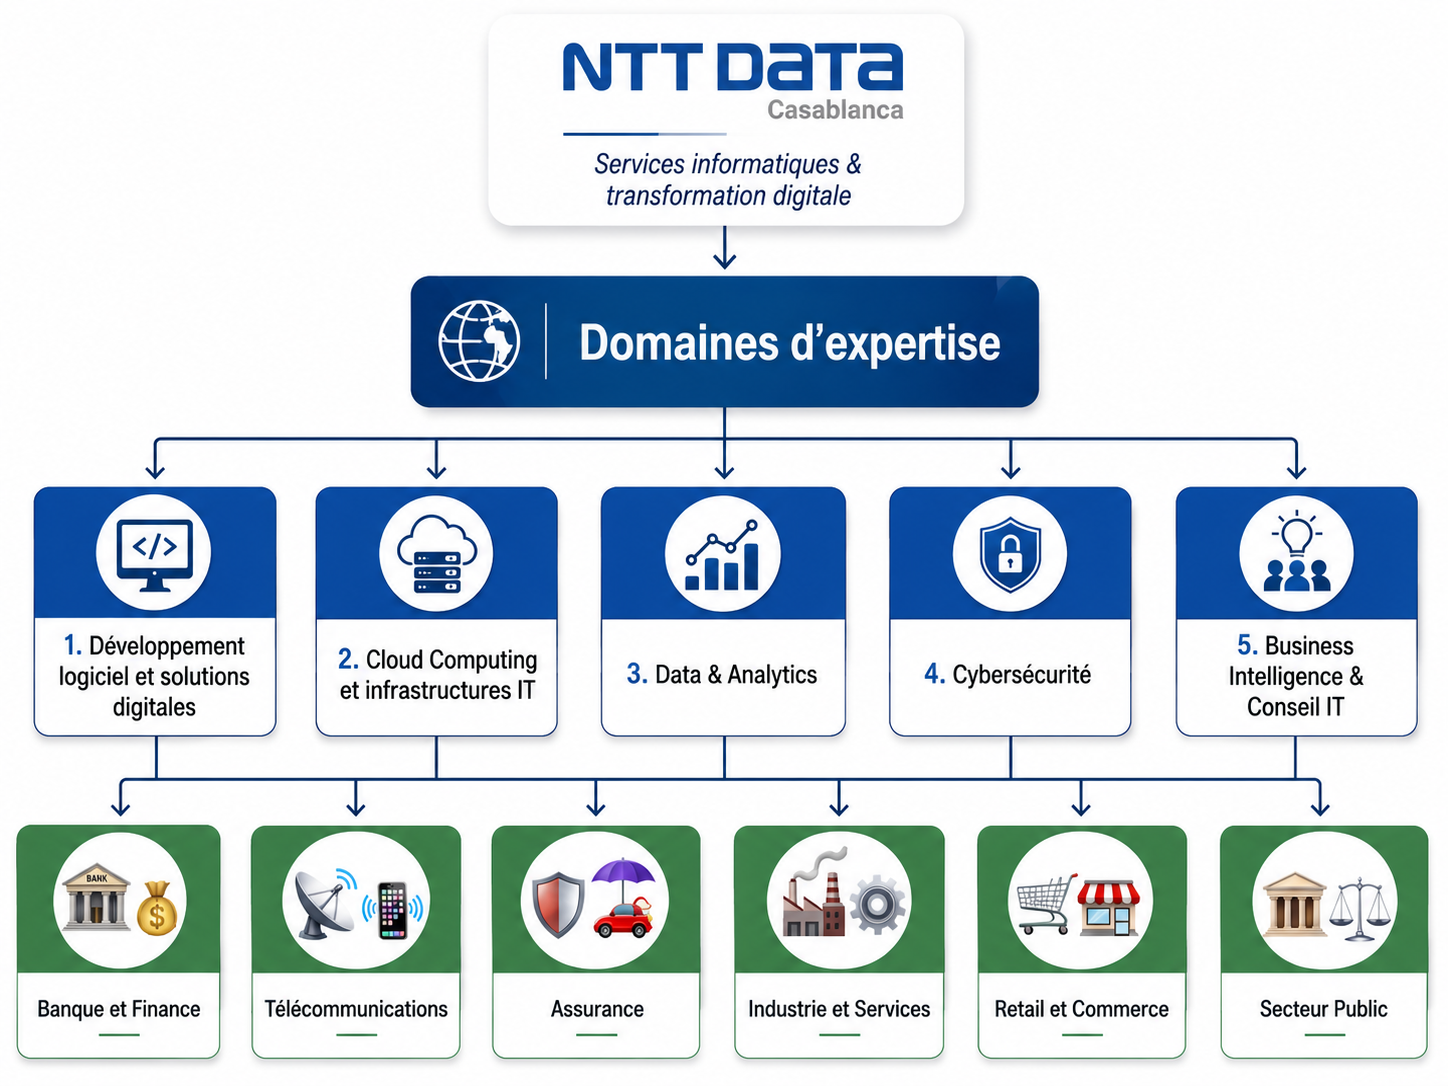
\includegraphics[width=0.8\linewidth]{assets/org.png}
	\caption{Domaines d’expertise et secteurs d’intervention de NTT DATA Casablanca}
	\label{fig:domaines_ntt}
\end{figure}

Comme l’illustre la figure \ref{fig:domaines_ntt}, NTT DATA Maroc structure ses domaines d’expertise autour de cinq pôles principaux :

\begin{enumerate}
    \item \textbf{Développement logiciel et solutions digitales} : conception et réalisation d’applications sur mesure, intégration de systèmes, accompagnement dans la transformation numérique.
    \item \textbf{Cloud Computing et infrastructures IT} : déploiement et gestion d’infrastructures cloud hybrides, migration d’applications, optimisation des ressources.
    \item \textbf{Data \& Analytics} : collecte, traitement et analyse de données massives, mise en place de data lakes, exploitation décisionnelle.
    \item \textbf{Cybersecurity} : audits de sécurité, protection des systèmes d’information, conformité aux normes et régulations.
    \item \textbf{Business Intelligence \& Conseil IT} : tableaux de bord décisionnels, indicateurs de performance, accompagnement stratégique des projets.
\end{enumerate}

L’entreprise intervient principalement dans les secteurs suivants : banque et finance, télécommunications, assurance, industrie et services, retail et commerce, ainsi que le secteur public.

\subsubsection{Présence internationale}
La figure \ref{fig:map_ntt} illustre la présence géographique de NTT DATA à travers le monde.

\begin{figure}[H]
	\centering
	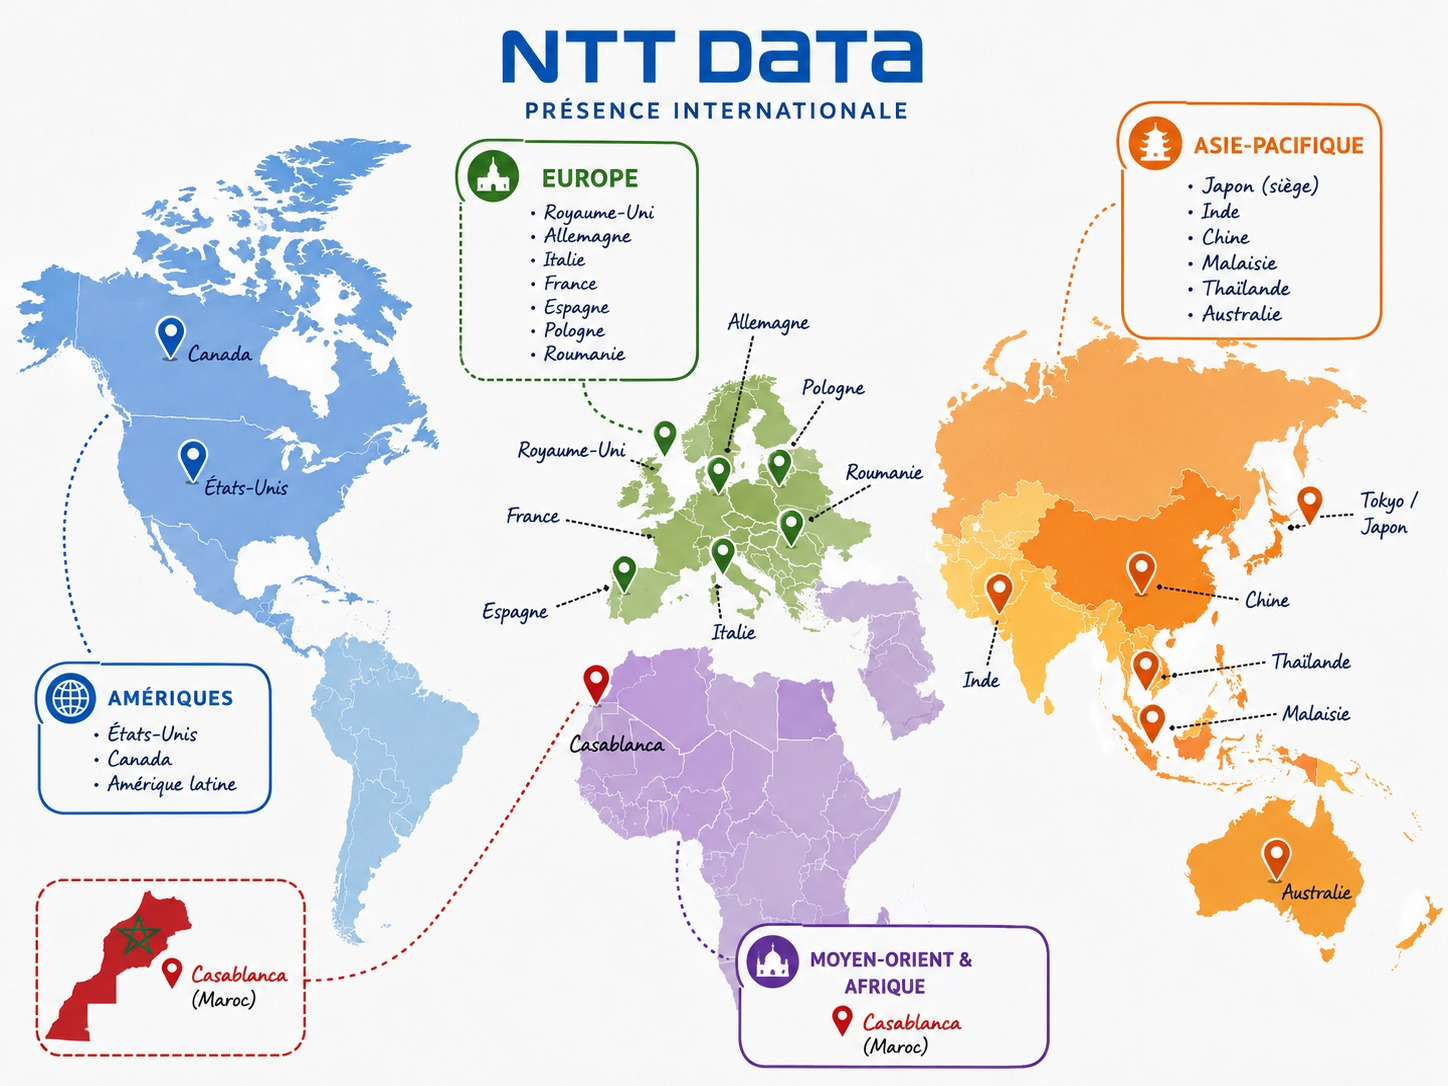
\includegraphics[width=0.8\linewidth]{assets/presence_international.jpeg}
	\caption{Présence géographique de NTT DATA dans le monde}
	\label{fig:map_ntt}
\end{figure}

NTT DATA dispose d’une présence stratégique sur plusieurs continents, avec des bureaux clés notamment :
\begin{itemize}
	\renewcommand{\labelitemi}{—}
	\item \textbf{Tokyo (siège mondial)} : Plus de 150 000 collaborateurs dans le monde
	\item \textbf{Casablanca, Tétouan} : Sièges social pour l’Afrique, moteur de la transformation digitale au Maroc
	\item \textbf{Paris} : Centre européen majeur
	\item \textbf{Washington} : Hub stratégique pour l’Amérique du Nord
	\item \textbf{Dubaï} : Base pour les opérations au Moyen‑Orient
\end{itemize}

\subsection{Structure organisationnelle de l’entreprise}

La Figure \ref{fig:secteurs-nttdata} illustre la structure organisationnelle de la filiale marocaine de NTT DATA. Bien que l'entreprise fasse partie d'un groupe mondial, elle dispose d'une organisation locale agile pour répondre aux enjeux du marché marocain et à ses objectifs de création de plusieurs emplois d'ici 2026.

\begin{figure}[H]
    \centering
    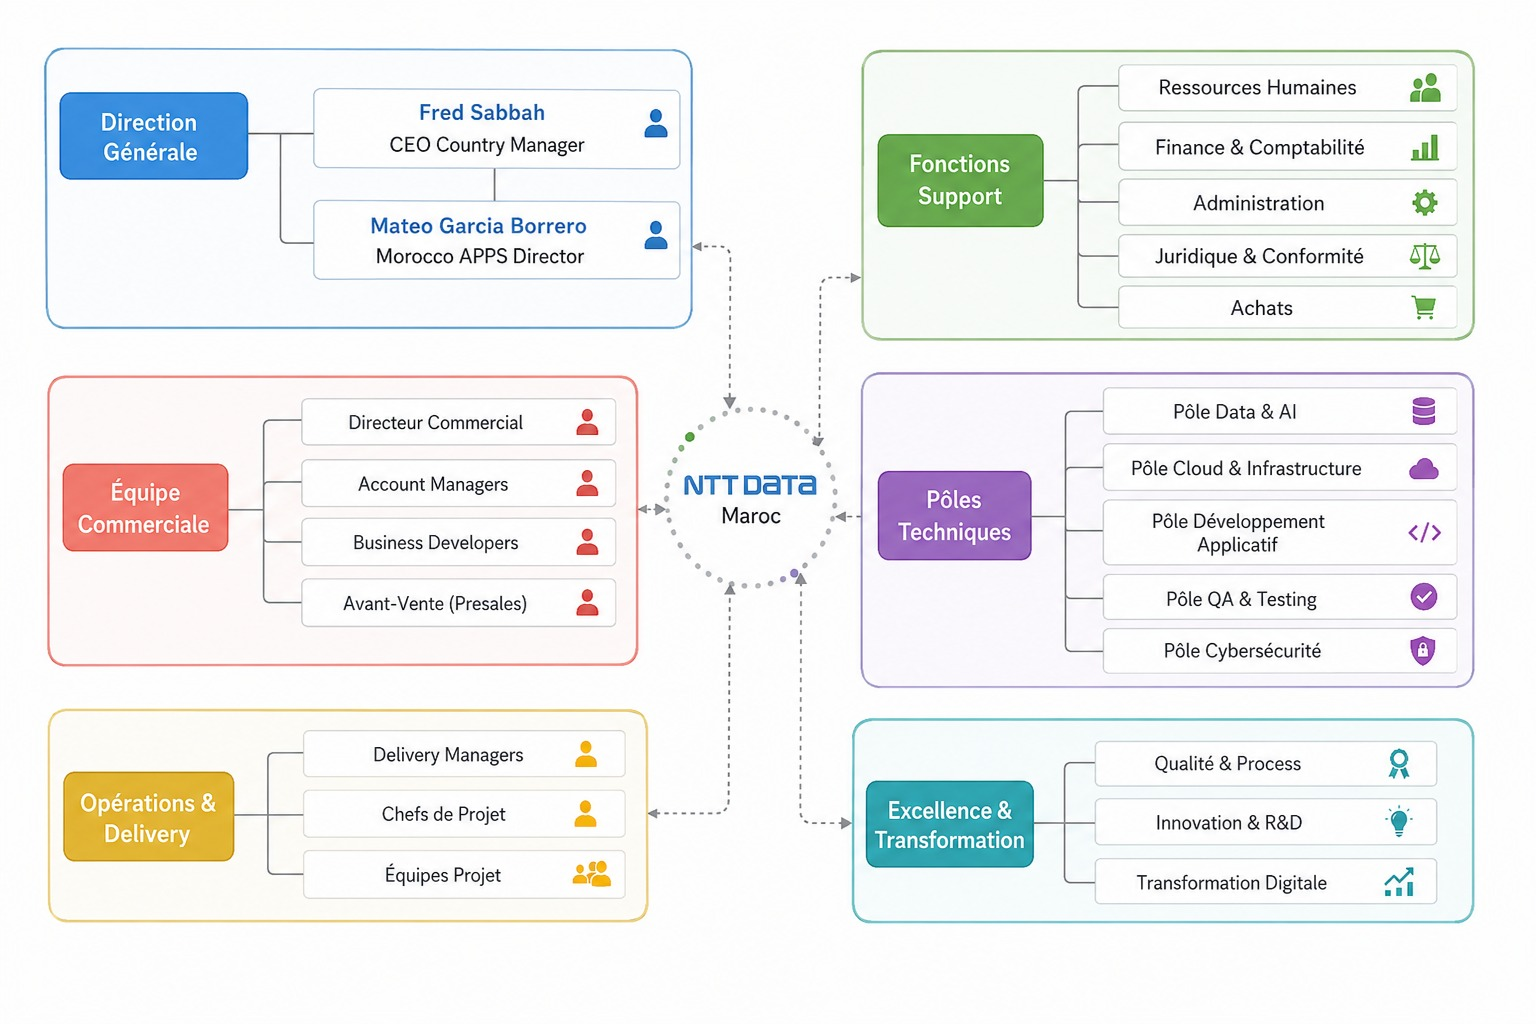
\includegraphics[width=1\linewidth]{assets/logos/secteurs_de_travail.jpeg}
    \caption{Organigramme fonctionnel des principaux pôles de NTT DATA Maroc}
    \label{fig:secteurs-nttdata}
\end{figure}

L'organigramme de NTT DATA Maroc s'articule autour des entités et pôles suivants :

\begin{enumerate}
    \item \textbf{Direction Générale}: Basée à Casablanca, elle est dirigée par le Country Manager, Frédéric Sabbah. Cette équipe définit la vision stratégique et pilote la croissance de l'entreprise au Maroc, en étroite collaboration avec la direction pour la région Moyen-Orient et Afrique.

    \item \textbf{Pôles Techniques et d'Expertise}: Ils constituent le cœur opérationnel de l'entreprise et sont structurés pour délivrer des solutions complètes à ses clients. On y retrouve notamment:
        \begin{itemize}
		\renewcommand{\labelitemi}{—}
            \item Un pôle \textbf{Cloud, Infrastructure et Sécurité}.
            \item Un pôle \textbf{Data \& Intelligence Artificielle (IA)}.
            \item Un pôle dédié aux \textbf{Applications d'entreprise}, avec une expertise particulière sur les solutions SAP.
            \item Un pôle \textbf{Business Process Services (BPS)} pour l'externalisation de processus métier.
        \end{itemize}

    \item \textbf{Équipe Commerciale (Sales) et Marketing}: Chargée du développement du portefeuille clients, de la prospection commerciale et de la gestion des offres de services sur le marché marocain.

    \item \textbf{Équipe des Opérations et du Recrutement}: Essentielle à la stratégie de croissance de l'entreprise, cette équipe gère la livraison des services (notamment pour le pôle BPS) et assure l'acquisition des talents pour atteindre l'objectif ambitieux de création d'emplois.

    \item \textbf{Équipe Administrative et des Ressources Humaines (RH)}: Sous la supervision de la direction, cette équipe gère l'ensemble des aspects financiers, comptables, juridiques et administratifs, ainsi que la gestion du personnel.
\end{enumerate}


\subsection{Contexte interne : utilisation de Jira Data Center}
La gestion de projets logiciels chez NTT DATA génère des volumes croissants de données opérationnelles, principalement via l’outil Jira. Chaque projet peut comporter des centaines, voire des milliers de tickets (tâches, bugs, évolutions), dont l’analyse manuelle pour la détection des risques, des goulots d’étranglement et des retards est devenue trop lente, peu fiable et inadaptée aux exigences de réactivité des équipes. Les chefs de projet et les équipes techniques consacrent un temps considérable à la supervision détaillée de chaque ticket, sans pouvoir bénéficier d’une vision synthétique et prédictive en temps réel.

Face à ce constat, une initiative de modernisation du pilotage de projet a été lancée. L’objectif est de concevoir une plateforme complète, articulée autour d’un \textbf{agent IA conversationnel} comme cœur intelligent, capable d’interagir avec les données Jira de manière autonome et continue. Cette plateforme intègre plusieurs composantes clés :

\begin{itemize}
	\renewcommand{\labelitemi}{—}
    \item Un moteur d’analyse IA qui extrait, normalise et interprète les données Jira pour détecter automatiquement les risques (retards, dépendances critiques, sous-charge ou surcharge d’affectation) et proposer des actions correctives.
    \item Un tableau de bord de monitoring qui offre une vue d’ensemble synthétique, permettant aux responsables de suivre l’état de santé des projets sans avoir à examiner chaque ticket manuellement.
    \item Des simulations Monte Carlo pour prédire la date de fin probable des projets, en prenant en compte l’incertitude des durées et des aléas de développement.
    \item Un explorateur Jira qui structure et visualise les données issues de Jira sous une forme claire et ergonomique.
    \item Un système de contrôle d’accès (RBAC) garantissant que chaque utilisateur (chef de projet, développeur, manager) ne voit que les informations correspondant à son périmètre.
	\item Un système d’alertes automatiques couplé à Microsoft Teams, permettant de notifier instantanément le top management en cas de détection de risque critique.
	\item Une industrialisation complète via un pipeline Jenkins, assurant l’intégration continue, les tests et le déploiement automatisé de la plateforme sur les serveurs de NTT DATA.
	\item Une architecture multi-agents spécialisée, incluant des agents dédiés à l’analyse fine des performances individuelles et collectives (Team Scoreboard et Worker Insights), afin d’optimiser la répartition de la charge de travail.
	\item Une stack d’observabilité technique (Prometheus et Grafana) garantissant la supervision en temps réel de la santé de l’application, des performances du système et des métriques liées à l’intelligence artificielle.
	\item Des métriques avancées et indicateurs de performance (KPIs) permettant d’évaluer en profondeur la dynamique de l’équipe et l’efficacité globale des développements.
\end{itemize}

Cette plateforme répond à un besoin urgent d’accélération de l’analyse : là où une équipe humaine mettrait plusieurs heures ou jours à détecter un risque émergent, l’agent IA opère 24h/24 et 7j/7, fournissant des alertes quasi immédiates. Elle permet également de surmonter les goulots d’étranglement liés à la supervision manuelle détaillée, en libérant du temps pour les tâches à forte valeur ajoutée. Enfin, la capacité prédictive (Monte Carlo) offre une aide à la décision proactive, transformant la gestion de projet réactive en une gestion anticipative et stratégique.

Ainsi, le projet consiste à développer et intégrer l’ensemble de ces briques pour fournir à NTT DATA un outil innovant, permanent et fiable de pilotage de projet par l’IA.

\section{Présentation du projet}
Nous allons à présent détailler le projet sur lequel nous avons travaillé, en commençant par
son contexte, ses enjeux et les objectifs visés.
\subsection{Contexte du projet}

La gestion de projets logiciels chez NTT DATA est en pleine mutation, confrontée à des besoins croissants en matière de réactivité, de fiabilité et d’anticipation des risques. Chaque projet génère des centaines, voire des milliers de tickets Jira (tâches, bugs, évolutions), dont l’analyse manuelle devient trop lente, fastidieuse et inadaptée aux exigences opérationnelles. Dans ce contexte, une initiative de modernisation du pilotage de projet a été lancée pour optimiser la détection des risques et des goulots d’étranglement, en particulier pour les équipes de NTT DATA Maroc.

Cette plateforme innovante se fonde sur le développement d’un \textbf{agent IA conversationnel} capable d’extraire, de normaliser et d’analyser en continu les données issues de Jira. L’objectif global est de fournir aux chefs de projet et aux équipes techniques une vision synthétique et prédictive, avec des alertes automatiques sur les retards, les dépendances critiques et les anomalies d’affectation, ainsi que des recommandations d’actions correctives.

Cette modernisation vise également à répondre à des besoins urgents d’accélération de l’analyse : là où une équipe humaine mettrait plusieurs heures ou jours à détecter un risque émergent, l’agent IA opère 24h/24 et 7j/7, délivrant des informations quasi immédiates. Elle permet de dépasser les limites de la supervision manuelle détaillée, trop lourde à l’échelle de nombreux tickets, et de libérer du temps pour les tâches à forte valeur ajoutée. En raison d’un souci d’implémentation progressive, le projet a été décliné en différentes briques fonctionnelles : tableau de bord de monitoring, simulation Monte Carlo pour la prédiction des dates de fin de projet, explorateur Jira structuré, et système de contrôle d’accès par rôles (RBAC). La première étape concerne notamment l’intégration de l’agent IA conversationnel comme cœur intelligent de la plateforme, pour une détection proactive des risques et des actions recommandées.

\subsection{Problématique du projet}

La gestion des projets logiciels chez NTT DATA, à travers l’outil Jira, constitue un défi opérationnel majeur, notamment lorsque les volumes de données deviennent massifs et que les équipes doivent superviser des centaines de tickets simultanément.

Actuellement, les pratiques d’analyse et de pilotage se heurtent à :
\begin{itemize}
    \renewcommand{\labelitemi}{—}
    \item un volume de données massif (tickets, commentaires, historiques) rendant l’exploitation manuelle fastidieuse.
    \item une hétérogénéité des champs Jira selon les projets, empêchant toute normalisation automatique des informations.
    \item une absence totale de détection automatique des anomalies (tickets bloqués, délais dépassés, dépendances critiques).
    \item une réactivité limitée des équipes de pilotage, contraintes à une supervision séquentielle et chronophage.
    \item une absence de notification instantanée des risques vers le top management, les décisions correctives étant souvent prises avec un retard préjudiciable.
    \item un déploiement manuel des outils de pilotage, sans intégration ni livraison continues, ce qui freine l’industrialisation des solutions.
\end{itemize}

Cela conduit à des risques non identifiés à temps, des retards qui se propagent en cascade, une sous-utilisation des capacités prédictives, une réactivité managériale limitée et une difficulté à maintenir les outils en condition opérationnelle. L’absence d’un mécanisme d’intelligence artificielle capable d’extraire, normaliser et analyser en continu les données Jira, couplé à un pipeline de déploiement automatisé, limite fortement la capacité des équipes à anticiper les problèmes et à proposer des actions correctives rapidement.

La problématique est donc de concevoir une plateforme intelligente, articulée autour d’un agent IA conversationnel, capable d’analyser en temps réel les données Jira, de détecter automatiquement les risques et les goulots d’étranglement, de générer des recommandations actionnables, de notifier instantanément le management (Microsoft Teams) et de s’intégrer dans une chaîne d’industrialisation (Docker, Jenkins). La solution doit également offrir une vision prédictive (Monte Carlo) et un tableau de bord de monitoring adapté aux besoins des chefs de projet et des équipes techniques.


\subsection{Objectifs généraux du projet}

Ce projet vise à moderniser le pilotage des projets logiciels chez NTT DATA à travers la mise en place d’une plateforme full‑stack intelligente, articulée autour d’un agent IA conversationnel, d’un tableau de bord de monitoring, de simulations prédictives, d’une stack d’observabilité et d’un système de contrôle d’accès sécurisé. L’objectif principal est de renforcer la performance et la réactivité des équipes de gestion de projet en leur fournissant des outils d’analyse automatique des risques, de détection des goulots d’étranglement, de prédiction et d’aide à la décision.

La démarche s’articule autour de plusieurs axes stratégiques :

\begin{itemize}
    \renewcommand{\labelitemi}{—}
    \item Développer un agent IA (LangGraph + Mistral) pour l’extraction, la normalisation et l’analyse en continu des données Jira, avec génération automatique de risques et de recommandations.
    \item Concevoir un tableau de bord de métriques et de visualisations (React) offrant aux chefs de projet une vue synthétique et en temps réel de la santé des projets.
    \item Mettre en place une authentification sécurisée par rôles (RBAC, JWT, PostgreSQL) pour garantir la confidentialité et la granularité des accès selon les profils utilisateurs.
    \item Intégrer un cache Redis pour optimiser les performances d’accès aux données fréquemment sollicitées.
    \item Industrialiser la solution via Docker (conteneurisation) et Jenkins (intégration et déploiement continus).
    \item Déployer une stack de supervision (Prometheus, Grafana, Alertmanager) pour collecter les métriques système et applicatives, visualiser la santé des projets en temps réel et déclencher des alertes.
    \item Mettre en place un système de notification automatique vers Microsoft Teams afin d’alerter instantanément le top management en cas de risque critique.
    \item Développer un tableau de bord des performances individuelles (Team Scoreboard) permettant d’analyser la charge, la vélocité et la productivité de chaque membre de l’équipe.
\end{itemize}

\subsection{Objectifs spécifiques de la plateforme IA}

Dans cette première phase, l’objectif est de développer une solution dédiée à l’analyse automatique des risques projet à partir des tickets Jira.

La solution devra :

\begin{itemize}
    \renewcommand{\labelitemi}{—}
    \item Extraire et normaliser les tickets Jira via l’API REST, en gérant l’hétérogénéité des champs entre les projets.
    \item Calculer des signaux de santé projet (WIP ratio, stale ratio, overdue rate, coefficient de Gini) à partir des données historiques et en temps réel.
    \item Implémenter un moteur de règles combiné à un LLM (Mistral hébergé à Tétouan, accessible via API) pour générer des risques, des actions correctives et des recommandations contextuelles.
    \item Fournir une interface React avec visualisations de métriques, un explorateur Jira structuré et un tableau de bord des performances individuelles.
    \item Assurer la sécurité des échanges (JWT) et la gestion fine des rôles utilisateurs.
    \item Conteneuriser l’application avec Docker et orchestrer le déploiement via Jenkins.
    \item Implémenter des simulations de Monte Carlo pour prédire la date de fin des projets en fonction de la vélocité historique et du backlog restant (percentiles p50 à p95).
    \item Superviser l’état de santé de l’application via Prometheus et Grafana, avec des règles d’alerte personnalisées (ex. \texttt{CriticalWipRatio}, \texttt{ProjectAtRisk}).
\end{itemize}

L’approche proposée repose sur l’utilisation d’algorithmes d’intelligence artificielle et d’un agent conversationnel capable d’opérer 24h/24 et 7j/7, couplé à une stack d’observabilité moderne, permettant non seulement de réduire les délais de détection des anomalies, mais aussi d’anticiper les retards, d’alerter proactivement le management et de maximiser la réactivité des équipes de pilotage.
Ce travail constitue une première brique essentielle, posant les bases techniques et méthodologiques sur lesquelles s’appuieront les prochaines phases du projet, visant à étendre l’analyse prédictive (simulations Monte Carlo) et l’optimisation à d’autres dimensions de la gestion de projet (budget, ressources humaines, qualité logicielle).

\subsection{Conduite du projet}

Cette section présente la méthodologie et la planification du projet, en décrivant les approches et étapes clés pour sa réussite.

\subsubsection{Méthodologie de travail}

La méthodologie adoptée est Scrum, une approche agile itérative qui facilite le suivi du projet, encourage l’adaptabilité, la collaboration et l’amélioration continue à travers des sprints courts.

\begin{figure}[H]
	\centering
	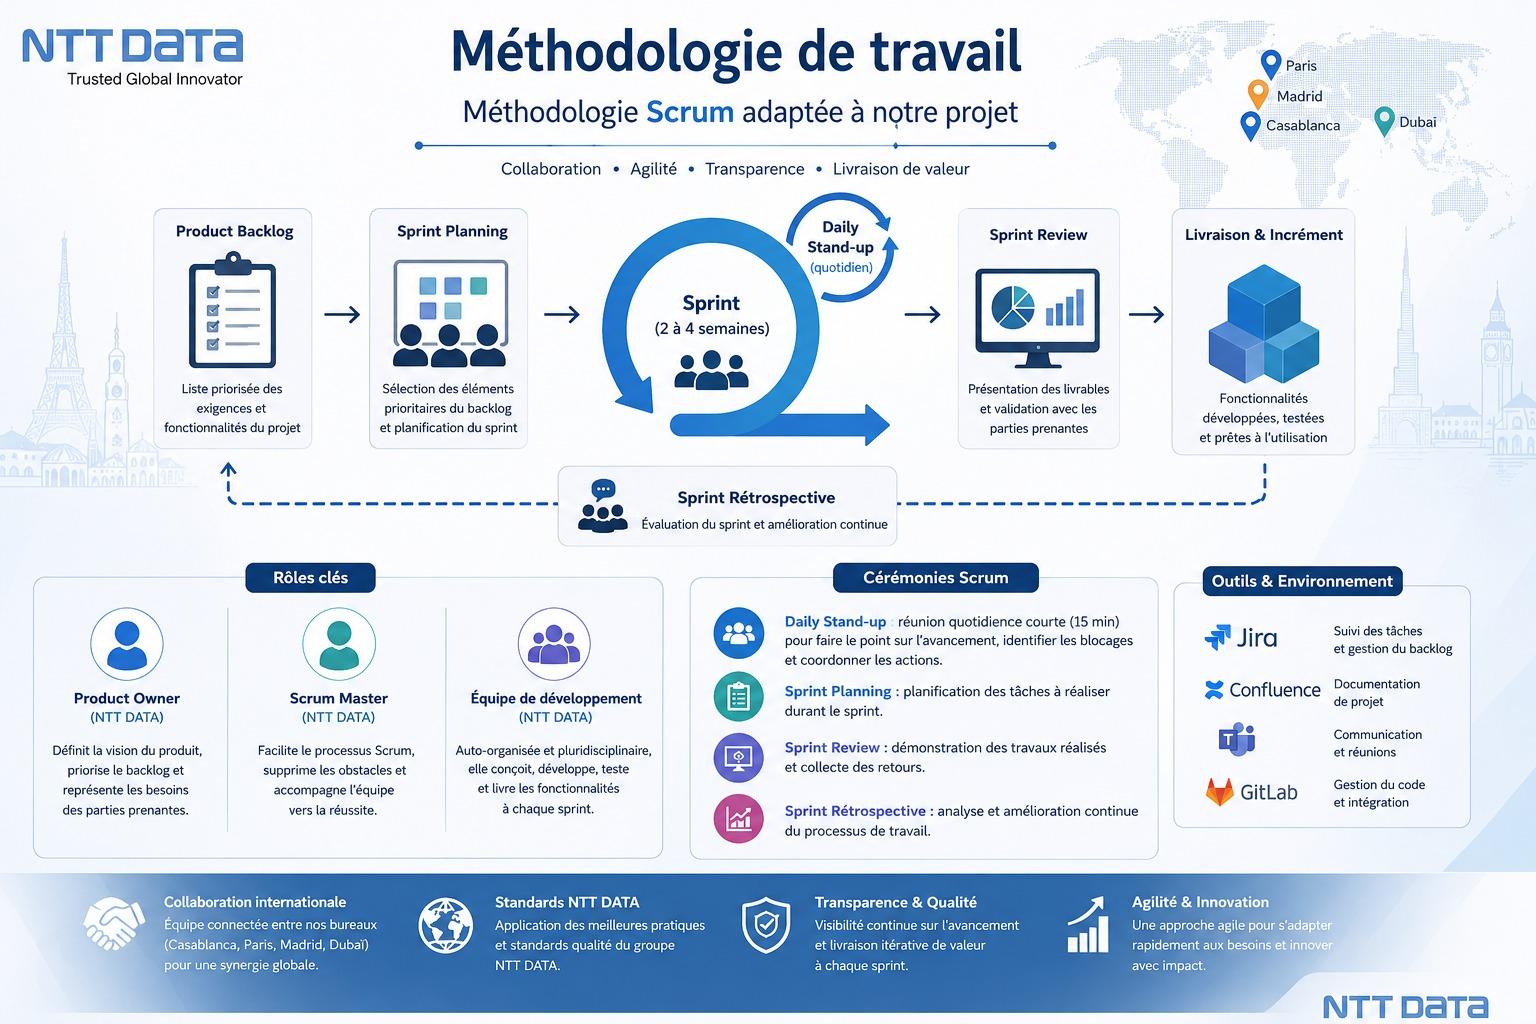
\includegraphics[width=0.8\linewidth]{assets/methodologie_travail.jpeg}
	\caption{Méthodologie agile Scrum adoptée pour le projet}
	\label{fig:scrum_ntt}
\end{figure}

\paragraph{Les rôles Scrum dans notre projet}

Les trois rôles principaux dans notre projet sont les suivants :

\begin{itemize}
	\renewcommand{\labelitemi}{—}
	\item \textbf{Product Owner} : Le top management de NTT DATA Maroc (direction générale), responsable de la vision stratégique, du backlog prioritaire et de la validation des livrables.
	\item \textbf{Scrum Master} :  Mohammed Amine Elmeknassi, supervise le processus Scrum, organise les réunions quotidiennes, répartisse les tâches et identifient les blocages.
	\item \textbf{Équipe Intelligence Artificielle} : composée de moi-même, Nour Derraz et Image Chaoui, responsable de la conception de l’agent IA, du développement de la plateforme full‑stack, de l’analyse des données Jira et de la documentation technique.
\end{itemize}

\paragraph{Cérémonies Scrum}

Chaque jour, de 9h à 9h45, nous tenons un \textbf{Daily Stand-up} à distance (visioconférence) avec Mohammed Amine Elmeknassi. Cette réunion sert à faire le point sur l’avancement, identifier les blocages et coordonner les actions. La majorité du travail s’effectue à distance, avec une présence physique au bureau de NTT DATA Casablanca une fois par semaine pour les réunions de synthèse.

Chaque semaine, nous produisons une présentation (PPT) listant l’ensemble des réalisations accomplies. Mohammed Amine Elmeknassi transmet ce compte rendu à Anis Khairi, puis ils le remontent au top management de NTT DATA Maroc afin de suivre l’avancement global du projet.

Avant chaque sprint, la \textbf{Sprint Planning Meeting} permet de sélectionner les éléments prioritaires du Product Backlog à développer. La \textbf{Sprint Review} présente les fonctionnalités développées aux parties prenantes, notamment le top management de NTT DATA Maroc et les responsables techniques.

\subsubsection{Planification du projet}

Bien que Scrum repose sur une gestion itérative des priorités, un diagramme de Gantt a été utilisé pour visualiser les grandes étapes du projet (développement de l’agent IA, intégration de l’API Jira, mise en place du tableau de bord, simulation Monte Carlo, RBAC, déploiement Docker/Jenkins), leur enchaînement et leurs dépendances.
\begin{figure}[H]
	\centering
	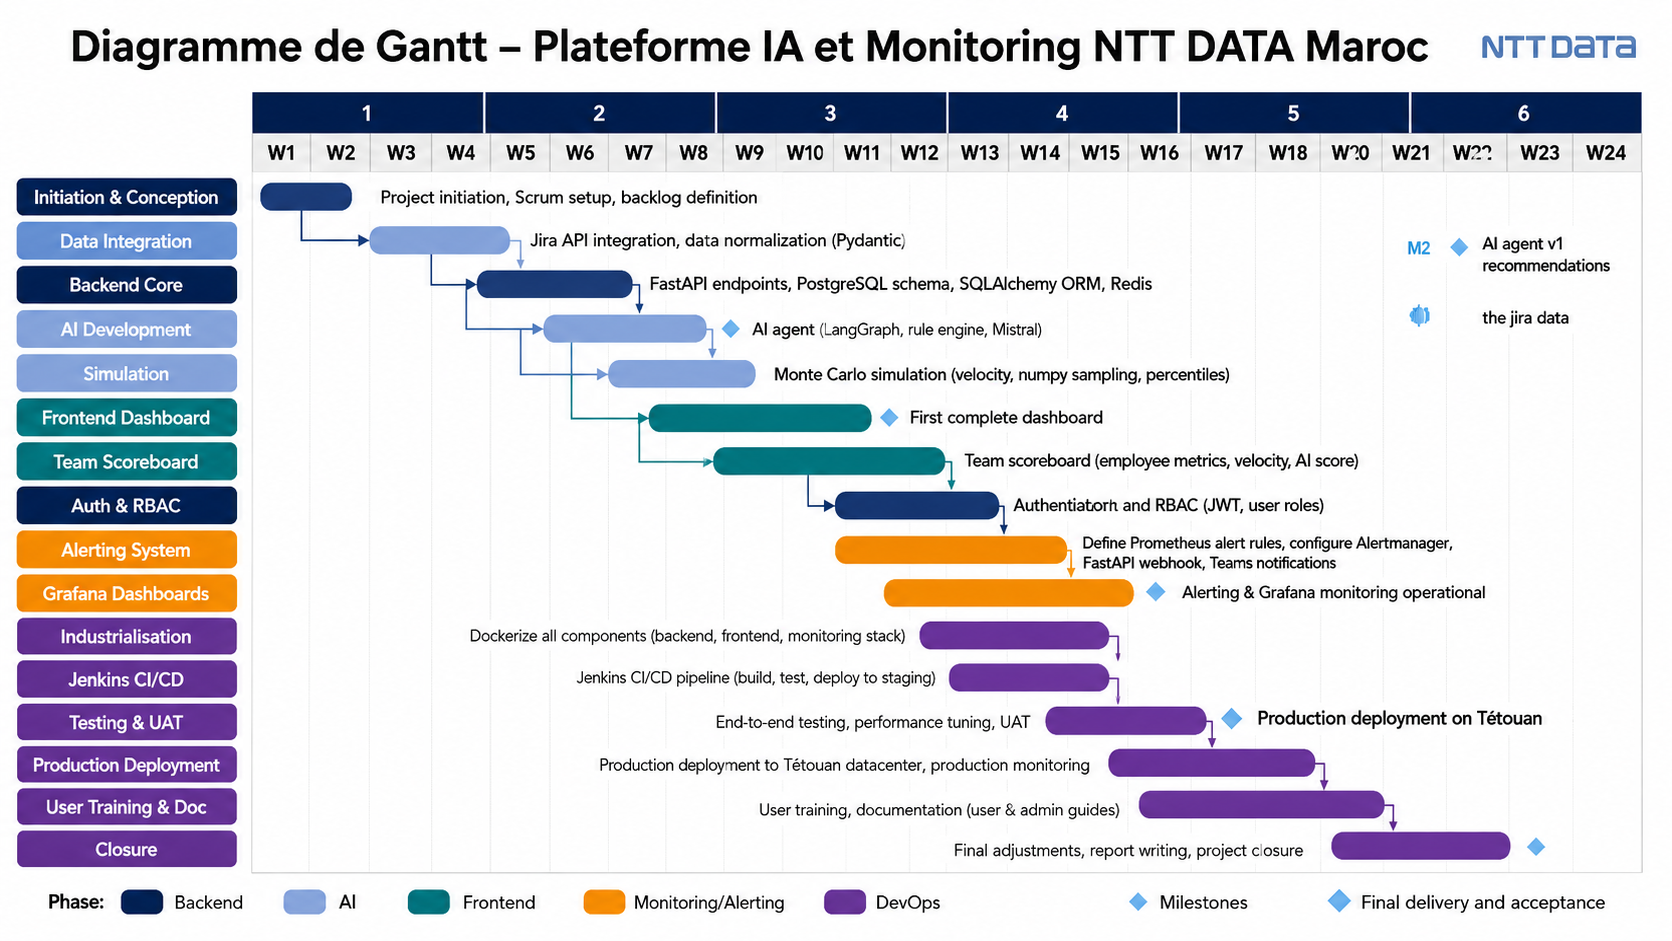
\includegraphics[width=0.8\linewidth]{assets/diagram_gant.png}
	\caption{Diagramme de Gantt illustrant la planification globale du projet}
	\label{fig:gant_ntt}
\end{figure}


\section{Conclusion}

Pour conclure ce premier chapitre, nous avons présenté NTT DATA Maroc en soulignant son contexte historique, son activité et sa structure organisationnelle. Nous avons également exposé la problématique du projet – la lenteur et le manque de fiabilité de l’analyse manuelle des tickets Jira – ainsi que les objectifs généraux et spécifiques de la plateforme à agent IA. Enfin, nous avons abordé la méthodologie Scrum adoptée, les rôles de l’équipe, les cérémonies quotidiennes et hebdomadaires, ainsi que la planification globale. Dans le prochain chapitre, nous aborderons l’analyse des besoins, la conception fonctionnelle ainsi que l’architecture technique du projet.
	\chapter{Conception fonctionnelle et technique}
\vspace{-1.5em}
\chaptertoc
\vspace{-2.5em}
\section{Introduction}
Ce chapitre est dédié à la conception fonctionnelle et technique de la plateforme d'analyse des risques de projet. Il détaille dans un premier temps la phase d'analyse des besoins, fruit d'une démarche itérative menée auprès des parties prenantes, avant de définir de manière exhaustive les exigences fonctionnelles et non fonctionnelles. Cette étape fondamentale permet de poser les jalons de l'architecture logicielle qui sera mise en œuvre pour répondre aux problématiques de suivi soulevées par les équipes de NTT DATA Maroc.

\section{Analyse des besoins}

\subsection{Processus d'identification des besoins}
Le processus de recueil des exigences s'est appuyé sur une démarche hautement collaborative et itérative, essentielle pour s'aligner sur les réalités du terrain. Plusieurs réunions de cadrage et des revues d'avancement hebdomadaires ont été menées en étroite collaboration avec le management et l'équipe d'encadrement, notamment Monsieur Mohammed Amine Elmeknassi et Monsieur Anis Khairi. Ces échanges se sont déroulés selon un format hybride, alliant des ateliers en présentiel dans les locaux de NTT DATA Maroc à Casablanca et des sessions de travail à distance. L'utilisation systématique de présentations lors de ces points d'étape a permis de valider progressivement les hypothèses de conception et de cerner avec précision les attentes des futurs utilisateurs vis-à-vis de l'automatisation par l'intelligence artificielle.

\subsection{Les besoins fonctionnels}
Les fonctionnalités du système ont été définies en fonction des interactions attendues pour chaque acteur clé de la plateforme. En premier lieu, l'agent d'intelligence artificielle agit comme le moteur d'analyse continu du système ; il a pour mission d'interroger l'API Jira de façon autonome, de traiter les descriptions et les commentaires pour y déceler des anomalies, et de générer des recommandations d'actions correctives. En second lieu, l'utilisateur final nécessite un accès interactif à un tableau de bord global. Cet espace doit lui permettre de visualiser les métriques de performance, de consulter les prévisions de la date de fin générées par les simulations de Monte Carlo, et d'exporter ces indicateurs de manière intuitive. En troisième lieu, l'administrateur doit disposer des interfaces nécessaires pour configurer les paramètres globaux de l'application, gérer les comptes utilisateurs et définir finement les niveaux d'autorisation grâce à un système de contrôle d'accès basé sur les rôles. Enfin, l'acteur DevOps requiert des mécanismes automatisés facilitant le déploiement de l'infrastructure conteneurisée, ainsi que des outils permettant de superviser la bonne exécution des tâches d'arrière-plan.

\subsection{Les besoins non fonctionnels}

Afin de garantir une exploitation fiable et fluide en milieu industriel, l'application doit satisfaire des critères non fonctionnels rigoureux. Sur le plan des performances, le système s'engage à fournir des temps d'affichage minimaux de l'interface, rendus possibles par l'implémentation d'un système de mise en cache Redis qui évite le recalcul des métriques lourdes. La sécurité constitue une priorité absolue ; elle est assurée par une authentification stricte basée sur des jetons JWT et par l'utilisation d'un modèle de langage hébergé localement, garantissant ainsi qu'aucune donnée de projet confidentielle ne transite vers des serveurs externes. En matière de disponibilité, la plateforme est conçue pour fonctionner de manière ininterrompue en arrière-plan, s'appuyant sur des processus asynchrones qui assurent un service en continu. La maintenabilité est assurée par une architecture logicielle modulaire séparant clairement l'interface utilisateur des logiques de l'agent IA, facilitant ainsi l'ajout futur de nouveaux indicateurs. L'utilisabilité a été pensée pour offrir une expérience visuelle moderne, favorisant une interprétation instantanée des graphiques complexes. Enfin, l'interopérabilité est garantie par le respect strict des standards d'interface de programmation, permettant au système de s'intégrer de manière transparente avec l'écosystème Jira de l'entreprise.

\section{Analyse de l'existant}

Avant de proposer une solution d’optimisation, il est essentiel d’analyser l’existant afin d’identifier
les forces et les limites du système actuellement en place.

\subsection{Étude de l'existant}
Au sein de NTT DATA Maroc, le pilotage des projets et l'analyse des risques reposent historiquement sur une exploitation classique des outils de gestion de cycle de vie des applications, principalement Jira. Les chefs de projet s'appuient sur les tableaux de bord natifs de la plateforme pour suivre l'avancement global des tâches et identifier visuellement les éventuels points de blocage. Pour répondre aux exigences de reporting du top management, cette approche est couramment complétée par des extractions manuelles de données vers des tableurs Excel, qui sont ensuite souvent intégrées dans des solutions de type Power BI. Ces données agrégées servent finalement de support lors des revues d'avancement hebdomadaires sous forme de présentations. Par ailleurs, bien que des extensions spécialisées du marché telles que BigPicture, EazyBI ou Risk Explorer soient reconnues pour offrir des capacités avancées de visualisation et de gestion de portefeuille, elles demeurent fondamentalement orientées vers l'analyse rétrospective. Actuellement, la détection des risques repose donc presque exclusivement sur l'expertise humaine des chefs de projet, qui doivent examiner individuellement l'état des tickets, vérifier leur ancienneté et interpréter les commentaires pour évaluer la santé réelle d'un projet de développement.

\begin{figure}[!h]
	\centering
	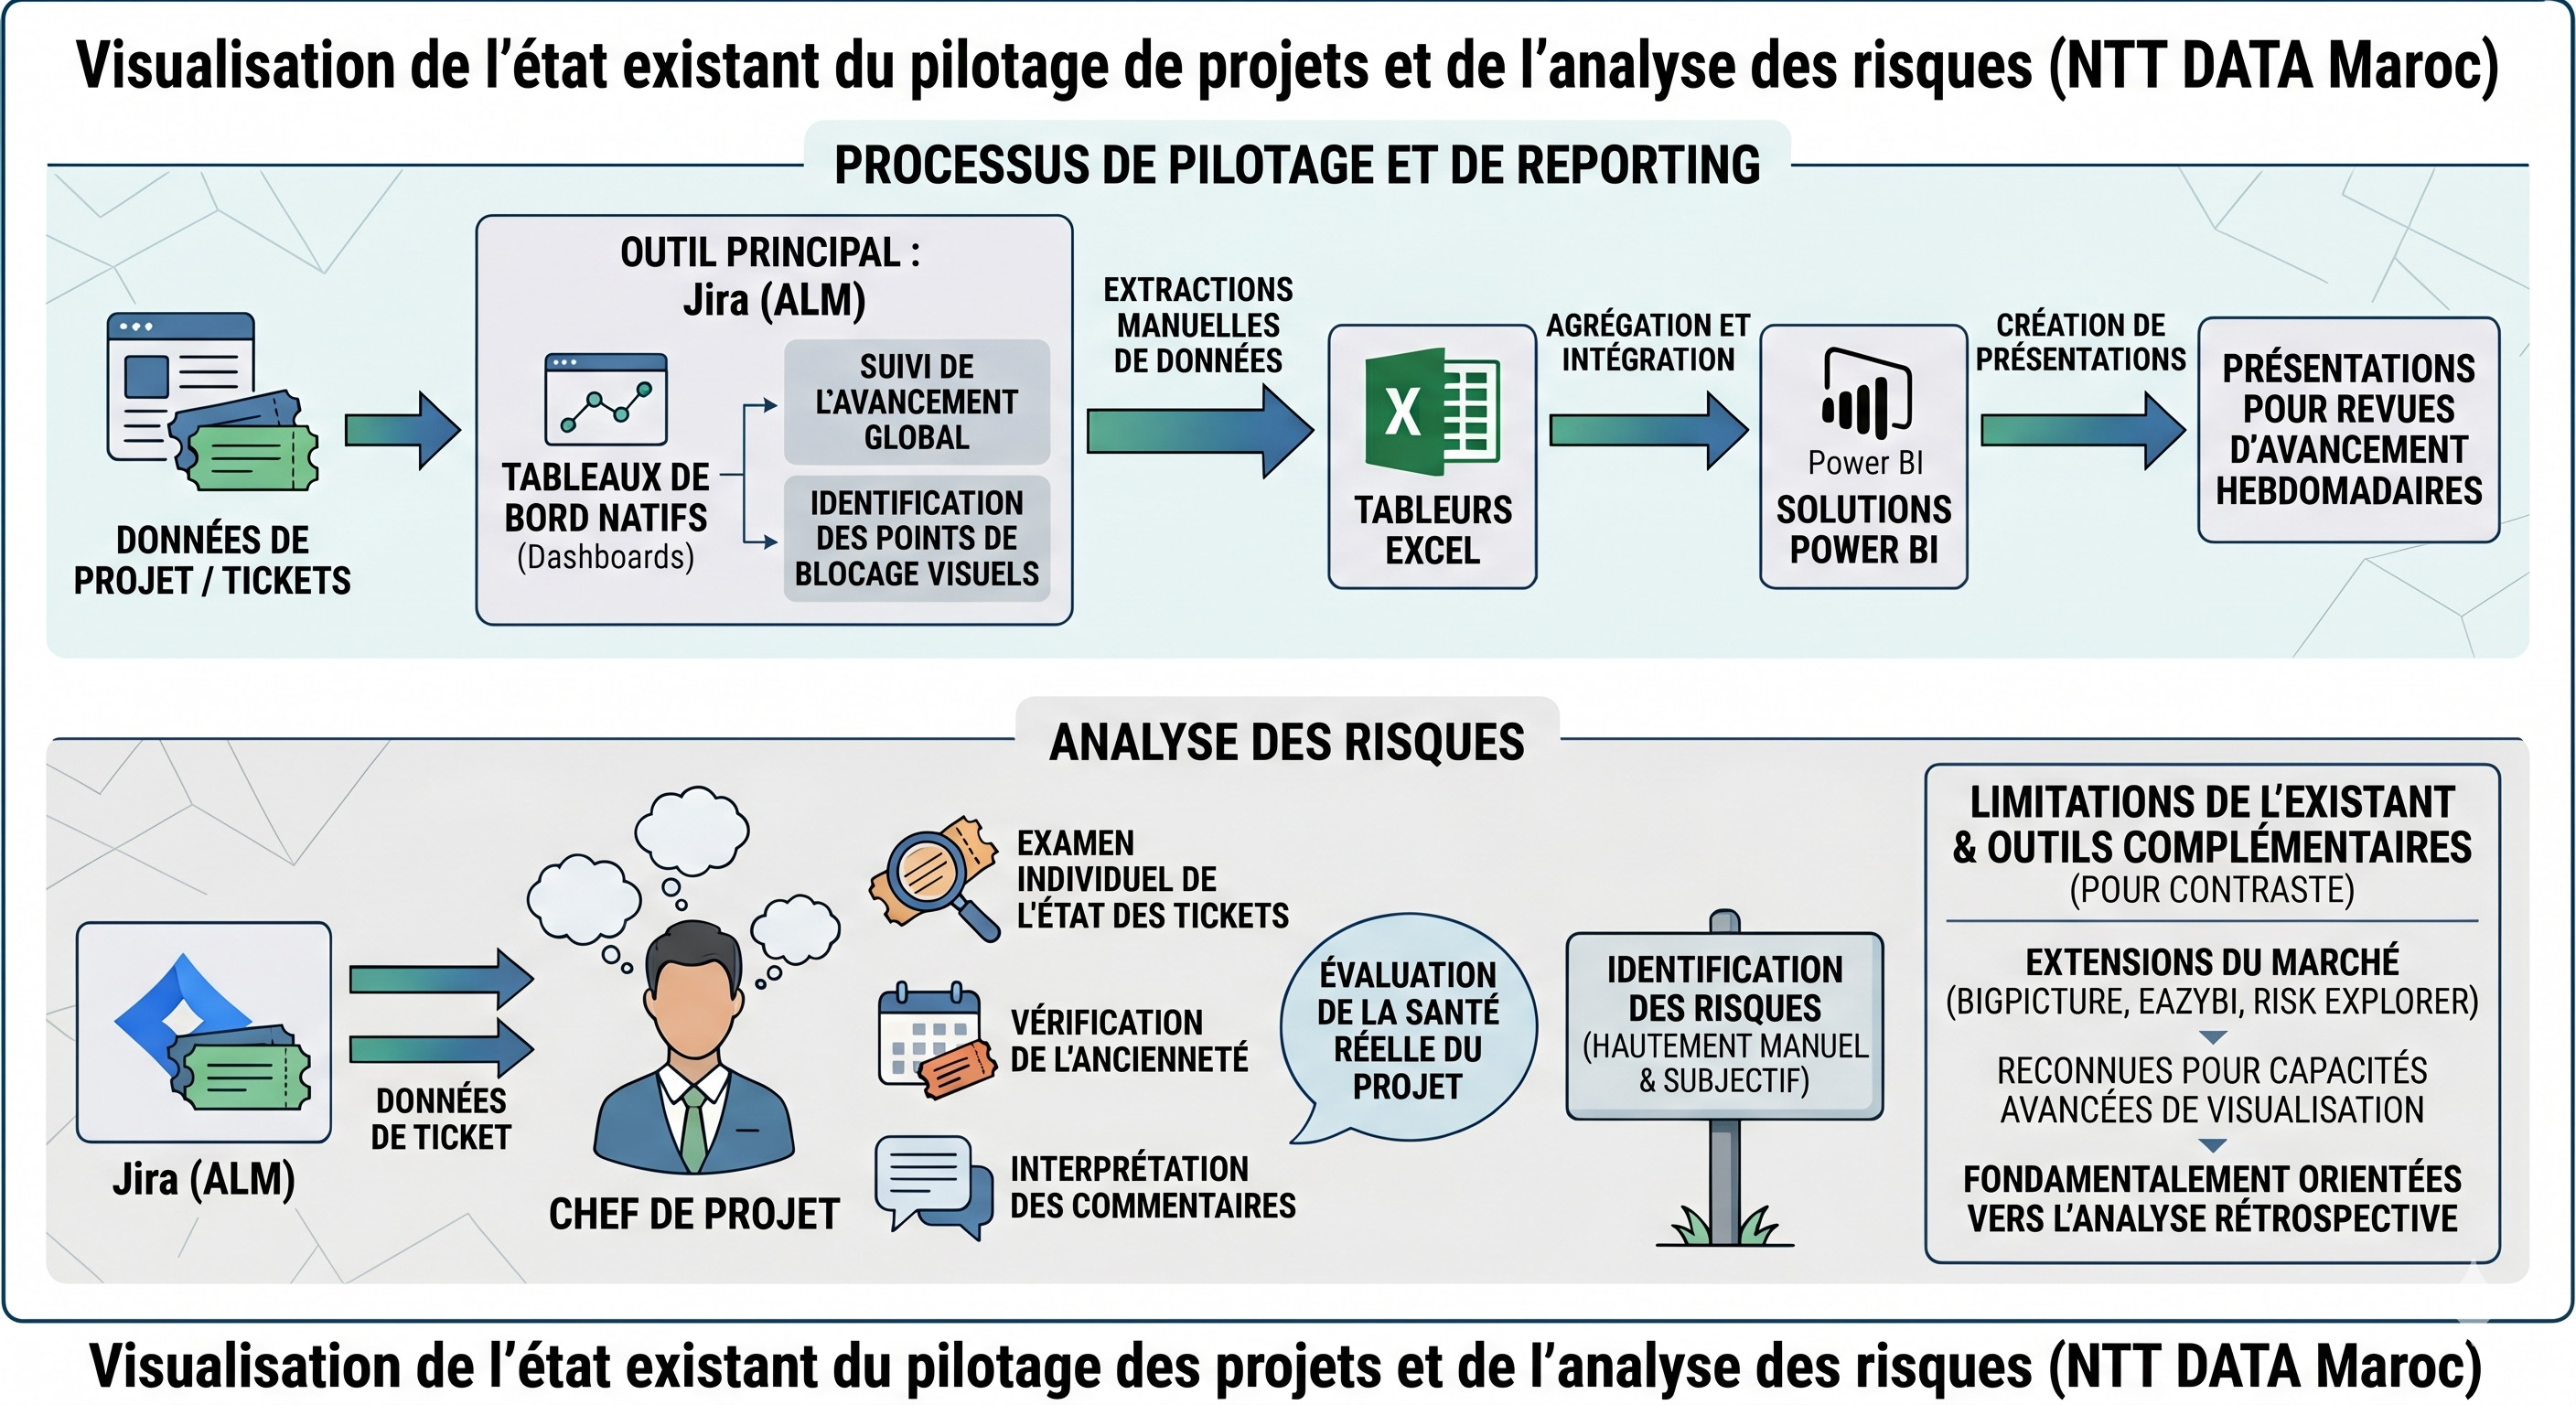
\includegraphics[width=0.9\linewidth]{assets/state_of_existance.png}
	\caption{State of Existance}
	\label{fig:state_existance}
\end{figure}

\subsection{Identification des limitations de l'existant}
Cette approche traditionnelle présente plusieurs limitations majeures qui entravent l'efficacité opérationnelle et la réactivité des équipes :
\begin{enumerate}
    \item \textbf{Caractère hautement chronophage et manuel} : la collecte des indicateurs est une tâche répétitive qui mobilise un temps précieux au détriment de la prise de décision stratégique.
    \item \textbf{Manque d’outils d’analyse prédictive} : l’absence de modèles probabilistes robustes, tels que les simulations de Monte Carlo, oblige les gestionnaires à formuler des estimations de délais basées sur l’intuition plutôt que sur des projections statistiques rigoureuses.
    \item \textbf{Incapacité à exploiter la sémantique des données textuelles} : sans l’apport de l’intelligence artificielle, il est impossible de traiter automatiquement le contenu qualitatif des descriptions et des échanges pour y déceler des signes précoces de dette technique, d’incompréhension des spécifications ou de blocages invisibles.
    \item \textbf{Absence de génération automatique de recommandations} : aucune action correctrice n’est proposée de manière autonome, laissant le chef de projet seul face à l’élaboration de solutions de remédiation.
    \item \textbf{Réaction tardive aux problèmes émergents} : l’absence d’automatisation intelligente fait que les risques ne sont souvent traités qu’après s’être transformés en incidents impactant le calendrier ou le budget.
    \item \textbf{Surcharge cognitive et risque d’omission} : face à l’augmentation constante du volume de tickets dans les projets complexes, l’analyse exclusivement humaine provoque une charge mentale inévitable, augmentant le risque d’oublier des informations critiques.
\end{enumerate}


\subsection{Vue d'ensemble}
Pour répondre aux exigences complexes de l'analyse prédictive et de l'automatisation du suivi de projet, la plateforme s'articule autour d'une architecture distribuée, modulaire et hautement intégrée. Cette conception vise à séparer clairement les responsabilités (extraction de données, calcul intensif, raisonnement par intelligence artificielle et présentation visuelle) afin de garantir à la fois la scalabilité du système, la sécurité absolue des données sensibles et la fluidité de l'interface utilisateur. L'ensemble interagit au travers d'interfaces de programmation (API) standardisées, permettant une évolution indépendante de chaque composant.

\begin{figure}[H]
\centering
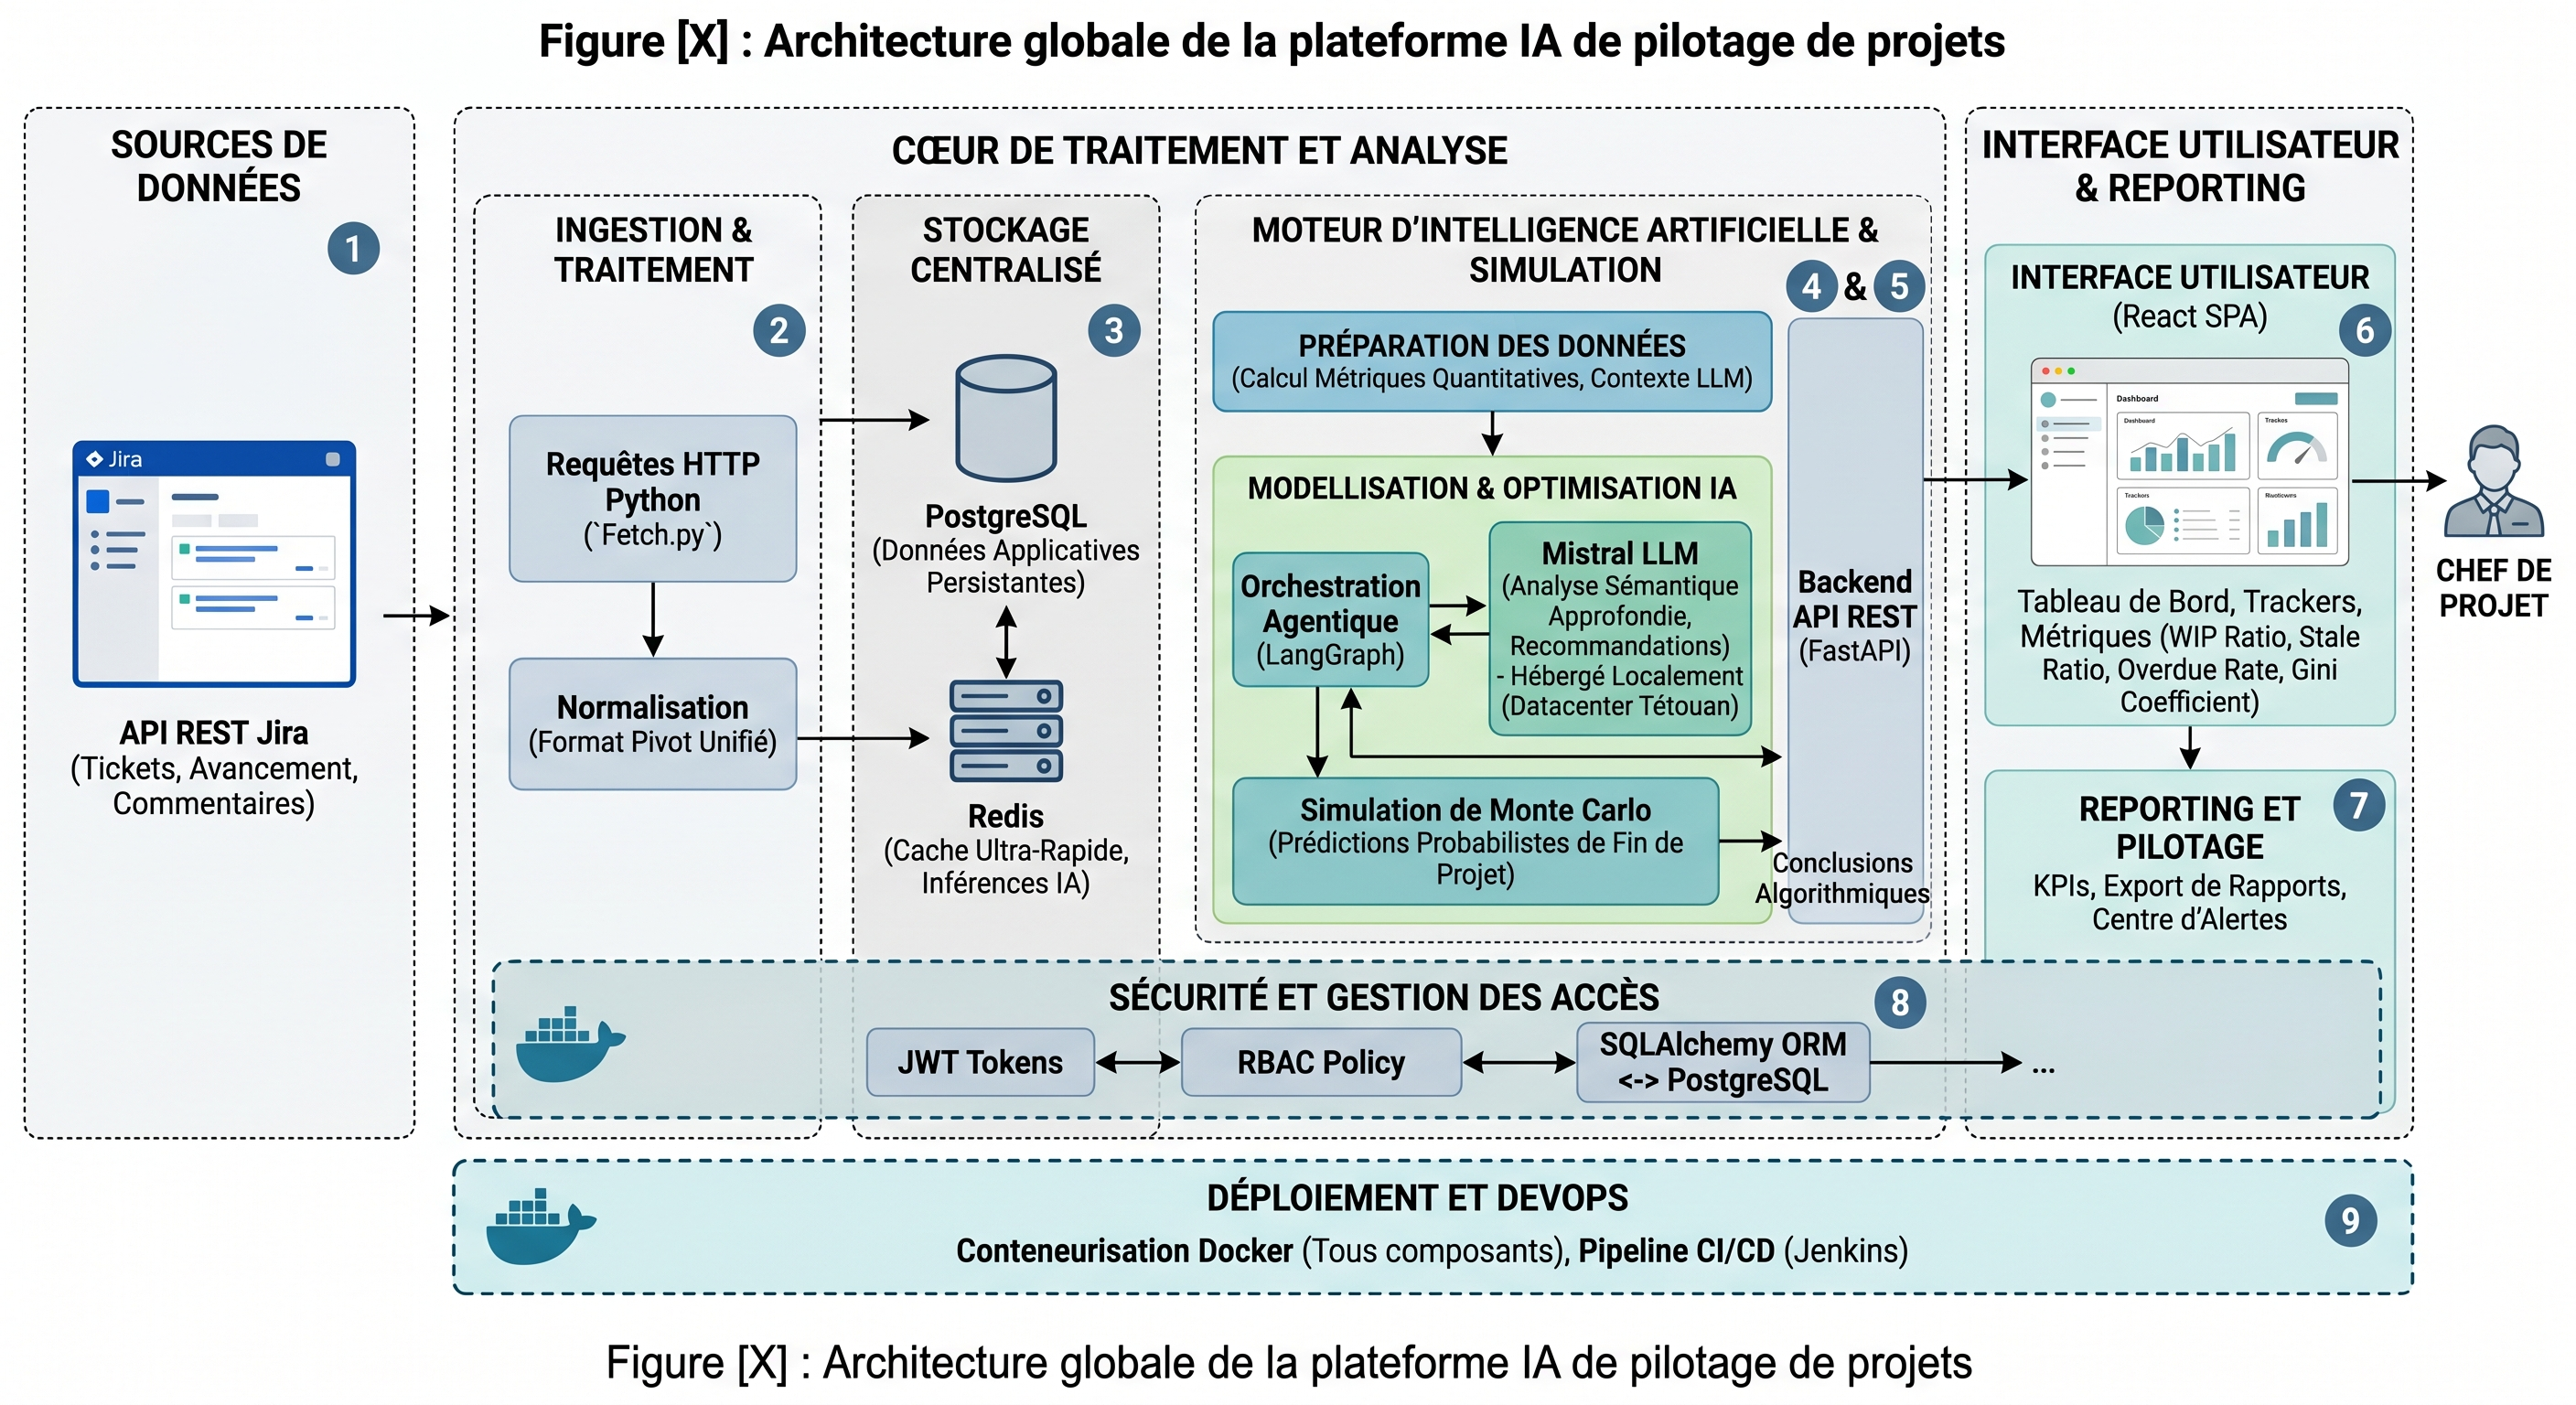
\includegraphics[width=0.9\linewidth]{assets/architecture_globale.png}
\caption{Architecture globale de la plateforme IA de pilotage de projets}
\label{fig:archi_globale}
\end{figure}

L'architecture se compose des éléments suivants :
\begin{enumerate}
\item \textbf{Sources de données :} L'application interagit en premier lieu avec l'API REST de Jira. Cette interface constitue la source de vérité externe, fournissant l'exhaustivité des informations relatives à la gestion de projet (détail des tickets, statuts d'avancement, assignations, historiques de transition et commentaires).
\item \textbf{Ingestion et traitement des données :} La récupération des données brutes est assurée de manière programmatique via des requêtes HTTP en Python. Des modules spécifiques de service (notamment \texttt{Fetch.py}) se chargent ensuite de la normalisation, transformant les structures JSON hétérogènes renvoyées par Jira en un format unifié et exploitable par le cœur de calcul.
\item \textbf{Stockage centralisé :} La persistance des données repose sur une double infrastructure. Une base de données relationnelle PostgreSQL est utilisée pour le stockage persistant et sécurisé des données applicatives (informations utilisateurs, rôles, configurations). En parallèle, un système en mémoire Redis est déployé en tant que cache ultra-rapide pour stocker les calculs statistiques et les inférences de l'IA, évitant ainsi la latence des recalculs.
\item \textbf{Moteur d'intelligence artificielle :} Véritable cerveau du système, ce moteur associe un système de règles déterministes à une approche agentique orchestrée par le framework LangGraph. L'analyse sémantique approfondie est déléguée au modèle de langage large (LLM) Mistral. Pour des raisons strictes de conformité et de protection des données, ce modèle est physiquement hébergé sur les serveurs locaux de NTT DATA au datacenter de Tétouan.
\item \textbf{Moteur de simulation :} Afin d'apporter une dimension prédictive au suivi, un moteur de simulation de Monte Carlo est implémenté en Python, tirant parti de bibliothèques de calcul scientifique telles que NumPy et Pandas. Ce moteur génère des scénarios probabilistes basés sur les durées historiques des tâches pour anticiper de manière réaliste la date d'achèvement d'un projet.
\item \textbf{Interface utilisateur :} L'interaction avec le chef de projet est matérialisée par une application web dynamique (Single Page Application) construite avec la bibliothèque React. Elle héberge le tableau de bord principal et des explorateurs spécifiques, affichant en temps réel des métriques avancées telles que le ratio des travaux en cours (WIP ratio), le taux de tickets obsolètes (stale ratio), le taux de retard (overdue rate) et le coefficient d'inégalité de Gini.
\item \textbf{Reporting et pilotage :} Le tableau de bord agit comme la tour de contrôle du projet en agrégeant les indicateurs de performance clés (KPI) au sein de grilles graphiques et de diagrammes. Il intègre un système de boutons d'exportation pour le reporting de direction, ainsi qu'un centre d'alertes affichant directement les recommandations de l'IA.
\item \textbf{Sécurité et gestion des accès :} La sécurisation des points de terminaison est garantie par un mécanisme de jetons JSON Web Tokens (JWT). Une politique stricte de contrôle d'accès basé sur les rôles (RBAC) est mise en place, avec un mappage des droits géré par l'ORM SQLAlchemy communiquant avec la base PostgreSQL.
\item \textbf{Déploiement et DevOps :} Afin d'assurer une reproductibilité sans faille entre le développement et l'infrastructure client, l'ensemble des composants (frontend, backend FastAPI, bases de données) est encapsulé dans des conteneurs Docker. Le cycle de livraison est orchestré par un pipeline d'intégration et de déploiement continus (CI/CD) opéré sous Jenkins.
\end{enumerate}

\subsection{Zoom sur l'architecture du module d'intelligence artificielle}
Le module d'intelligence artificielle constitue le noyau prédictif et qualitatif de la plateforme. Conçu pour dépasser la simple agrégation statistique, il agit comme un véritable agent expert autonome, capable de déduire des risques systémiques en croisant des données mathématiques avec des nuances sémantiques. L'intégration de LangGraph permet spécifiquement de maintenir l'état conversationnel de l'agent, lui conférant une « mémoire » de sa chaîne de raisonnement à travers les différentes étapes de l'analyse.
\begin{figure}[H]
\centering
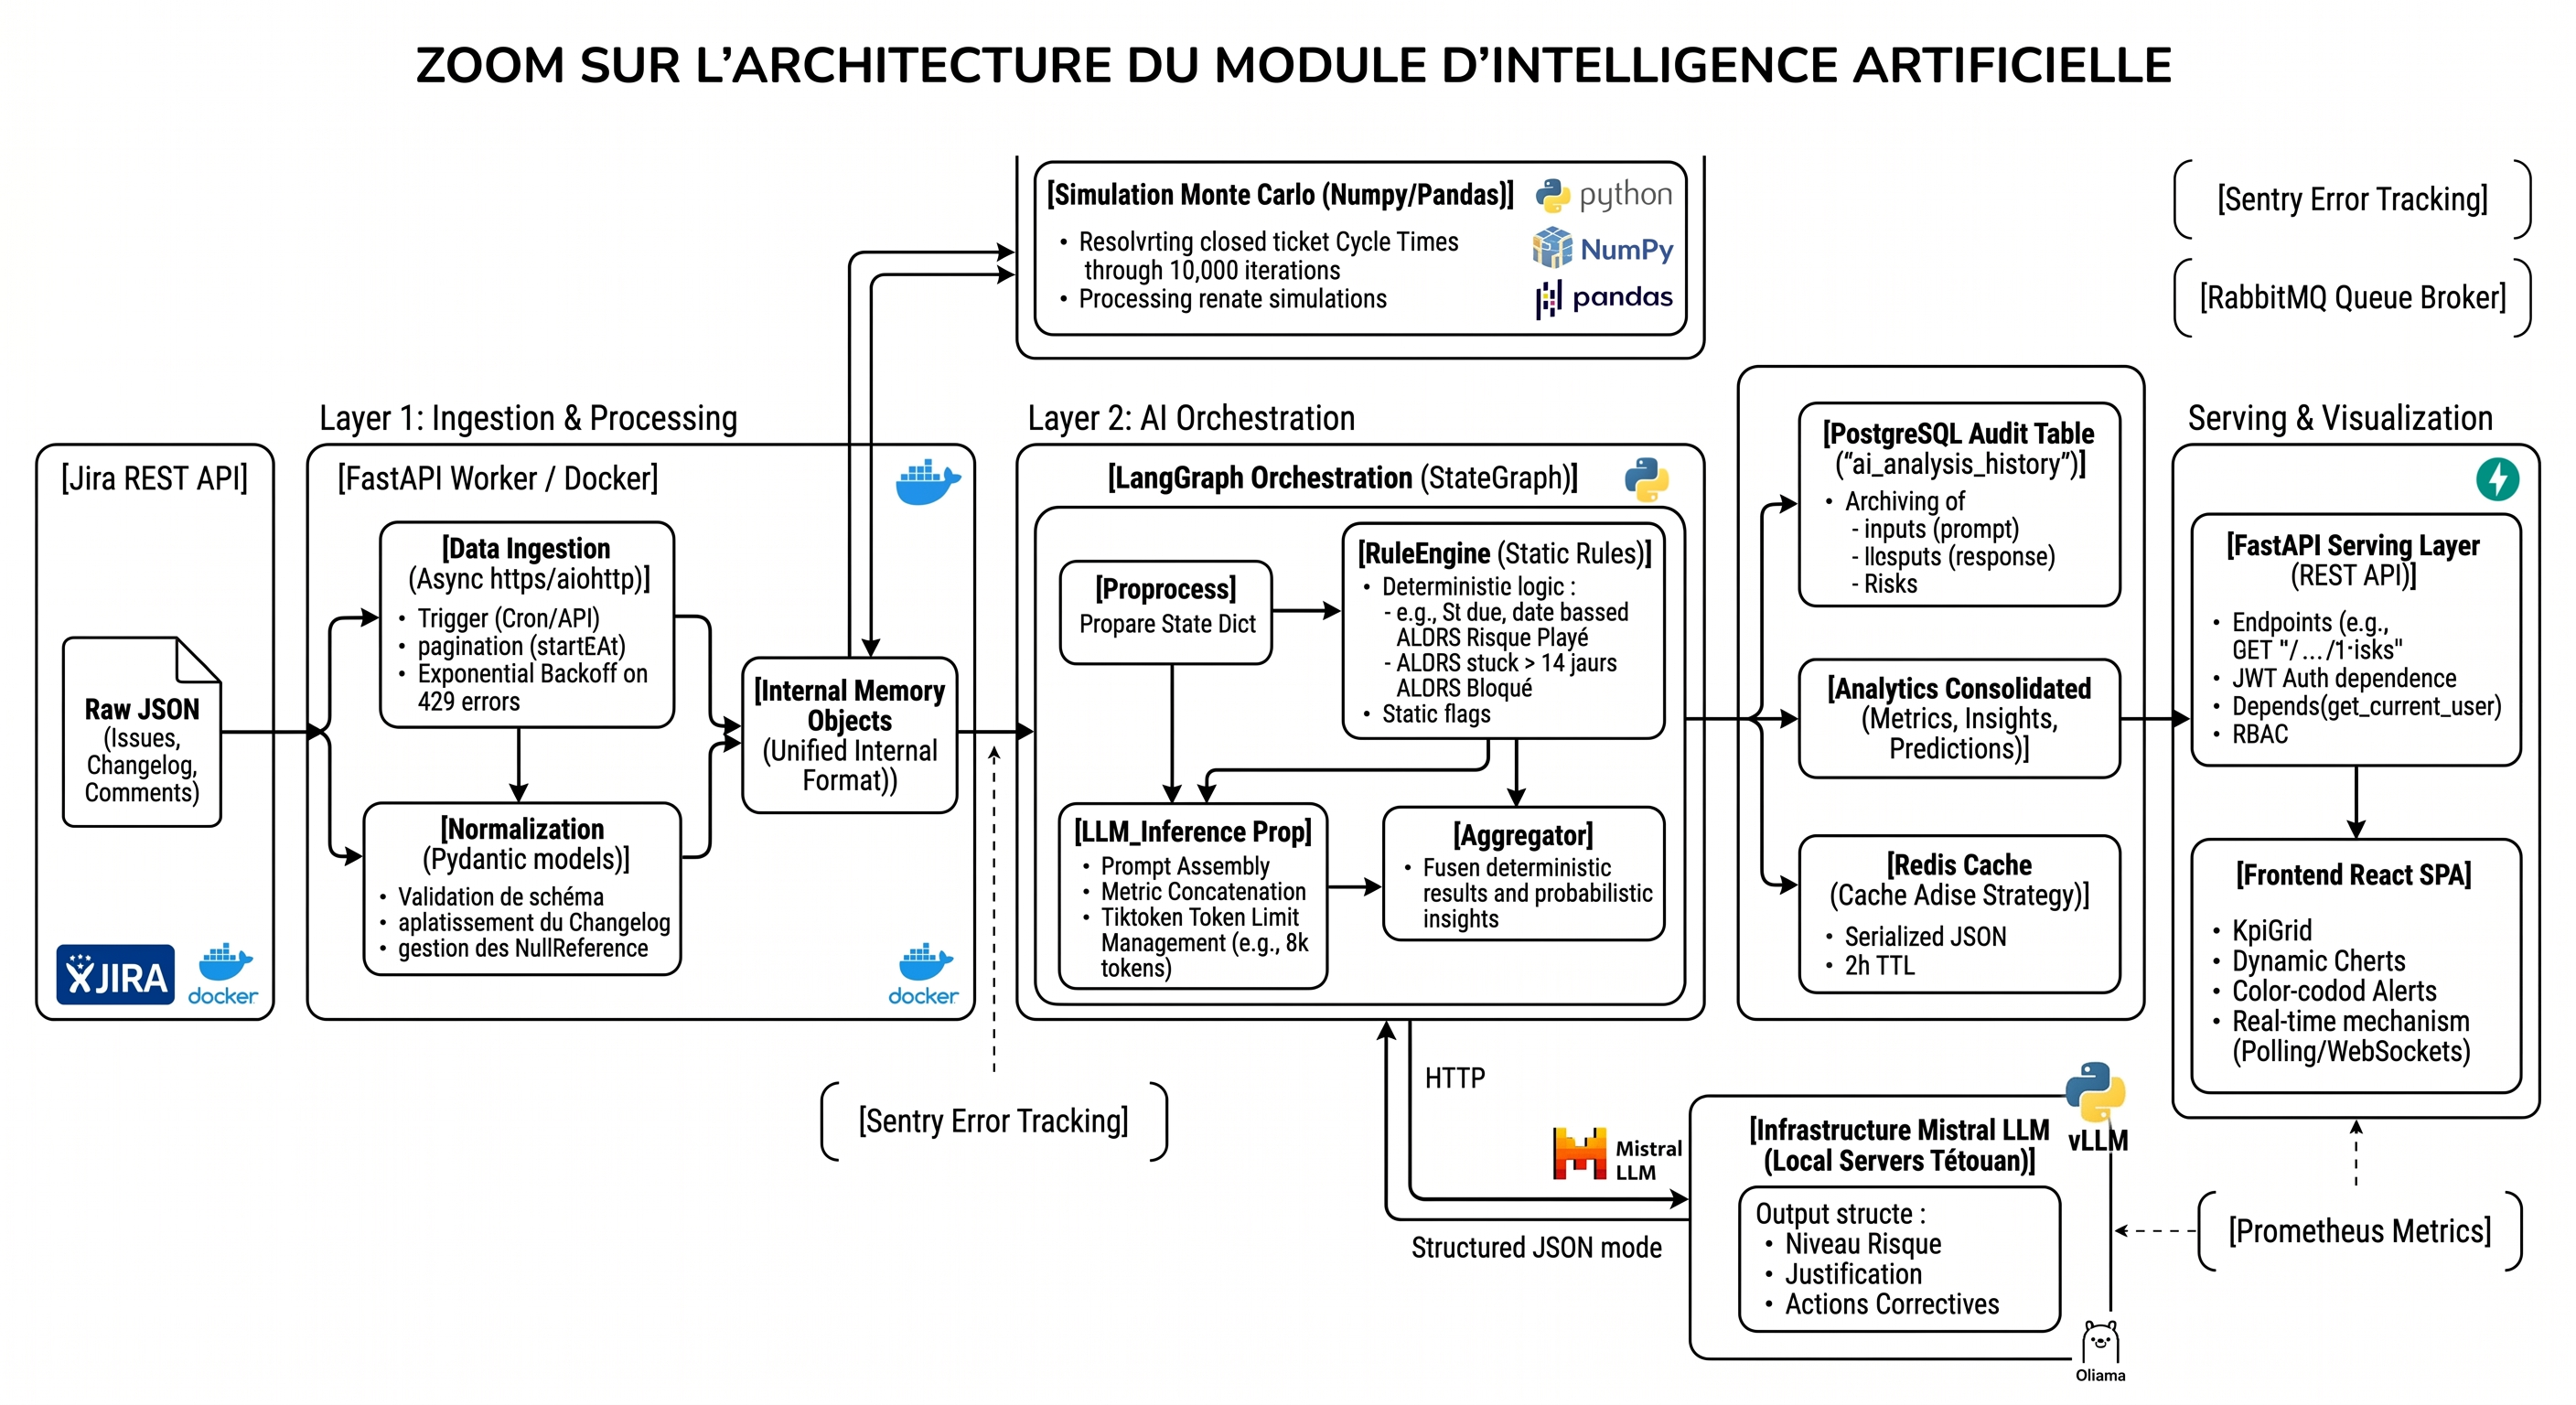
\includegraphics[width=0.9\linewidth]{assets/architecture_ai.png}
\caption{Architecture globale de IA}
\label{fig:archi_ai}
\end{figure}


L'architecture de ce module suit un pipeline structuré en plusieurs phases :
\begin{enumerate}
\item \textbf{Prétraitement et préparation des données}
\begin{itemize}
\renewcommand{\labelitemi}{—}
    \item Extraction asynchrone des données de gestion de projet via l'API REST Jira.
    \item Normalisation des champs pour consolider les structures disparates en un format pivot unifié.
    \item Calcul intensif des métriques quantitatives fondamentales (WIP ratio, stale ratio, overdue rate, coefficient de Gini).
    \item Préparation contextuelle des entrées pour le modèle LLM, impliquant l'assemblage cohérent des descriptions de tâches, des commentaires techniques et des historiques d'évolution.
\end{itemize}

\item \textbf{Modélisation et optimisation IA}
\begin{itemize}
\renewcommand{\labelitemi}{—}
    \item Filtrage préalable par un moteur de règles statiques visant à identifier instantanément les risques évidents (délais structurellement dépassés, tickets bloqués).
    \item Orchestration du flux cognitif par LangGraph, qui encadre la logique de décision et gère l'état d'exécution de l'agent.
    \item Soumission des requêtes au LLM Mistral (hébergé en circuit fermé à Tétouan) pour effectuer une analyse sémantique des échanges et générer des recommandations d'actions correctives.
    \item Exécution de la simulation de Monte Carlo pour déduire, à partir de la variance historique, une prédiction probabiliste de la date de fin de projet.
\end{itemize}

\item \textbf{Déploiement via API et conteneurisation}
\begin{itemize}
\renewcommand{\labelitemi}{—}
    \item Exposition unifiée des conclusions algorithmiques (scores de risques, textes de recommandation, intervalles de confiance prédictifs) par l'intermédiaire d'une API REST développée avec le framework asynchrone FastAPI.
    \item Isolation du processus analytique au sein d'un environnement conteneurisé Docker.
\end{itemize}

\item \textbf{Intégration applicative et visualisation}
\begin{itemize}
\renewcommand{\labelitemi}{—}
    \item Transmission asynchrone des résultats d'analyse vers le système de cache Redis, garantissant une mise à disposition véloce au backend.
    \item Restitution visuelle et interprétation dans le tableau de bord React, traduisant les vecteurs de données en éléments d'interface lisibles (alertes, recommandations, graphiques dynamiques).
    \item Maintien d'une traçabilité des décisions algorithmiques et conservation de l'historique des analyses.
\end{itemize}
\end{enumerate}


\section{Environnements logiciels et technologies}
Cette section présente les outils, langages et environnements utilisés au cours du projet, en justifiant les choix technologiques réalisés à chaque étape. Une veille technologique a également été menée dans le cadre de l’exploration des solutions open-source pour l’orchestration d’agents IA et l’hébergement local de modèles de langage.

\subsection{Technologies utilisées}
Afin de mettre en œuvre le projet selon l’architecture définie, nous avons mobilisé plusieurs technologies :

\textbf{Python} — Langage principal utilisé pour le développement du backend et du module d’intelligence artificielle. Python a été choisi pour sa flexibilité, sa lisibilité, ainsi que la richesse de son écosystème scientifique. Les bibliothèques suivantes ont été mobilisées :

\begin{figure}[H]
\centering

\includegraphics[width=0.2\linewidth]{assets/logos/python.png}
\caption{Python}
\label{fig:Python}
\end{figure}

\begin{itemize}
\renewcommand{\labelitemi}{—}
    \item \textbf{FastAPI} : framework asynchrone pour la création d’API RESTful, facilitant l’exposition des services IA et l’intégration avec le frontend React.
    \begin{figure}[H]
    \centering
    
\includegraphics[width=0.2\linewidth]{assets/logos/fastApi.png}
    \caption{Python fast api}
    \label{fig:Python_fastapi}
    \end{figure}
    \item \textbf{SQLAlchemy} : ORM utilisé pour interagir avec la base de données PostgreSQL, permettant une gestion élégante des modèles utilisateurs et des rôles RBAC.
    \begin{figure}[H]
    \centering
    
\includegraphics[width=0.2\linewidth]{assets/logos/sqlalchemy.jpg}
    \caption{sqlalchemy}
    \label{fig:sqlalchemy}
    \end{figure}
    \item \textbf{LangGraph} : framework d’orchestration d’agents IA, retenu pour sa capacité à maintenir un état conversationnel et à gérer des flux de décision cycliques.
    \begin{figure}[H]
    \centering
    
\includegraphics[width=0.2\linewidth]{assets/logos/langgraph.png}
    \caption{Python langgraph}
    \label{fig:Python_langgraph}
    \end{figure}
    \item \textbf{Mistral} : modèle de langage large (LLM) hébergé localement sur les serveurs de Tétouan, choisi pour son équilibre entre performance et confidentialité des données.
    \begin{figure}[H]
    \centering
    
\includegraphics[width=0.2\linewidth]{assets/logos/mistral.jpeg}
    \caption{Python}
    \label{fig:Python_mistral}
    \end{figure}
    \item \textbf{NumPy, Pandas} : bibliothèques de calcul scientifique utilisées pour les simulations de Monte Carlo et le calcul des métriques (WIP ratio, stale ratio, coefficient de Gini).
    \begin{figure}[H]
    \centering
    
\includegraphics[width=0.2\linewidth]{assets/logos/numpy.jpg}
    \caption{Python numpy}
    \label{fig:Python_numpy}
    \end{figure}
\end{itemize}

\textbf{React} — Bibliothèque JavaScript utilisée pour le développement du tableau de bord interactif. React permet une expérience utilisateur réactive et une visualisation en temps réel des métriques et alertes.

\begin{figure}[H]
\centering

\includegraphics[width=0.2\linewidth]{assets/logos/react_logo.png}
\caption{react}
\label{fig:react}
\end{figure}

\textbf{PostgreSQL} — Système de gestion de base de données relationnelle, retenu pour sa robustesse et sa conformité aux exigences de sécurité (stockage des identifiants, rôles et configurations).

\begin{figure}[H]
\centering

\includegraphics[width=0.3\linewidth]{assets/logos/postgres_logo.png}
\caption{postgres}
\label{fig:postgres}
\end{figure}

\textbf{Redis} — Système de cache en mémoire déployé pour accélérer l’accès aux résultats des analyses IA et aux métriques fréquemment sollicitées, réduisant ainsi la latence du tableau de bord.

\begin{figure}[H]
\centering

\includegraphics[width=0.2\linewidth]{assets/logos/redis.png}
\caption{redis}
\label{fig:redis}
\end{figure}

\textbf{Docker} — Outil de conteneurisation permettant d’encapsuler l’ensemble des composants (backend FastAPI, frontend React, base de données) dans des environnements isolés et reproductibles.

\begin{figure}[H]
\centering

\includegraphics[width=0.2\linewidth]{assets/logos/docker.png}
\caption{docker}
\label{fig:docker}
\end{figure}

\textbf{Jenkins} — Serveur d’intégration continue utilisé pour automatiser les pipelines CI/CD, assurant les tests, la construction et le déploiement de la plateforme.
\begin{figure}[H]
\centering

\includegraphics[width=0.4\linewidth]{assets/logos/jenkins.jpg}
\caption{jenkins}
\label{fig:jenkins}
\end{figure}

\subsection{Technologies utilisées par l’équipe de développement}
L’équipe de développement a utilisé un ensemble d’outils collaboratifs et d’environnements de travail :
\begin{itemize}
\renewcommand{\labelitemi}{—}
    \item \textbf{Visual Studio Code} : IDE principal, apprécié pour ses extensions Python, son débogueur intégré et son terminal facilitant les tests.
    \begin{figure}[H]
    \centering
    
\includegraphics[width=0.2\linewidth]{assets/logos/vsCode.png}
    \caption{vs}
    \label{vs}
    \end{figure}
    \item \textbf{GitLab} : plateforme de gestion de version basée sur Git, utilisée pour le suivi des modifications du code source et la collaboration entre développeurs, accessible à l’adresse \href{https://umane.emeal.nttdata.com/git/FELTRIINTPROJ/nttdata-ai-agent-project-tracking}{https://umane.emeal.nttdata.com/git/FELTRIINTPROJ/nttdata-ai-agent-project-tracking}.    \item \textbf{Microsoft Teams} : outil de communication quotidienne pour les réunions de synchronisation (daily stand-ups) et les échanges avec l’encadrement.
    \begin{figure}[H]
    \centering
    
\includegraphics[width=0.2\linewidth]{assets/logos/gitlab_logo.png}
    \caption{gitlab}
    \label{fig:gitlab}
    \end{figure}
    \item \textbf{Jira} : utilisé pour le suivi des tâches du projet lui-même, accessible à l’adresse \href{https://umane.emeal.nttdata.com/jiraito/browse/HPCMOROCCO}{https://umane.emeal.nttdata.com/jiraito/browse/HPCMOROCCO}, démontrant ainsi l’adéquation de la plateforme avec les méthodes agiles.    \item \textbf{Postman} : outil de test d’API REST, employé pour valider les endpoints FastAPI avant intégration.
    \begin{figure}[H]
    \centering
    
\includegraphics[width=0.2\linewidth]{assets/logos/jira_logo.png}
    \caption{jira}
    \label{fig:jira}
    \end{figure}
    \item \textbf{Docker Compose} : utilisé en développement pour orchestrer l’exécution simultanée des conteneurs backend, frontend, PostgreSQL et Redis.
    \begin{figure}[H]
    \centering
    
\includegraphics[width=0.2\linewidth]{assets/logos/docker.png}
    \caption{docker}
    \label{fig:docker}
    \end{figure}
\end{itemize}

\subsection{Veille technologique sur les agents IA conversationnels pour l’analyse de projets}
Dans le cadre de l’exploration des solutions open-source pour l’analyse automatisée des risques à partir de données Jira, une veille technologique a été menée. Plusieurs technologies ont été examinées :
\begin{itemize}
\renewcommand{\labelitemi}{—}
    \item \textbf{LangChain} : framework populaire pour la construction d’applications LLM, mais moins adapté aux graphes d’état complexes.
    \begin{figure}[H]
    \centering
    
\includegraphics[width=0.2\linewidth]{assets/logos/langchain.png}
    \caption{langchain}
    \label{fig:langchain}
    \end{figure}
    \item \textbf{LlamaIndex} : spécialisé dans l’indexation et la récupération de documents, sans capacité native d’orchestration d’agents.
    \begin{figure}[H]
    \centering
    
\includegraphics[width=0.2\linewidth]{assets/logos/llamaindex_logo.png}
    \caption{llama}
    \label{fig:llama}
    \end{figure}
    \item \textbf{Rasa} : conçu pour les chatbots conversationnels, mais trop lourd et non orienté vers l’analyse de données structurées de gestion de projet.
    \begin{figure}[H]
    \centering
    
\includegraphics[width=0.2\linewidth]{assets/logos/rasa_logo.png}
    \caption{rasa}
    \label{fig:rasa}
    \end{figure}
    \item \textbf{Mistral vs. LLaMA 3} : comparaison de modèles de langage open-source pouvant être hébergés localement.
    \begin{figure}[H]
    \centering
    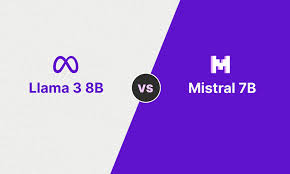
\includegraphics[width=0.2\linewidth]{assets/logos/llama_mistral.jpg}
    \caption{llama_index}
    \label{fig:llama_index}
    \end{figure}
\end{itemize}
À l’issue de cette veille, \textbf{LangGraph} a été retenu pour l’orchestration de l’agent IA, et \textbf{Mistral} pour le LLM, en raison de sa faible empreinte mémoire et de son excellente gestion de la langue française.

\subsection{Comparaison des outils d’orchestration d’agents IA}
Le tableau \ref{tab:comparaison_orchestration} présente une comparaison synthétique entre deux frameworks d’orchestration envisagés : LangChain et LangGraph.

\begin{table}[H]
\centering
\renewcommand{\arraystretch}{1.2}
\caption{Comparaison entre LangChain et LangGraph}
\begin{tabular}{|l|l|l|}
\hline
\textbf{Critère} & \textbf{LangChain} & \textbf{LangGraph} \\
\hline
Nature & Chaînes linéaires & Graphes d’état cycliques \\
Gestion de la mémoire & Limitée (contextuelle) & Native (état persistant) \\
Adaptation aux agents autonomes & Modérée & Excellente \\
Cycles et boucles de décision & Non supporté & Supporté nativement \\
Courbe d’apprentissage & Faible à modérée & Modérée \\
Intégration avec FastAPI & Bonne & Très bonne \\
\hline
\end{tabular}
\label{tab:comparaison_orchestration}
\end{table}

La comparaison montre que LangGraph, bien qu’étant plus récent, est mieux adapté à notre besoin d’un agent conversationnel autonome capable de maintenir un état de raisonnement sur plusieurs cycles d’analyse. LangGraph a donc été retenu pour le développement du module IA.

\subsection{Conclusion}
Ce chapitre a présenté la conception fonctionnelle et technique de notre solution, en partant de l’analyse des besoins jusqu’au choix des technologies. Nous avons détaillé l’architecture globale du système ainsi que celle du module d’intelligence artificielle. Une étude comparative des outils d’orchestration d’agents IA a également permis de justifier les choix technologiques retenus.

Le chapitre suivant portera sur l’implémentation détaillée de la plateforme, décrivant les algorithmes mis en œuvre, l’intégration des composants, ainsi que les résultats obtenus lors des phases de test et de validation.
	\chapter{Description des données}
\label{ch:description_donnees}

\section{Introduction}
Ce chapitre est consacré à la description approfondie du cycle de vie des données au sein de notre plateforme d’analyse de risques basée sur l’intelligence artificielle. La performance des algorithmes de détection de risques, de l’agent conversationnel (LangGraph + Mistral) et des simulations prédictives (Monte Carlo) dépend directement de la qualité, de la structure et de la fraîcheur des données extraites de l’écosystème Jira de NTT DATA Maroc. Nous détaillons d’abord les sources et les méthodes d’extraction des données, puis leur structure interne. Ensuite, nous présentons les analyses et visualisations clés qui alimentent le tableau de bord React. Enfin, nous décrivons le pipeline de normalisation et de préparation qui transforme les flux JSON bruts en signaux standardisés prêts à être consommés par les moteurs d’IA et de simulation.

\section{Source des données}
La source primaire et unique de notre plateforme est l’API REST de Jira (version 2), qui expose l’intégralité des données opérationnelles des projets logiciels suivis par NTT DATA Maroc. L’extraction est conçue pour être résiliente, asynchrone et respectueuse des limites de débit imposées par Jira.

\subsection{Authentification et endpoints utilisés}
L’accès à l’API est sécurisé par des sessions HTTP basées sur des jetons d’authentification (Basic Auth ou token personnel). Les principaux endpoints exploités sont :

\begin{figure}[H]
\centering
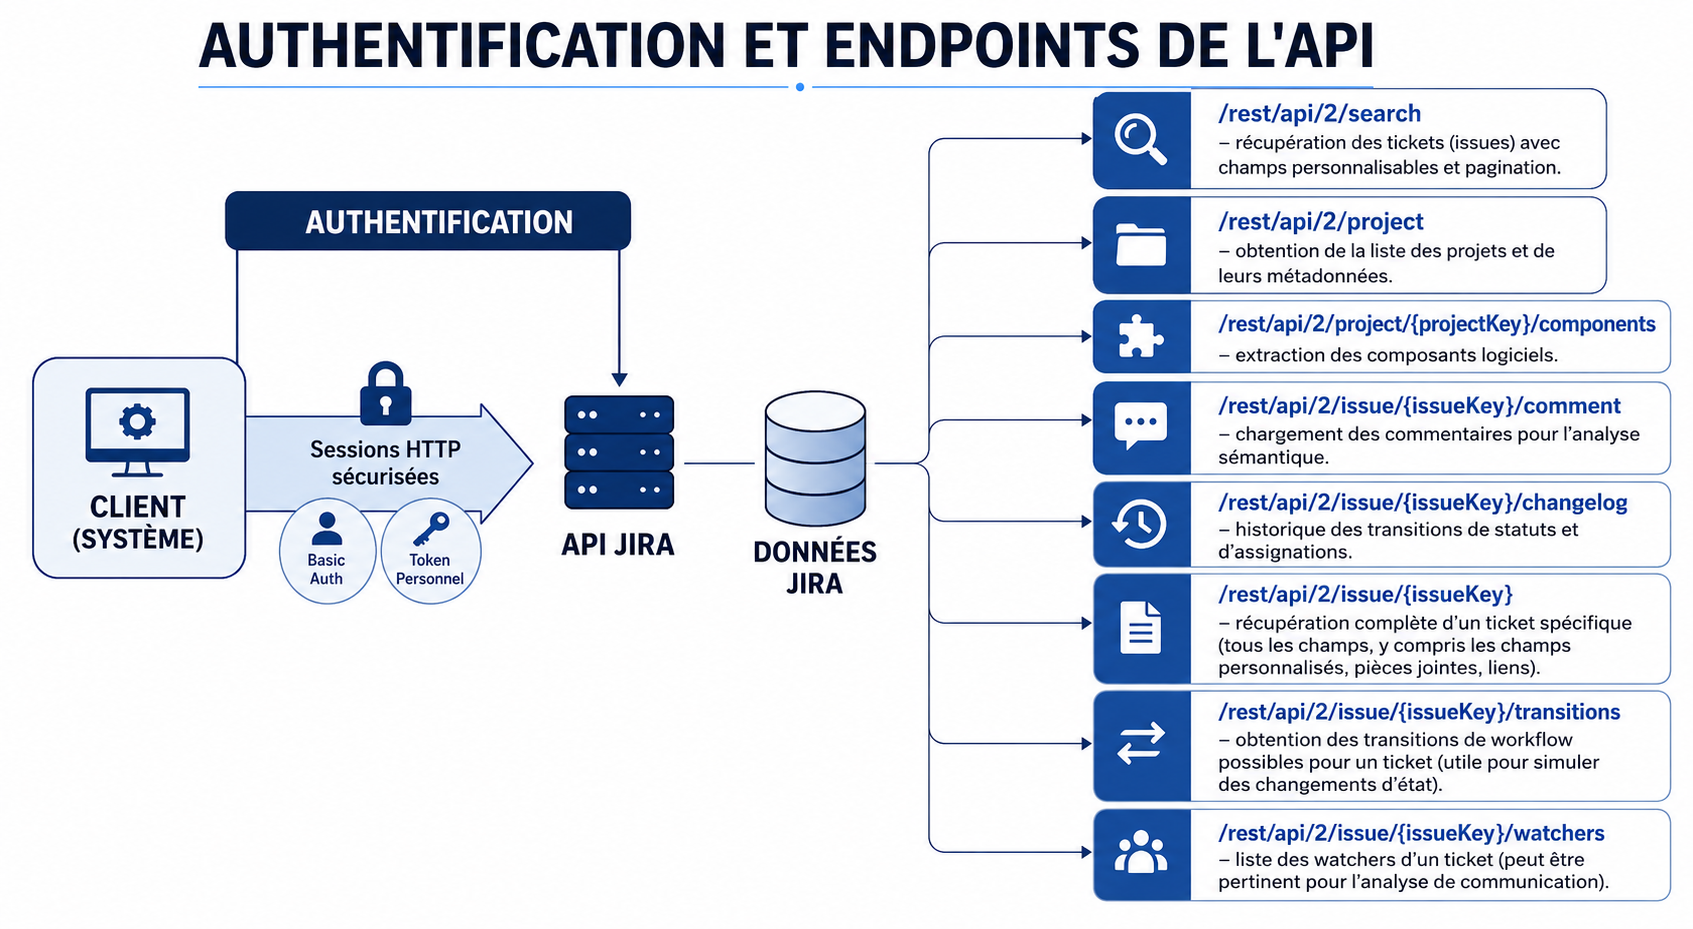
\includegraphics[width=0.9\linewidth]{assets/sourceD_authentification.png}
\caption{Schéma du mécanisme d’authentification à l’API Jira}
\label{fig:authentification}
\end{figure}    

\begin{itemize}
    \renewcommand{\labelitemi}{—}
    \item \texttt{/rest/api/2/search} : récupération des tickets (issues) avec champs personnalisables et pagination.
    \item \texttt{/rest/api/2/project} : obtention de la liste des projets et de leurs métadonnées.
    \item \texttt{/rest/api/2/project/\{projectKey\}/components} : extraction des composants logiciels.
    \item \texttt{/rest/api/2/issue/\{issueKey\}/comment} : chargement des commentaires pour l’analyse sémantique.
    \item \texttt{/rest/api/2/issue/\{issueKey\}/changelog} : historique des transitions de statuts et d’assignations.
    \item \texttt{/rest/api/2/issue/\{issueKey\}} : récupération complète d’un ticket spécifique (tous les champs, y compris les champs personnalisés, pièces jointes, liens).
    \item \texttt{/rest/api/2/issue/\{issueKey\}/transitions} : obtention des transitions de workflow possibles pour un ticket (utile pour simuler des changements d’état).
    \item \texttt{/rest/api/2/issue/\{issueKey\}/watchers} : liste des watchers d’un ticket (peut être pertinent pour l’analyse de communication).
\end{itemize}

\subsection{Requêtes JQL (Jira Query Language)}

Le \textbf{Jira Query Language (JQL)} est un langage de requête structuré propre à Jira Data Center, conçu pour interroger la base de données des tickets, projets, commentaires et historiques. Il permet de filtrer, trier et extraire uniquement les informations pertinentes selon des critères métiers précis (projet, dates, statuts, priorités, etc.). L’utilisation de JQL est essentielle pour limiter la charge sur l’API et ne conserver que les données nécessaires aux calculs de métriques et à l’entraînement de l’agent IA.

\paragraph{Bénéfices de l’utilisation de JQL dans notre plateforme}
\begin{itemize}
    \renewcommand{\labelitemi}{—}
    \item Réduction du volume de données transférées (seules les issues répondant aux critères temporels sont extraites).
    \item Amélioration des performances : les requêtes paginées sont exécutées plus rapidement grâce à des index optimisés par Jira.
    \item Flexibilité : adaptation dynamique des requêtes selon le contexte (analyse temps réel vs historique Monte Carlo).
    \item Respect des quotas de l’API (rate limiting) en limitant le nombre de tickets chargés.
\end{itemize}

\paragraph{Architecture de l’intégration des requêtes JQL dans l’application}

La figure \ref{fig:architecture_jql} illustre l’architecture d’intégration des requêtes JQL dans le backend FastAPI.
\begin{figure}[H]
\centering
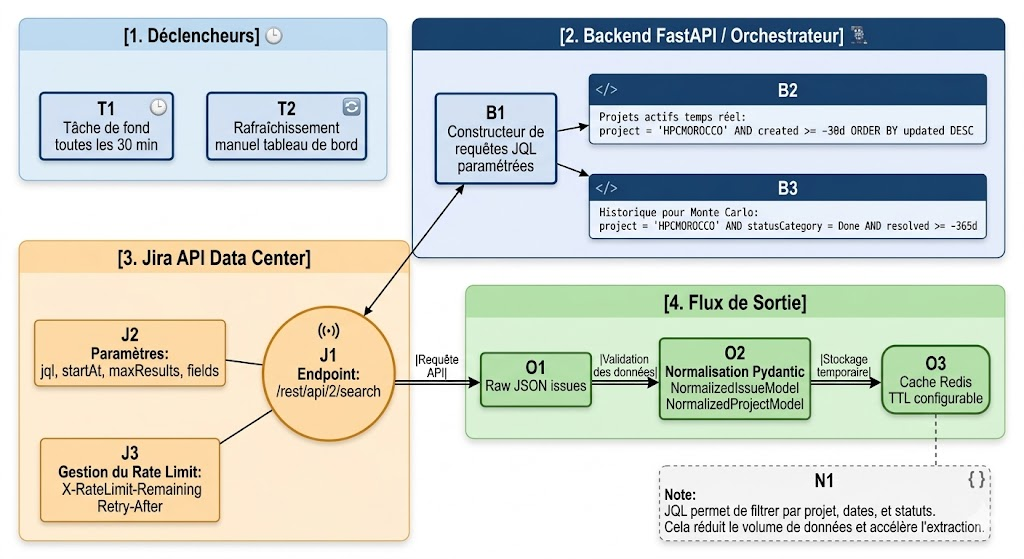
\includegraphics[width=0.9\linewidth]{assets/diagrams/arch_jql.jpg}
\caption{Intégration des requêtes JQL dans le backend FastAPI (architecture)}
\label{fig:architecture_jql}
\end{figure} 

La construction et l’exécution des requêtes JQL sont orchestrées par le backend FastAPI. Deux mécanismes de déclenchement sont mis en œuvre :
\begin{itemize}
    \renewcommand{\labelitemi}{—}
    \item \textbf{Tâche de fond} : toutes les 30 minutes, une routine asynchrone exécute une série de requêtes JQL prédéfinies (ex. historique des 365 derniers jours) pour maintenir le cache Redis à jour.
    \item \textbf{Requête à la demande} : lorsqu’un utilisateur rafraîchit le tableau de bord, le backend construit dynamiquement la requête JQL correspondant au projet sélectionné et aux filtres actifs (ex. “created >= -30d” pour les tickets récents).
\end{itemize}
Les requêtes sont paramétrées pour éviter les injections et garantissent la pagination automatique via \texttt{startAt} et \texttt{maxResults}. Les exemples suivants illustrent les deux cas d’usage principaux.

\paragraph{Exemples de requêtes utilisées}
Pour l’analyse temps réel des projets actifs :
\begin{verbatim}
project = "HPCMOROCCO" AND created >= -30d ORDER BY updated DESC
\end{verbatim}
Pour l’historique nécessaire aux simulations de Monte Carlo (vélocité) :
\begin{verbatim}
project = "HPCMOROCCO" AND statusCategory = Done AND resolved >= -365d
\end{verbatim}

Ces requêtes sont exécutées soit périodiquement par la tâche de fond, soit à la demande lors du rafraîchissement de l’interface.

\subsection{Gestion des limites de taux et optimisation}
L’API Jira impose des quotas stricts (ex. 100 requêtes par minute). Notre module \texttt{Fetch.py} implémente les mécanismes suivants :
\begin{itemize}
    \renewcommand{\labelitemi}{—}
    \item Détection des en‑têtes \texttt{X-RateLimit-Remaining} et \texttt{Retry-After}.
    \item Backoff exponentiel avec temporisation progressive en cas de réponse HTTP 429 (trop de requêtes) ou 503 (service indisponible).
    \item Parallélisation contrôlée par \texttt{ThreadPoolExecutor} pour les lots de tickets (batch de 200, soit 2 pages de 100), sans dépasser les limites.
\end{itemize}
La mise en cache des résultats est détaillée dans la section dédiée au stockage (cf. \ref{subsec:stockage_cache}).

\section{Description des données}
Les données brutes retournées par Jira sont au format JSON, riches mais hétérogènes. Le schéma standard de l’API Jira v2 structure l’information de la manière suivante : l’objet racine contient les métadonnées du ticket (clé, URL, etc.), et l’ensemble des champs métier est regroupé dans un objet \texttt{fields}. L’historique des transitions (\texttt{changelog}) est récupéré via un endpoint dédié et contient une liste d’entrées \texttt{histories}, chacune composée d’un timestamp et d’une liste d’items (\texttt{items}) décrivant les changements de champ.






\subsection{Champs des tickets (issues)}

La figure \ref{fig:jira_json_structure} présente un extrait d’un ticket Jira tel qu’il est retourné par l’API, mettant en évidence la structure imbriquée des champs.


\begin{figure}[H]
\centering
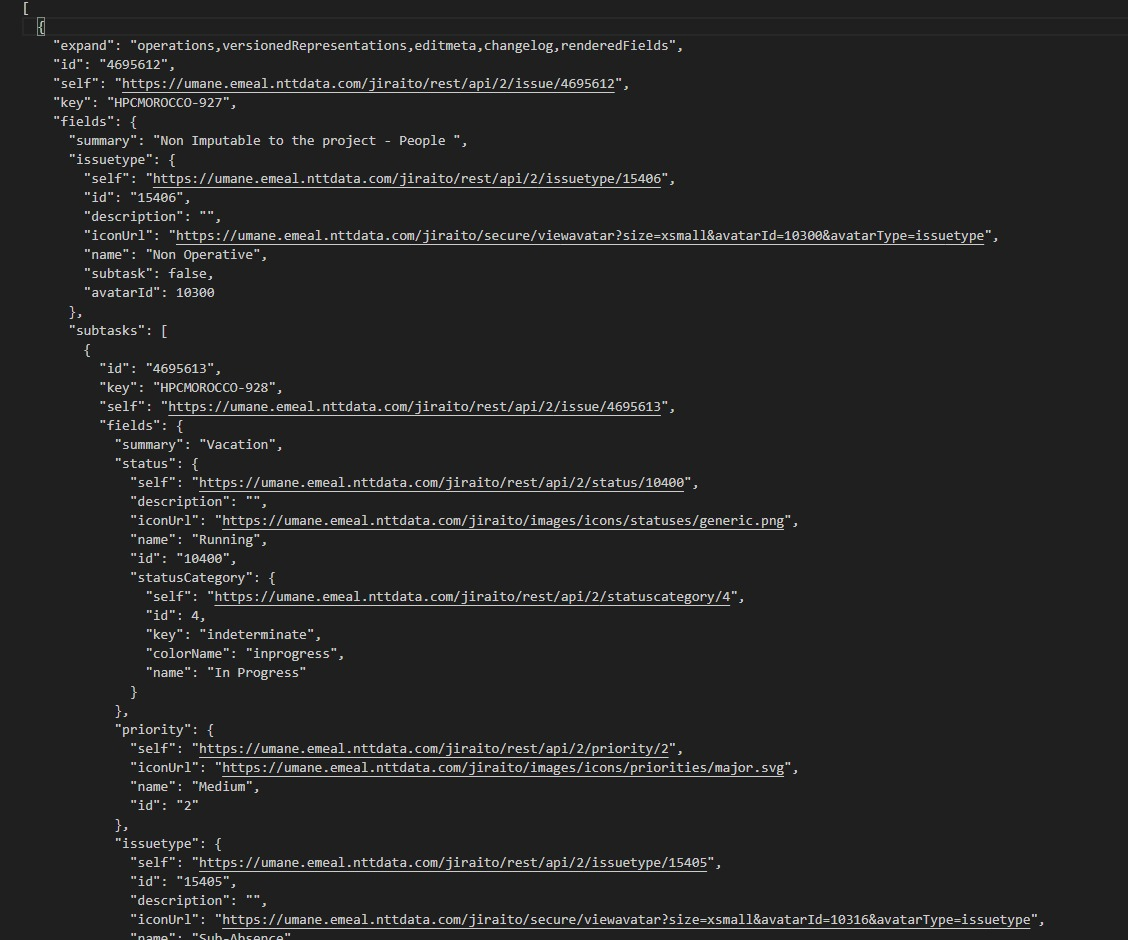
\includegraphics[width=0.9\linewidth]{assets/interfaces/json_screen.jpeg}
\caption{Extrait d’un ticket Jira au format JSON (structure imbriquée \texttt{fields}, \texttt{subtasks}, \texttt{statusCategory}, etc.)}
\label{fig:jira_json_structure}
\end{figure}
Chaque ticket est représenté par un objet contenant les champs suivants, sélectionnés pour leur pertinence dans les calculs métier et l’inférence IA :
\begin{itemize}
    \renewcommand{\labelitemi}{—}
    \item \textbf{Identité} : clé (ex. \texttt{HPCMOROCCO-123}), URL, résumé (\texttt{summary}), description (\texttt{description}).
    \item \textbf{Statut et typologie} : statut courant (\texttt{status}), catégorie de statut (\texttt{statusCategory} : \texttt{To Do}, \texttt{In Progress}, \texttt{Done}) permettant la normalisation des états pour le calcul du WIP ratio, type de ticket (\texttt{issuetype} : Bug, Tâche, Story, Épopée), priorité (\texttt{priority}).
    \item \textbf{Liens et dépendances} : champ \texttt{issuelinks} (bloque, est bloqué par, dépend de, etc.), essentiel pour la détection des risques en cascade et des tickets bloqués.
    \item \textbf{Dates} : création (\texttt{created}), dernière mise à jour (\texttt{updated}), échéance (\texttt{duedate}), résolution (\texttt{resolutiondate}).
    \item \textbf{Assignation} : assigné (\texttt{assignee}) avec son \texttt{accountId}, \texttt{displayName} et \texttt{avatarUrl} (exploités par le module Worker Insights pour identifier et visualiser les développeurs), rapporteur (\texttt{reporter}).
    \item \textbf{Estimations et charges} : estimation initiale (\texttt{timeoriginalestimate}), temps restant (\texttt{timeestimate}), temps passé (\texttt{timespent}), et Story Points (champ personnalisé \texttt{customfield\_10016}). Ce champ stocke la complexité estimée des tickets et est utilisé pour les calculs de vélocité et les simulations Monte Carlo.
    \item \textbf{Sprints} : champ personnalisé (ex. \texttt{customfield\_10020}) contenant les informations de sprint (nom, dates de début et de fin). Ce champ permet de regrouper les tickets par itération pour l’analyse de vélocité historique et le suivi de l’avancement agile.
    \item \textbf{Composants et versions} : liste des composants logiciels, versions d’affectation et de correction.
\end{itemize}

\subsection{Commentaires et historique}
L’analyse sémantique (risques cachés, blocages implicites) nécessite l’accès aux commentaires et aux changements d’état. Nous récupérons pour chaque ticket :
\begin{itemize}
    \renewcommand{\labelitemi}{—}
    \item \textbf{Commentaires} : auteur, date, contenu textuel.
    \item \textbf{Changelog} : chaque transition (\texttt{status}, \texttt{assignee}, \texttt{resolution}) avec ancienne valeur, nouvelle valeur et date de changement.
\end{itemize}
Ces données sont conservées sous forme de listes associées au ticket. Le \textit{changelog} est ensuite aplati pour extraire la date de dernière transition et calculer le temps passé dans chaque statut (cycle time), comme détaillé dans la section \ref{subsec:normalisation}.

\subsection{Métadonnées de projet}
Les informations générales sur les projets (clé, nom, catégorie, lead, type) sont stockées séparément pour enrichir les analyses contextuelles. Elles sont conservées dans le cache Redis et rafraîchies périodiquement.

\subsection{Volumétrie et pagination}
Un projet actif de taille moyenne chez NTT DATA peut contenir plusieurs milliers de tickets. Pour éviter les limites de pagination de l’API Jira (50 ou 100 résultats par appel), nous utilisons la pagination basée sur le champ \texttt{startAt} avec une taille de page fixée à 100 tickets. Les appels sont parallélisés par lots de 2 pages consécutives (soit 200 tickets par lot) afin d’accélérer l’extraction de l’historique complet (par exemple, sur une fenêtre de 365 jours) en moins de 30 secondes.

\section{Analyse et Visualisation des Données}
Notre plateforme ne se limite pas à un affichage brut ; elle transforme les données Jira en indicateurs d’aide à la décision (KPI), en alertes de risque et en prévisions. Les visualisations sont intégrées au tableau de bord React à l’aide de bibliothèques comme Recharts ou Plotly.

\subsection{Analyse prédictive par Monte Carlo}
\label{subsec:montecarlo_visu}
La simulation Monte Carlo est utilisée pour prévoir la date de fin du projet en fonction du backlog restant et de la vélocité historique. Le processus est le suivant :
\begin{enumerate}
    \item Extraction des tickets résolus sur les 365 derniers jours.
    \item Calcul de la vélocité hebdomadaire (nombre de tickets clôturés par semaine). On obtient une distribution empirique.
    \item Comptage du nombre de tickets actuellement ouverts (non résolus).
    \item Simulation de 10\,000 scénarios : chaque semaine, on tire aléatoirement une vélocité dans la distribution historique, on soustrait le backlog jusqu’à ce qu’il soit nul.
    \item On extrait les percentiles (p50, p75, p85, p95) des dates de fin obtenues.
\end{enumerate}
L’interface affiche une courbe de probabilité cumulée et un intervalle de confiance. Par exemple, pour le projet pilote \texttt{HPCMOROCCO}, la simulation indique qu’il y a \textbf{90\,\% de chances} que le projet soit terminé avant le 15 décembre, et \textbf{85\,\% de chances} avant le 10 décembre (intervalle p85). Les percentiles p50, p75, p85 et p95 sont également affichés sous forme de repères sur la courbe.

\subsection{Visualisation des métriques de santé projet}
Les métriques de santé projet (WIP ratio, stale ratio, overdue rate, coefficient de Gini) sont calculées en temps réel (leur définition et leur évaluation sont détaillées dans le chapitre 4). Elles sont affichées sous forme de cartes de valeur, de jauges colorées et de courbes d’évolution temporelle dans le tableau de bord principal. Ces indicateurs permettent aux chefs de projet de détecter instantanément les dérives et les goulots d’étranglement.

\subsection{Visualisation du module Worker Insights}
Le module Worker Insights présente une grille adaptative de cartes développeur. Chaque carte affiche le nom, le projet, le nombre de tickets assignés, terminés, en cours et bloqués, ainsi que des badges de charge (\texttt{OVERLOADED}, \texttt{BALANCED}, \texttt{UNDERUTILIZED}) et de performance (\texttt{ABOVE\_AVERAGE}, \texttt{AVERAGE}, \texttt{BELOW\_AVERAGE}). Un clic sur \textit{View AI Insight} ouvre un panneau latéral détaillant l’analyse complète générée par l’agent IA (résumé textuel, commentaires par ticket, évaluation de charge, recommandations). Les données sous‑jacentes sont préparées par une agrégation par assignee (cf. section \ref{subsec:worker_aggregation}).

\subsection{Explorateur Jira et supervision Grafana}
Par ailleurs, le tableau de bord intègre un explorateur Jira permettant de filtrer et visualiser les tickets par statut, priorité ou assigné. En complément, la stack de supervision (Grafana) offre des tableaux de bord dédiés à l’évolution temporelle des métriques et à l’état des alertes, comme décrit dans le chapitre 4.

\section{Préparation des données}
\label{subsec:preparation}
Avant toute analyse, les données brutes issues de Jira subissent un pipeline de normalisation et de transformation. Ce pipeline est implémenté dans les modules \texttt{Fetch.py}, \texttt{Normalisation.py} et \texttt{metrics.py}.

\begin{figure}[H]
\centering
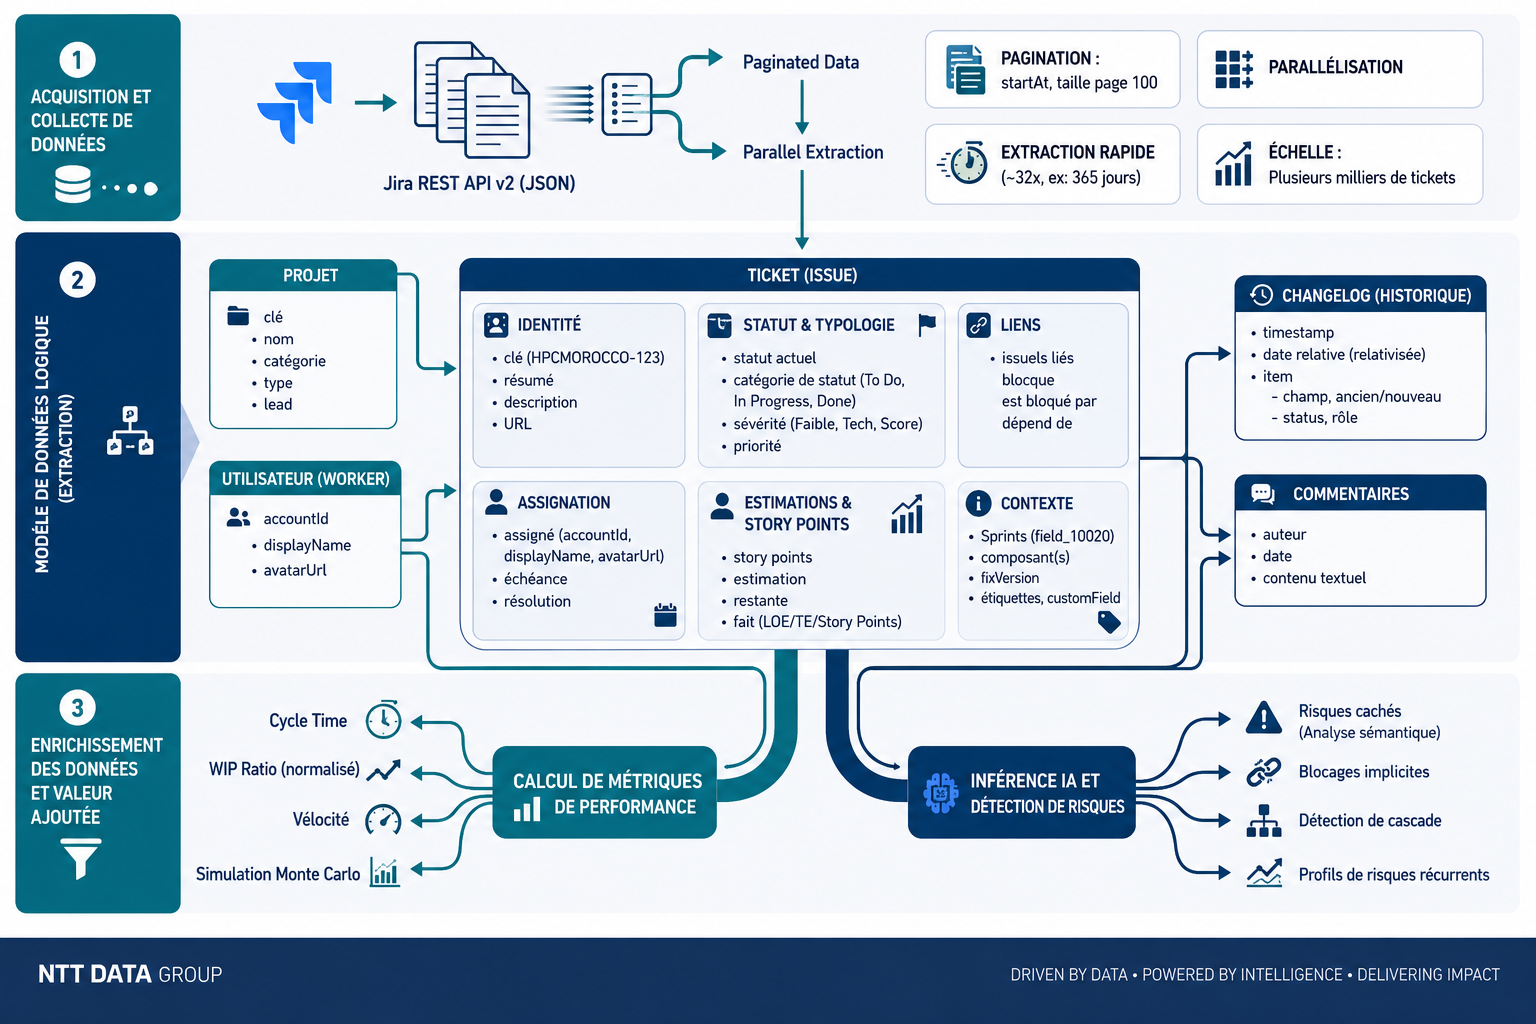
\includegraphics[width=0.9\linewidth]{assets/description_donnees.png}
\caption{Processus de traitement des données Jira et flux de métriques}
\label{fig:processus_donnees}
\end{figure}

Le processus global de traitement des données est illustré par la figure \ref{fig:processus_donnees}.

\subsection{Normalisation structurelle et aplatissement du changelog}
\label{subsec:normalisation}
Le JSON hétérogène retourné par l’API est passé dans des modèles Pydantic stricts (ex. \texttt{NormalizedIssueModel}) qui :
\begin{itemize}
    \renewcommand{\labelitemi}{—}
    \item Valident les types et la présence des champs obligatoires.
    \item Réorganisent l’information en quatre blocs : \texttt{identity}, \texttt{temporality}, \texttt{semantics}, \texttt{actors}.
    \item Convertissent les chaînes ISO en objets \texttt{datetime} (fuseau UTC) pour faciliter les calculs temporels.
    \item Aplatissent le \texttt{changelog} pour extraire la date de dernière transition et calculer le temps passé dans chaque statut (cycle time) – ce qui permet de déterminer \texttt{days\_since\_update} pour les tickets.
\end{itemize}
La normalisation élimine les variations inutiles (ex. champs \texttt{fields} imbriqués) et produit un objet Python homogène.

\subsection{Standardisation sémantique}
Les statuts Jira étant libres et personnalisables par chaque projet, nous appliquons une fonction de mappage (\texttt{jira\_canonical\_status}) qui traduit les noms bruts (ex. “En Cours”, “In Progress”, “Open”) vers quatre catégories canoniques :
\begin{itemize}
    \renewcommand{\labelitemi}{—}
    \item \texttt{todo} : tout statut initial ou ouvert non commencé.
    \item \texttt{in\_progress} : travail engagé.
    \item \texttt{done} : statuts de résolution (Fermé, Résolu, Livré).
    \item \texttt{unknown} : statut non reconnu (pour debug).
\end{itemize}
Cette standardisation permet de calculer le WIP ratio indépendamment des conventions de nommage.

\subsection{Agrégation pour le module Worker Insights}
\label{subsec:worker_aggregation}
Le module Worker Insights nécessite une préparation spécifique des données par développeur. La fonction \texttt{\_build\_worker\_snapshots()} regroupe les tickets par \texttt{assignee} et calcule pour chaque développeur les métriques suivantes : total de tickets assignés, tâches terminées, en cours, bloquées, taux de retard et temps de cycle moyen. Ces indicateurs sont complétés par les moyennes d’équipe (\texttt{avg\_completed}, \texttt{avg\_wip}, \texttt{avg\_assigned}) servant de référentiel de comparaison pour l’agent IA.

\subsection{Ingénierie des caractéristiques et préparation du contexte LLM}
Pour la simulation Monte Carlo, nous transformons l’historique des résolutions en un vecteur de comptages hebdomadaires (modèle « sac de billes ») afin d’optimiser les tirages aléatoires vectorisés via NumPy. Par ailleurs, pour l’agent IA, nous assemblons un prompt système structuré qui injecte les métriques calculées, les résultats du moteur de règles et les tickets actifs. La gestion de la fenêtre de contexte (limite de tokens) est assurée par la bibliothèque \texttt{tiktoken}, garantissant que la requête adressée à Mistral respecte les capacités du modèle.

\subsection{Stockage et mise en cache}
\label{subsec:stockage_cache}
Pour éviter des appels répétitifs à l’API et garantir la réactivité, une stratégie de cache multi‑niveaux est mise en œuvre :
\begin{itemize}
    \renewcommand{\labelitemi}{—}
    \item Les tickets normalisés sont stockés dans Redis avec une clé du type \texttt{project:HPCMOROCCO:issues} et un TTL de 15 minutes.
    \item Les résultats de la simulation Monte Carlo sont conservés pendant 24 heures (car l’historique varie peu à court terme).
    \item Les snapshots du module Worker Insights sont mis en cache avec un TTL de 15 minutes.
    \item En cas d’indisponibilité de Redis, le système bascule sur des fichiers JSON locaux (cache de secours) pour ne pas interrompre le service.
\end{itemize}

\section{Conclusion}
Ce chapitre a exposé l’intégralité du cycle de vie des données au sein de notre plateforme : extraction depuis l’API REST de Jira via des requêtes JQL optimisées, normalisation rigoureuse via des modèles Pydantic (incluant l’aplatissement du changelog), calcul de métriques de santé projet, simulation prédictive par Monte Carlo, agrégation pour le module Worker Insights, préparation du contexte pour le LLM, et visualisation dans un tableau de bord React ainsi que dans Grafana. La mise en cache intelligente (Redis) et les mécanismes de résilience garantissent des performances élevées tout en respectant les quotas de l’API. Ces données préparées et enrichies servent directement de combustible à l’agent IA conversationnel (LangGraph + Mistral) et aux algorithmes de détection de risques, dont l’implémentation est détaillée dans le chapitre suivant.
	\chapter{Description des données}
\vspace{-1.5em}
\chaptertoc
\vspace{-2.5em}
\vspace{-0.5em}
\section{Introduction}
\vspace{-1em}
L’industrie aéronautique génère de grandes quantités de données. Ce chapitre présente d’abord les sources et la structure des jeux de données utilisés, puis les résultats de l’analyse exploratoire (\ac{AED}) permettant d’identifier les tendances et anomalies. Il détaille ensuite les étapes de prétraitement nécessaires pour préparer les données à l’analyse.

\vspace{-1.5em}
\section{Source des données}
\vspace{-0.7em}
L’ensemble de données utilisé dans cette étude provient des processus opérationnels liés à la planification des vols saisonniers dans les aéroports marocains. Plus précisément, les données sont issues des horaires de vol soumis par les compagnies aériennes, validés par le \ac{MSC}, puis traités par \ac{CPV}. Ces informations sont initialement échangées sous forme de fichiers Excel, ajustées manuellement, puis intégrées dans le système \ac{SOAM} pour l’allocation des ressources aéroportuaires.  

\begin{figure}[H]
	\centering
	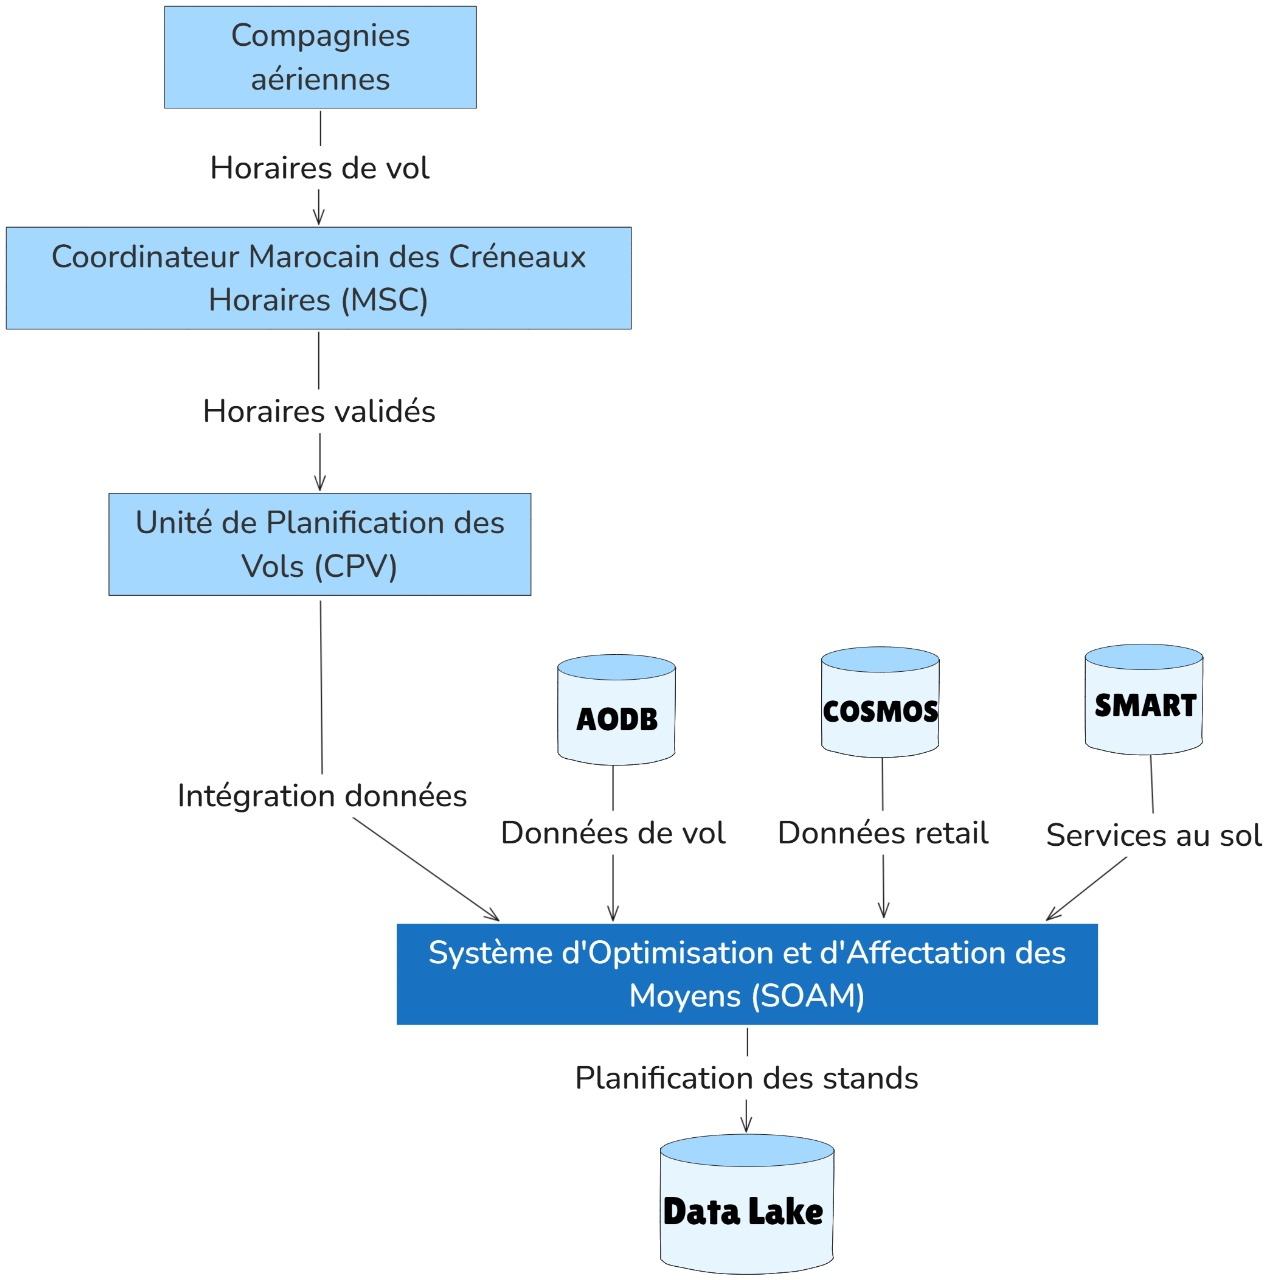
\includegraphics[width=0.6\linewidth]{assets/dataset/flux Données.jpg}
	\caption{Flux de données}
	\label{fig:flux_donnees}
\end{figure}


Le schéma \ref{fig:flux_donnees} illustre le flux de données depuis les compagnies aériennes jusqu'à l'intégration dans le \ac{SOAM}.
Les données exploitées dans cette étude couvrent un large spectre d’informations relatives à la planification des stands, comprenant des éléments statiques et dynamiques.

\subsection*{Synthèse des Sources de Données}
Les données exploitées proviennent de différentes sources internes et externes.

\noindent\textbf{Métadonnées des flux}~: Données extraites des tables Oracle, mises à jour toutes les 2h (quasi temps réel), avec un chargement initial complet puis des mises à jour incrémentales. Formats : JSON/Excel. Protocole à définir selon les systèmes.

\vspace{0.8em}
\noindent\textbf{Catégories de données opérationnelles} :
\begin{itemize}
	\item \textbf{Vols} (\acs{AODB})~: arrivées, départs, retards, statuts, mouvements, horaires ajustés, type de vol.
	\item \textbf{Avions et stands}~: types d’appareils, occupation des stands, durée escale, night stops, capacités, référentiels.
	\item \textbf{Infrastructure et sécurité}~: proximité équipements (passerelles, carburant), séparations de sécurité, zones sensibles, stands maintenance.
	\item \textbf{Données complémentaires}~: météo, consommation énergétique, activité commerciale (\textsc{COSMOS}/SMART).
\end{itemize}


\subsection*{Répartition de Source de données}
La répartition des sources de données, illustrée dans la Figure \ref{fig:enter-label}, montre une prédominance marquée de l'\ac{AODB}, qui représente à elle seule 70 \% des sources utilisées. Les aéroports contribuent pour 15 \%, tandis que les autres sources, notamment COSMOS/SMART, se partagent les 15 \% restants. Cette distribution met en évidence la centralité de l'\ac{AODB} dans le système.
\begin{figure}[H]
	\centering
	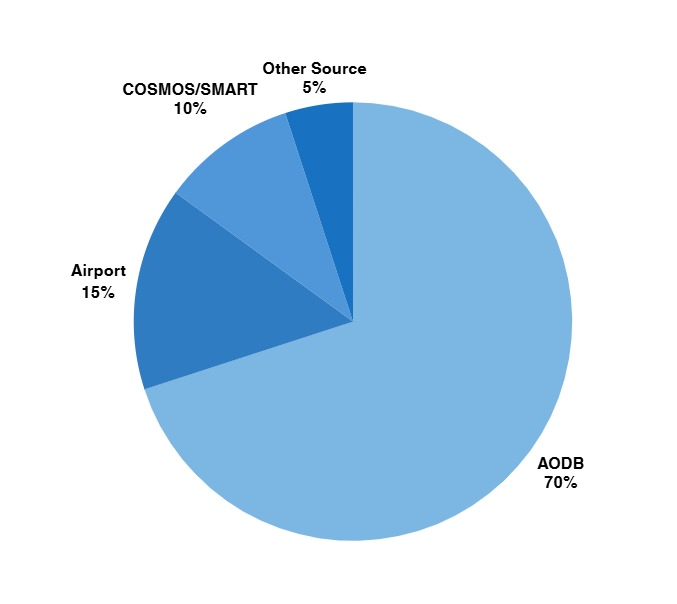
\includegraphics[width=0.5\linewidth]{assets/dataset/Distribution.jpg}
	\caption{Répartition de Catégories de données}
	\label{fig:enter-label}
\end{figure}

Toutes ces sources de données ont été exploitées dans le but de constituer un jeu de données unifié. Après l'étape de collecte, l’ensemble des informations a été consolidé en deux fichiers CSV finaux, utilisés comme base pour nos analyses.



\section{Description des données}
Dans cette étape, nous commençons par explorer la structure et le contenu de l'ensemble de données aéroportuaires pour comprendre ses composantes clés et les relations entre elles. Alors notre étude s'appuie sur deux jeux de données principaux :  

\_{Un dataset dédié aux départs de vols \textbf{(4945 observations, 485 variables)}}.  

\_{Un second relatif aux arrivées de vols \textbf{(5018 observations, 417 variables)}, partageant une structure similaire mais présentant des variations contextuelles dans l'agencement des lignes et de certaines colonnes.}

En raison de la complexité inhérente à ces données multidimensionnelles, une catégorisation thématique a été mise en place pour en faciliter l'analyse et l'interprétation. Cette segmentation, représentée par un organigramme dans la Figure~\ref{fig:dataset} qui regroupe les variables en catégories fonctionnelles:

\begin{itemize}
	\item \textbf{Vols et compagnies aériennes} : Cette catégorie regroupe les informations liées aux vols, aux compagnies aériennes, aux villes, aux avions, ainsi qu’aux aéroports concernés.
	\item \textbf{Infrastructures aéroportuaires} : Elle inclut des détails sur les terminaux, les stands, les portes d’embarquement et autres éléments liés aux installations de l’aéroport.
	\item \textbf{Temps et dates} : Cette catégorie regroupe les informations temporelles comme les horaires de départ et d’arrivée, planifiés et réels, les fuseaux horaires et les périodes d’exploitation.
	\item \textbf{Bagages et passagers} : Ce volet couvre les systèmes de gestion des bagages, les délais de traitement et les infrastructures associées.
	\item \textbf{Retards et irrégularités} : Contient des informations sur la durée des retards ainsi que les perturbations impactant les vols.
	\item \textbf{Opérations au sol} : Données sur les procédures avant départ ou après arrivée.
	\item \textbf{Divers} : Regroupe les variables hors des catégories précédentes.
\end{itemize}
\begin{figure}[H]
	\centering
	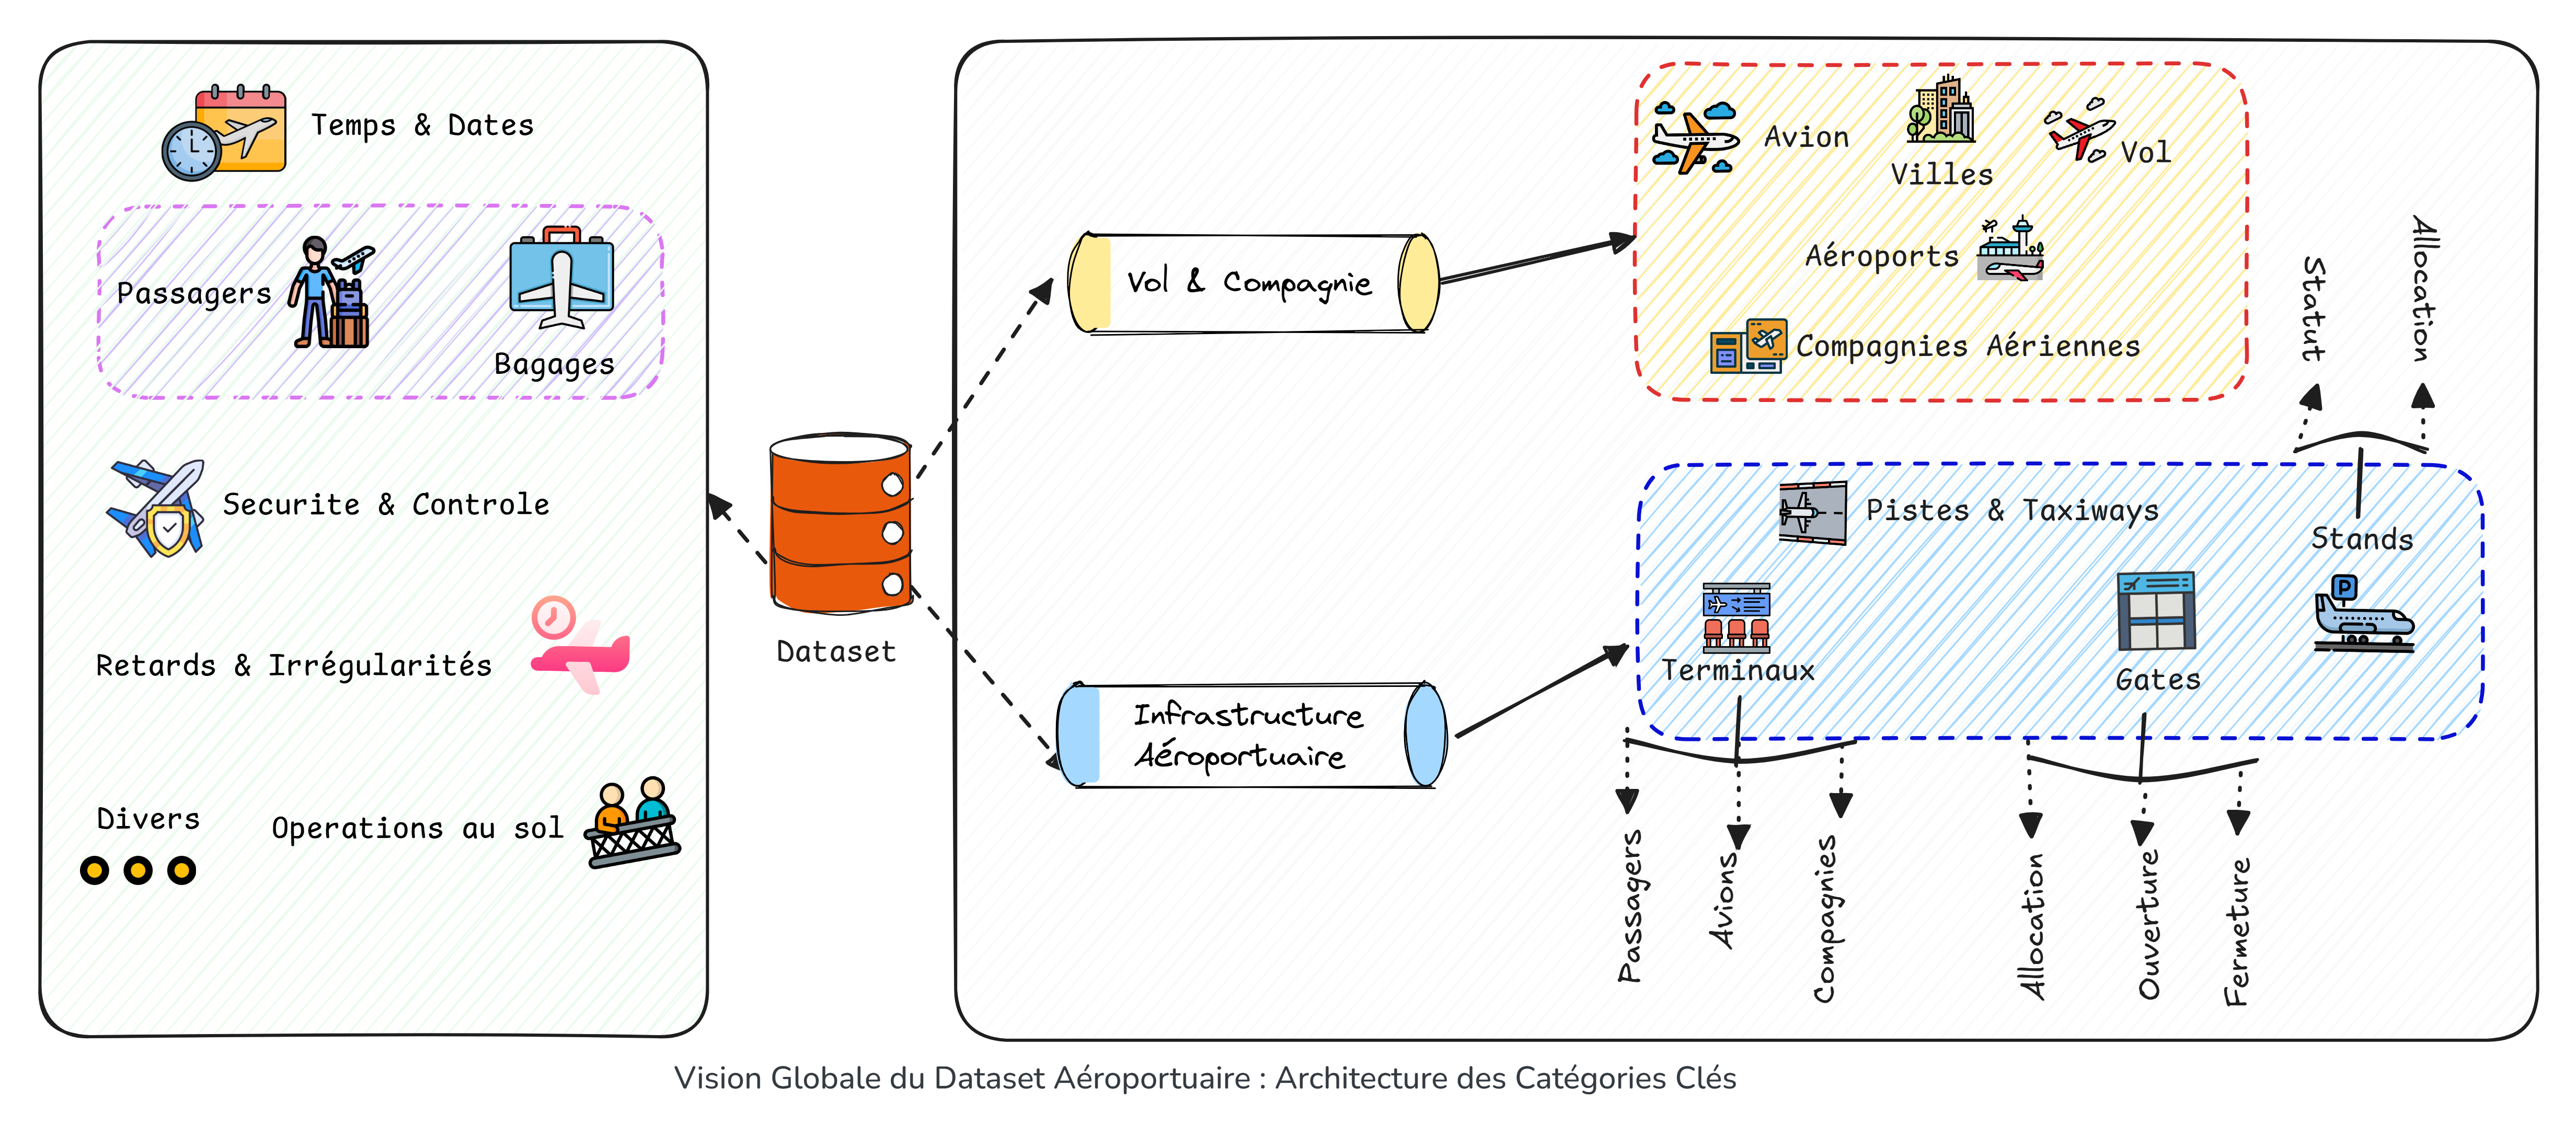
\includegraphics[width=0.9\linewidth]{assets/dataset/dataset.png}
	\caption{Illustration du dataset}
	\label{fig:dataset}
\end{figure}

Cette organisation favorise une analyse plus efficace du dataset en regroupant les informations selon leur nature et leur impact sur les opérations aéroportuaires. Elle facilite également l'interprétation des résultats et met en lumière les relations entre les différentes variables du dataset.

\subsection*{Vue d’ensemble des données opérationnelles}
Le tableau \ref{tab:synthese_operationnelle} ci-dessous résume les principales caractéristiques du jeu de données utilisé dans cette étude. Il s'agit de données opérationnelles collectées sur une période de deux mois (novembre et décembre 2024).

\begin{table}[H]
	\centering
	\renewcommand{\arraystretch}{0.9} % réduit l'espacement vertical
	\caption{Synthèse des données opérationnelles aéroportuaires}
	\begin{tabularx}{\textwidth}{@{}>{\bfseries}l X@{}}
		\toprule
		\textbf{Paramètre} & \textbf{Caractéristiques} \\
		\midrule
		Période du trafic          & 2 mois (Novembre \& Décembre 2024) \\
		Volume de trafic           & 9\,963 vols \\
		Variables – Dataset départ & 485 \\
		Variables – Dataset arrivée& 417 \\
		Opérateurs aériens         & 46 compagnies aériennes \\
		Catégorie opérationnelle   & Transport de passagers \\
		Nombre de stands           & 65 stands de stationnement \\
		Type de vols               & International / Domestique \\
		Vols Schengen              & SCH ou non \\
		Type d'avion               & A320, B737, B787, A330, A380 \\
		Classification des retards & Aucun, Faible, Moyen, Élevé, Majeur \\
		\bottomrule
	\end{tabularx}

	\label{tab:synthese_operationnelle}
\end{table}

\noindent
Il est important de noter que les données disponibles couvrent uniquement une période de deux mois. En réalité, l'aéroport traite un volume bien plus important : un plus grand nombre de compagnies aériennes, une diversité accrue de types d’avions, ainsi que 83 stands utilisés, incluant ceux destinés aux vols réguliers, au fret (cargo) et à la maintenance (hangars).




\section{Analyse et Visualisation des Données}

Pour acquérir une compréhension approfondie de l'ensemble de données aéroportuaires et en tirer des insights significatifs, un cadre d’analyse structuré a été établi. Celui-ci commence par le prétraitement des données brutes — incluant les vols, les stands, les portes d'embarquement, les terminaux et les retards — à travers des étapes de nettoyage et de transformation.

L’ensemble de données est ensuite exploré selon trois axes analytiques principaux :
\begin{itemize}
	\item \textbf{Analyse des vols} : étude des caractéristiques des vols, des horaires, des types d’appareils, ainsi que des compagnies aériennes les plus actives.
	\item \textbf{Analyse des stands} : évaluation du nombre total de stands, des compagnies utilisatrices, et de la durée moyenne de stationnement.
	\item \textbf{Analyse des retards} : analyse des vols retardés, des durées maximales de retard et des compagnies les plus fréquemment concernées.
\end{itemize}

Les résultats obtenus permettent d’identifier des modèles clés tels que les taux d’occupation, les flux horaires et les tendances de trafic. Cette compréhension globale facilite la production de visualisations claires et éclairées la planification optimale des ressources aéroportuaires.

\subsection{Analyse des vols}

Dans cette partie, une analyse des caractéristiques générales des vols du dataset a été réalisée, visant à identifier les tendances liées aux horaires, aux compagnies aériennes et aux types d’avions.

\begin{figure}[H]
	\centering
	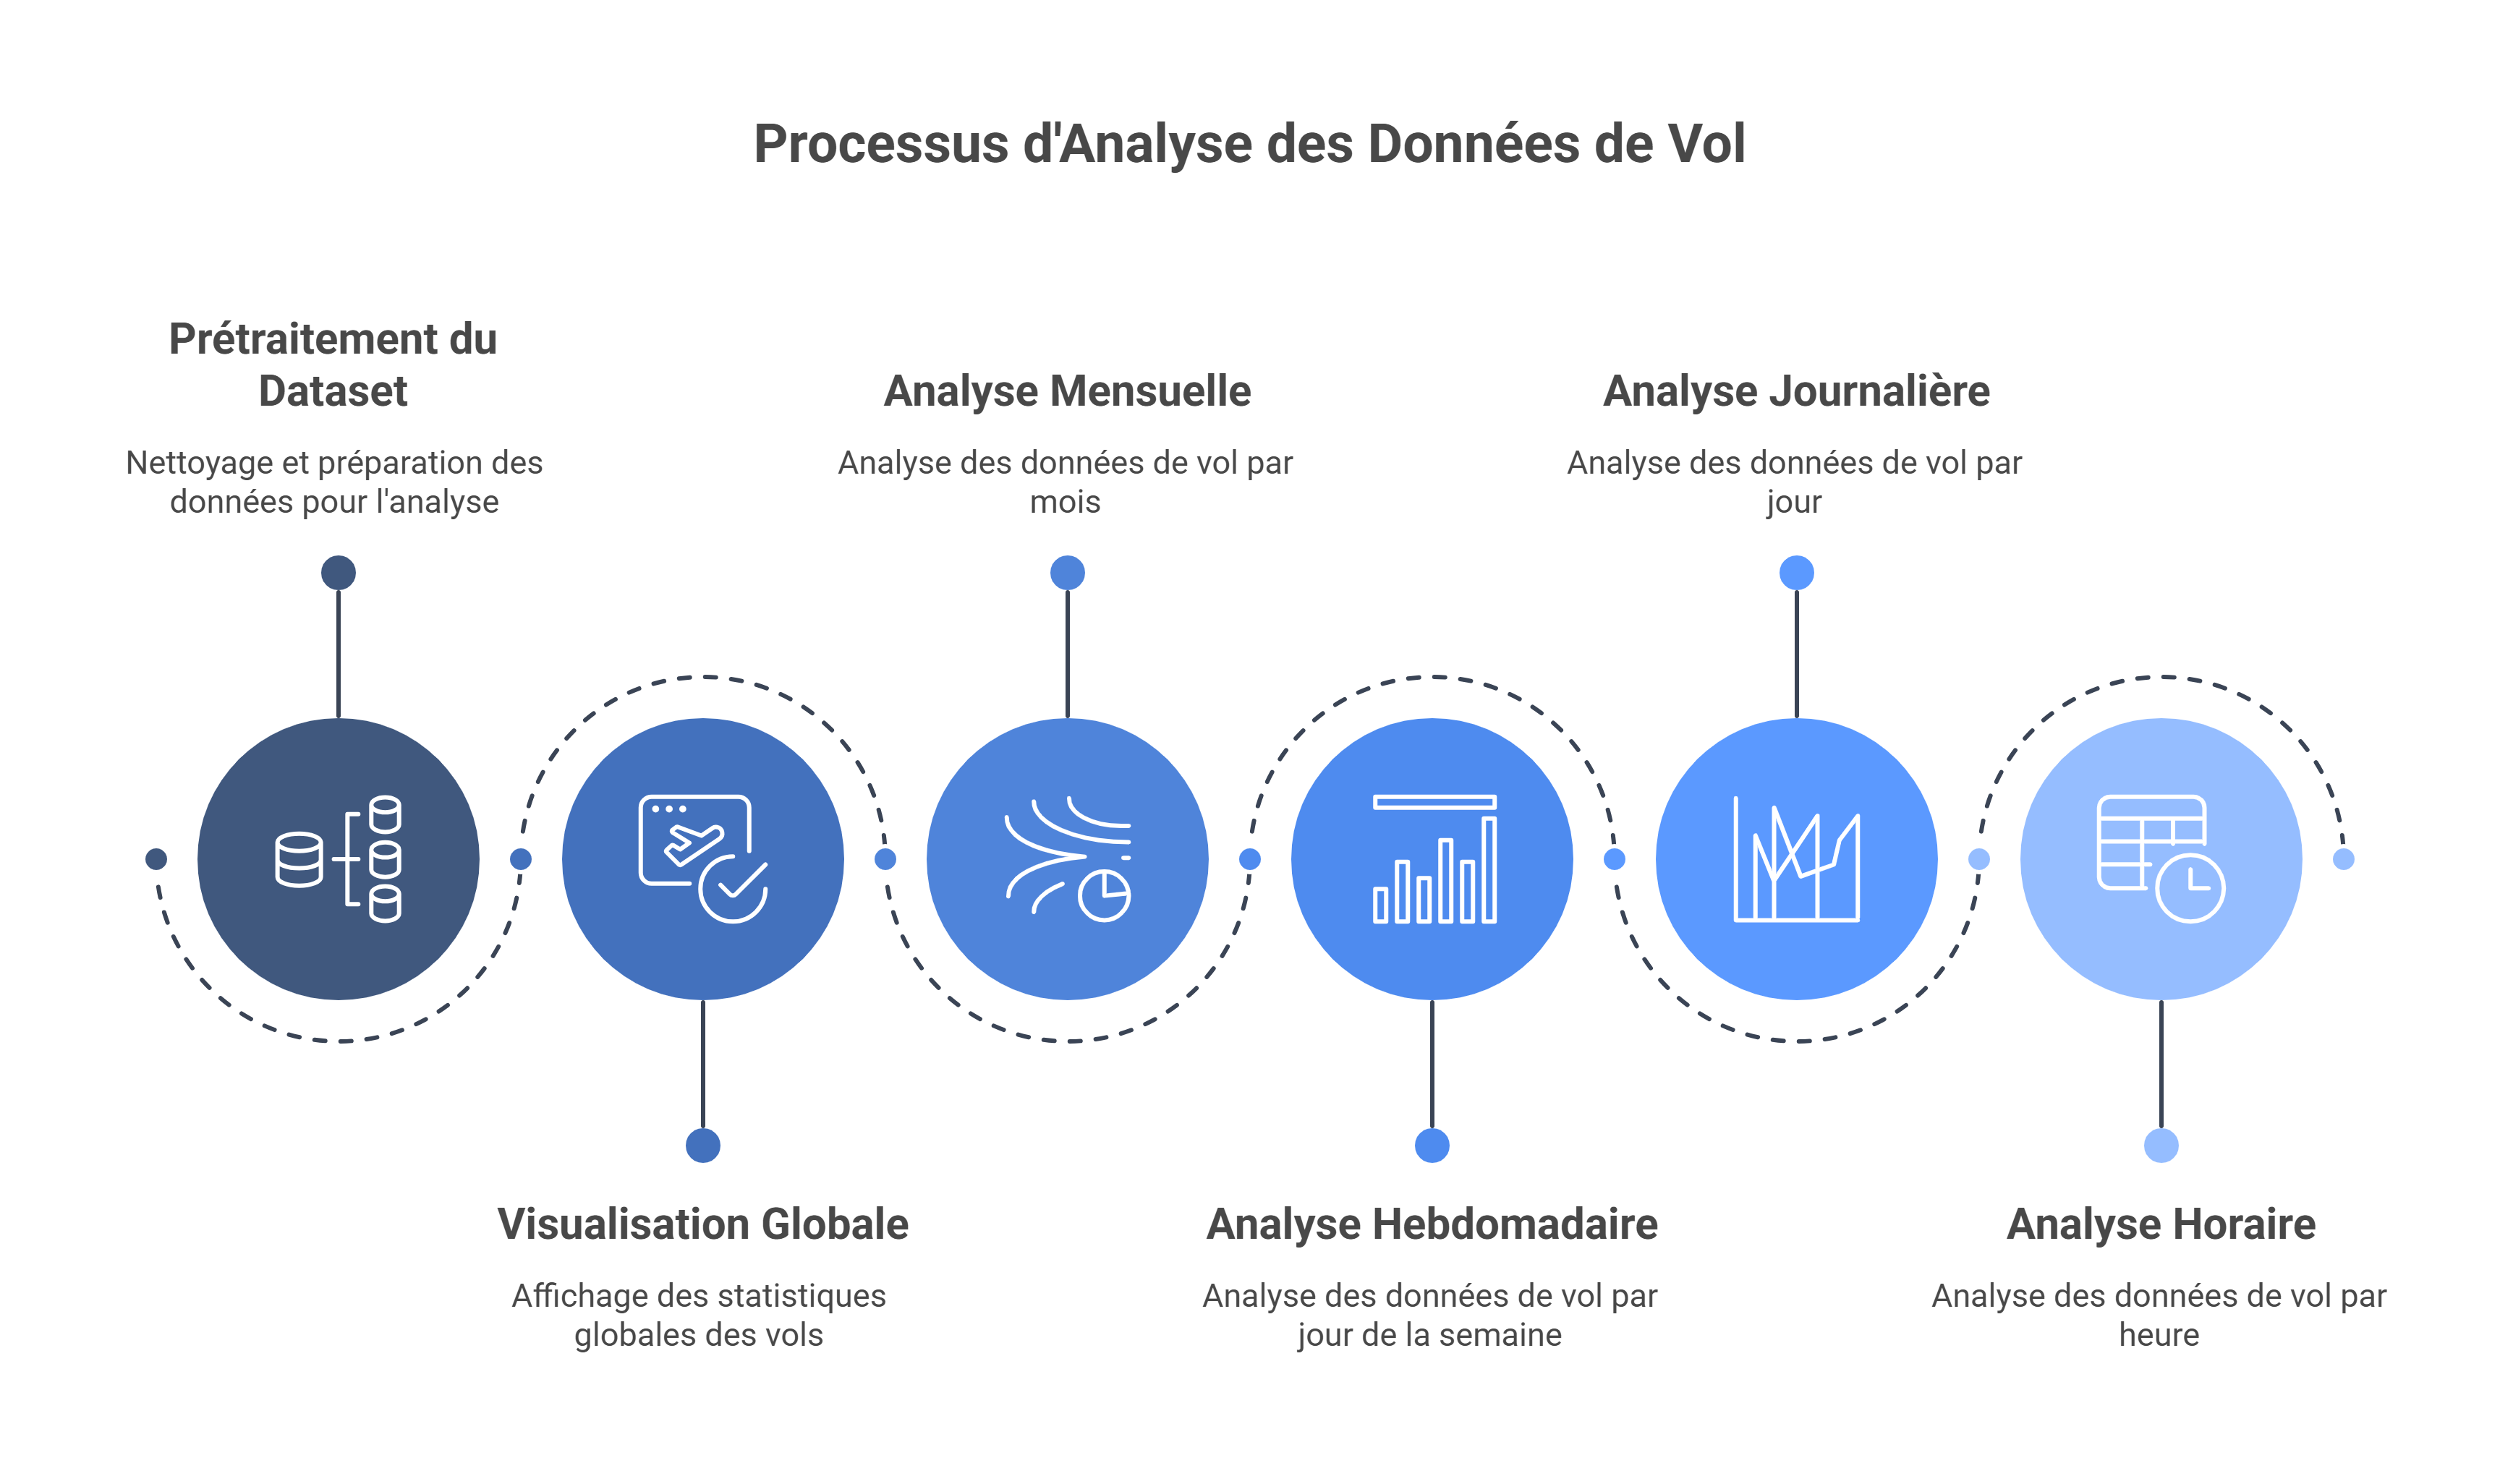
\includegraphics[width=0.8\textwidth]{assets/dataset/vol1.png}
	\caption{Flux du processus d'analyse des vols.}
	\label{fig:flight_analysis_flow}
\end{figure}

Afin d’assurer un processus méthodique, l’analyse suit la structure décrite ci-dessous :

Tout d’abord, une phase de prétraitement est effectuée pour préparer les données à l’analyse.  
Ensuite, une visualisation globale est réalisée afin d’avoir une vue d’ensemble du jeu de données.  
L’analyse est ensuite affinée selon trois niveaux temporels: \begin{itemize}
	\item Une analyse mensuelle pour identifier les tendances générales,
	\item Une analyse hebdomadaire pour un suivi plus précis,
	\item Une analyse journalière pour détecter les variations quotidiennes.
\end{itemize}

Enfin, une analyse horaire est menée afin de mieux comprendre la dynamique des vols selon les différentes tranches horaires de la journée.

Cette approche progressive permet d’avoir une vision détaillée du comportement des vols.  
\subsubsection{prétraitement de données}
Avant de procéder à l’analyse principale, une phase de prétraitement essentielle
est réalisée afin de préparer le jeu de données. Cette étape garantit que les données
sont propres, pertinentes et correctement structurées pour les opérations à venir. Le
prétraitement suit le schéma illustré ci-dessous.
\begin{figure}[H]
	\centering
	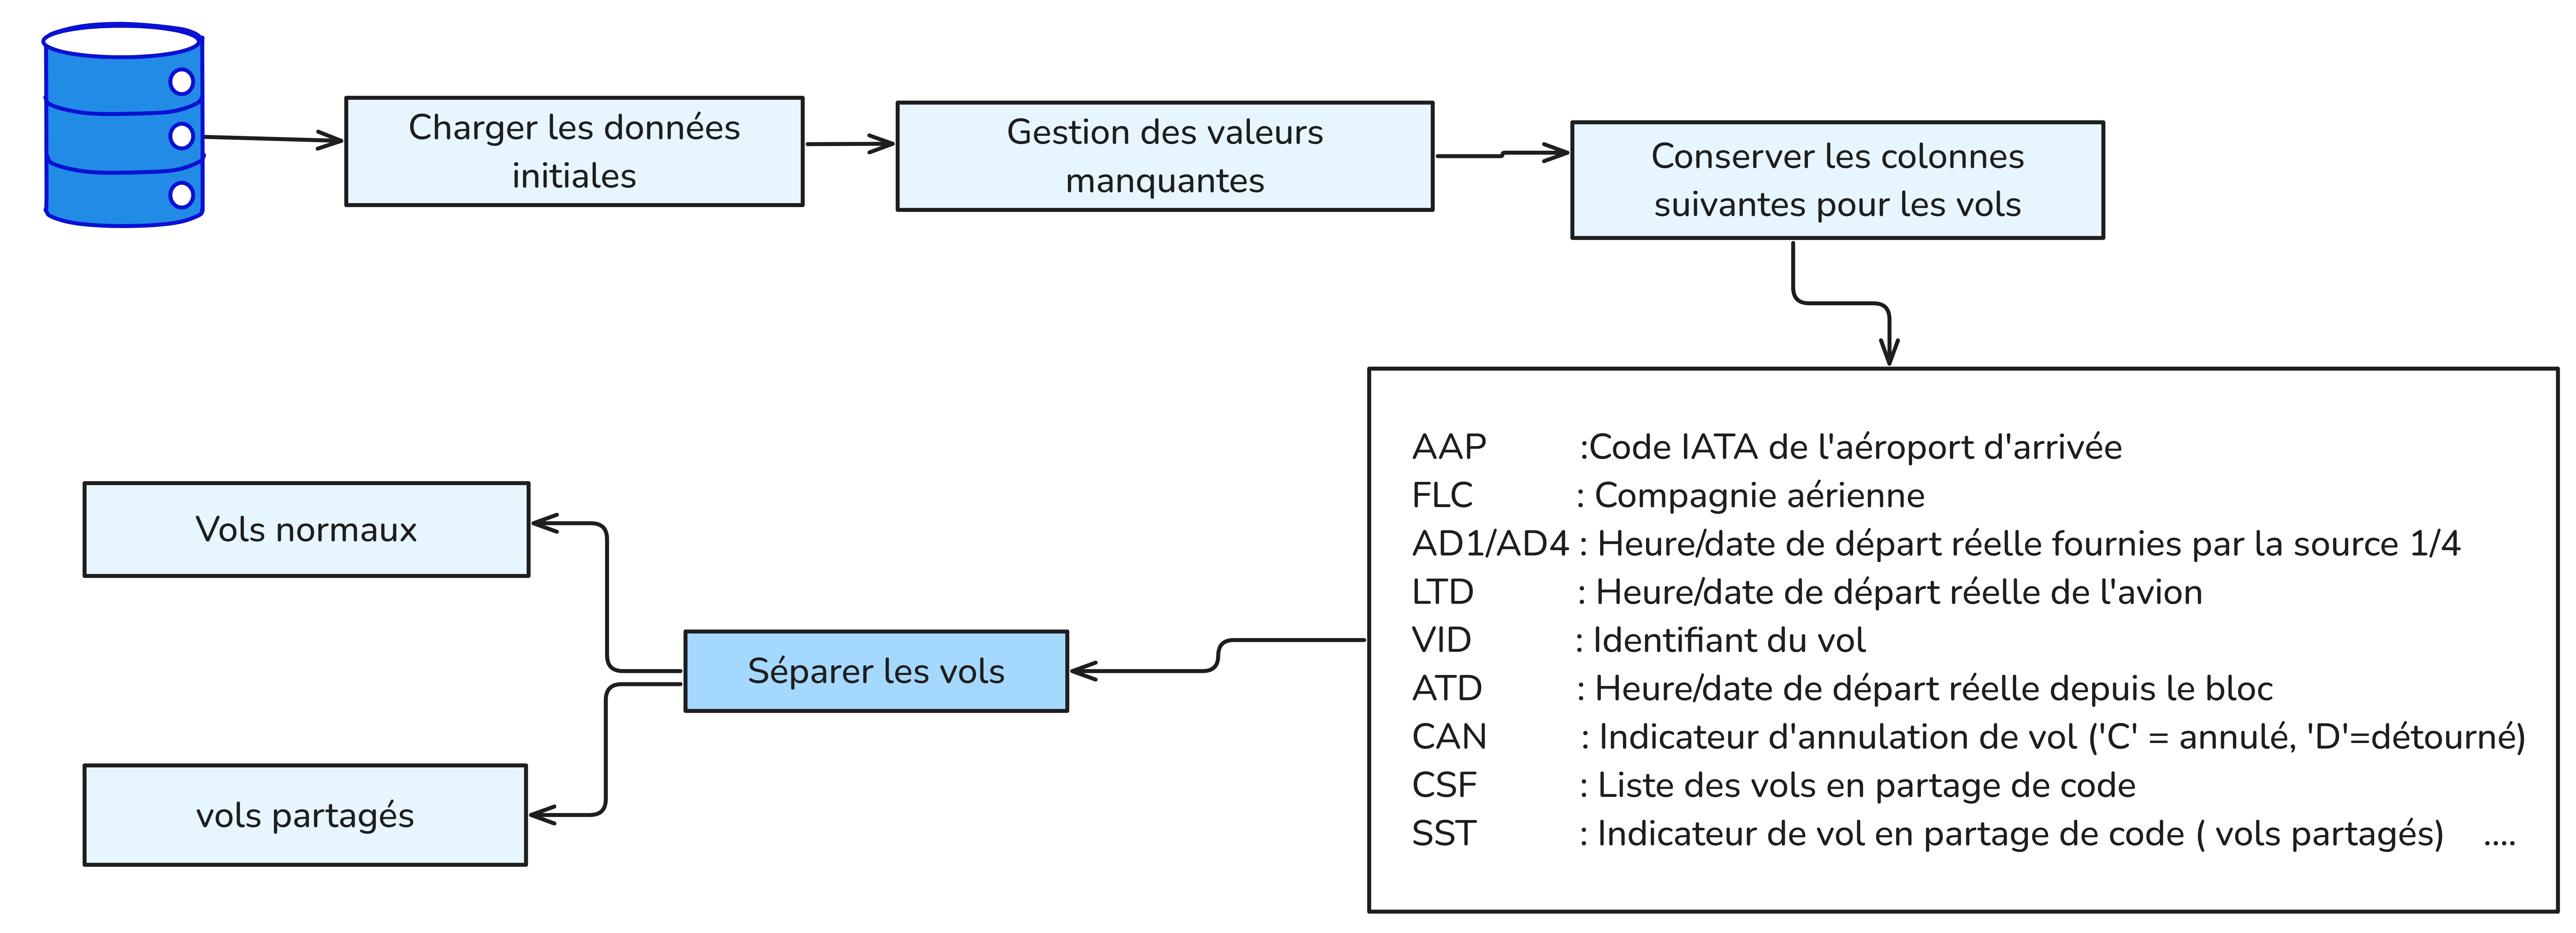
\includegraphics[width=0.9\textwidth]{assets/dataset/preprocessing.png} % adapt the filename
	\caption{Organigramme du prétraitement du jeu de données.}
	\label{fig:preprocessing_flowchart}
\end{figure}

Le prétraitement comprend les étapes suivantes :

\begin{itemize}
	\item\textbf{Chargement du jeu de données initial}:
	Le jeu de données original contenant les informations sur les vols est importé dans le système.
	
	\item \textbf{Traitement des valeurs manquantes} : Les entrées manquantes ou incomplètes sont gérées afin d’assurer la cohérence du jeu de données, notamment à l’aide de techniques d’imputation (comme la substitution par la moyenne, la médiane ou des valeurs prédites).
	
	
	\item \textbf{ Sélection des colonnes pertinentes}: Seules les colonnes essentielles à l’analyse des vols sont conservées. Celles-ci incluent les identifiants des vols, les heures de départ et d’arrivée, les compagnies aériennes, les indicateurs d’annulation, et les marqueurs de vols partagés.
	
	\item \textbf{Séparation des vols}: Le jeu de données est divisé en deux catégories :
	\begin{itemize}
		\item \textit{Vols normaux}: Vols standards, indépendants.
		\item \textit{Vols en partage de code}: Vols opérés dans le cadre d’un accord de partage de code entre plusieurs compagnies.
	\end{itemize}
\end{itemize}

Ce prétraitement permet d’assurer que les données utilisées pour l’analyse sont
à la fois propres et spécifiquement adaptées aux objectifs de l’étude. 

\subsubsection{Analyse Globale du Jeu de Données}

Pour initier notre étude, une analyse globale du jeu de données a été réalisée à travers diverses visualisations afin de mieux comprendre la structure sous-jacente des données.

Dans un premier temps, nous avons examiné la tendance globale du trafic aérien sur la période de deux mois étudiée. Nous avons observé un pic d’activité en novembre, indiquant une augmentation significative du nombre de vols par rapport au mois suivant.

Ensuite, nous avons analysé la répartition des vols par compagnie aérienne. Cette analyse a révélé que la compagnie \textbf{\ac{AT}} a opéré le plus grand nombre de vols, suivie par \textbf{3O} (Air Arabia) et \textbf{AF} (Air France).
\begin{figure}[H]
	\centering
	\begin{minipage}{0.25\textwidth}
		\centering
		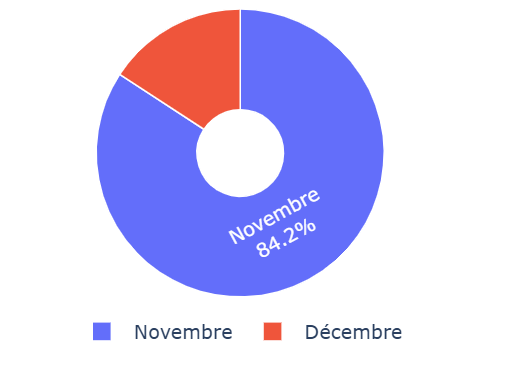
\includegraphics[width=\linewidth]{assets/dataset/repartitionpourcen.png}
		\small a) La tendance des vols globale entre novembre et décembre
	\end{minipage}
	\hfill
	\begin{minipage}{0.7\textwidth}
		\centering
		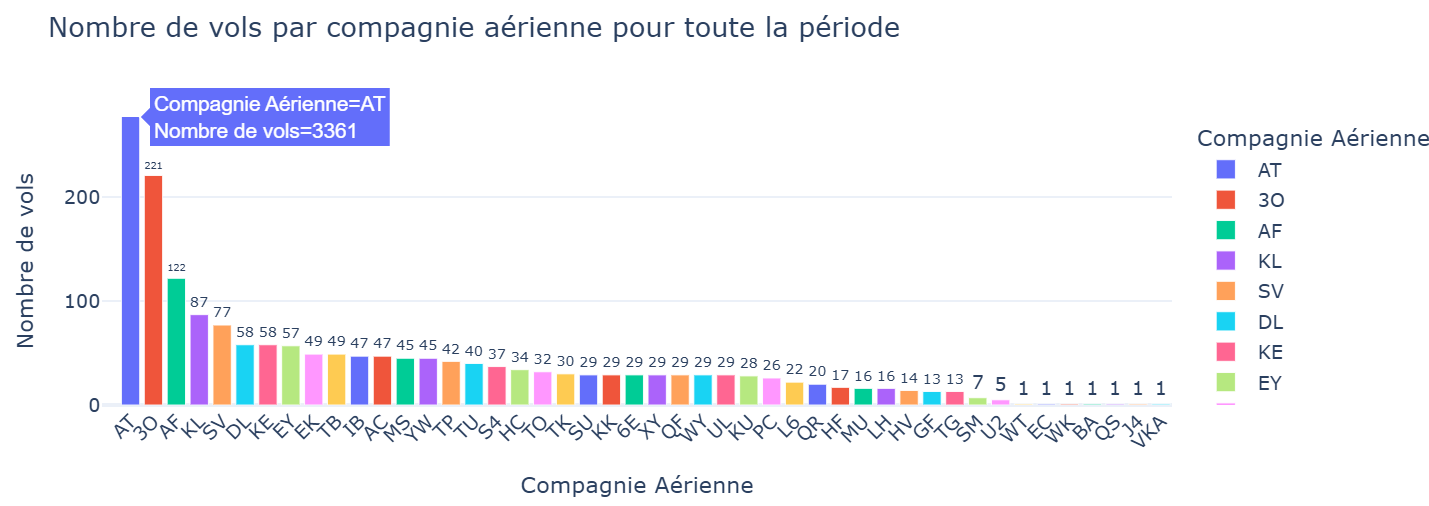
\includegraphics[width=\linewidth]{assets/dataset/nmbrvols.png}
		\small b) Répartition des vols par compagnie aérienne
	\end{minipage}
	
	\captionsetup{justification=centering}
	\caption{Les Vols en (novembre -décembre.) et répartition par compagnie.}
	\label{fig:analyse_trafic}
\end{figure}
\vspace{-0.5cm}
Le jeu de données distinguant deux types de vols: les \textbf{\textit{vols normaux}} et les \textbf{\textit{vols en partage de code}}. Nous avons approfondi l’analyse de leur répartition. Un vol en partage de code est défini comme un vol opéré par une compagnie aérienne mais commercialisé sous plusieurs numéros de vols par des compagnies partenaires,
éventuellement associées à différents codes des compagnies aériennes.
\newline
Notre analyse a montré que certaines compagnies n’opéraient que des vols en partage de code, sans présence opérationnelle directe. Par conséquent, ces compagnies ont été exclues du processus d’allocation des postes de stationnement. À l’inverse, l’attention a été portée sur les compagnies opérant leurs propres vols, qu’ils soient normaux ou en partage de code.  

La \textbf{Figure~\ref{fig:analyse_trafic}}  ainsi que La \textbf{Figure~\ref{fig:analyse_vols_partage}} 
ci-dessous illustre cette distinction.

\begin{figure}[H]
	\centering
	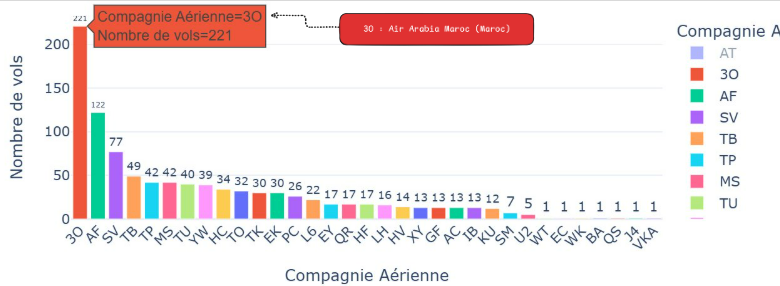
\includegraphics[width=0.95\textwidth]{assets/dataset/sansSF.png}
	\captionsetup{justification=centering}
	\caption{Vols par compagnie actives uniquement}
	\label{fig:analyse_vols_partage}
\end{figure}
 On y observe notamment que la compagnie \textbf{KL} (KLM Royal Dutch Airlines) est uniquement présente dans les vols en partage de code, ce qui indique qu’elle n'opère aucun vol avec ses propres aéronefs durant la période analysée.  
 
La \textbf{Figure~\ref{fig:vols_partages_compagnie}}  montre la répartition des vols partagés par compagnie .
\begin{figure}[H]
	\centering
	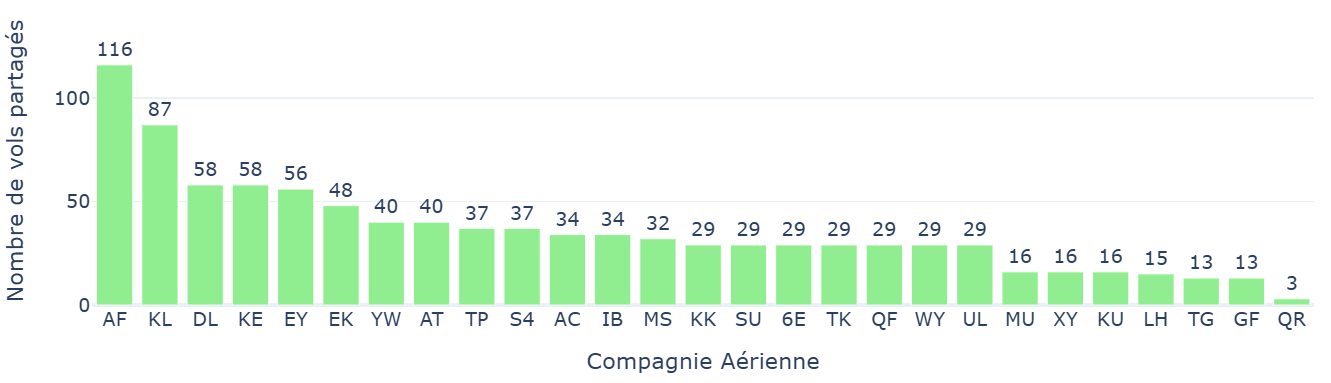
\includegraphics[width=1\textwidth]{assets/dataset/nbrvolsSF.png}
	\captionsetup{justification=centering}
	\caption{Vols partagés par compagnie}
	\label{fig:vols_partages_compagnie}
\end{figure}




Enfin, une attention particulière a été accordée aux taux d’annulation par compagnie aérienne. L’analyse de la proportion de vols annulés nous a permis de mieux comprendre la fiabilité de chaque compagnie et d’anticiper d’éventuelles perturbations dans les analyses ultérieures.

\subsubsection{Analyse Mensuelle, Hebdomadaire, Journalière et Horaire}

À la suite de l’analyse globale, nous avons procédé à une étude temporelle plus détaillée, en commençant par une décomposition mensuelle.

Étant donné que le mois de novembre a présenté le volume de vols le plus élevé, nous avons centré notre analyse sur ce mois. Nous avons ensuite ciblé les deux semaines présentant le pic d’activité au cours de novembre, afin d’obtenir une compréhension plus précise de la répartition du trafic.

La figure \ref{fig:repartition_vols_par_semaine} présente la répartition des vols par semaine pour le mois de Novembre
\begin{figure}[H]
	\centering
	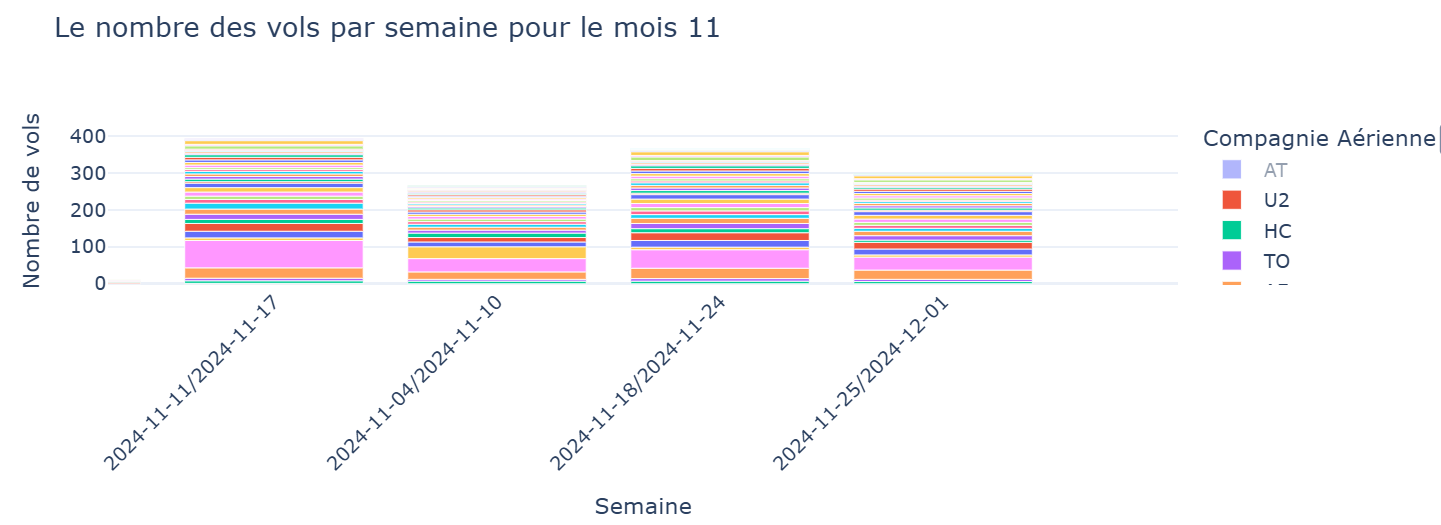
\includegraphics[width=1\textwidth]{assets/dataset/repartitionvolsparsemaine.png}
	\captionsetup{justification=centering}
	\caption{Répartition des vols par semaine}
	\label{fig:repartition_vols_par_semaine}
\end{figure}
Par la suite, nous avons affiné l’analyse en étudiant les tendances journalières et horaires. Cette approche de zoom progressif nous a permis d’identifier les jours les plus chargés ainsi que les heures de pointe, fournissant ainsi des informations critiques pour l’optimisation des opérations et l’allocation des postes de stationnement.
\begin{figure}[H]
	\centering
	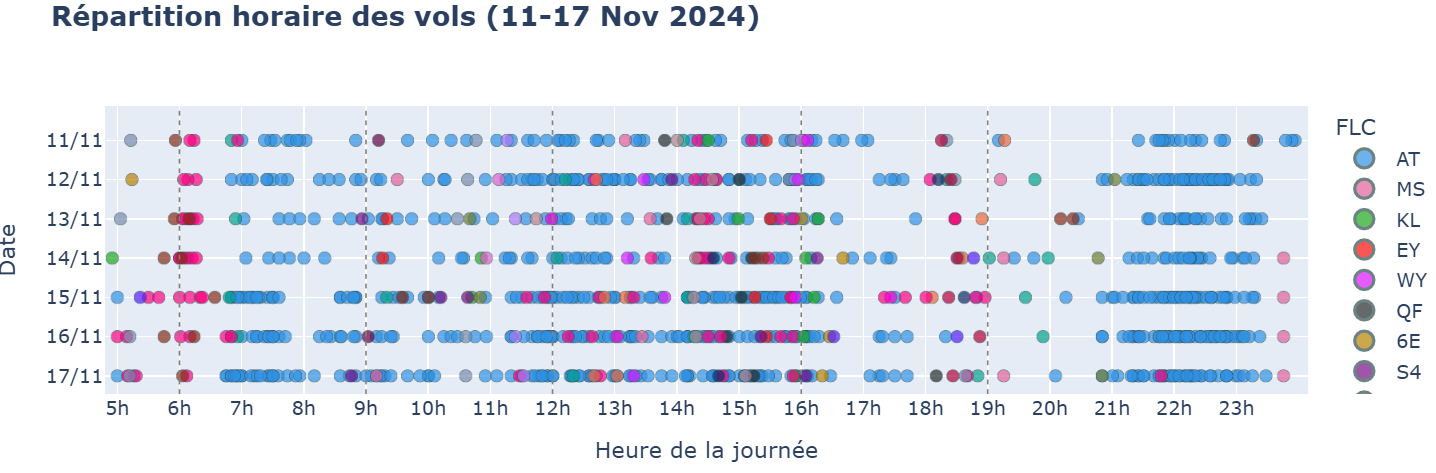
\includegraphics[width=1\textwidth]{assets/dataset/repartitionparheure.png}
	\captionsetup{justification=centering}
	\caption{Répartition des vols par heure durant la semaine la plus chargée}
	\label{fig:repartition_vols_par_heure}
\end{figure}
\vspace{-0.7em}
La figure montre une concentration du trafic entre \textbf{12h et 16h}, période durant laquelle le volume de vols atteint son pic.

\vspace{-0.7em}
\subsection{Analyse des stands}
De même, une analyse des caractéristiques générales des stands du dataset a été réalisée.
\subsubsection{Sélection des caractéristiques}

La première étape de l’analyse des stands a consisté en une sélection rigoureuse des caractéristiques pertinentes, comme illustré dans la figure~\ref{fig:stand-selection}. Plus précisément, nous avons retenu les colonnes directement liées à l’occupation des stands, à leur disponibilité, ainsi qu’à leur attribution au cours des périodes temporelles. Par la suite, une phase de prétraitement a été réalisée afin de traiter les valeurs manquantes, de standardiser les formats et d’assurer la cohérence des données. Ce travail préparatoire était essentiel pour permettre une analyse précise et fiable dans les étapes suivantes.


\begin{figure}[h]
	\centering
	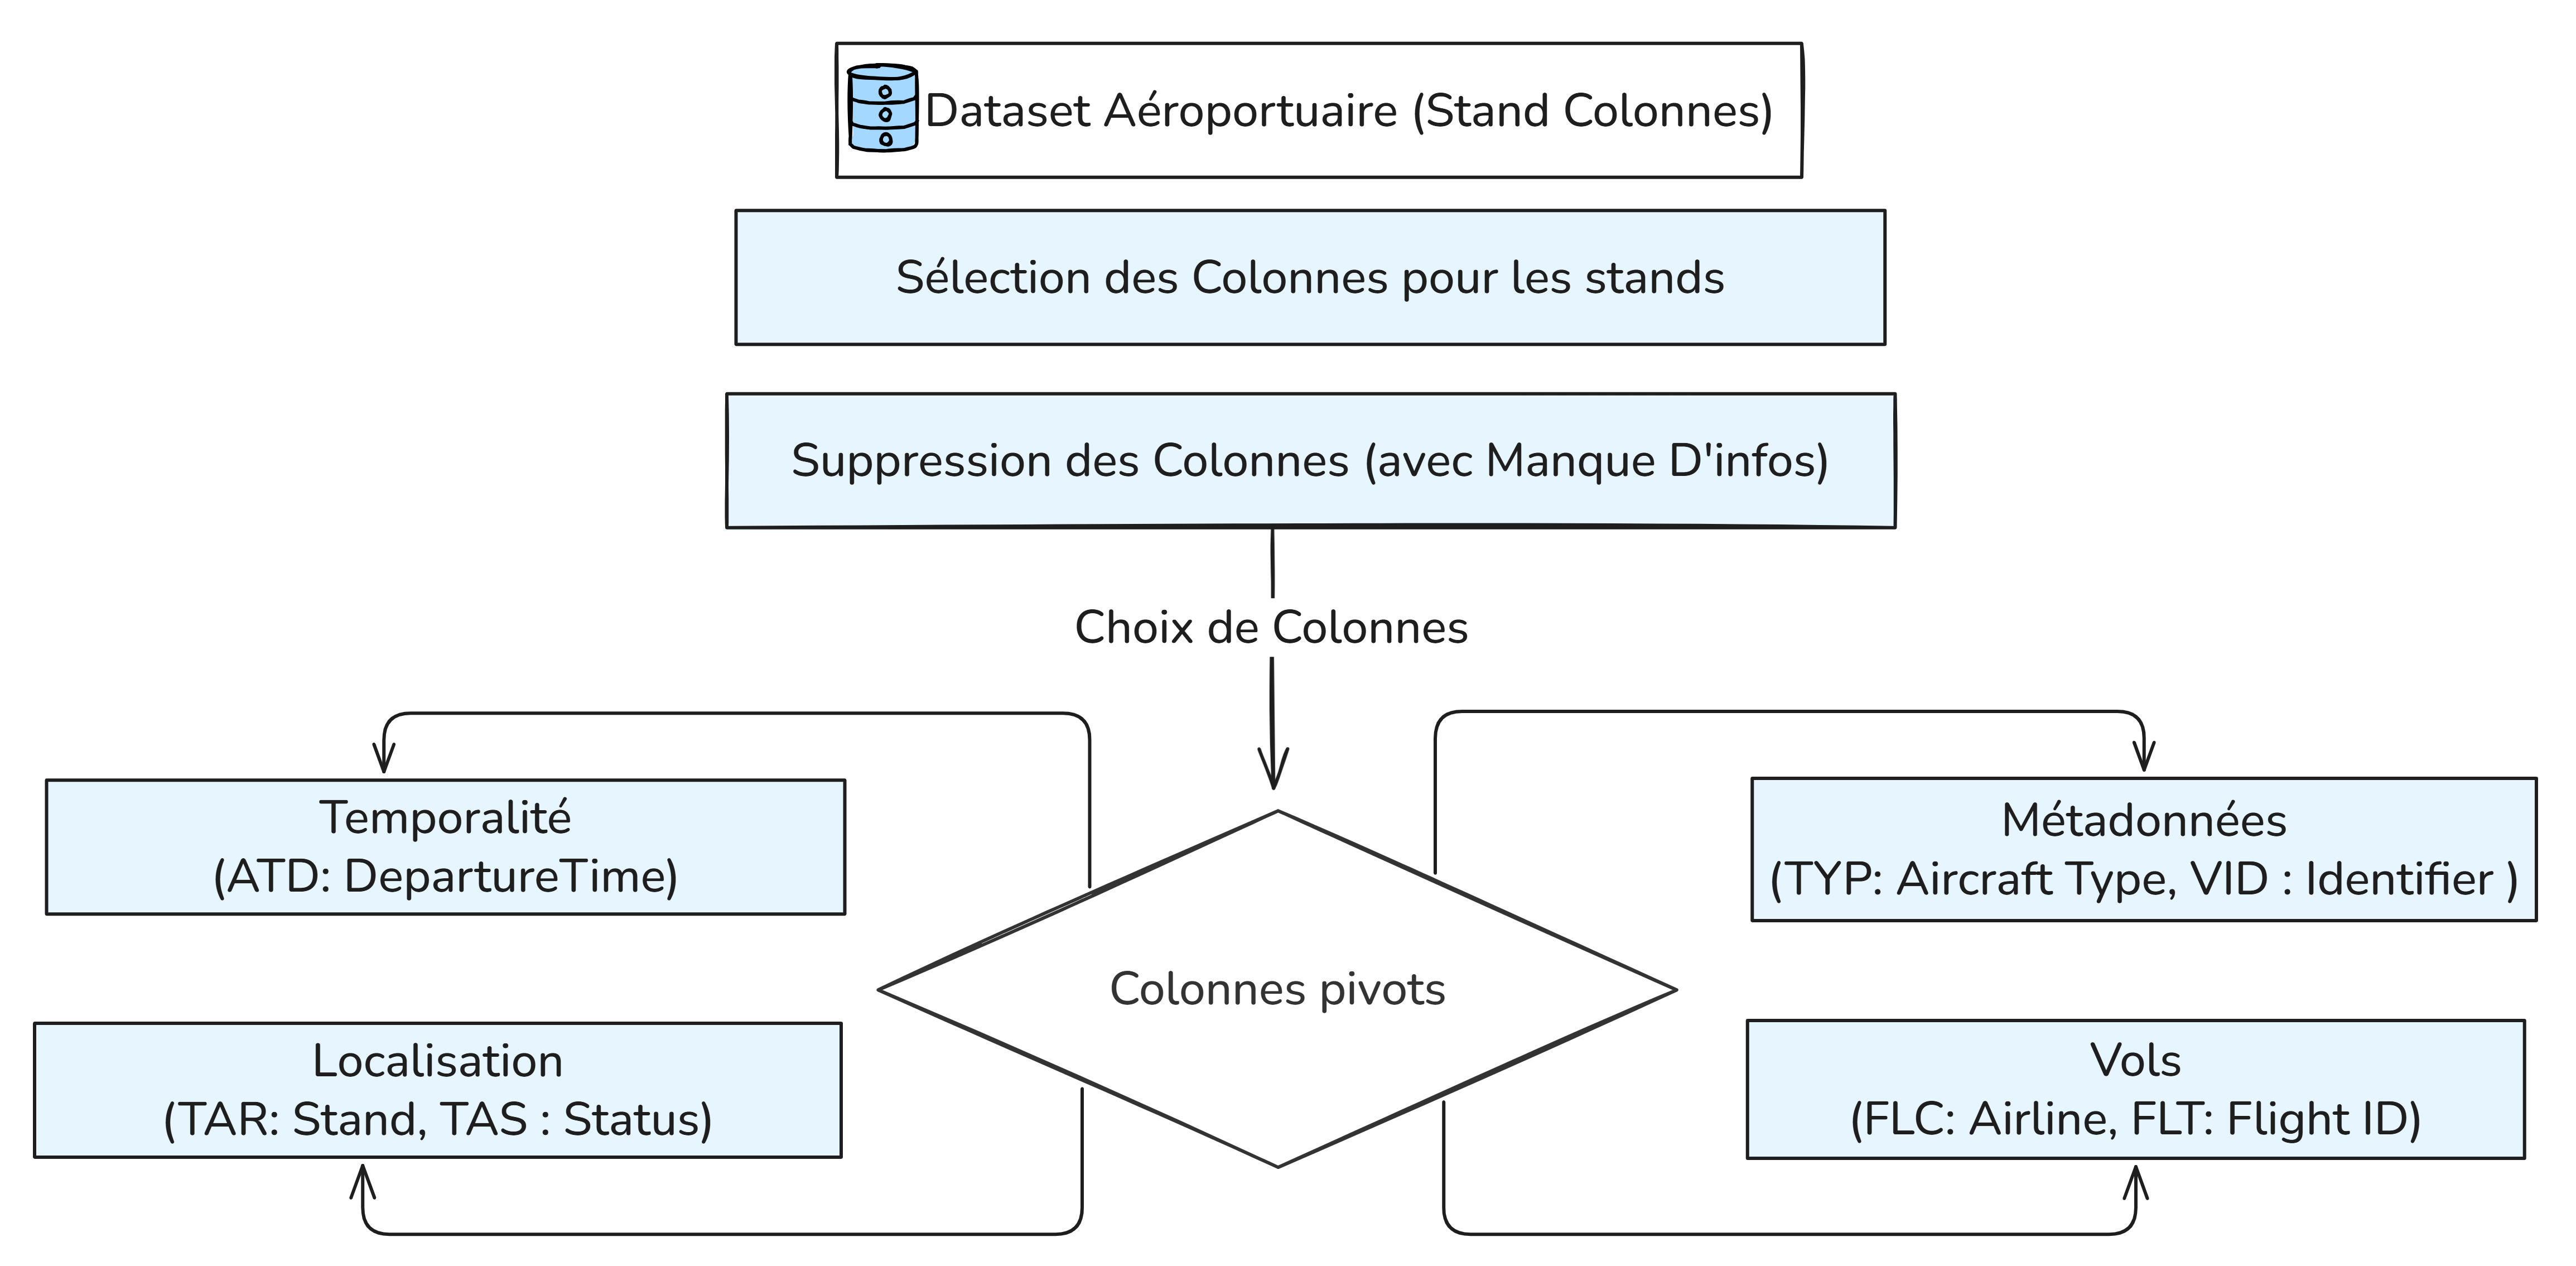
\includegraphics[width=0.8\linewidth]{assets/dataset/DataChart.jpg}
	\caption{Sélection des Caractéristiques}
	\label{fig:stand-selection}
\end{figure}

\subsubsection{Analyse des données}

Après avoir effectué la sélection des caractéristiques et le prétraitement, nous avons adopté une démarche analytique structurée, illustrée dans la figure~\ref{fig:stand-analysis-flow}. L’analyse a débuté par une vue d’ensemble des taux d’occupation des stands sur une période donnée, permettant d’identifier les tendances générales ainsi que le niveau d’utilisation de la capacité.

Pour une compréhension plus fine, l’analyse a ensuite été affinée en isolant chaque compagnie aérienne. Cela a permis de calculer les taux d’occupation des stands dédiés à chaque compagnie. Par la suite, nous avons évalué l’utilisation des stands par type d’avion au sein de chaque compagnie, afin de dégager des schémas liés à la catégorie d’appareil et à l’usage des infrastructures.

\begin{figure}[H]
	\centering
	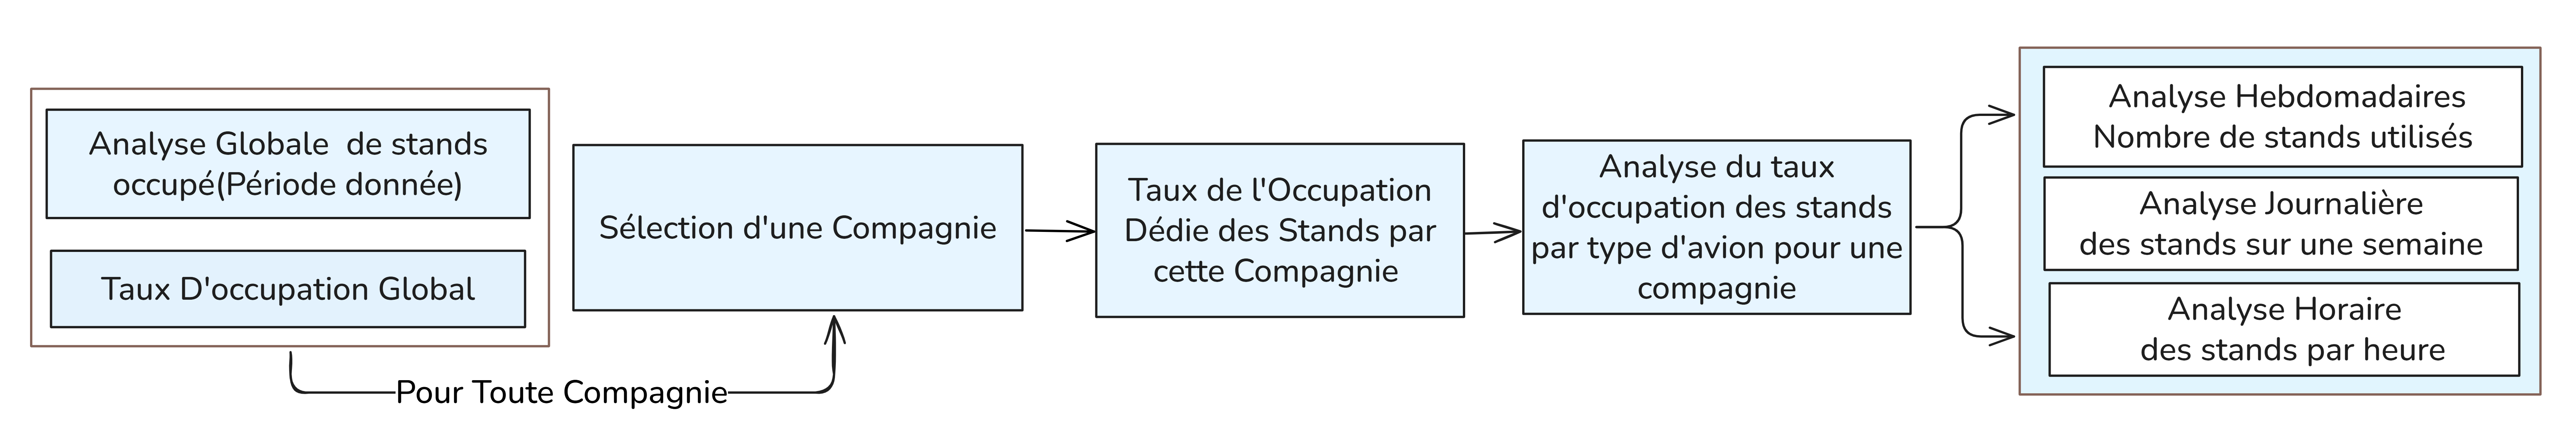
\includegraphics[width=1\linewidth]{assets/dataset/standAnalyse.png}
	\caption{Diagramme de Flux d'Analyse des Données}
	\label{fig:stand-analysis-flow}
\end{figure}


\begin{enumerate}
	\item \textbf{Analyse globale de l’occupation des stands}
	
	\hspace{0.5cm} Cette section présente une analyse approfondie de l’utilisation des postes de stationnement de l’aéroport sur une période de deux mois. L’objectif est d’identifier les schémas d’occupation en fonction des créneaux horaires et des compagnies aériennes, ainsi que d’évaluer l’efficacité de l’allocation des ressources selon les types d’avions.
	
	\begin{figure}[H]
		\centering
		\begin{subfigure}[t]{0.49\textwidth}
			\centering
			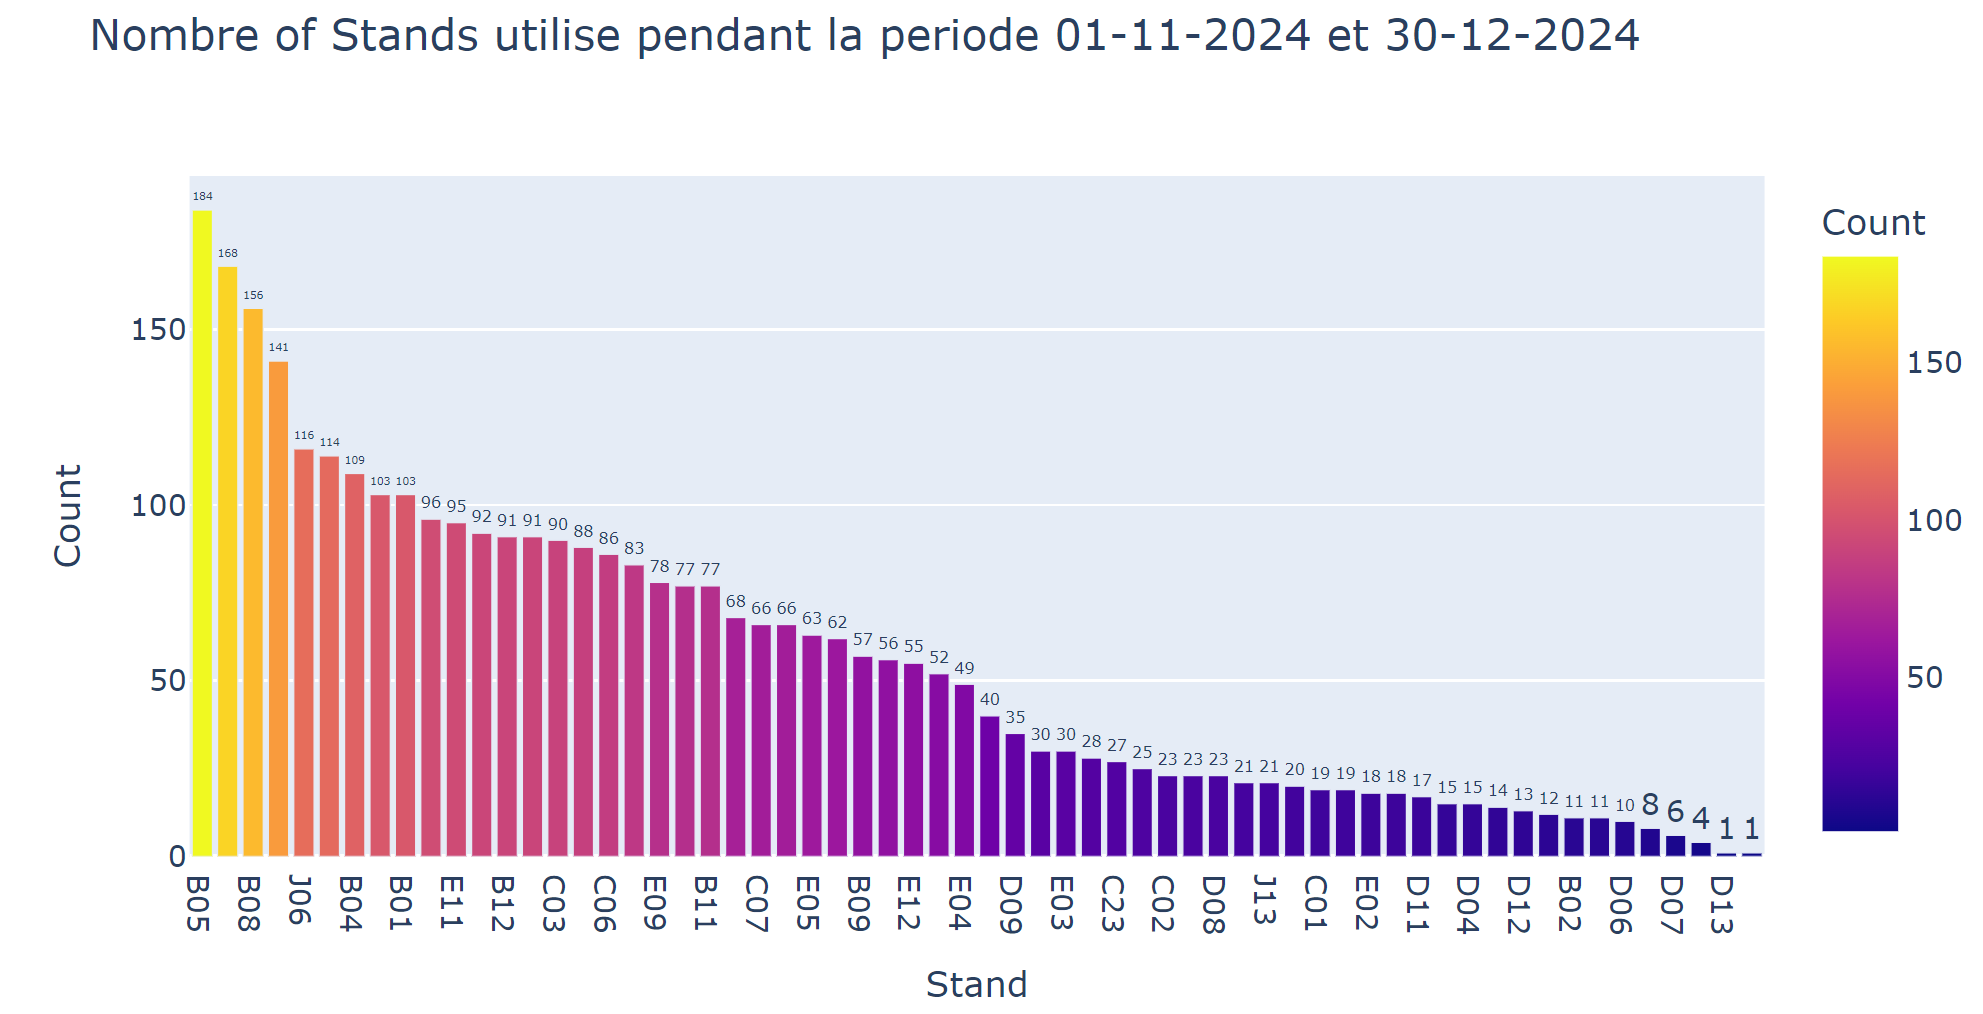
\includegraphics[width=\linewidth]{assets/dataset/Global_Satnds.png}
			\caption{Distribution de l'utilisation des stands sur la période d'étude (2 mois)}
			\label{fig:global_stands_utilization}
		\end{subfigure}
		\hfill
		\begin{subfigure}[t]{0.49\textwidth}
			\centering
			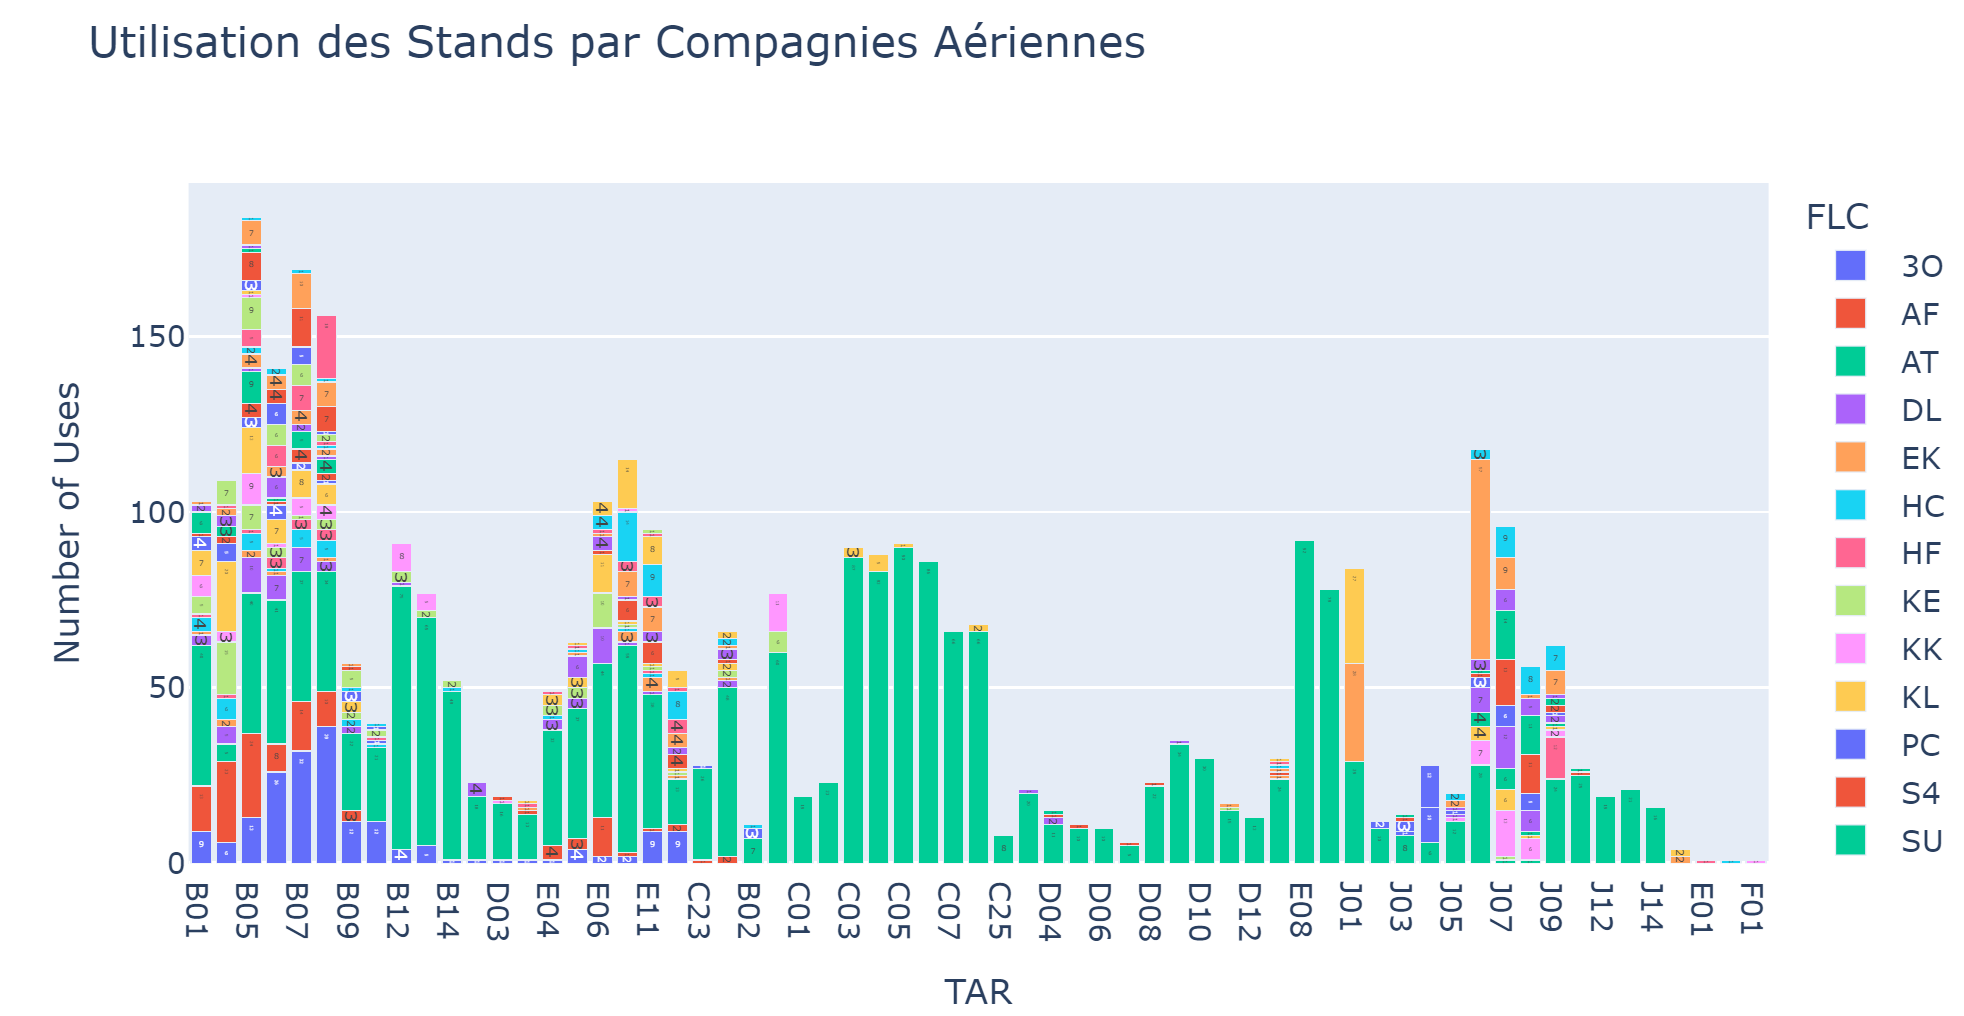
\includegraphics[width=\linewidth]{assets/dataset/Divsersity.png}
			\caption{Diversité des compagnies aériennes par stand}
			\label{fig:diversity_by_stand}
		\end{subfigure}
		\caption{Diversité des compagnies aériennes par stand}
		
	\end{figure}
	
	

	\hspace{0.5cm} La \textbf{figure \ref{fig:global_stands_utilization}} met en évidence une répartition hétérogène de l’occupation des stands. Certaines positions de stationnement présentent des taux d’occupation nettement supérieurs à la moyenne, notamment :  
	\textbf{B05 (184), B07 (168), B08 (156), B06 (141) et J06 (116).}
	
	À l’inverse, certains stands sont très peu utilisés :  
	\textbf{D07 (6), J15 (4), D13 (1) et E01 (1).}
L’emplacement physique de ces stands sur le plan de l’aéroport est présenté en \textbf{annexe} (voir Figure~\ref{fig:plan}).

	\hspace{0.5cm} La \textbf{figure de droite~\ref{fig:diversity_by_stand}} illustre la diversité des compagnies aériennes par stand. Elle montre que certains emplacements accueillent une large variété de transporteurs. Par exemple, le \textbf{stand B01} est utilisé par au moins \textbf{cinq compagnies différentes} (\ac{3O}, AF, \ac{AT}, DL, EK) avec des fréquences variables.
	
	\item \textbf{Utilisation des stands par compagnie aérienne et type d’avion}
	
	\hspace{0.5cm} Cette section examine en détail l’utilisation des stands, en se concentrant sur deux aspects : la répartition par compagnie aérienne et par type d’avion. L’objectif est d’identifier les principaux utilisateurs des infrastructures aéroportuaires et de comprendre la répartition des types d’appareils.
	
	\begin{figure}[H]
		\centering
		\begin{minipage}[b]{0.52\linewidth}
			\centering
			\includegraphics[width=\linewidth]{assets/dataset/compagnie.png}
			\caption{Répartition de l'occupation des stands par compagnie aérienne}
			\label{fig:airline_occupation}
		\end{minipage}
		\hfill
		\begin{minipage}[b]{0.45\linewidth}
			\centering
			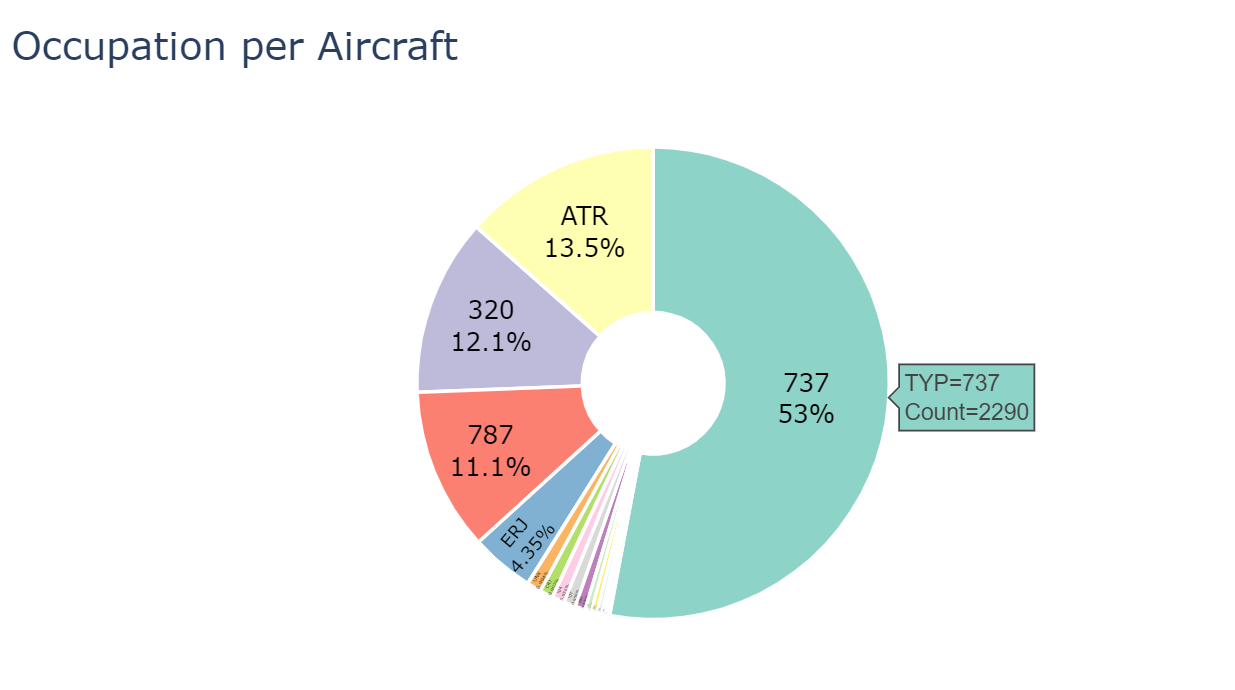
\includegraphics[width=\linewidth]{assets/dataset/AircraftOccupation.png}
			\caption{Répartition de l’occupation par type d’avion}
			\label{fig:AicraftOccupation}
		\end{minipage}
	\end{figure}
	
\hspace{0.5cm} \textbf{La figure de gauche~\ref{fig:airline_occupation}} révèle une prédominance marquée des transporteurs nationaux marocains. Notamment, \ac{AT} représente une part importante de l’utilisation des stands.

\begin{table}[H]
	\centering
	\renewcommand{\arraystretch}{0.8} % réduit l'espacement vertical
	\caption{Principales compagnies aériennes selon le nombre d’utilisations des stands}
	\begin{tabular}{l l c}
		\toprule
		\textbf{Code IATA} & \textbf{Compagnie} & \textbf{Nombre d’utilisations} \\
		\midrule
		AT & Royal Air Maroc & 3361 \\
		3O & Air Arabia Maroc & 221 \\
		AF & Air France & 122 \\
		AC & Air Canada & 47 \\
		6E & IndiGo & 29 \\
		\bottomrule
	\end{tabular}
	\label{tab:top_airlines}
\end{table}


\hspace{0.5cm} Cette distribution confirme la domination de \ac{AT}, suivie par \ac{3O}, indiquant que les compagnies nationales sont les principaux utilisateurs des infrastructures aéroportuaires.

\hspace{0.5cm} \textbf{La figure de droite~\ref{fig:AicraftOccupation}} montre que trois types d’avions dominent les opérations aéroportuaires : le Boeing 737 (46,6 \%), l’Airbus A320 (16,7 \%) et l’ATR (12,2 \%). Ensemble, ils représentent plus de 75 \% des mouvements totaux. Des appareils comme le Boeing 787 (11,9 \%) et l’Embraer ERJ (4,6 \%) sont modérément utilisés, tandis que d’autres types sont marginalement présents.

\item \textbf{Analyse selon trois niveaux de fréquence}

\hspace{0.5cm} L’étude des tendances temporelles de l’occupation des stands permet d’identifier les schémas cycliques et saisonniers qui caractérisent les opérations aéroportuaires. Cette analyse multiniveau offre une compréhension détaillée des variations de la demande en stands au fil du temps.

\begin{figure}[H]
	\centering
	\begin{minipage}[b]{0.49\linewidth}
		\centering
		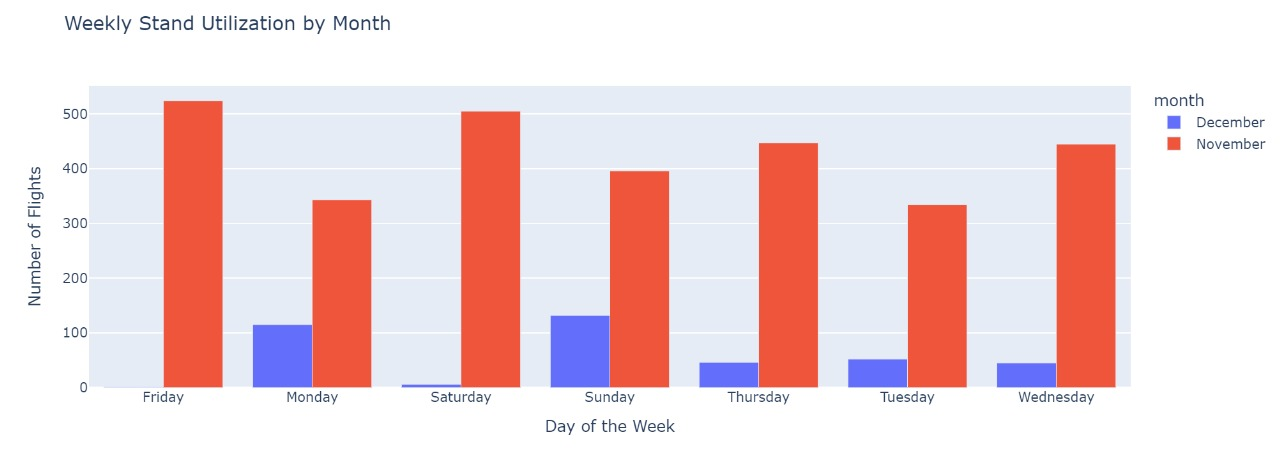
\includegraphics[width=\linewidth]{assets/dataset/WeeklyOccupation.jpg}
		\caption{Variation hebdomadaire de l’occupation des stands}
		\label{fig:WeeklyOccupation}
	\end{minipage}
	\hfill
	\begin{minipage}[b]{0.49\linewidth}
		\centering
		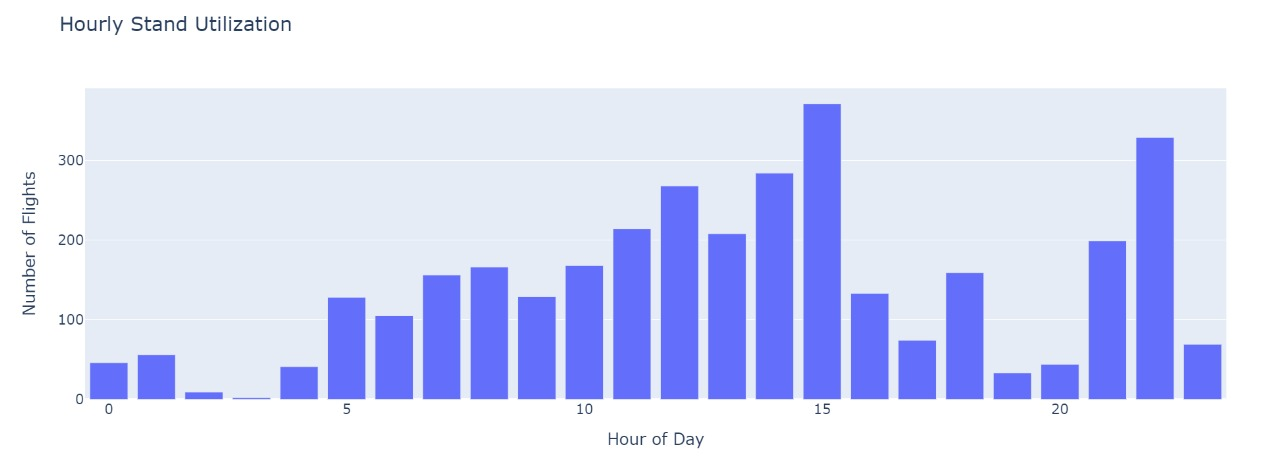
\includegraphics[width=\linewidth]{assets/dataset/HourlyOccupation.jpg}
		\caption{Variation horaire de l’occupation des stands}
		\label{fig:HourlyOccupation}
	\end{minipage}
\end{figure}

\hspace{0.5cm} \textbf{Gauche : Analyse hebdomadaire \ref{fig:WeeklyOccupation}}
Cette analyse met en évidence des tendances hebdomadaires et saisonnières d’occupation. En novembre, les pics sont observés le vendredi (524 vols), samedi (505) et dimanche (396), indiquant une forte activité en fin de semaine. En décembre, l’activité diminue globalement, avec des pics plus modestes le dimanche (132) et le lundi (115).  


\hspace{0.5cm} \textbf{Droite : Analyse horaire \ref{fig:HourlyOccupation}}
Cette analyse révèle que l’activité est concentrée entre 5h et 16h, avec des pics à 15h (371 vols), 14h (284) et un second à 22h (329), probablement lié aux départs tardifs. L’activité est minimale entre 2h et 4h du matin.


\end{enumerate}





\subsection{Analyse des retards}

L’analyse des retards représente un volet important de notre étude, car elle permet de mieux comprendre les sources de perturbations et leur impact sur la planification des stands.

Comme illustré dans la Figure~\ref{fig:retard_flowchart}, cette analyse débute par un prétraitement des données, visant à nettoyer, filtrer et structurer les informations relatives aux retards. Ensuite, plusieurs visualisations globales sont produites.

Par ailleurs, nous avons approfondi l’étude en catégorisant les retards selon différents axes :

\begin{itemize}
\item Retards par compagnie aérienne.
\item Niveau de criticité par compagnie.
\item Retards en fonction du stand utilisé.
\item Retards selon la taille de l'avion.
\end{itemize}

\begin{figure}[H]
\centering
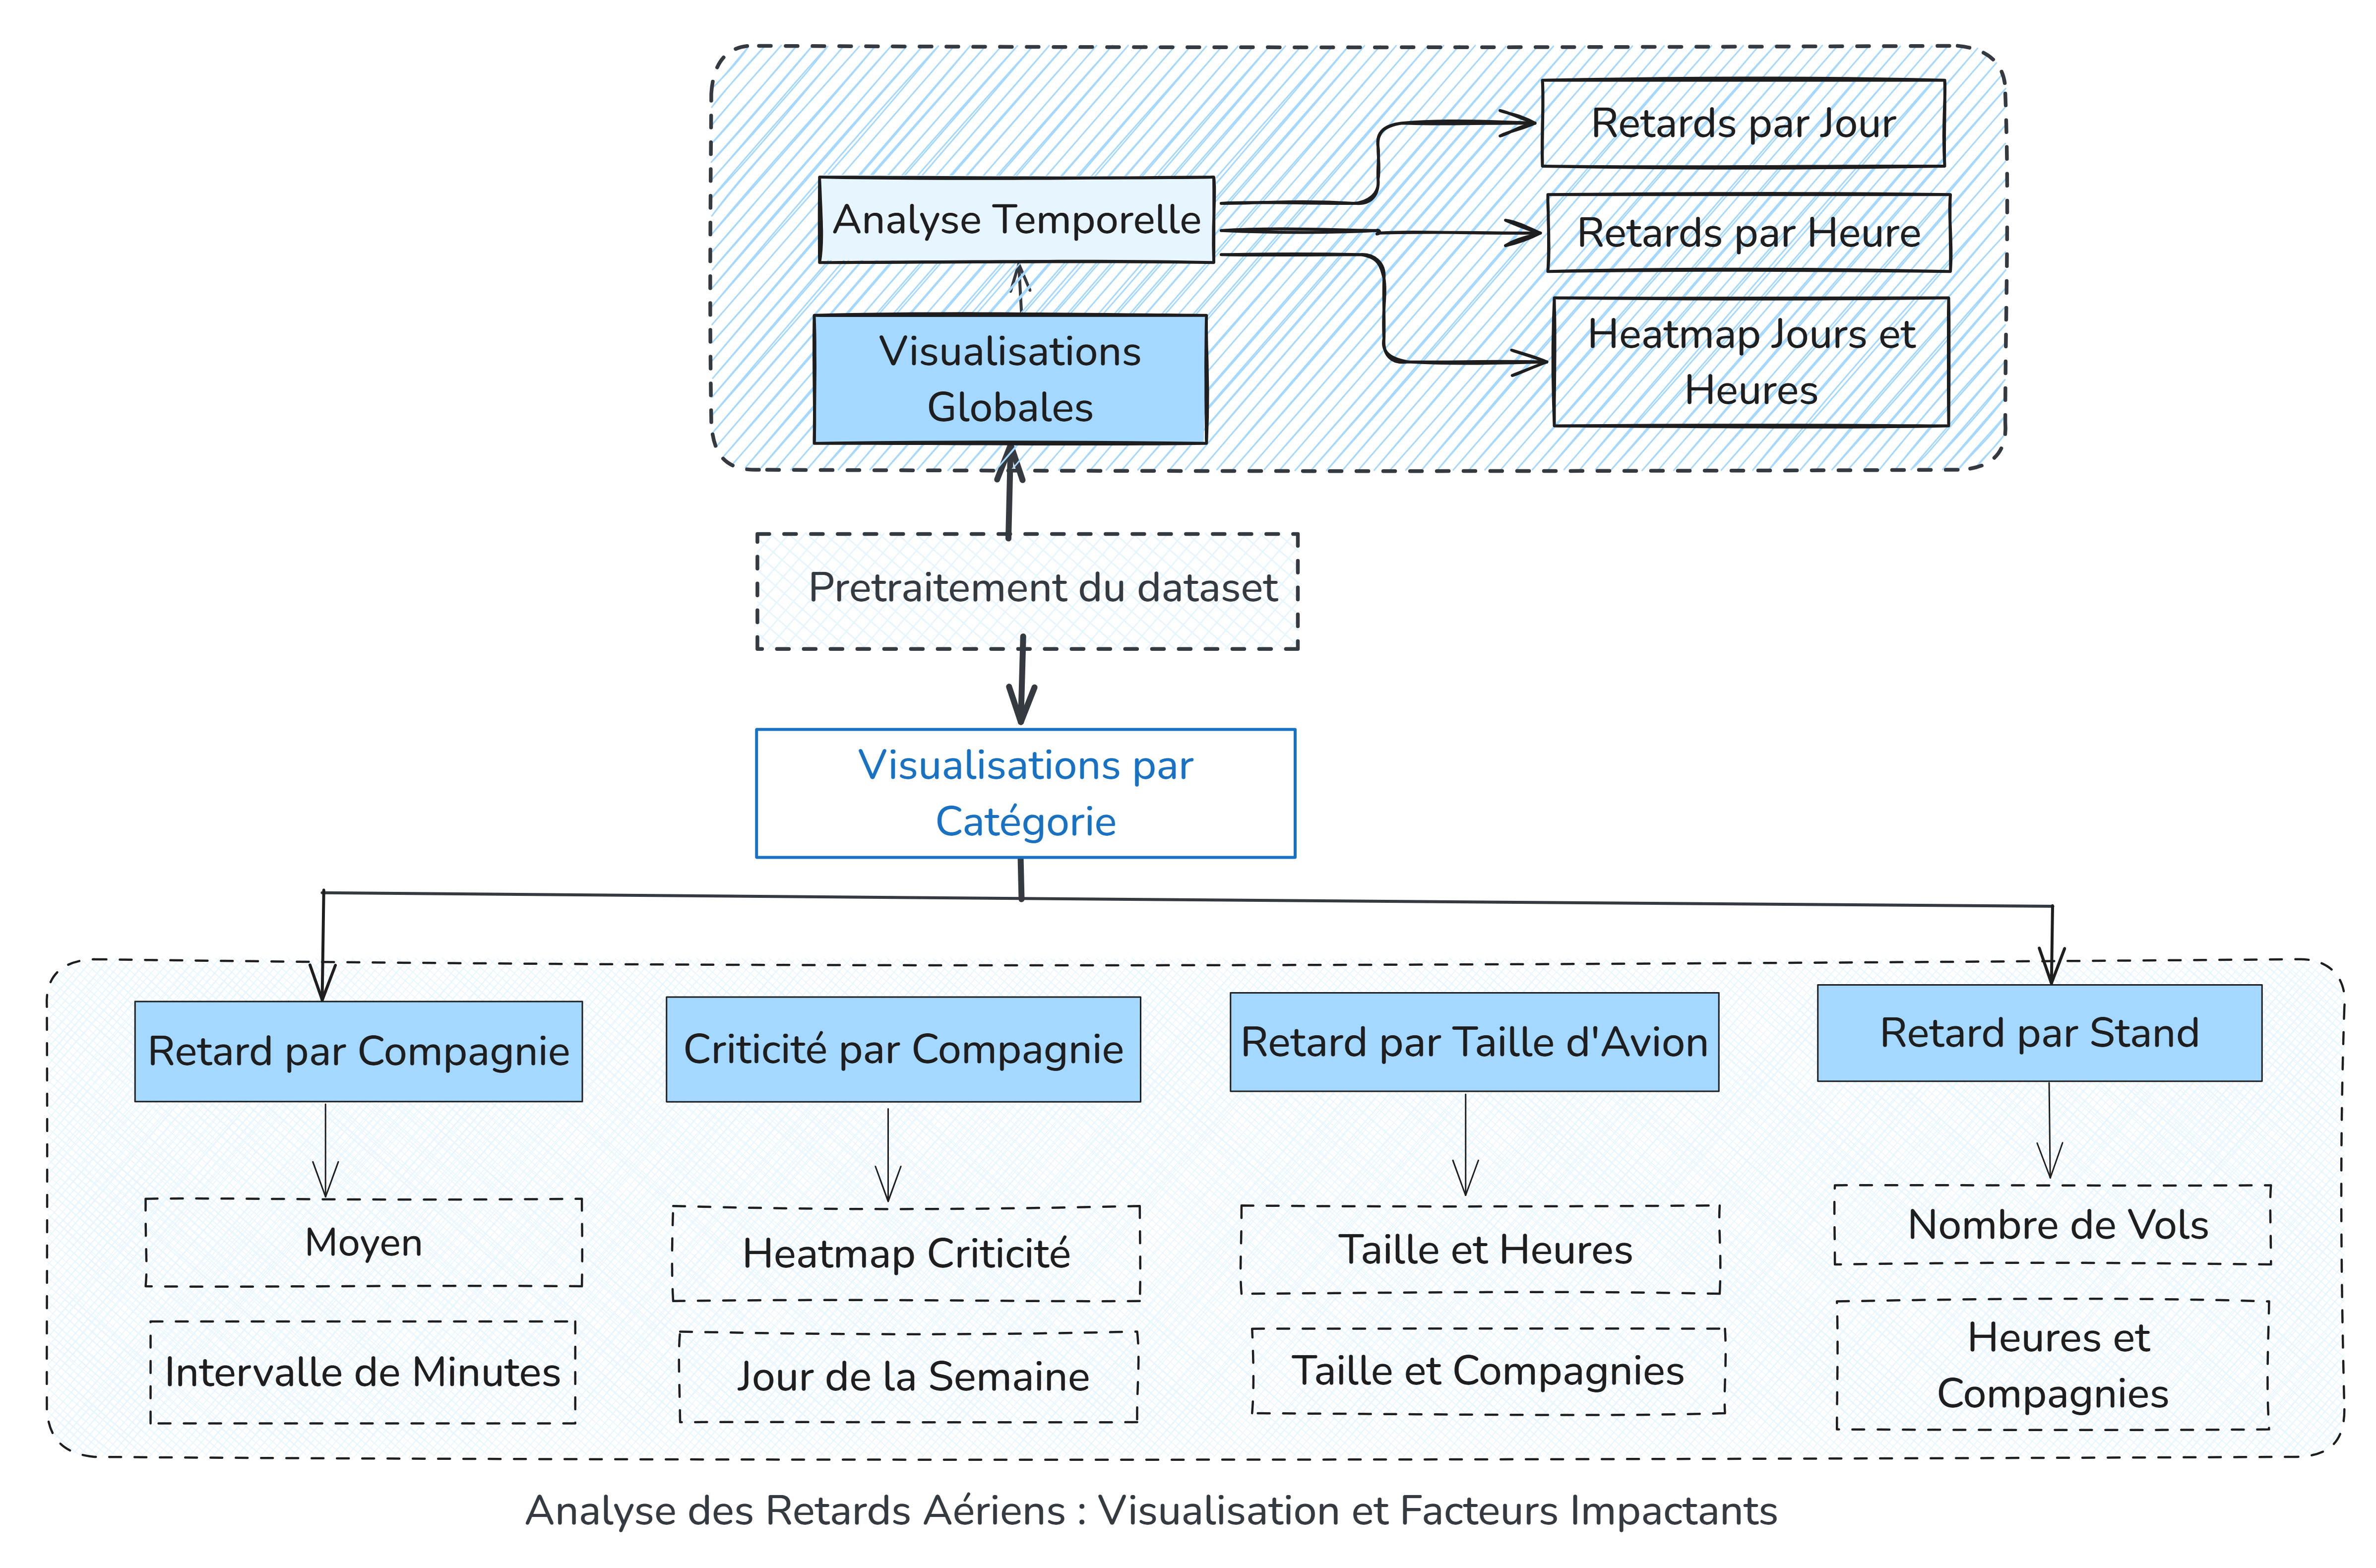
\includegraphics[width=0.9\linewidth]{assets/dataset/flowchartRetard.png}
\caption{Flowchart de l'analyse des retards}
\label{fig:retard_flowchart}
\end{figure}
Les résultats obtenus permettent d’identifier les sources potentielles de saturation ou de mauvaise allocation des ressources aéroportuaires, et servent de base pour générer un dataset optimisé destiné à l’apprentissage de notre modèle de prédiction et d’affectation des stands.

\subsubsection{Prétraitement du dataset}
Cette section décrit les \textbf{étapes clés du prétraitement} effectuées sur notre dataset pour l’analyse des retards aériens.
\begin{figure}[H]
\centering
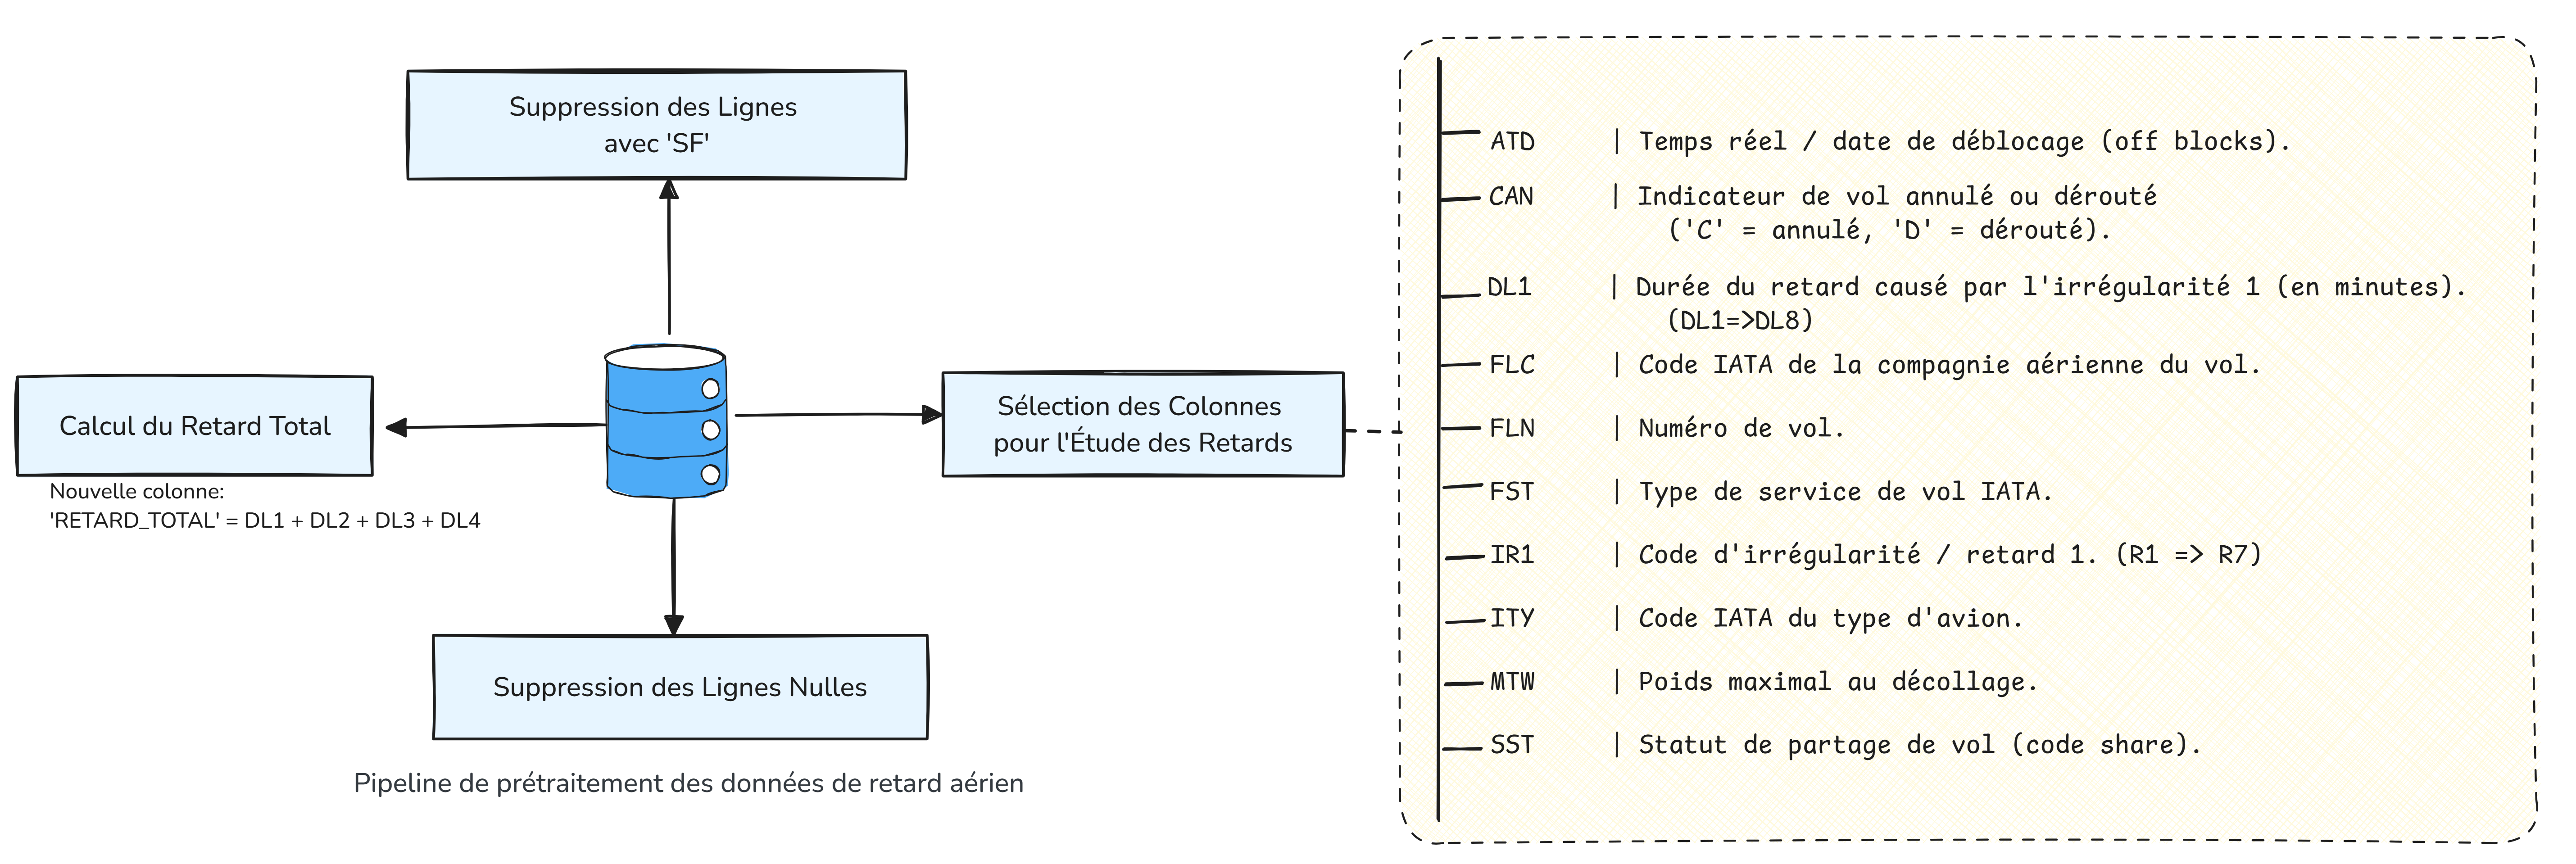
\includegraphics[width=0.8\linewidth]{assets/dataset/pretraitement.png}
\caption{Les étapes de prétraitement du dataset}
\label{fig:pretraitementData}
\end{figure}

Ces étapes ont été définies à partir d’une \textbf{étude approfondie du document de référence} fourni par le client, documentant en détail les \textbf{485 colonnes} disponibles dans le fichier source. L’objectif était de filtrer et structurer les données de manière à isoler les variables les plus pertinentes pour l’étude des retards.

\vspace{0.5em}
\textbf{1. Sélection stratégique des colonnes}

Sur la base du document PDF fourni par le client, une sélection des colonnes a été effectuée pour l’analyse des retards. Les variables retenues incluent :

\begin{itemize}
\item \texttt{ATD}: Représente l’heure réelle de départ du vol, essentielle pour le calcul précis du retard.

\item \texttt{CAN} : Indicateur précisant si un vol a été annulé ou dérouté.

\item \texttt{IR1} à \texttt{IR8} : Ensemble de colonnes représentant les causes détaillées des retards (problèmes techniques, météo, trafic, etc.) sous forme de codes.

\item \texttt{DL1} à \texttt{DL8} : Durée du retard (en minutes) associée à chaque cause pour un vol donné.

\item \texttt{MTW}: Poids maximal autorisé pour le décollage de l’avion.

\item \texttt{SST} : Indicateur du statut de partage de vol (code-share).
\end{itemize}


\vspace{0.5em}
\textbf{2. Nettoyage des données}

Une fois les colonnes pertinentes sélectionnées, nous avons entrepris un nettoyage du dataset :

\begin{itemize}
\item \textbf{Suppression des lignes incomplètes} : Toutes les entrées contenant des valeurs nulles dans les colonnes.
\item \textbf{Filtrage des vols non pertinents} : En se basant sur l'analyse des vols lors de l’étude initiale, les lignes où
certaines compagnies n’opéraient que des vols en partage de code, sans présence opérationnelle directe ont été écartées.
\end{itemize}

\vspace{0.5em}
\textbf{3. Création de la colonne \texttt{RETARD\_TOTAL}}

D'après les indications fournies par le client, la durée totale de retard correspond à la somme des retards enregistrés. Alors, la variable \texttt{RETARD\_TOTAL} agrège les minutes de retard signalées dans les colonnes \texttt{DL1} à \texttt{DL8}. La formule utilisée est la suivante :

\[
\texttt{RETARD\_TOTAL} = \sum_{i=1}^{8} \texttt{DL}_i
\]




\subsubsection{Visualisations globales}
Des visualisations globales ont été réalisées pour mieux comprendre le comportement du dataset.
\paragraph{Retards par jour et par heure}
\mbox{}\\
La figure \ref{fig:retards_temporels} présente deux visualisations : la première montre le nombre de vols retardés par jour, tandis que la seconde illustre le pourcentage de retards en fonction de l’heure de la journée.
\begin{figure}[H]
\centering
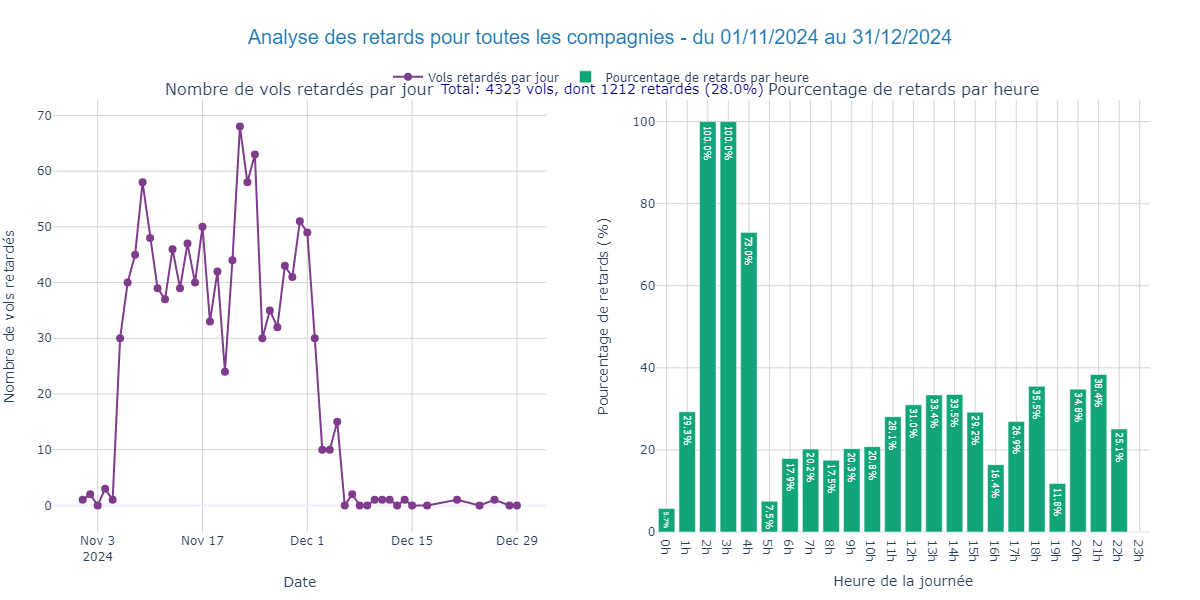
\includegraphics[width=0.9\linewidth]{assets/dataset/parCompagnie.png}
\caption{Analyse temporelle des retards : par jour et par heure}
\label{fig:retards_temporels}
\end{figure}
\vspace{-1em}
Nous analysons la répartition temporelle des vols retardés sur l’ensemble de la période d’étude.Le mois de novembre montre une concentration élevée de retards, avec des pics dépassant 60 vols par jour. La diminution en décembre s'explique par la répartition du trafic aérien où l'\ac{CMN} enregistre moins de vols durant cette période, tandis que l'aéroport de Marrakech devient dominant.

\vspace{-1em}
\paragraph{Analyse des retards par période et par stand}
\mbox{}\\
Cette section présente une double analyse des retards enregistrés entre novembre et décembre 2024, en croisant les données selon les jours/heures et les stands d’affectation.
 \vspace{-1em}
\begin{figure}[H]
	\centering
	\begin{subfigure}[b]{0.5\textwidth}
		\centering
		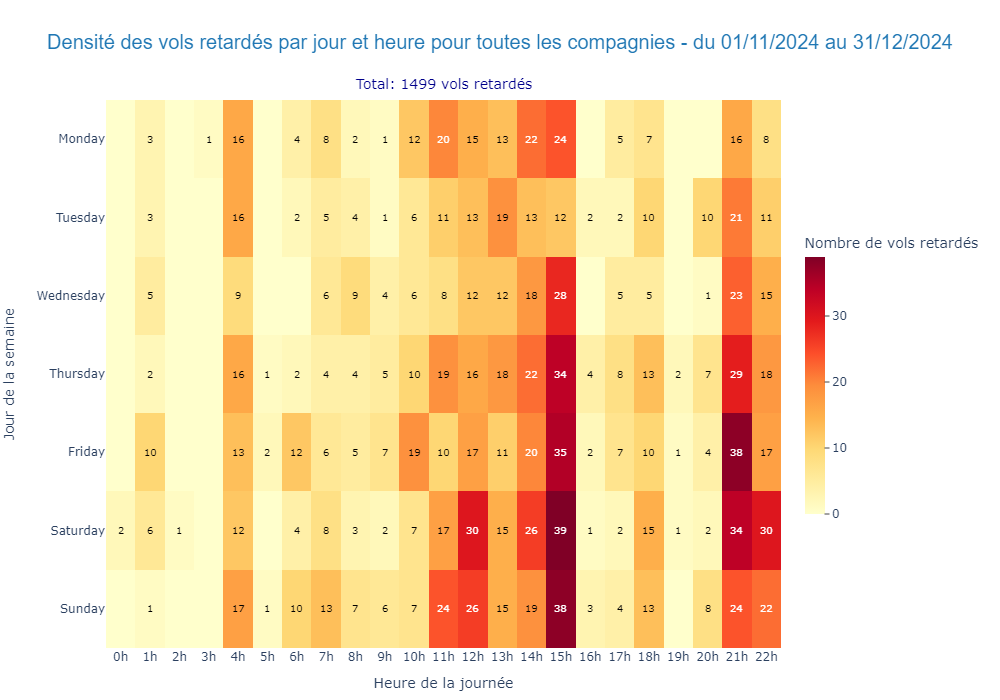
\includegraphics[width=\linewidth]{assets/dataset/parComapgnie2.png}
		\caption{Retards par jour de la semaine et heure (Nov–Déc 2024)}
		\label{fig:heatmap_retards}
	\end{subfigure}
	\hfill
	\begin{subfigure}[b]{0.48\textwidth}
		\centering
		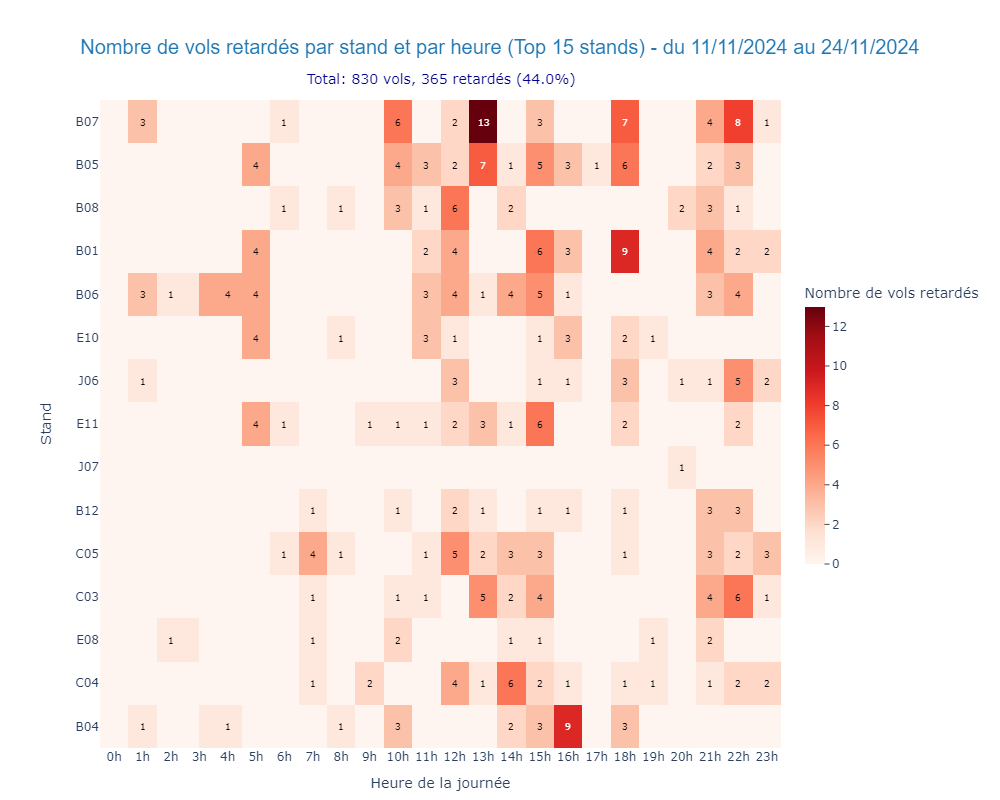
\includegraphics[width=\linewidth]{assets/dataset/parStand.png}
		\caption{Retards par stand et heure (11–24 nov. 2024)}
		\label{fig:retard_stand}
	\end{subfigure}
	\caption{Analyse croisée des retards selon différentes dimensions}
\end{figure}
 \vspace{-1em}
Les résultats montrent des pics de retards :
\begin{itemize}[leftmargin=1.5em]
	\item Le \textbf{vendredi}, le \textbf{samedi après-midi} et le \textbf{dimanche soir}, en lien avec le trafic hebdomadaire.
	\item Aux stands \textbf{B07}, \textbf{B05} et \textbf{B01}, surtout entre \textbf{11h et 16h}, où l’activité est particulièrement dense.
\end{itemize}
 \vspace{-1em}
\subsubsection{Visualisations par catégorie}
 \vspace{-0.5em}
Des visualisations par catégorie ont été réalisées pour approfondir l’analyse. 
\begin{enumerate}
	\item \textbf{Retard par compagnie}
	
	Cette section explore la criticité des retards selon les compagnies aériennes, les jours de la semaine et les créneaux horaires.
	
	\begin{figure}[H]
		\centering
		\begin{subfigure}[b]{0.5\linewidth}
			\centering
			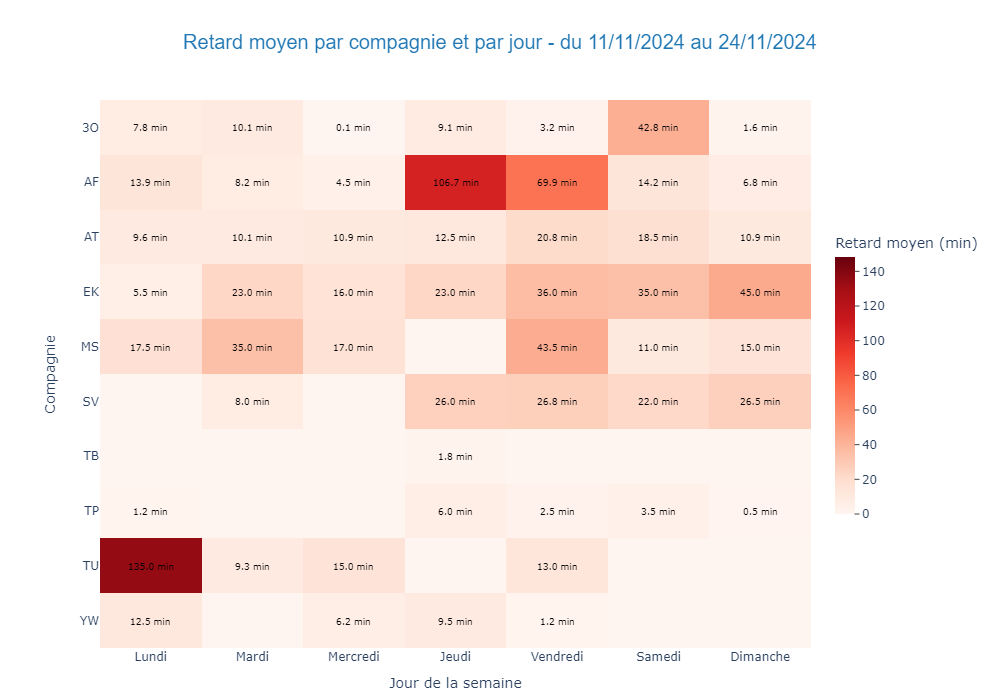
\includegraphics[width=\linewidth]{assets/dataset/parCompagnie3.png}
			\caption{Retard moyen (en min) par compagnie et par jour}
			\label{fig:retard_par_jour}
		\end{subfigure}
		\hfill
		\begin{subfigure}[b]{0.48\linewidth}
			\centering
			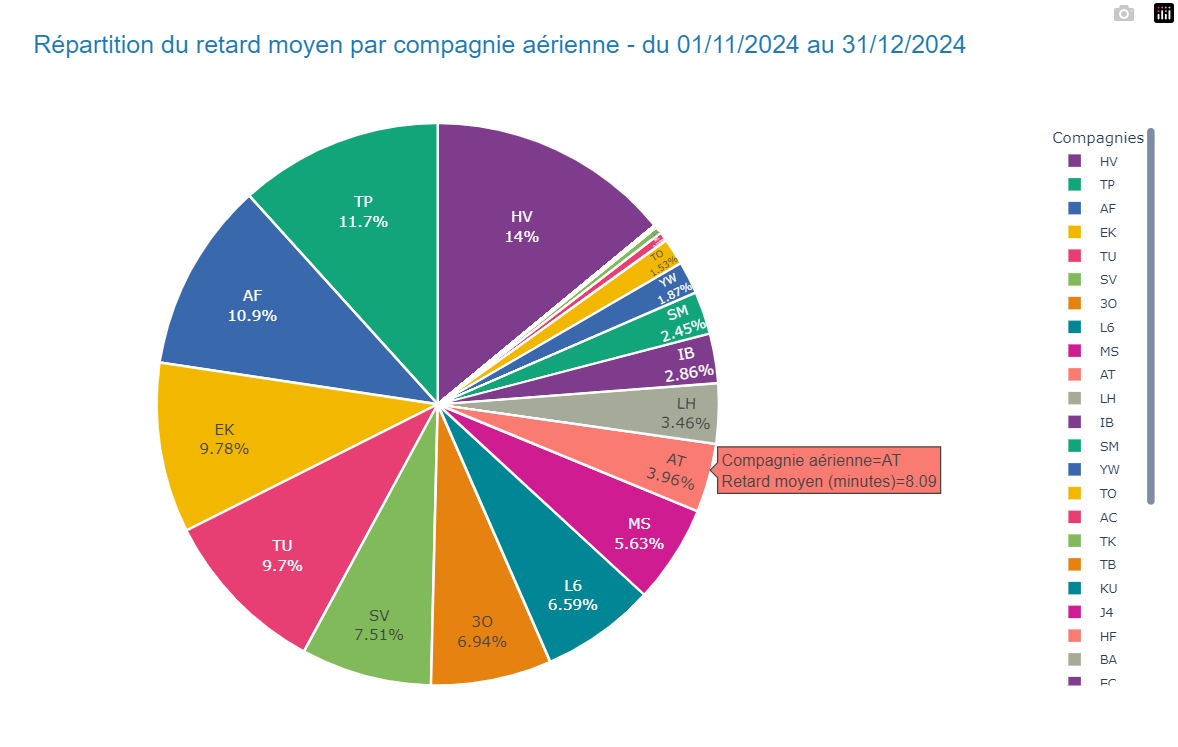
\includegraphics[width=\linewidth]{assets/dataset/parCompagnie4.png}
			\caption{Répartition globale du retard moyen par compagnie}
			\label{fig:repartition_retard}
		\end{subfigure}
		\caption{Visualisations des retards moyens selon les compagnies aériennes}
		\label{fig:retards_par_compagnie}
	\end{figure}
\vspace{-1.6em}
La heatmap \ref{fig:retard_par_jour} montre par exemple un pic critique pour \textbf{TU (Tunisair)} le lundi (135 min). D'autres compagnies comme \textbf{AF} ou \textbf{MS (EgyptAir)} présentent également des retards élevés.  
Le graphique circulaire (\ref{fig:repartition_retard}) indique que \textbf{Transavia} enregistre le retard moyen le plus élevé (14\%), tandis que \textbf{\ac{AT}} affiche un retard moyen faible (8 min).
 \vspace{-1em}
\paragraph{Criticité par jour et par heure}  

 \vspace{-0.5em}
Cette analyse croise les compagnies, jours de semaine et horaires afin d’identifier les périodes les plus sensibles.  
 \vspace{-1em}
\begin{figure}[H]
	\centering
	\begin{subfigure}[b]{0.48\linewidth}
		\centering
		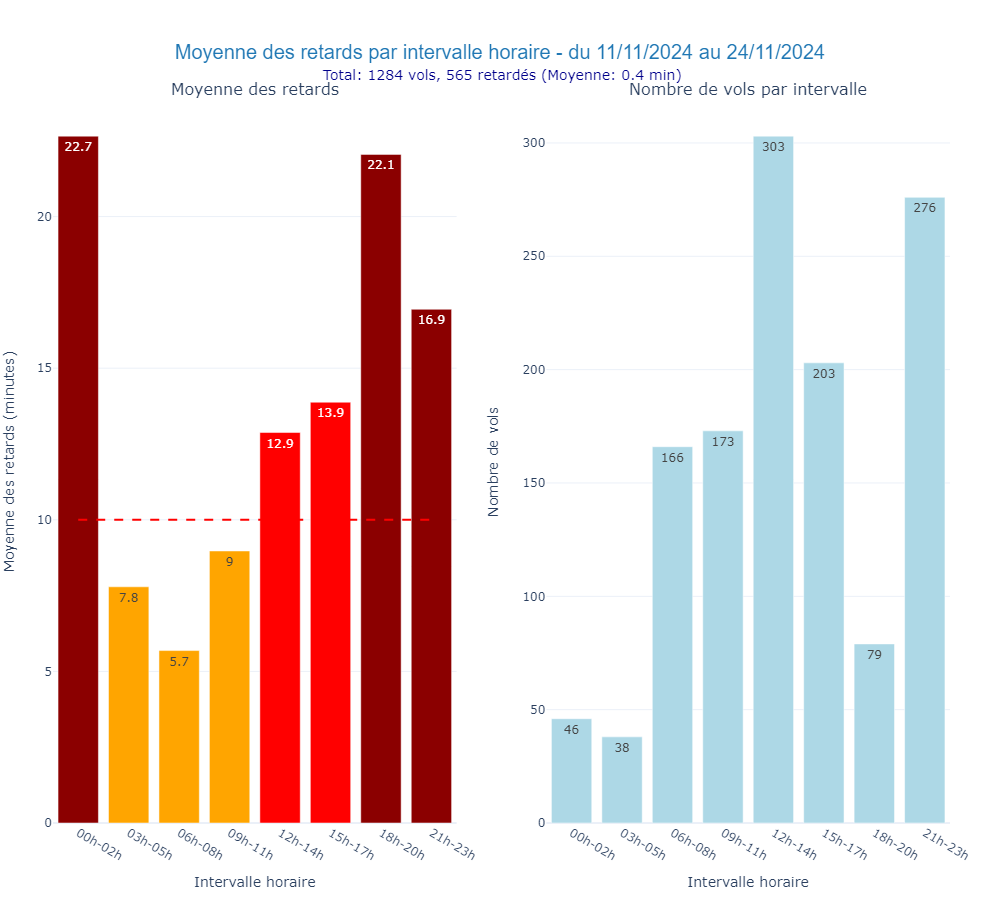
\includegraphics[width=\linewidth]{assets/dataset/parCrticite.png}
		\caption{Retard moyen par tranche horaire}
		\label{fig:retard_moyen_jour}
	\end{subfigure}
	\hfill
	\begin{subfigure}[b]{0.48\linewidth}
		\centering
		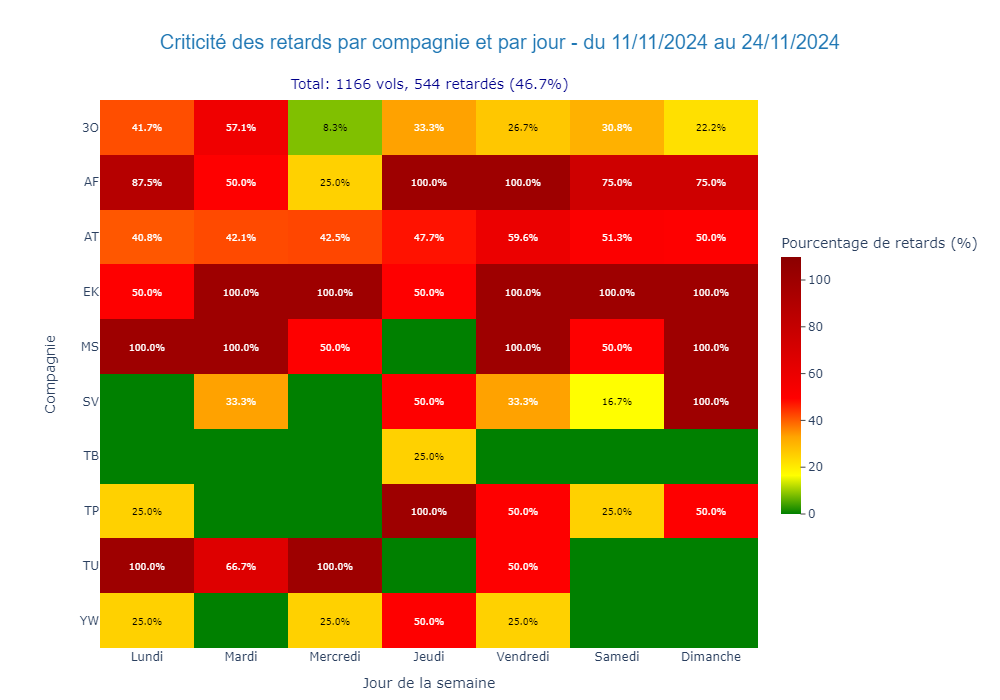
\includegraphics[width=\linewidth]{assets/dataset/parCriticite2.png}
		\caption{Retard moyen (en min) par compagnie et par jour}
		\label{fig:retard_par_heure}
	\end{subfigure}
\end{figure}

Les retards sont importants pour \textbf{TU} le lundi (135 min), ainsi que pour \textbf{AF}, \textbf{\ac{AT}}, et \textbf{MS} en milieu de semaine.  
Les pics horaires se situent entre \textbf{00h–02h} et \textbf{21h–23h} (\ref{fig:retard_par_heure}).

	
	\item \textbf{Retards selon la taille des avions}
	
	L’analyse s’appuie sur le \texttt{MTW} (poids maximal au décollage) pour estimer la taille des avions.
	
	\begin{itemize}
		\item \textbf{Small} : moins de 7 000 kg
		\item \textbf{Medium} : entre 7 000 et 136 000 kg
		\item \textbf{Large} : entre 136 000 et 250 000 kg
		\item \textbf{Super} : plus de 250 000 kg
	\end{itemize}
	 \vspace{-0.7em}
	\begin{figure}[H]
		\centering
		\begin{subfigure}[b]{0.49\linewidth}
			\centering
			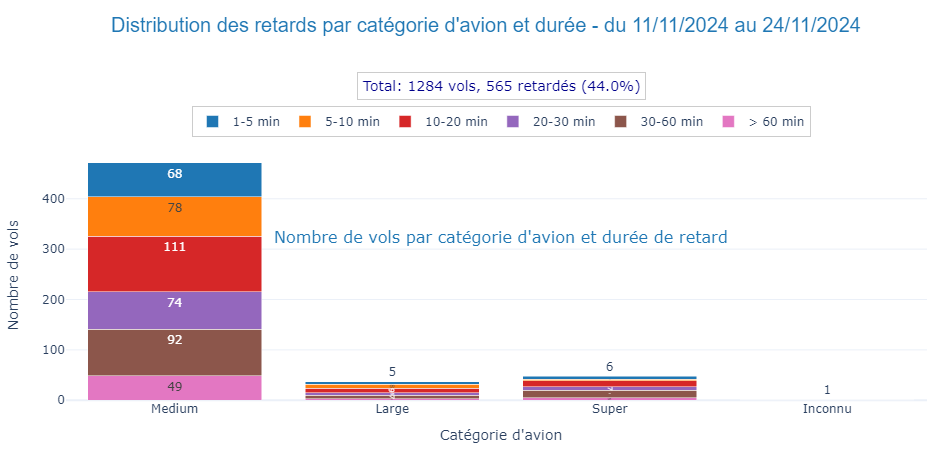
\includegraphics[width=\linewidth]{assets/dataset/tailleAvion.png}
			\caption{Retards par durée (catégorie Medium)}
			\label{fig:duree_medium}
		\end{subfigure}
		\hfill
		\begin{subfigure}[b]{0.49\linewidth}
			\centering
			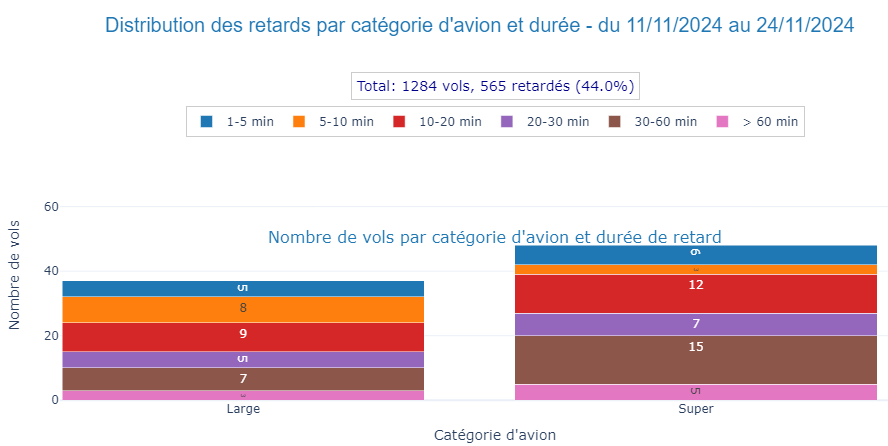
\includegraphics[width=\linewidth]{assets/dataset/tailleAvion2.png}
			\caption{Retards (hors Medium)}
			\label{fig:duree_autres}
		\end{subfigure}
	\end{figure}
	 \vspace{-0.7em}
	Les avions \textbf{Medium} concentrent 479 cas de retard. Deux pics sont notés : entre \textbf{7h–15h} (pic à 13h) et \textbf{21h–22h}.
\end{enumerate}
\vspace{-1.8em}
\section{Préparation des données}
Puisque notre dataset initial est volumineux et que les algorithmes d'affectation nécessitent une base de données optimisée.
\vspace{-1.4em}
\subsection{Fusion des datasets d’arrivée et de départ}
Nous avons opté pour la génération de deux jeux de données distincts : le dataset des vols et celui des stands. Cette génération est basée sur des recherches, notamment l'article de \cite{NilBusquetsTrias}.

Dans un premier temps, nous disposons de deux datasets initiaux : l’un relatif aux arrivées et l’autre aux départs. Chaque vol est donc représenté par une paire — un vol d’arrivée suivi d’un vol de départ, séparés par une période de stationnement. Il est ainsi essentiel de combiner correctement ces deux datasets afin de regrouper les informations d’un vol dans une seule entrée.

Pour effectuer cette fusion, nous nous sommes appuyés sur deux colonnes clés : \texttt{VID}, qui représente un identifiant unique pour chaque vol, et \texttt{REG}, correspondant à l’immatriculation de l’avion. L'utilisation conjointe de ces deux attributs nous a permis de réaliser une correspondance fiable entre les vols d’arrivée et de départ.

\subsubsection*{Les points bloquants}

Lors du processus de fusion des deux jeux de données (arrivées et départs), plusieurs incohérences et cas particuliers ont été identifiés, constituant ainsi des points bloquants :

\begin{itemize}
	\item Certaines compagnies aériennes apparaissent uniquement dans le dataset des départs (par exemple : \textbf{QS}\footnote{QS : Smartwings (République tchèque)}, \textbf{WT}\footnote{WT : Swiftair (Espagne)}), mais sont absentes du dataset des arrivées.
	\item D'autres compagnies sont présentes dans les arrivées (comme \textbf{V7}\footnote{V7 : Volotea (Espagne)}, \textbf{VY}\footnote{VY : Vueling Airlines (Espagne)}), mais ne figurent pas dans les départs.
	\item Certains vols de départ n’ont pas de correspondance dans les arrivées, ce qui rend la liaison incohérente.
	\item De même, certains vols d’arrivée ne sont liés à aucun vol de départ.
\end{itemize}


Afin de garantir l’intégrité du dataset final, nous avons choisi d’exclure ces cas lors de la fusion. Toutefois, ces anomalies soulèvent des interrogations auxquelles nous n'avons pas encore de réponse. 

\subsection{Génération du dataset des vols}

La première étape dans la création du dataset des vols consiste à sélectionner les colonnes pertinentes. Pour cela, nous avons utilisé à la fois :

\begin{itemize}
	\item des colonnes déjà présentes dans le dataset, telles que : le type d’avion, le numéro d’immatriculation, les heures d’arrivée et de départ, ainsi que le code IATA de la compagnie aérienne ;
	\item des colonnes générées à partir d’analyses préalables, notamment : \texttt{day} (le jour de la semaine), \texttt{classification\_aircraft\_size} (la taille de l’avion, classée en small, medium, large ou super), et \texttt{delay\_severity} (qui représente la sévérité du retard : faible, moyen ou élevé).
\end{itemize}

\begin{figure}[H]
	\centering
	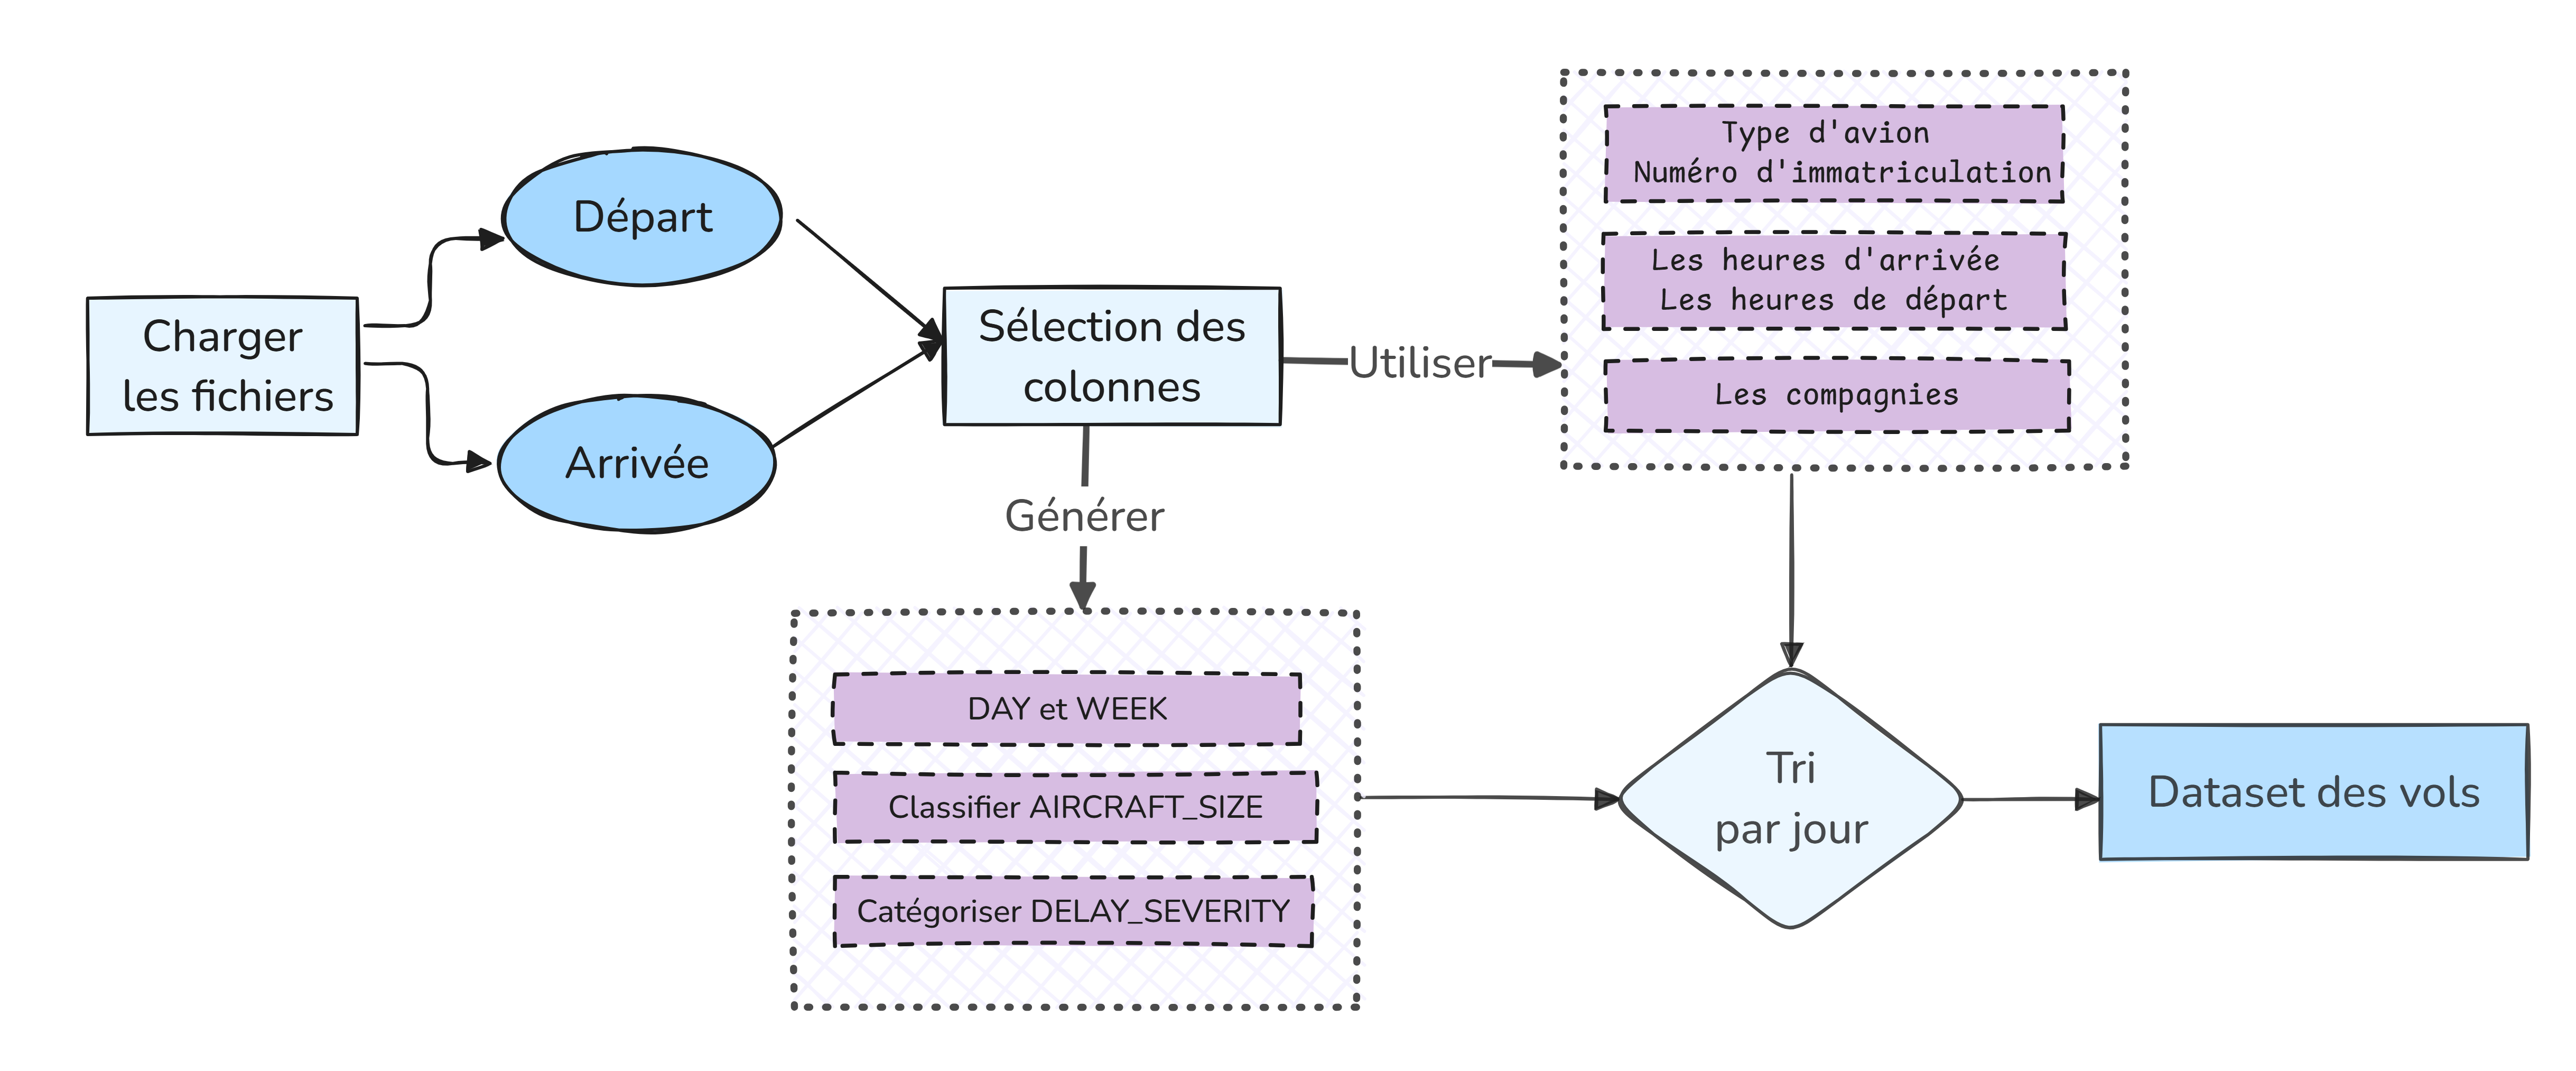
\includegraphics[width=0.9\linewidth]{assets/dataset/dataset_vol.png}
	\caption{Organigramme du processus de génération de la donnée des vols}
	\label{fig:Organigramme_vol}
\end{figure}
Le tableau suivant présente la catégorie de chaque colonne utilisée, avec le nom des colonnes, leur description et un exemple.
\begin{table}[H]
	\scriptsize
	\renewcommand{\arraystretch}{1.5}
	\caption{Jeu de données vols - Aperçu des attributs clés}
	\begin{tabularx}{\textwidth}{@{} p{3cm} p{2.7cm} X p{3.5cm} @{}}
		\toprule
		\textbf{Catégorie} & \textbf{Attribut} & \textbf{Description} & \textbf{Exemple / Type} \\
		\midrule
		
		\multirow{3}{*}{Identification du vol} & \texttt{VID} & Identifiant unique du vol & \textit{1033854621, 1033623311} \\
		\cline{2-4}
		& \texttt{FLC} & Code IATA de la compagnie aérienne & AF, LH, BA \\
		\cline{2-4}
		& \texttt{TOF} & Type de vol & Domestique, International \\
		\midrule
		
		\multirow{3}{*}{Informations avion} & \texttt{TYP} & Modèle de l’avion & A320, B737-800 \\
		\cline{2-4}
		& \texttt{REG} & Immatriculation de l’avion & FHTVS, 5CBDV \\
		\cline{2-4}
		& \texttt{SIZE} & Taille de l’avion & Petit/Moyen, Grand/Super \\
		\midrule
		
		\multirow{3}{*}{Informations temporelles} & \texttt{DAY\_DEP} & Jour du départ & Lundi, Mardi \\
		\cline{2-4}
		& \texttt{WEEK} & Numéro de semaine & 1-52 \\
		\cline{2-4}
		& \texttt{H\_DEP/H\_ARR} & Heures de départ/arrivée & 08:30, 14:15 \\
		\midrule
		
		\multirow{2}{*}{Données opérationnelles} & \texttt{SCH} & Classification zone Schengen & Oui/Non \\
		\cline{2-4}
		& \texttt{DELAY\_SEVERITY} & Classification des retards & Faible/Moyen/Élevé \\
		\bottomrule
	\end{tabularx}
	\label{tab:attributs_vols}
\end{table}




Une fois ces colonnes sélectionnées, les données ont été triées par jour. Nous avons ainsi obtenu un dataset final des vols structuré et prêt à être utilisé dans les algorithmes d’affectation.

\begin{table}[H]
	\scriptsize
	\renewcommand{\arraystretch}{0.9}
	\caption{Extrait du dataset des vols avec détails départ/arrivée et sévérité des retards}
	\begin{tabularx}{1.1\textwidth}{@{}p{1.2cm} p{1.05cm} p{1.05cm} p{0.7cm} p{0.4cm} p{0.4cm} p{0.6cm} p{0.6cm} p{0.7cm} p{0.9cm} p{0.9cm} p{0.6cm} p{1cm} p{0.6cm}@{}}
		\toprule
		\textbf{VID} & \textbf{DAY\_DEP} & \textbf{DAY\_ARR} & \textbf{WEEK} & \textbf{SCH} & \textbf{TOF} & \textbf{TYP} & \textbf{FLC} & \textbf{REG} & \textbf{SIZE} & \textbf{H\_DEP} & \textbf{D\_DEP} & \textbf{H\_ARR} & \textbf{D\_ARR} \\
		\midrule
		1033854621 & 24-11-01 & 24-11-01 & S44 & NO & I & 737 & TO & FHTVS & Medium & 08:49 & Aucun & 08:04 & Aucun \\
		
		1033623311 & 24-11-01 & 24-11-01 & S44 & NO & I & 320 & U2 & OEICJ & Medium & 09:30 & Aucun & 08:30 & Aucun \\
		
		1033654091 & 24-11-01 & 24-11-01 & S44 & Y & I & 737 & AT & CNRGF & Medium & 09:40 & Élevé & 08:36 & Aucun \\
		
		1033916281 & 24-11-01 & 24-11-01 & S44 & NO & I & 320 & U2 & OEING & Medium & 10:30 & Faible & 09:30 & Aucun \\
		
		1034969151 & 24-11-01 & 24-11-01 & S44 & NO & I & 320 & U2 & GUZHU & Medium & 14:20 & Aucun & 11:20 & Aucun \\
		
		1035003971 & 24-11-01 & 24-11-01 & S44 & NO & I & 320 & WK & HBIJV & Medium & 14:25 & Aucun & 11:30 & Moyen \\
		\bottomrule
	\end{tabularx}
	\label{tab:extrait-vols}
\end{table}




\subsection{Génération du dataset des stands}

Le processus de génération du jeu de données des \textbf{stands} repose sur une série d'étapes de traitement, de nettoyage et d’enrichissement à partir des mouvements d’aéronefs enregistrés sur la plateforme aéroportuaire. Le schéma ci-dessous illustre globalement cette chaîne de traitement.

\begin{figure}[H]
	\centering
	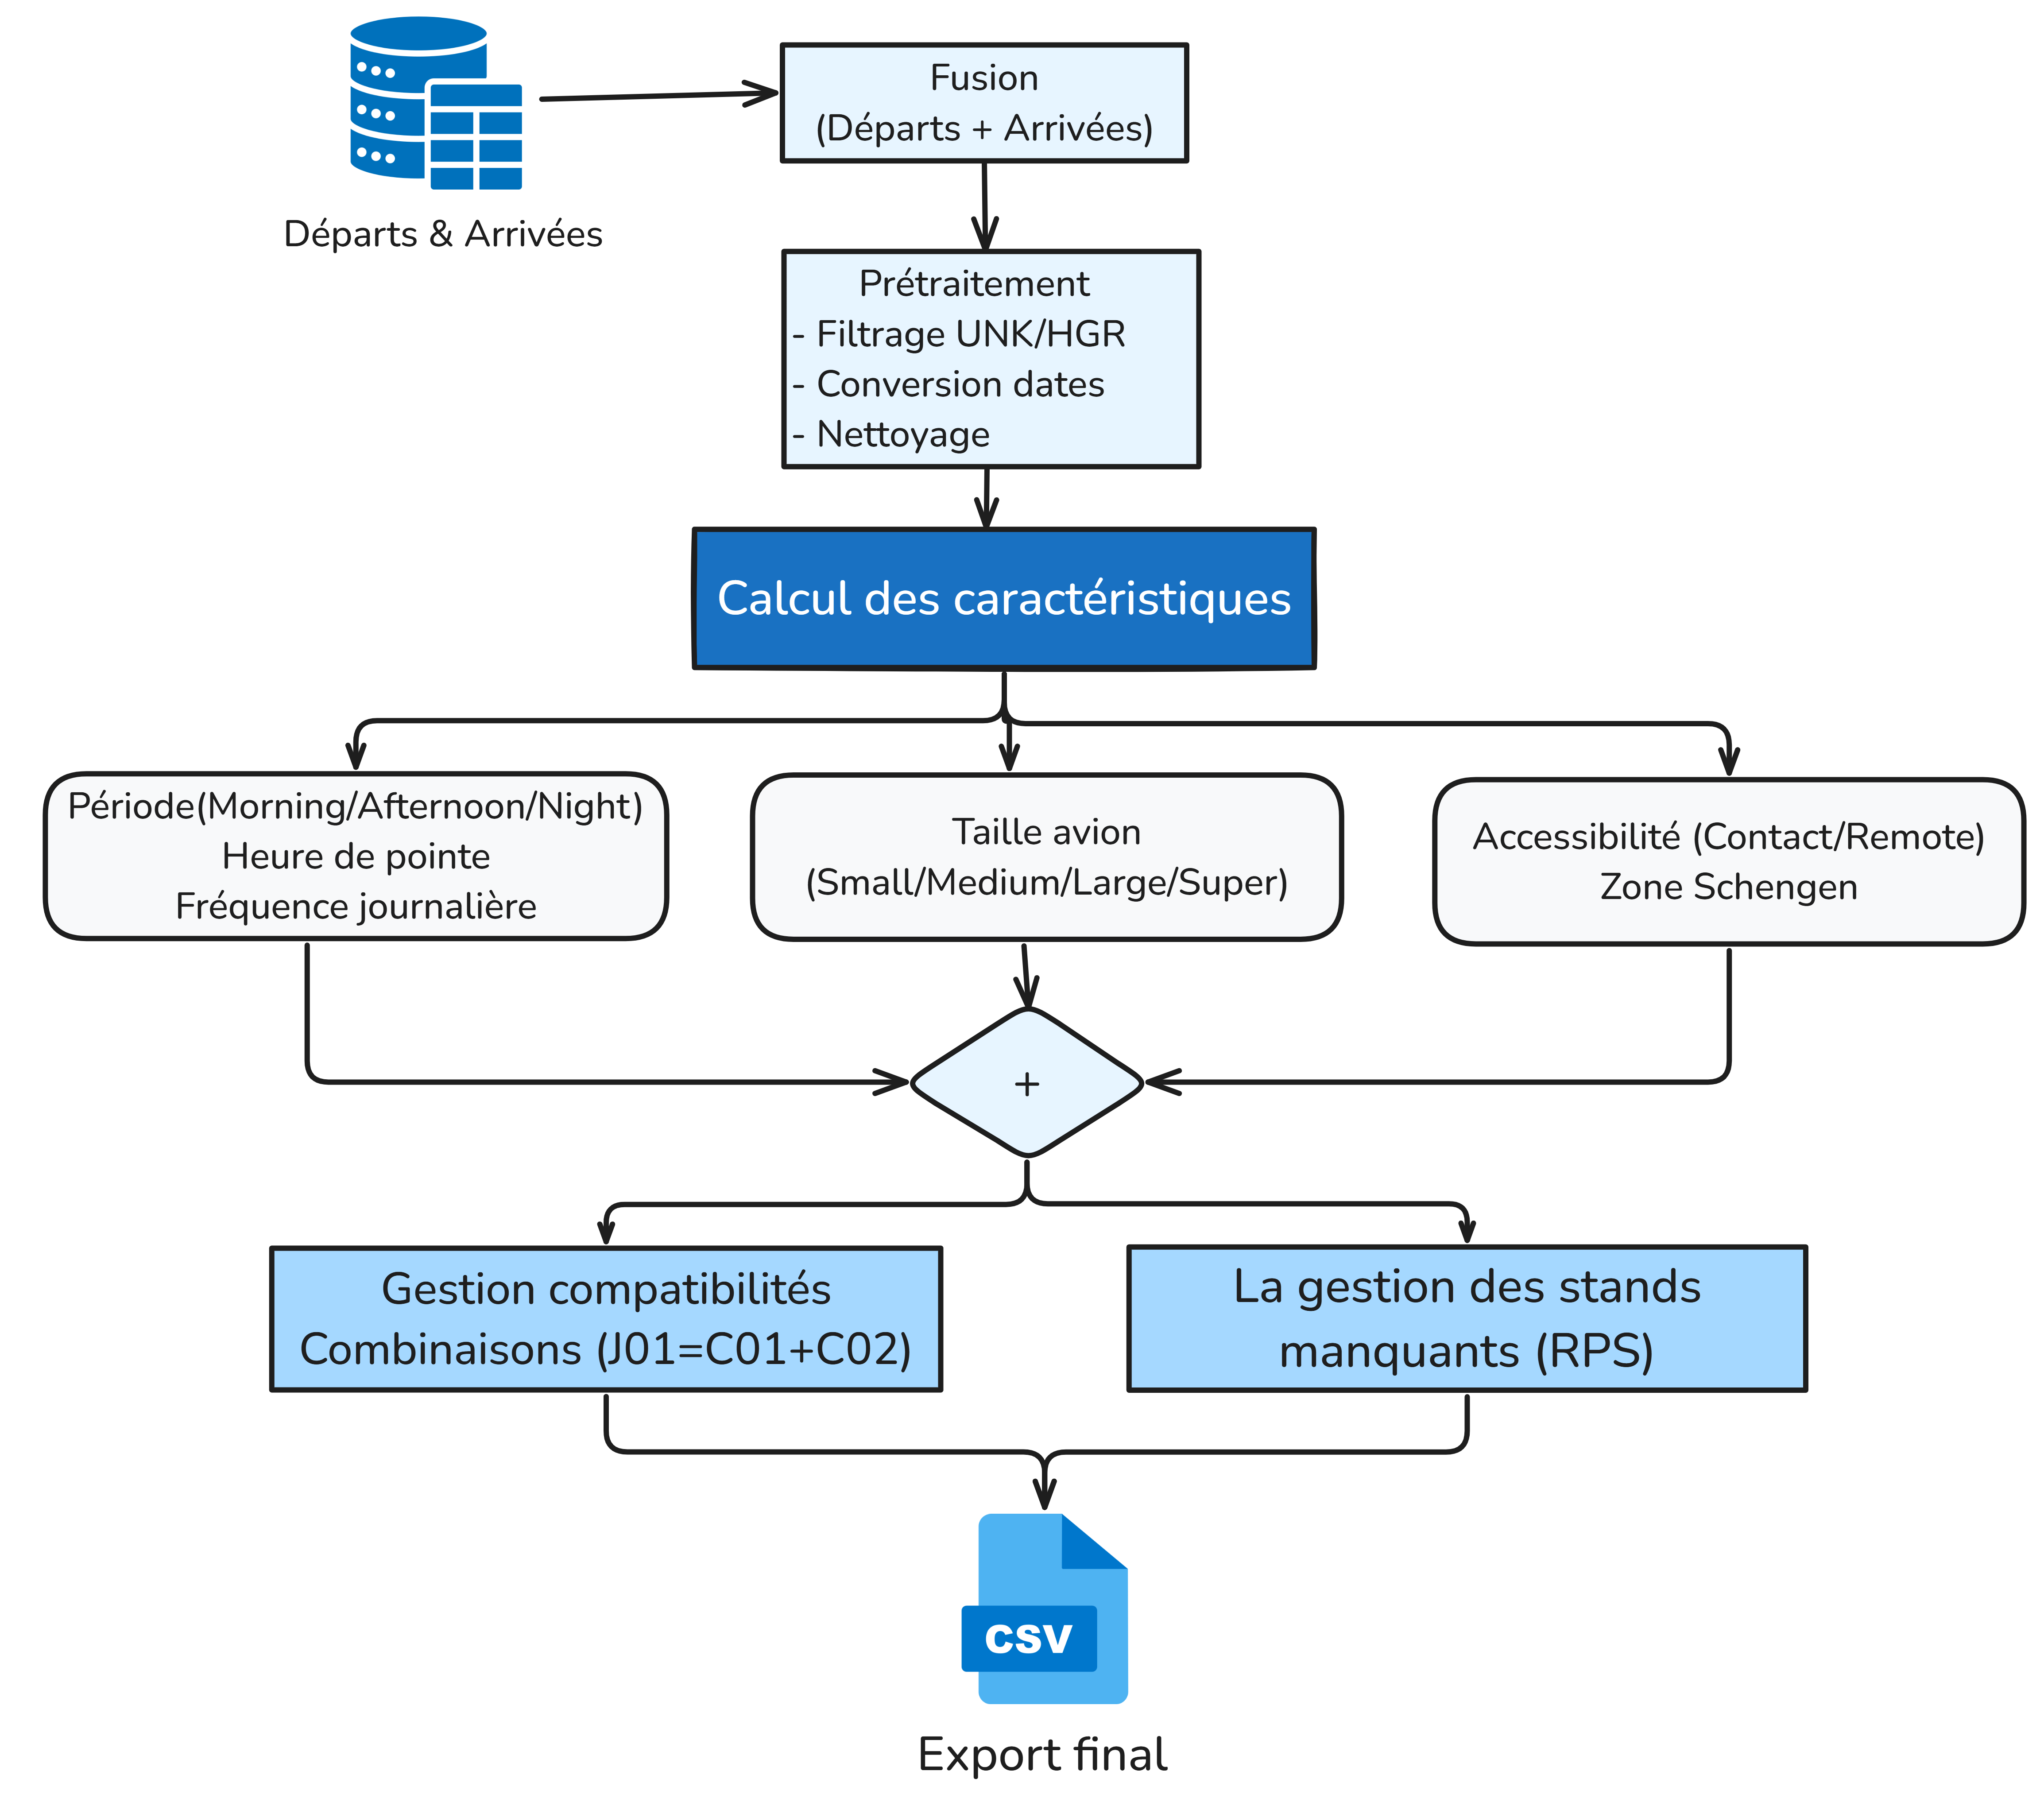
\includegraphics[width=0.6\textwidth]{assets/dataset/stand_generation.png}
	\caption{Organigramme du processus de génération de la donnée des stands}
	\label{fig:process-stands}
\end{figure}

Le traitement des données des stands s'est déroulé comme suit :

\begin{enumerate}
	\item \textbf{Collecte des données opérationnelles} à partir des historiques de mouvements d'aéronefs, en incluant :
	\begin{itemize}
		\item Le stand utilisé (\texttt{TAR}),
		\item La position de remorquage associée (\texttt{RPS}),
		\item La masse maximale au décollage (\texttt{MTW}),
		\item Le type et sous-type de l’aéronef (\texttt{TYP}, \texttt{TYS}).
	\end{itemize}
	
	\item \textbf{Nettoyage des données} :
	\begin{itemize}
		\item Suppression des enregistrements comportant des types d’aéronefs inconnus,
		\item Exclusion des aéronefs stationnés dans des hangars (\texttt{RPS = HGR}).
	\end{itemize}
	
	\item \textbf{Harmonisation et enrichissement temporel} :
	\begin{itemize}
		\item Conversion des horaires en heure locale,
		\item Déduction de la période de la journée (matin, après-midi, nuit),
		\item Identification de l’heure de pointe d’utilisation du stand (la plus fréquente),
		\item Calcul et normalisation de la fréquence maximale d’occupation journalière.
	\end{itemize}
	
	\item \textbf{Agrégation par stand} (\texttt{TAR}) afin de résumer les informations :
	\begin{itemize}
		\item Compagnies aériennes opérantes (\texttt{FLC}),
		\item Types et sous-types d'avions (\texttt{TYP}, \texttt{TYS}),
		\item Présence d’une passerelle d’embarquement (\texttt{PBB}),
		\item Statut Schengen (\texttt{SCH}).
	\end{itemize}
	
	\item \textbf{Gestion des stands non référencés} :
	\begin{itemize}
		\item Les stands uniquement présents dans \texttt{RPS} ont été considérés comme dépendants,
		\item Leurs caractéristiques ont été héritées des stands correspondants.
	\end{itemize}
	
	\item \textbf{Ajout d’une colonne de compatibilité} :
	\begin{itemize}
		\item Pour modéliser les relations fonctionnelles entre les stands,
		\item Exemple : \texttt{J01} compatible avec \texttt{C01} et \texttt{C02} (Voir Annexe \ref{fig:plan}).
	\end{itemize}
\end{enumerate}

Ce dataset consolidé fournit une base de connaissance robuste et à haute valeur ajoutée, prête à être exploitée par des algorithmes de prédiction, d’optimisation ou d’aide à la décision pour une meilleure gestion des ressources au sol dans l’environnement aéroportuaire.


\begin{table}[H]
	\centering
	\renewcommand{\arraystretch}{0.85}
	\caption{Extrait représentatif des données des stands après traitement}
	\begin{tabular}{l l l l l l l}
		\toprule
		\textbf{Stand} & \textbf{SCH} & \textbf{Fréquence} & \textbf{Heure de pointe} & \textbf{Taille Max} & \textbf{Accès} & \textbf{Compatibilité} \\
		\midrule
		B01 & YES & 21 & 10:00 PM & Medium & Contact & B01, J05, J05 \\
		\midrule
		B04 & NO  & 20 & 02:00 PM  & Medium & Contact & B04, J06, J06 \\
		\midrule
		E05 & YES & 12 & 12:00 AM  & Medium & Remote &  \\
		\midrule
		J06 & NO & 18 & 08:00 AM  & Super & Contact & J06, B03, B04 \\
		\midrule
		C23 & YES & 6 & 07:00 AM  & Super & Remote & \\
		\midrule
		B02 & NO  & 6  & 10:00 PM & Medium & Contact & B02, J05, J05 \\
		\bottomrule
	\end{tabular}
	\label{tab:extrait-stands}
\end{table}
Au total, le dataset des stands généré contient \textbf{63 lignes}, chacune représentant un stand unique, et \textbf{6 variables} principales : 
\textbf{SCH} (planification Schengen), \textbf{Fréquence} d’occupation quotidienne, \textbf{Heure de pointe}, \textbf{Taille maximale} du stand (selon la masse maximale des aéronefs accueillis), \textbf{Accès} (présence ou non de passerelle), et \textbf{Compatibilité} avec d’autres stands.
\section{Conclusion}
Dans ce chapitre, nous avons détaillé les différentes sources de données exploitées, en présentant leur structure, les variables essentielles, ainsi que les étapes de nettoyage et de préparation. L’analyse exploratoire a permis d’identifier les particularités du trafic aérien et de l’utilisation des ressources aéroportuaires.

Le chapitre suivant sera consacré à la modélisation mathématique du problème d’affectation des vols aux stands, en s’appuyant sur une revue des approches existantes, une formulation multi-objectifs et une présentation des algorithmes d’optimisation retenus.

	% \chapter{Conception fonctionnelle et technique}
\vspace{-1.5em}
\chaptertoc
\vspace{-2.5em}
\section{Introduction}

Ce chapitre décrit les étapes de la conception fonctionnelle et technique de la solution. Il couvre l’analyse des besoins, qu’ils soient fonctionnels ou non fonctionnels, l’étude de l’existant, l’architecture technique, ainsi que les technologies choisies pour le développement du système.

\vspace{-1.2em}
\section{Analyse des besoins}

Cette section identifie les besoins en distinguant les exigences fonctionnelles (comportements attendus) des non fonctionnelles (performances requises).
\vspace{-1.2em}
\subsection{Processus d’identification des besoins}
L’identification des besoins, menée par le Product Owner lors d’ateliers métier, a permis de préciser les attentes fonctionnelles, techniques et les enjeux opérationnels.

Un membre de notre équipe a assisté à une réunion sur site à l’\ac{ONDA}, facilitant l’analyse des données et les échanges avec les équipes.

Des discussions en ligne avec la DSI ont complété ce travail en clarifiant les aspects techniques et les besoins liés à l’exploitation et la qualité des données.
\vspace{-1.2em}

\subsection{Les besoins fonctionnels}

Le système doit permettre l’\textbf{ingestion, le traitement et la validation de données} issues de diverses sources (AODB, COSMOS, SMART\footnote{SMART : plateforme de supervision opérationnelle et de reporting temps réel}, SMART, Excel, API), avant leur stockage dans un datalake.

Il doit assurer une \textbf{planification intelligente des stands}, en prédisant les affectations optimales selon plusieurs critères (type d’avion, vol, occupation...), avec possibilité de comparaison à la planification actuelle (\ac{SOAM}) et d’ajustements manuels.

La solution proposera des outils de \textbf{simulation et d’aide à la décision} : simulation d’activité, visualisation via jumeau numérique et indicateurs clés (OTP, retards...).

Des \textbf{interfaces intuitives} sont attendues pour visualiser les plannings, configurer les objectifs et faciliter la coordination (chat, appels...).

Enfin, le système devra générer des \textbf{alertes personnalisables} en cas d’anomalies, et offrir une \textbf{recherche rapide} pour localiser un avion ou un stand.

\subsection{Besoins non fonctionnels}
\vspace{-0.5em}
Le système doit garantir la \textbf{sécurité et la gouvernance des données} (authentification, autorisation, chiffrement, traçabilité et gestion du cycle de vie).

Il doit être \textbf{scalable et compatible avec le Cloud}, via une architecture modulaire et une intégration avec des plateformes comme Cloudera.

La \textbf{surveillance et l’automatisation} sont également clés : supervision proactive des flux critiques et automatisation des services sensibles.

L’\textbf{interopérabilité} avec les systèmes \ac{ONDA} existants est requise, assurant des échanges fluides entre Cloudera et les bases métier.

Enfin, la \textbf{gestion des risques} implique l’identification des menaces potentielles et la mise en œuvre de plans de contingence adaptés.

\vspace{-1.2em}

\section{Analyse de l’existant}

Avant de proposer une solution d’optimisation, il est essentiel d’analyser l’existant afin d’identifier les forces et les limites du système actuellement en place.
\vspace{-1.2em}
\subsection{Étude de l'existant}

\noindent
Le Système d'Optimisation et d'Affectation des Moyens (\ac{SOAM}) s’inscrit dans la feuille de route 2018–2025 de modernisation de l’\ac{ONDA}. Il a pour vocation de centraliser et automatiser la planification des ressources aéroportuaires dans 22 aéroports marocains.  

\vspace{0.6em}  

\textbf{Planification saisonnière.} Les compagnies aériennes transmettent leurs plannings (été/hiver) au coordinateur marocain des créneaux horaires aériens (MSC)\footnote{MSC : \textit{Moroccan Slot Coordinator}} sous format Excel. Ces fichiers sont ensuite transférés manuellement à la cellule de planification des vols (CPV)\footnote{CPV : Cellule de Planification des Vols}.  

\vspace{0.6em}  

\textbf{Intégration dans SOAM.} Les données sont vérifiées et converties manuellement au format CSV. Le chargement dans le système doit être fait cinq jours avant le début de la saison. Aucun mécanisme de validation automatique n’est mis en place, exposant à des erreurs de saisie.   

\vspace{0.6em}  

\textbf{Gestion des modifications.} Les mises à jour des vols (horaires, annulations...) sont reçues soit via \textbf{SITA} (intégration automatique), soit via \textbf{Outlook} (traitement manuel par la cellule PCO\footnote{PCO : \textit{Poste de Coordination Opérationnelle}}).  

\vspace{0.6em}  

\textbf{Visualisation des stands.} Une interface graphique (Figure~\ref{fig:graphiqueSOAM}) permet de visualiser les avions affectés aux stands sur le plan de l’aéroport. Cette vue facilite la coordination opérationnelle en montrant la position physique des aéronefs, les zones de sécurité, et les services de piste.

\begin{figure}[H]
	\centering
	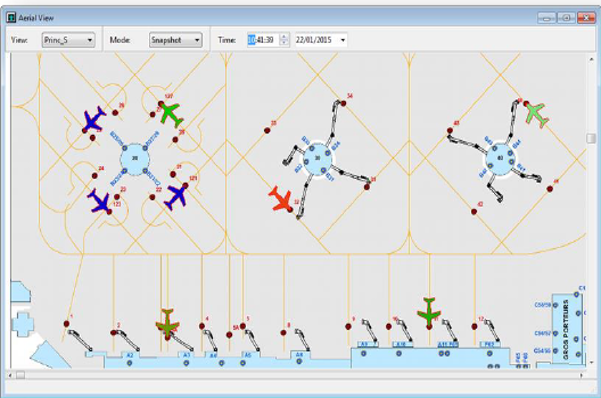
\includegraphics[width=0.5\textwidth]{assets/diagrams/graphiqueSOAM.png}
	\caption{Vue graphique de la planification des stands sur le plan de l'aéroport}
	\label{fig:graphiqueSOAM}
\end{figure}
\vspace{-1.2em}
\textbf{Mécanisme de planification.} \ac{SOAM} repose sur un ensemble de règles prédéfinies pour générer une planification initiale, qui peut être manuellement ajustée en cas de conflit. Aucune logique d’optimisation ni moteur d’aide à la décision n’est actuellement intégré.

\subsection{Identification des limitations de l'existant }

Le système actuel présente quatre principales limites :  

\begin{enumerate}
	\item \textbf{Processus inefficaces} : forte dépendance aux interventions manuelles, avec des délais importants entre réception et intégration des plannings.  
	\item \textbf{Manque d’intelligence} : absence d’IA, sans recommandations ni simulations, fonctionnement basé sur des règles statiques sans adaptation dynamique.  
	\item \textbf{Fonctionnalités limitées} : interfaces peu ergonomiques, pas de visualisation 3D ni collaboration intégrée, absence d’indicateurs avancés (KPI).  
	\item \textbf{Impact sur la performance} : sous-utilisation des ressources, mauvaise gestion des crises, expérience utilisateur dégradée (lenteur, difficulté d’apprentissage).
\end{enumerate}

En résumé, le \ac{SOAM} répond aux besoins de base, mais reste limité en résilience et optimisation. Une plateforme intelligente, modulaire, connectée, intégrant un \textit{data lake}, l’IA et un jumeau numérique, s’impose.


\vspace{-1.2em}




\section{Architecture technique}

Cette section présente la structure technique sur laquelle repose la solution proposée, en mettant en avant ses composants clés et l'architecture d'intelligence artificielle

\subsection{Vue d'ensemble}

La modernisation des opérations aéroportuaires vise plusieurs objectifs interdépendants : optimiser les flux passagers, améliorer la gestion des bagages, coordonner les rotations avion, anticiper les capacités et planifier intelligemment les stands. Ces fonctions nécessitent une infrastructure unifiée capable de traiter des données hétérogènes en temps quasi réel.

La planification des stands joue un rôle central dans cette chaîne. Elle impacte directement la ponctualité, l’occupation des ressources au sol et la fluidité globale des opérations. La solution proposée s’appuie sur une architecture modulaire et scalable, intégrant les technologies Big Data et l’IA pour analyser les données issues de multiples sources (\ac{AODB}, météo, mouvements avion...).


\begin{figure}[H]
	\centering
	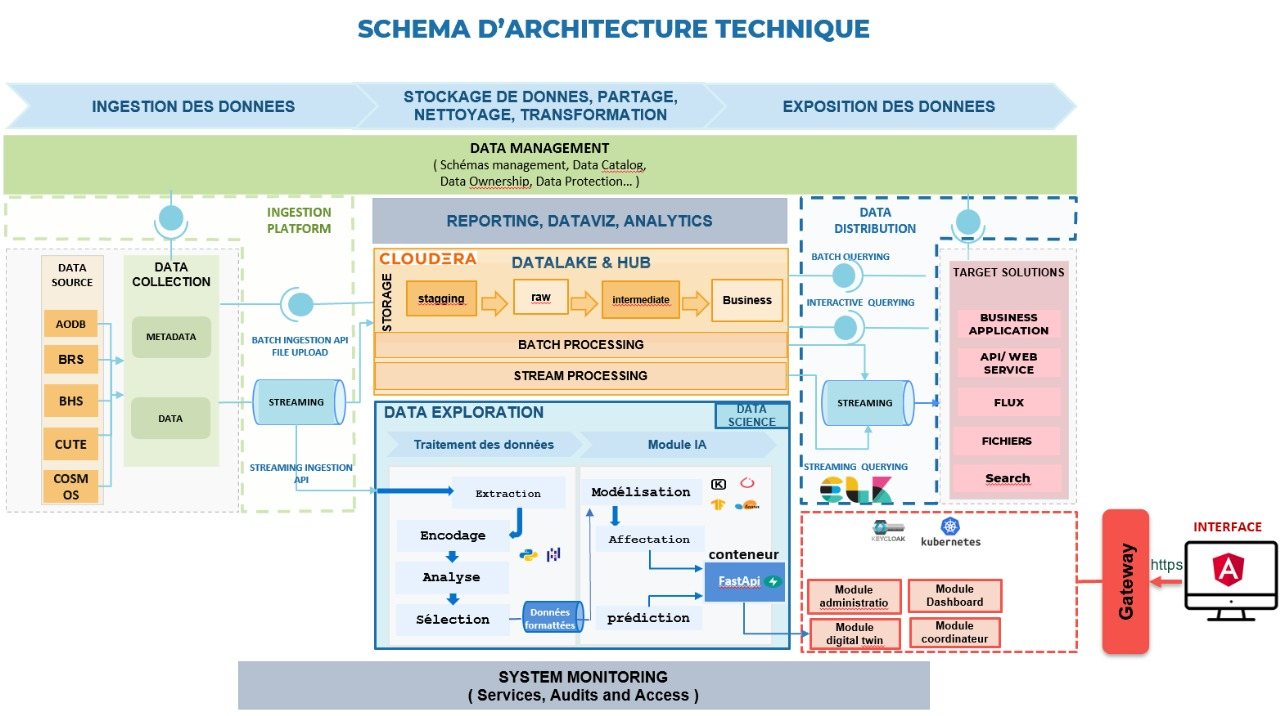
\includegraphics[width=1.1\linewidth]{assets/architecture/architecture.jpg}
	\caption{Architecture globale de la solution intelligente de la planification des stands}
	\label{fig:architecture}
\end{figure}

L’architecture se compose des éléments suivants :

\begin{itemize}
	\item \textbf{Sources de données} : les données sont collectées en temps quasi réel à partir de systèmes existants comme \ac{AODB}, COSMOS\footnote{COSMOS : système de gestion technique et logistique des infrastructures aéroportuaires}, fichiers Excel, API et autres bases relationnelles.
	
	
	\item \textbf{Ingestion et traitement des données} : un pipeline d’ingestion automatisé alimente un \textbf{Data Lake} hébergé sur une plateforme Big Data \textbf{(Cloudera)}, en assurant le nettoyage, la normalisation et la transformation des données.
	
	\item \textbf{Stockage centralisé} : les données sont stockées de manière structurée et non structurée dans le Data Lake, facilitant les accès parallèles et les traitements distribués.
	
	\item \textbf{Moteur d’intelligence artificielle} : les modèles d’optimisation (basés sur le Machine Learning et des algorithmes de recherche opérationnelle) utilisent les données historiques et en temps quasi réel pour générer des recommandations de planification.
	
	\item \textbf{Moteur de simulation} : permet de tester plusieurs scénarios de planification (ex : jour perturbé, saturation, retards massifs) et d’évaluer les impacts sur la performance.
	
	\item \textbf{Interface utilisateur} : une application graphique (vue 3D) permet aux équipes opérationnelles de consulter les recommandations, visualiser les affectations sur un plan de l’aéroport, simuler des scénarios, et interagir avec le système (modification, validation, alertes, chat).
	
	\item \textbf{Reporting et pilotage} : des tableaux de bord fournissent des indicateurs clés (KPI) tels que le taux d’occupation, l’OTP (on-time performance), le taux de replanification, ou encore les conflits évités.
\end{itemize}




Cette architecture répond aux besoins de performance, de flexibilité et d’adaptabilité d’un environnement aéroportuaire en constante évolution.



\subsection{Zoom sur l'architecture du module d’intelligence artificielle}


Le module d’intelligence artificielle constitue le cœur du système d’optimisation. Il est conçu pour automatiser et améliorer les décisions relatives à l’affectation des stands, tout en offrant une extensibilité vers d’autres cas d’usage futurs (flux passagers, rotations, bagages, capacités, etc.).

\begin{figure}[H]
	\centering
	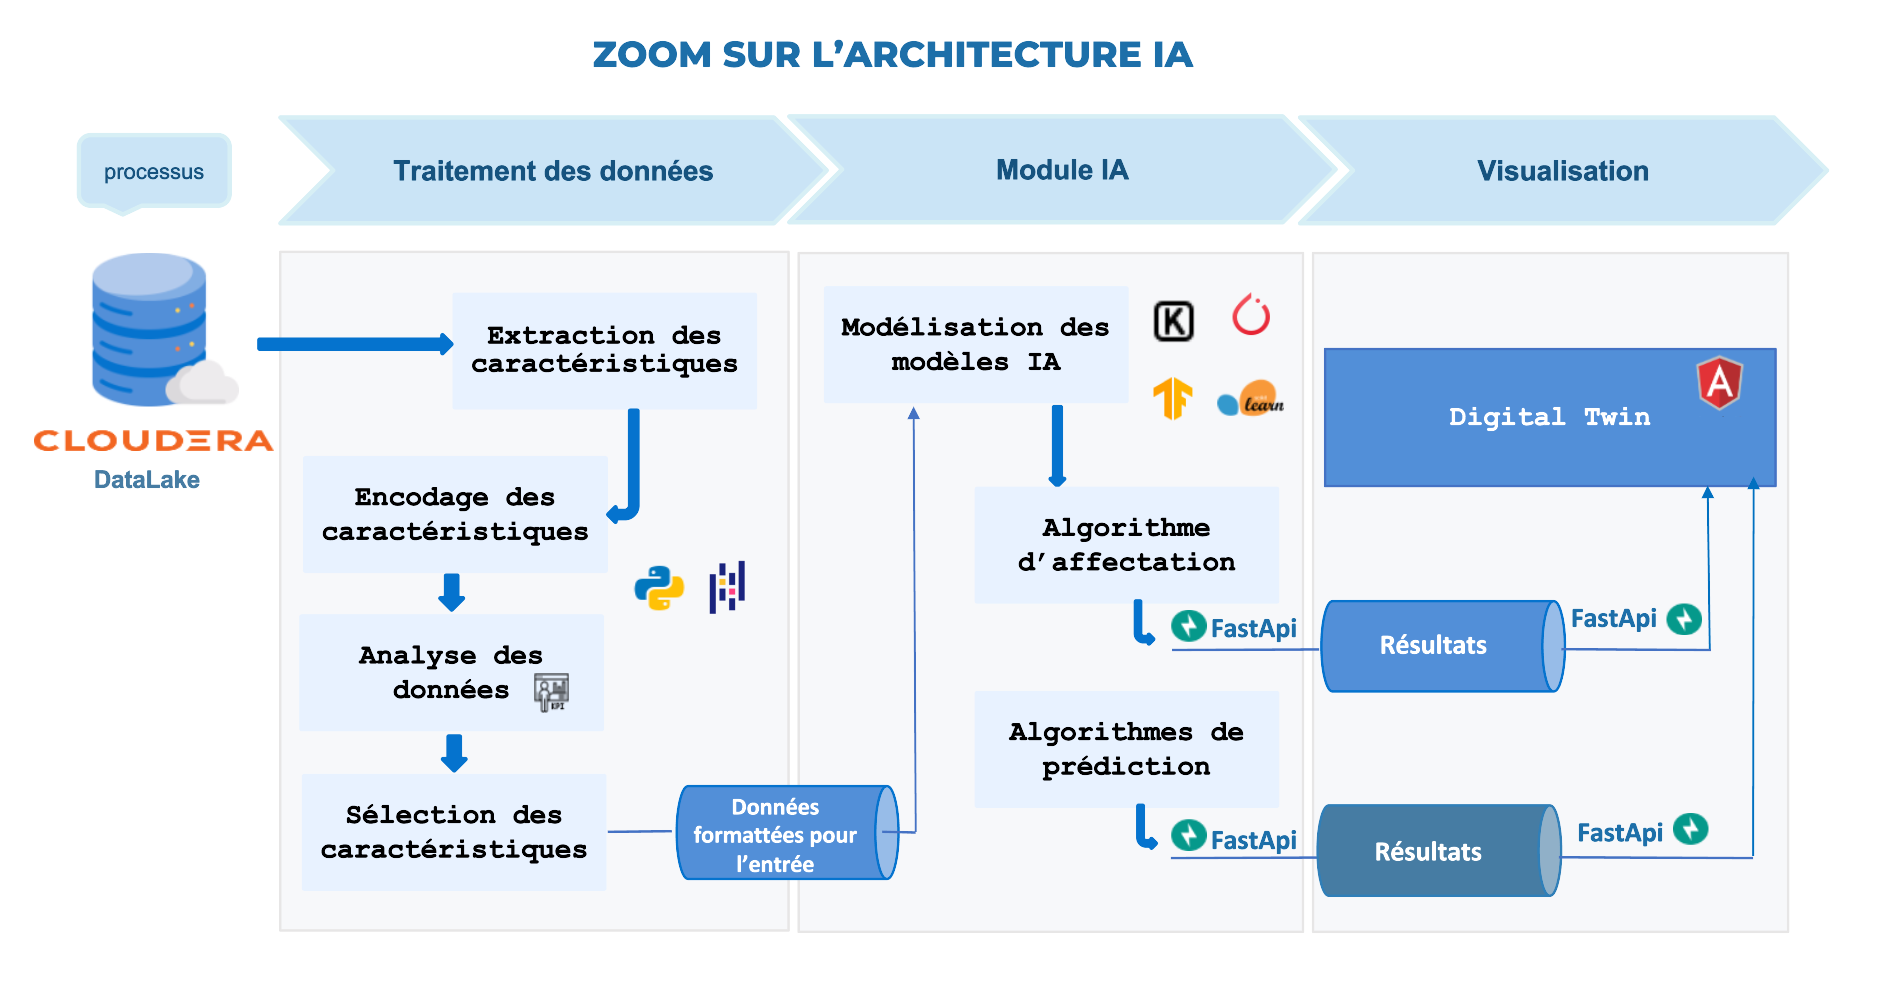
\includegraphics[width=1.1\linewidth]{assets/architecture/moduleIA.png}
	\caption{Pipeline du module IA}
	\label{fig:moduleIA}
\end{figure}


L’architecture \ref{fig:moduleIA} de ce module suit un pipeline structuré en plusieurs phases :

\begin{enumerate}
	\item \textbf{Prétraitement et préparation des données} \\[0.3em]
	Cette première étape consiste à transformer les données brutes collectées depuis les différentes sources en un format exploitable pour l’apprentissage et l’optimisation. Elle inclut :
	\begin{itemize}
		\item \textbf{Extraction des caractéristiques} : identification des variables pertinentes comme le type d’aéronef, la durée d’escale, les contraintes de compatibilité avec les stands.
		\item \textbf{Encodage des caractéristiques} : transformation des variables catégorielles (ex. type d’avion, terminal) en formats numériques utilisables par les modèles d’apprentissage.
		\item \textbf{Analyse exploratoire des données} : identification d’anomalies, visualisation des distributions, corrélations entre variables, et détection de valeurs manquantes.
		\item \textbf{Sélection des caractéristiques} : réduction de la dimensionnalité via des méthodes statistiques ou algorithmiques pour conserver les variables les plus influentes.
	\end{itemize}
	
	\item \textbf{Modélisation et optimisation IA} \\[0.3em]
	Les données préparées sont injectées dans des modèles IA en fonction du cas d’usage :
	\begin{itemize}
		\item \textbf{Algorithmes d’affectation et d’optimisation} : utilisés pour générer un planning optimisé des stands selon des contraintes d’exploitation et de compatibilité.
		\item \textbf{Modèles de prédiction et Deep Learning} : prévus pour les objectifs futurs tels que la prévision de flux passagers, la détection de saturation, ou l’anticipation de conflits.
	\end{itemize}
	
	\item \textbf{Déploiement via API et conteneurisation} \\[0.3em]
	Une fois le planning optimisé généré, les résultats sont encapsulés dans une API REST, développée avec \textbf{FastAPI}. Cette API est conteneurisée à l’aide de \textbf{Docker}.
	
	\item \textbf{Intégration applicative et visualisation} \\[0.3em]
	L’image Docker produite est transmise à l’équipe de développement pour intégration dans la plateforme. Cela permet :
	\begin{itemize}
		\item d’alimenter le \textbf{jumeau numérique} avec des scénarios réalistes de planification,
		\item d’exploiter les recommandations IA dans l’interface utilisateur,
		\item de suivre les impacts des décisions sur les KPI définis, avec traçabilité des ajustements.
	\end{itemize}
\end{enumerate}

%La figure suivante illustre l’ensemble de ce pipeline technique, de la collecte initiale des données jusqu’à l’intégration des résultats dans l’environnement applicatif.



\section{Environnements logiciels et technologies}

Cette section présente les outils, langages et environnements utilisés au cours du projet, en justifiant les choix technologiques réalisés à chaque étape.Une veille technologique a également été menée dans le cadre de l'exploration des solutions open-source pour le Digital Twin.

\subsection{Technologies utilisées}

Afin de mettre en œuvre le projet selon l’architecture définie, nous avons mobilisé plusieurs technologies :

\vspace{0.3cm}

\noindent\textbf{Python} — Langage principal utilisé pour le développement des algorithmes d’optimisation et les traitements de données. Python a été choisi pour sa flexibilité, sa lisibilité, ainsi que la richesse de son écosystème. Les bibliothèques suivantes ont été mobilisées :
\begin{itemize}
	\item \texttt{Pandas}, \texttt{NumPy} : manipulation et analyse de données ;
	\item \texttt{scipy.optimize}, \texttt{PuLP} : modélisation et résolution de problèmes d’optimisation ;
	\item \texttt{datetime} : gestion des dates/heures ;
	\item \texttt{matplotlib} et \texttt{Plotly} : visualisation des résultats.
\end{itemize}

\begin{figure}[H]
	\centering
	
\includegraphics[width=0.2\linewidth]{assets/logos/python.png}
	\label{fig:logo-python}
\end{figure}

\vspace{0.2cm}

\noindent\textbf{Plotly} — Utilisé pour la visualisation interactive des résultats. Contrairement à \texttt{Matplotlib}, \texttt{Plotly} permet d'explorer dynamiquement les données (zoom, survol, filtrage) et d’inspecter les distributions colonne par colonne.

\begin{figure}[H]
	\centering
	
\includegraphics[width=0.3\linewidth]{assets/logos/plotly.png}
	\label{fig:logo-plotly}
\end{figure}


\noindent\textbf{Visual Studio Code (VS Code)} — IDE principal utilisé pour le développement. Il propose :
\begin{itemize}
	\item des extensions Python avec débogage avancé ;
	\item un terminal intégré facilitant les tests et le déploiement ;
	\item l’auto-complétion intelligente (IntelliSense).
\end{itemize}
Ces fonctionnalités améliorent considérablement la productivité et permettent une configuration adaptée grâce aux extensions communautaires.

\begin{figure}[H]
	\centering
	
\includegraphics[width=0.1\linewidth]{assets/logos/vsCode.png}

	\label{fig:logo-vscode}
\end{figure}

\vspace{0.2cm}

\noindent\textbf{FastAPI} — Framework Python utilisé pour la création d’API RESTful, facilitant le test des services backend.

\begin{figure}[H]
	\centering
	
\includegraphics[width=0.2\linewidth]{assets/logos/fastApi.png}
	\label{fig:logo-fastapi}
\end{figure}

\vspace{0.2cm}

\noindent\textbf{Docker} — Il simplifie la création, le partage, le test et le déploiement des applications en les emballant dans des conteneurs.

\begin{figure}[H]
	\centering
	
\includegraphics[width=0.2\linewidth]{assets/logos/docker.png}
	\label{fig:logo-docker}
\end{figure}

\vspace{0.2cm}

\noindent\textbf{Bitbucket} — Plateforme de gestion de version basée sur Git, utilisée pour le suivi des modifications du code source, la collaboration entre développeurs.

\begin{figure}[H]
	\centering
	
\includegraphics[width=0.25\linewidth]{assets/logos/bitbucket.png}
	\label{fig:logo-github}
\end{figure}






\subsection{Technologies utilisées par l’équipe de développement}

\begin{itemize}
	\item \textbf{Angular} : framework utilisé pour le développement de l’interface utilisateur. Bien qu’il n’ait pas été directement manipulé, il constitue la base du front-end de la solution finale.
	\begin{figure}[H]
		\centering
		
\includegraphics[width=0.2\linewidth]{assets/logos/angular.png}
		\label{fig:scrum}
	\end{figure}
	
	\item \textbf{Three.js} : bibliothèque JavaScript utilisée pour la visualisation 3D du Digital Twin, notamment la représentation des avions et des stands dans un environnement interactif.
	\begin{figure}[H]
		\centering
		
\includegraphics[width=0.25\linewidth]{assets/logos/threeJs.png}
		\label{fig:scrum}
	\end{figure}
\end{itemize}

\subsection{Veille technologique sur les outils de Digital Twin}

Dans le cadre de l’exploration des technologies open-source pour la simulation des opérations aéroportuaires, une veille technologique a été menée, alors plusieurs technologies ont été explorées lors de cette phase, notamment :
\begin{itemize}
	\item \textbf{AnyLogic} : puissant mais propriétaire, avec une courbe d’apprentissage importante.
	\item \textbf{Unity + C\#} : très flexible pour la 3D, mais peu adapté à une intégration web simple.
	\item \textbf{CesiumJS} : excellent pour la visualisation géospatiale, mais moins orienté opérationnels.
	\item \textbf{Babylon.js} : alternative à Three.js avec de bonnes performances graphiques.
\end{itemize}  
\vspace{0.3cm}

À l’issue de cette veille, la plateforme \textbf{GAMA} a été retenue pour les premiers prototypes. 
\begin{itemize}
	\item \textbf{GAMA} : plateforme open-source puissante pour la modélisation multi-agents, utilisée initialement pour deux scénarios de simulation de gestion de stands. 
	\begin{figure}[H]
		\centering
		
\includegraphics[width=0.13\linewidth]{assets/logos/gama.png}
		\label{fig:scrum}
	\end{figure}
	Deux scénarios de simulation ont ainsi été développés. Toutefois, ses limitations en matière d’intégration avec des interfaces front-end web ont conduit à un réajustement technologique.
	
\end{itemize}

\subsection{Comparaison des outils de Digital Twin}

Le tableau~\ref{tab:comparaison_dt} présente une comparaison synthétique entre deux outils envisagés pour le développement du jumeau numérique : \textbf{GAMA} et \textbf{Three.js + Angular}.

\begin{table}[H]
	\centering
	\renewcommand{\arraystretch}{1.1}
	\caption{Comparaison entre GAMA et Three.js + Angular}
	\begin{tabular}{lll}
		\toprule
		\textbf{Critère} & \textbf{GAMA} & \textbf{Three.js + Angular} \\
		\midrule
		Nature & Modélisation multi-agents & Visualisation 3D web interactive \\
		Courbe d’apprentissage & Modérée à élevée & Moyenne (si base en JS/TS) \\
		Intégration front-end & Limitée & Excellente \\
		Interopérabilité avec API & Faible & Haute (via services REST) \\
		Personnalisation graphique & Basique & Avancée (textures, caméras, lumière) \\
		Conclusion & Bon pour les prototypes & Choisi pour le rendu final \\
		\bottomrule
	\end{tabular}
	\label{tab:comparaison_dt}
\end{table}

La combinaison \textbf{Three.js + Angular} a finalement été retenue pour sa capacité à offrir une visualisation 3D web interactive, fluide, et facilement intégrable dans l’interface utilisateur du système final.


\vspace{0.5cm}


\section{Conclusion}
Ce chapitre a présenté la conception fonctionnelle et technique de notre solution, en partant de l’analyse des besoins jusqu’au choix des technologies. Nous avons détaillé l’architecture globale du système ainsi que celle du module d’intelligence artificielle. Une étude comparative des outils de Digital Twin a également permis de justifier les choix technologiques retenus.

Le chapitre suivant portera sur les données utilisées dans notre projet, en décrivant leur source, leur structure, ainsi que les étapes d’analyse et de préparation nécessaires à l'entraînement du modèle.
	% \chapter{Modélisation Mathématique}
\vspace{-1.5em}
\chaptertoc
\vspace{-2.5em}
\vspace{-0.3cm}
\section{Introduction}
Ce chapitre débute par une revue de littérature présentant les principales approches d'affectation des stands proposées dans les travaux antérieurs. Il introduit ensuite la modélisation du problème, en détaillant les contraintes identifiées, les algorithmes d'affectation retenus, ainsi que les hyperparamètres associés. Enfin, les métriques utilisées pour l’évaluation des performances.
\vspace{-0.5cm}
\section{Revue de littérature}
\label{sec:classical}
\vspace{-0.5em}
Dans cette section, nous présentons une revue des approches existantes permettant de résoudre le problème d’affectation des avions aux stands.

\vspace{-1em}
\subsection{Définition du problème}

L’\ac{SAP} joue un rôle essentiel dans la gestion aéroportuaire. Son objectif est d’attribuer à chaque avion une position au sol pour les opérations de débarquement, embarquement, maintenance et ravitaillement. Une allocation optimale améliore la fluidité des opérations, maximise l’utilisation des infrastructures et réduit les coûts, tout en garantissant la ponctualité des vols et le confort des passagers \cite{Das_2020}.
\vspace{-2.5em}
\begin{figure}[H]
	\centering
	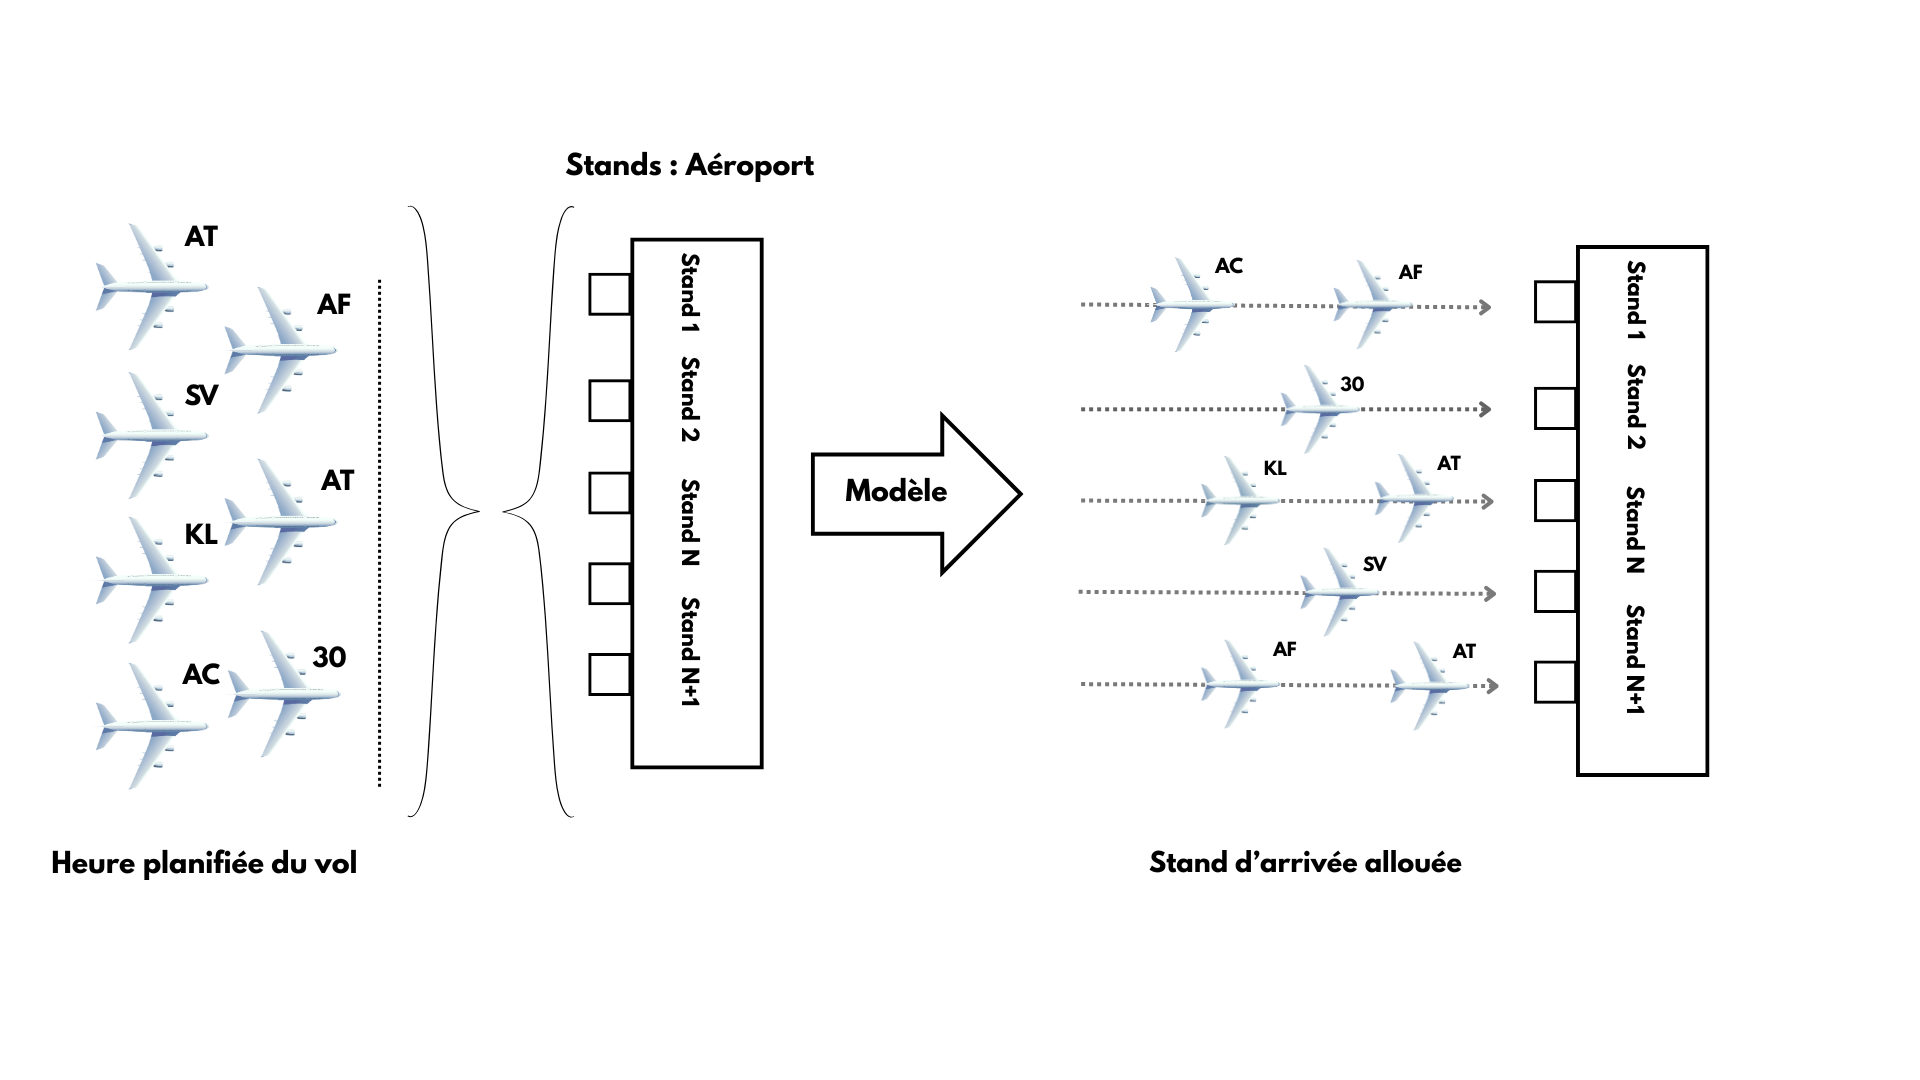
\includegraphics[width=0.7\linewidth]{assets/dataset/probleme.png}
	\caption{Définition du problème SAP}
	\label{fig:SAP}
\end{figure}
\vspace{-1.5em}
La figure \ref{fig:SAP} illustre le principe général de l’\ac{SAP}.  
Cependant, la résolution de l’\ac{SAP} représente un défi complexe en raison des multiples contraintes à prendre en compte : compatibilité avion/stand, contraintes temporelles, connexions entre vols et imprévus (tels que les retards). Ce problème, classé NP-difficile, devient rapidement ingérable par des méthodes exactes dans les grands aéroports, où des milliers de vols quotidiens — parfois plus de 300 par jour — doivent être répartis sur des dizaines de stands, générant un nombre astronomique de combinaisons possibles \cite{NilBusquetsTrias}.

Pour faire face à cette complexité, plusieurs approches d’optimisation ont été proposées et peuvent être regroupées en trois grandes catégories :
\begin{itemize}
	\item \textbf{Méthodes exactes}, qui garantissent une solution optimale sans violation des contraintes, mais sont limitées à des instances de petite taille et à des algorithmes spécialisés comme l’\textbf{algorithme hongrois} pour les problèmes d’affectation.
	\item \textbf{Heuristiques}, qui permettent d’obtenir des solutions approximatives rapidement.
	\item \textbf{Métaheuristiques}, qui explorent efficacement l’espace de recherche afin d’obtenir des résultats de haute qualité en un temps raisonnable.
\end{itemize}

Ces méthodes s’appliquent aussi bien à des contextes statiques, avec une planification préétablie, qu’à des contextes dynamiques nécessitant des ajustements en temps réel face aux imprévus et aux changements de dernière minute \cite{Cheng_2012}.

\subsection{Approches existantes}

Cette partie présente plusieurs approches d’optimisation qui ont été proposées.

\subsection*{Méthodes exactes}
\vspace{-0.5em}
Les méthodes exactes s’appuient sur une modélisation mathématique rigoureuse du problème d’\ac{SAP}, permettant de garantir l’optimalité des solutions pour des instances de taille raisonnable. Elles reposent principalement sur la \textbf{\ac{PL}}, \textbf{l'optimisation linéaire en nombres entiers} et les algorithmes de type \textbf{branch-and-bound} \cite{Bolat_2001,Li_2021}.
\vspace{-0.5em}
\subsubsection*{\small{\textcolor{blue}{Programmation Linéaire (PL/PLNE)}}}

\label{sec:LP}


L’\ac{SAP} est souvent modélisé comme un problème d’optimisation (linéaire ou mixte) visant à minimiser un coût (préférences, attente, déplacements). Il offre des résultats précis en temps raisonnable pour des cas moyens, mais peut exiger des ajustements manuels.

\textbf{Principe général :} La \ac{PL} optimise une fonction objectif linéaire sous des contraintes d’égalité et d’inégalité. Elle constitue la base de nombreux problèmes d’optimisation et se résout efficacement avec des algorithmes comme le simplexe. \textit{La solution optimale se trouve à un sommet de la région réalisable définie par les contraintes.}
\begin{algorithm}[H]
	\caption{Méthode du Simplexe pour la Programmation Linéaire}
	\label{alg:simplex}
	\begin{algorithmic}[1]
		\Require Coefficients de la fonction objectif $c$, matrice de contraintes $A$, bornes $b$
		\Ensure Solution optimale $x^*$ et valeur optimale $z^*$
		
		\State Convertir le problème en forme standard avec variables d'écart
		\State Initialiser une solution de base réalisable
		
		\Repeat
		\State Calculer les coûts réduits $c_j - c_B^T A_j$ pour toutes les variables non basiques
		\If{tous les coûts réduits $\geq 0$}
		\State \Return solution courante comme optimale
		\EndIf
		\State Sélectionner la variable entrante $x_k$ avec le coût réduit le plus négatif
		\State Calculer le vecteur direction $d = B^{-1} A_k$
		\If{$d \leq 0$}
		\State \Return le problème est non borné
		\EndIf
		\State Déterminer la variable sortante par le test du ratio minimal
		\State Mettre à jour la base et la solution
		\Until{convergence atteinte}
	\end{algorithmic}
\end{algorithm}
\vspace{-0.5em}
\textbf{Applications de recherche dans le SAP :}  
Pour dépasser les limites des modèles classiques, plusieurs auteurs ont introduit des extensions stochastiques afin de mieux gérer l’incertitude. Lim et al. \cite{Lim_2005} ont développé un modèle en deux étapes utilisant une distribution discrète pour représenter l’incertitude sur l’heure d’arrivée, basé sur la décomposition de Benders\footnote{La décomposition de Benders divise un problème en un problème maître et des sous-problèmes, facilitant sa résolution.}.

Dans une approche dynamique, Li et al. \cite{Li_2021} ont proposé un modèle multi-étapes basé sur des arbres de scénarios, intégrant décomposition hiérarchique et gestion du risque. Trias Busquets \cite{NilBusquetsTrias} a, de son côté, couplé \ac{PL} et \ac{GA} pour planifier l’affectation des stands.

\vspace{-0.5em}
\subsubsection*{\small{\textcolor{blue}{Méthodes Branch-and-Bound}}}


Les méthodes branch-and-bound explorent systématiquement l’espace des solutions en éliminant celles non optimales à l’aide de fonctions de bornes. Bien qu’elles garantissent l’optimalité, leur coût de calcul devient élevé pour les grandes instances.

\textbf{Principe général :}  
Partitionner systématiquement l’espace des solutions en sous-problèmes plus petits (ramification) et utiliser des bornes pour écarter ceux qui ne peuvent pas contenir la solution optimale, réduisant ainsi l’espace de recherche sans perdre la garantie d’optimalité.
\textbf{Applications de recherche dans le SAP :}  
Qin et al. \cite{Qin_2012} ont proposé une approche \textit{branch-and-price} exploitant la structure du problème via la génération de colonnes pour améliorer l’efficacité.


Guépet et al. \cite{Guepet_2016} ont développé un algorithme de \textit{branch-and-bound} enrichi par des coupes valides spécifiques à l’\ac{SAP}, intégrant également une phase de prétraitement permettant d’éliminer en amont les affectations incompatibles, réduisant ainsi l’espace de recherche.
\vspace{-0.5em}
\subsubsection*{\small{\textcolor{blue}{Algorithme Hongrois}}}
\label{sec:Hungarian}

\vspace{-0.5em}
L’algorithme hongrois est une méthode d’optimisation combinatoire spécialement conçue pour les problèmes d’affectation. Il constitue une approche spécialisée pour résoudre les problèmes de \ac{PL} carrée, dans lesquels le nombre d’agents et de tâches est égal.

\textbf{Principe général :}  
L’algorithme hongrois repose sur le fait que l’ajout ou le retrait d’une constante à une ligne ou une colonne de la matrice des coûts ne change pas l’affectation optimale.  
\textit{Il transforme progressivement la matrice par des réductions successives pour faire émerger un couplage parfait de coût minimal.}

\textbf{Applications de recherche dans le SAP :}  
Zhao et al. \cite{zhao2014algorithm} ont adapté l’algorithme hongrois, amélioré par Tomizawa, pour modéliser la planification du stationnement comme un problème d’affectation linéaire. Leur méthode minimise les distances de déplacement avec une complexité en \(O(N^3)\), garantissant une allocation optimale.

\vspace{-0.8em}
\subsection*{Algorithmes Heuristiques}

Les méthodes heuristiques offrent une alternative efficace aux approches exactes lorsque la taille du problème ou la complexité des contraintes rendent ces dernières impraticables. Elles visent à fournir des solutions de qualité satisfaisante, sans pour autant garantir leur optimalité.


\subsubsection*{\small{\textcolor{blue}{Algorithmes Gloutons}}}
\label{sec:Greedy}

\vspace{-0.5em}
Plusieurs travaux utilisent des heuristiques gloutonnes pour l’affectation des stands. Ces méthodes sont efficaces pour des instances moyennes, mais leur performance dépend de la structure du problème et de l’ordre de traitement des vols, sans possibilité de retour en arrière \cite{Ding_2004}.


\textbf{Principe général :} Choisir localement la meilleure option à chaque étape, sans revenir sur les décisions précédentes, en espérant atteindre un optimum global.
\begin{algorithm}[H]
	\caption{Hungarian Algorithm for Assignment Problem}
	\label{alg:hungarian}
	\begin{algorithmic}[1]
		\Require Cost matrix $C_{n \times n}$, where $c_{ij}$ is the cost of assigning task $j$ to agent $i$
		\Ensure Optimal assignment matrix $X_{n \times n}$ and minimum cost $z^*$
		
		\State Subtract the minimum value of each row and column from all elements of that row and column
		\Repeat
		\State Cover all zeros with a minimum number of horizontal or vertical lines
		\If{number of lines $<$ $n$}
		\State Find the smallest uncovered element $\theta$ and subtract it from all
		\State Add $\theta$ to elements at the intersection of covering lines
		\EndIf
		\Until{number of lines $=$ $n$}
		\State Extract optimal assignment from the final zero pattern
		\State \Return $X$, $z^* = \sum_{i,j} c_{ij} \cdot x_{ij}$
	\end{algorithmic}
\end{algorithm}

\vspace{-0.5em}
\textbf{Applications de recherche dans le SAP :}  
Ding et al. \cite{Ding_2004} ont proposé une heuristique gloutonne pour les cas de dépassement de capacités, visant à minimiser les vols non assignés et les distances.


\vspace{-0.7em}
\subsubsection*{\small{\textcolor{blue}{Recherche Tabou}}}


La recherche tabou est une métaheuristique guidant la recherche locale par une liste tabou des solutions récentes, évitant les cycles et favorisant l’exploration de nouvelles zones.

\textbf{Principe général :}  
Effectuer une recherche locale en mémorisant les déplacements récents pour éviter les retours en arrière et intensifier la recherche dans des régions prometteuses, avec des critères d’aspiration permettant de lever le statut tabou si nécessaire.

\textbf{Applications de recherche dans le SAP :}  
Ding et al. \cite{Ding_2004} ont combiné heuristiques gloutonnes et recherche tabou, introduisant le voisinage \textit{Interval Exchange Move}.  
Lim et al. \cite{Lim_2005} ont confirmé l’efficacité de la recherche tabou pour des cas complexes d’\ac{SAP}, grâce à sa capacité d’exploration.

\vspace{-0.5em}
\subsection*{Métaheuristiques et algorithmes évolutionnaires}

\vspace{-0.5em}
\subsubsection*{\small{\textcolor{blue}{Algorithmes Génétiques}}}
\label{sec:GA}
\vspace{-0.5em}

Les \ac{GA} s’inspirent de l’évolution naturelle pour optimiser des problèmes via sélection, croisement et mutation d’une population de solutions.

\textbf{Principe général :}  
Faire évoluer une population d’individus, favorisant la reproduction des plus adaptés, pour améliorer progressivement la qualité des solutions.

\textbf{Applications de recherche dans le SAP :}  
Gu et Chung \cite{Gu_1999} ont montré l’efficacité des AG pour la réaffectation dynamique des vols.  
Bolat \cite{Bolat_2001} les a utilisés pour minimiser le coût statique et les distances.  
Bagamanova et Mujica Mota \cite{Bagamanova_2018} ont combiné prédiction des retards et optimisation AG.  
Yang et Glover \cite{Yang_2007} ont proposé un AG hybride pour un planificateur à contraintes multi-niveaux.



\subsubsection*{\small{\textcolor{blue}{Recuit simulé}}}


Le \ac{SA} est une technique d’optimisation inspirée du processus de recuit en métallurgie. Elle accepte occasionnellement des solutions moins bonnes afin d’échapper aux optima locaux.

\textbf{Principe général :}  
Accepter les mouvements améliorants de façon déterministe, et les mouvements dégradants avec une probabilité décroissante à mesure que la "température" diminue, afin d’équilibrer exploration et exploitation tout au long de la recherche.  
 
\textbf{Applications de recherche dans le SAP :} Zhao et Duan \cite{Zhao_2021} ont démontré la supériorité des algorithmes génétiques simulés \ac{SA} par rapport aux modèles classiques dans des contextes aéroportuaires réels, en optimisant à la fois la minimisation des coûts et la maximisation de la satisfaction dans un cadre bi-objectifs.

\vspace{-0.8em}
\subsection*{Approches par Apprentissage par Renforcement}
\vspace{-0.5em}
L’apprentissage par renforcement a gagné en popularité pour résoudre le problème d’affectation aux stands (\ac{SAP}), en modélisant efficacement sa nature dynamique et stochastique.

\vspace{-0.5em}
\subsubsection*{\small{\textcolor{blue}{Processus de Décision de Markov Multi-Agents}}}
\vspace{-0.5em}

\textbf{Principe général :}  
Modéliser le \ac{SAP} comme un système multi-agents où les postes collaborent pour affecter les vols, apprenant des politiques optimales via leurs interactions avec l’environnement aéroportuaire dynamique.

\textbf{Applications de recherche dans le \ac{SAP}:}  
Aoun et El Afia \cite{Aoun_2018} ont proposé un cadre basé sur un PDM multi-agent temporel, capturant les incertitudes des vols et permettant une réaffectation collaborative respectant les contraintes opérationnelles.


\vspace{-0.5em}
\subsubsection*{\small{\textcolor{blue}{Apprentissage par Renforcement Profond}}}
\vspace{-0.5em}

\textbf{Principe général :}  
Associer réseaux neuronaux profonds et apprentissage par renforcement pour gérer de grands espaces d’états et apprendre des politiques complexes d’optimisation en temps réel de l’affectation des stands.

\textbf{Applications de recherche dans le SAP :}  
Li et al. \cite{Li_2025} ont proposé REGAPS, combinant un PDM adapté et l’architecture A3C pour optimiser en temps réel l’affectation des stands. Stein et al. \cite{Stein_2020} ont présenté un mécanisme d’apprentissage par renforcement assurant la stratégie pour l’allocation de ressources en ligne, applicable à l’affectation des stands.

\vspace{-1em}
\subsection*{Prise de Décision Multi-Critères}

Les méthodes de prise de décision multi-critères intègrent plusieurs objectifs et préférences des parties prenantes dans l’affectation des stands.

\textbf{Principe général :}  
Évaluer simultanément plusieurs critères en tenant compte des préférences et compromis entre objectifs conflictuels pour aboutir à des décisions équilibrées.

\textbf{Applications de recherche dans le SAP :}  
Skorupski et Żarów \cite{Skorupski_2014} ont proposé un modèle \ac{MCDM} prenant en compte les besoins spécifiques des acteurs aéroportuaires, offrant une allocation multi-critères personnalisée.

\vspace{-0.7em}
\subsection{Limites des approches existantes}

Les méthodes actuelles présentent plusieurs limites affectant leur efficacité en pratique :

\begin{itemize}
	\item \textbf{Dépendance au type de problème :} La \ac{PL} convient aux problèmes linéaires, tandis que les métaheuristiques sont mieux adaptées aux cas combinatoires.
	
	\item \textbf{Qualité vs temps :} Les méthodes exactes sont précises mais lentes, les heuristiques sont rapides mais souvent sous-optimales.
	
	\item \textbf{Scalabilité faible :} Les performances chutent face à de grands volumes de données.
	
	\item \textbf{Peu adaptées aux contextes dynamiques :} Les approches classiques ne gèrent pas bien les environnements évolutifs.
	
	\item \textbf{Gestion limitée des contraintes :} Certaines méthodes peinent à intégrer des contraintes complexes.
	
	\item \textbf{Sensibilité aux paramètres :} Les métaheuristiques nécessitent un réglage fin sans garantie d’optimalité globale.
\end{itemize}
\vspace{-1em}
\subsection{Justification du choix méthodologique}

Cette étude adopte une approche hybride combinant méthodes exactes, métaheuristiques et heuristiques, pour les raisons suivantes :

\begin{itemize}
	\item \textbf{Combinaison des forces :} Tirer parti de la rapidité et précision des méthodes exactes, tout en bénéficiant de la flexibilité et scalabilité des heuristiques et métaheuristiques.
	
	\item \textbf{Gestion de la complexité réelle :} Traiter des scénarios complexes et dynamiques avec des algorithmes robustes et adaptatifs.
	
	\item \textbf{Robustesse et flexibilité :} Adapter dynamiquement les structures de voisinage et particularités du problème, améliorant les performances.
	
	\item \textbf{Efficacité de la recherche :} Utiliser des algorithmes gloutons pour générer des populations initiales de qualité dans les \ac{GA}, accélérant la convergence.
\end{itemize}
\vspace{-1.2em}
\subsection{Synthèse et comparaison}
\vspace{-0.5em}
Cette section présente une synthèse complète des approches algorithmiques pour l’allocation des stands/gates (\ac{SAP}), résumée dans le tableau. La revue couvre 26 ans de recherche (1999-2025), montrant l’évolution des méthodes classiques vers l’apprentissage par renforcement, avec une récente focalisation sur des formulations multi-objectifs en temps réel.


\renewcommand{\arraystretch}{1.3}
\begin{table}[!htbp]
	\scriptsize
	\centering
	\label{tab:algorithmes}
	\caption{Synthèse des approches algorithmiques pour l’allocation des stands aéroportuaires}
	\begin{tabularx}{1.1\textwidth}{@{}p{3.3cm}p{3.2cm}p{3.7cm}p{3cm}p{2.3cm}@{}}
		\toprule
		Année/Auteur & Objectifs & Contraintes & Méthode & Mono/Bi-objectifs \\
		\midrule
		Gu et al.(1999) \cite{Gu_1999} & Réaffectation stand-avion & Contraintes de réaffectation & \textbf{Algorithme génétique} & Mono-objectif \\
		Bolat (2001) \cite{Bolat_2001} & Minimiser coût statique/distance & Coût ou distance & \textbf{Algorithme génétique} & Mono-objectif \\
		França et al. (2001) \cite{Franca_2001} & Allocation optimale des stands & Contraintes classiques & \textbf{Algorithme mémétique} & Mono-objectif \\
		Ding et al.(2004) \cite{Ding_2004} & Affectation sous contraintes & Contraintes d’affectation & \textbf{Glouton + Tabou} & Mono-objectif \\
		Lim et al. (2005) \cite{Lim_2005} & Planification avec fenêtres temporelles & Contraintes temporelles & \textbf{PL stochastique} & Mono-objectif \\
		Yang \& Glover (2007) \cite{Yang_2007} & Planification complexe & Contraintes multi-niveaux & \textbf{AG Hybride} & Mono-objectif \\
		Dorndorf et al.(2007) \cite{Dorndorf_2007} & Gestion des perturbations & Contraintes de robustesse & \textbf{Colonies de fourmis} & Mono-objectif \\
		Cheng et al. (2012) \cite{Cheng_2012} & Affectation des portes & Contraintes classiques & \textbf{Méthasheuristique} & Mono-objectif \\
		Qin et al. (2012) \cite{Qin_2012} & Affectation optimale des portes & Contraintes classiques & \textbf{Branch-and-Price} & Mono-objectif \\
		Skorupski \& Żarów (2014) \cite{Skorupski_2014} & Allocation multi-critères & Contraintes multi-critères & \textbf{\ac{MCDM}} & Bi-objectifs \\
		Guépet et al. (2016) \cite{Guepet_2016} & Optimisation combinée & Contraintes complexes & \textbf{Branch-and-Bound} & Mono-objectif \\
		Aoun \& El Afia (2018) \cite{Aoun_2018} & Réaffectation en temps réel & Contraintes opérationnelles & \textbf{MDP multi-agent} & Mono-objectif \\
		Bagamanova \& M.Mota (2018)\cite{Bagamanova_2018} & Minimiser retard via optimisation génétique & Contraintes de retard & \textbf{Algorithme génétique} & Mono-objectif \\
		Das et al.(2020) \cite{Das_2020} & Analyse multi-objectifs & Diverses contraintes & \textbf{Revue de littérature} & Multi-objectifs \\
		Stein et al. (2020) \cite{Stein_2020} & Allocation de ressources en ligne & Contraintes comportementales & \textbf{Apprentissage par renforcement contraint} & Mono-objectif \\
		Li et al. (2021) \cite{Li_2021} & Minimiser coût d’affectation & Contraintes d’affectation & \textbf{Programmation stochastique} & Mono-objectif \\
		Zhao \& Duan (2021) \cite{Zhao_2021} & Minimiser coût \& maximiser satisfaction & Contraintes stands & \textbf{Recuit simulé} & Bi-objectifs \\
		Trias Busquets (2024) \cite{NilBusquetsTrias} & Planification d’allocation des stands & Contraintes d’affectation & \textbf{Hybride PL + AG} & Mono-objectif \\
		Li et al. (2025) \cite{Li_2025} & Optimisation multi-objectifs temps réel & Contraintes disponibilité portes & \textbf{Apprentissage profond (DQN)} & Multi-objectifs \\
		\bottomrule
	\end{tabularx}

\end{table}
\vspace{-1em}
%-------------------------------------------------
\section{Modélisation mathématique}
%-------------------------------------------------
\vspace{-1em}
\subsection{Formulation du problème}

Le \ac{SAP} se modélise comme un programme
linéaire mixte en entiers dont l’objectif est d’affecter chaque vol à
un stand approprié, tout en respectant les contraintes et en minimisant les coûts.

Compte tenu de la nature combinatoire du problème, les méthodes exactes
deviennent rapidement impraticables à grande échelle. Nous adoptons donc
une approche hybride combinant des métaheuristiques \textbf{(Algorithmes
	génétiques, Tabu Search)} et des heuristiques pour explorer efficacement
l’espace de solutions.
%-------------------------------------------------
\subsection*{Variables de décision}
%-------------------------------------------------
\begin{itemize}
	\item $x_{is}\in\{0,1\}$ : vaut 1 si le vol $i$ est affecté au stand $s$, 0 sinon
	\item $y_{ijs}\in\{0,1\}$ : vaut 1 si le vol $j$ succède immédiatement au vol $i$ sur le stand $s$, 0 sinon
\end{itemize}

%-------------------------------------------------
\subsection{Paramètres}

%-------------------------------------------------
\subsubsection*{Paramètres liés aux vols}
\begin{itemize}
	\item $A_i$ : heure d’arrivée planifiée du vol $i$
	\item $D_i$ : heure de départ planifiée du vol $i$
	\item $a_i$ : taille de l’aéronef du vol $i$ (Small, Medium, Large, Super)
	\item $t_i$ : type du vol $i$ (Domestique, International)
	\item $schengen_i$ : 1 si le vol $i$ est Schengen, 0 sinon
\end{itemize}
\vspace{-0.8em}
\subsubsection*{Paramètres liés aux stands}
\begin{itemize}
	\item $A_s$ : accessibilité du stand $s$ (Contact, Remote)
	\item $s_s$ : taille maximale d’aéronef supportée par le stand $s$
	\item $schengen_s$ : 1 si le stand $s$ se trouve en zone Schengen, 0 sinon
\end{itemize}
\vspace{-0.5em}
%-------------------------------------------------
\subsection*{Notations complémentaires}
%-------------------------------------------------
\begin{itemize}
	\item $\mathcal{F}$ : ensemble de tous les vols
	\item $\mathcal{F}_{\text{int}}$, $\mathcal{F}_{\text{dom}}$ : vols internationaux / domestiques
	\item $\mathcal{S}$ : ensemble de tous les stands
	\item $\mathcal{S}_{\text{contact}}$, $\mathcal{S}_{\text{remote}}$ : stands contact / remote
	\item $\mathcal{T}_1$, $\mathcal{T}_2$, $\mathcal{T}_3$ : stands des terminaux 1, 2 et 3
	\item $\lambda_{\text{remote}}$ : pénalité d’utilisation d’un stand \textit{Remote} ($>1$)
	\item $\beta_1,\,\beta_2$ : poids de priorité pour les vols internationaux ($\beta_1>\beta_2>0$)
	\item $\gamma_1,\,\gamma_2$ : poids de priorité pour les vols domestiques   ($\gamma_1>\gamma_2>0$)
\end{itemize}
\vspace{-0.8em}
%-------------------------------------------------
\subsection{Formulation multi-objectifs}
%-------------------------------------------------

Le problème d’affectation de stands est naturellement multi-objectif ; nous
retenons la hiérarchie opérationnelle suivante :

\begin{tcolorbox}[colback=gray!10, colframe=gray,
	title={\textbf{Hiérarchie des objectifs opérationnels}}]
	\begin{enumerate}[label=\textbf{P\arabic*:}, leftmargin=2em]
		\item \textbf{	Optimisation de l’efficacité d’utilisation des stands et de l’expérience passager}
		\item \textbf{Optimiser les ressources et la compatibilité dimensionnelle}
	\end{enumerate}
\end{tcolorbox}


La formulation qui suit vise donc à équilibrer efficacité opérationnelle,
satisfaction passager et bonne utilisation des ressources au sein d’un
modèle unique.
\subsubsection{Objectif principal — Maximisation de l’utilisation des stands contact avec priorisation}
\label{sssec:primary_objective}

\begin{objective}[Affectation stratégique et efficace des stands]  
	
	
	L’objectif principal intègre l’efficacité opérationnelle et la satisfaction des passagers en :
	\begin{itemize}[leftmargin=1.7em]
		\item Maximisant l’utilisation des stands contact (équipés de passerelles),
		\item Réduisant le recours aux stands éloignés,
		\item Intégrant des préférences pondérées selon le type de vol, la localisation du terminal et l’accessibilité du stand.
	\end{itemize}
	
	Cela conduit à la formulation suivante :
	\begin{equation}
		\boxed{
			\max \quad Z_1 = \sum_{i \in \mathcal{F}} \sum_{s \in \mathcal{S}_{\text{contact}}} \omega(i,s) \cdot x_{is} - \lambda_{\text{remote}} \sum_{i \in \mathcal{F}} \sum_{s \in \mathcal{S}_{\text{remote}}} x_{is}
		}
		\label{eq:refactored_primary}
	\end{equation}
	où $\lambda_{\text{remote}} > 1$ est un coefficient de pénalisation, et $\omega(i,s)$ traduit la stratégie de priorisation.
\end{objective}

\noindent La fonction de pondération $\omega(i,s)$ est définie comme suit :
\begin{align*}
	\omega(i,s) = 
	\begin{cases}
		\beta_1 & \text{si } i \in \mathcal{F}_{\text{int}} \land s \in \mathcal{S}_{\text{contact}} \setminus \mathcal{T}_3 \\
		\beta_2 & \text{si } i \in \mathcal{F}_{\text{int}} \land s \in \mathcal{T}_3 \cap \mathcal{S}_{\text{contact}} \\
		\gamma_1 & \text{si } i \in \mathcal{F}_{\text{dom}} \land s \in \mathcal{T}_1 \cap \mathcal{S}_{\text{remote}} \\
		\gamma_2 & \text{si } i \in \mathcal{F}_{\text{dom}} \land s \in \mathcal{S}_{\text{remote}} \\
		0 & \text{sinon}
	\end{cases}
\end{align*}
avec $\beta_1 > \beta_2 > 0$ et $\gamma_1 > \gamma_2 > 0$ reflétant la hiérarchie des priorités.

\vspace{0.5em}
\noindent\textbf{Interprétation :}
\begin{itemize}[leftmargin=1.7em]
	\item Les vols internationaux ont la priorité maximale sur les stands contact hors Terminal 3.
	\item Les vols domestiques sont préférentiellement affectés aux stands éloignés du Terminal 1.
\end{itemize}

\subsubsection{Objectif secondaire — Optimisation des ressources dimensionnelles}
\label{sssec:secondary_objective}

\begin{objective}[Compatibilité stand-aéronef]
	
	L’objectif secondaire vise à minimiser l’écart entre la taille de l’aéronef et la capacité du stand afin d’éviter le sur-dimensionnement :
\vspace{-0.7em}
	\begin{equation}
		\boxed{
			\min \quad Z_2 = \sum_{i \in \mathcal{F}} \sum_{s \in \mathcal{S}} \phi(s_s, a_i) \cdot x_{is}
		}
		\label{eq:eq3}
	\end{equation}
	où $\phi(s_s, a_i) = \max(0, s_s - a_i)$ représente la pénalité liée à l’inadéquation des tailles.
\end{objective}

\noindent\textbf{Interprétation :}
\begin{itemize}[leftmargin=1.7em]
	\item Favorise l’affectation d’un aéronef à un stand de taille appropriée.
	\item Évite d’utiliser inutilement un grand stand pour un petit appareil.
\end{itemize}

\subsection{Scalarisation unifiée du problème multi-objectifs}

Pour fusionner les objectifs dans une seule fonction d’optimisation, nous utilisons une approche de scalarisation pondérée :
\vspace{-0.7em}
\begin{equation}
	\boxed{
		\min \quad \mathcal{J} = \sum_{i \in \mathcal{F}} \sum_{s \in \mathcal{S}} \mathcal{C}_{is} \cdot x_{is}
	}
\end{equation}

\noindent Le coût composite $\mathcal{C}_{is}$ intègre plusieurs composantes pondérées :

\begin{equation}
	\mathcal{C}_{is} = 
	\underbrace{\alpha_1 \cdot \mathcal{C}_1(a_i, A_s)}_{\text{Pénalité pour aéronef large sur stand éloigné}} +
	\underbrace{\alpha_2 \cdot \mathcal{C}_2(t_i, s, A_s)}_{\text{Alignement vol-terminal}} +
	\underbrace{\alpha_3 \cdot \mathcal{C}_3(s_s, a_i)}_{\text{Compatibilité de taille}}
\end{equation}
\subsubsection{Décomposition des composantes de coût}
\label{sssec:cost_breakdown}

Chaque composante de coût $\mathcal{C}_i$ correspond à un sous-objectif spécifique du modèle:

\paragraph{1. Pénalité pour gros porteurs sur stands éloignés (\ref{sssec:primary_objective})}  
\textit{Décourage l’affectation d’avions de grande taille ou super gros porteurs à des stands éloignés en raison de l’expérience passager dégradée et du coût opérationnel élevé.}
	\vspace{-0.7em}
\begin{equation}
	\mathcal{C}_1(a_i, A_s) = 
	\begin{cases}
		\kappa_{\text{large}} & \text{si } a_i \in \{\text{Large}, \text{Super}\} \land A_s = \text{Remote} \\
		0 & \text{sinon}
	\end{cases}
\end{equation}
avec $\kappa_{\text{large}} = 100$.

\paragraph{2. Optimisation vol-terminal (\ref{sssec:primary_objective})}  
\textit{Favorise l’affectation des vols domestiques aux terminaux préférés et pénalise les associations vol-terminal indésirables.}
	\vspace{-0.7em}
\begin{equation}
	\mathcal{C}_2(t_i, s, A_s) = 
	\begin{cases}
		-\rho_1 & \text{si } t_i = \text{Dom} \land s \in \mathcal{T}_1 \land A_s = \text{Remote} \\
		-\rho_2 & \text{si } t_i = \text{Dom} \land s \in \mathcal{T}_1 \land A_s = \text{Contact} \\
		-\rho_3 & \text{si } t_i = \text{Dom} \land s \in \mathcal{T}_3 \\
		+\rho_4 & \text{si } t_i = \text{Int} \land s \in \mathcal{T}_3 \\
		-\rho_5 & \text{si } t_i = \text{Int} \land s \notin \mathcal{T}_3 \land A_s = \text{Contact} \\
		0 & \text{sinon}
	\end{cases}
\end{equation}
avec $\rho_1 = 20$, $\rho_2 = 10$, $\rho_3 = 5$, $\rho_4 = 30$, et $\rho_5 = 25$.

\paragraph{3. Pénalité de sur-dimensionnement (\ref{sssec:secondary_objective})}  
\textit{Pénalise l’affectation d’un petit avion à un stand de grande taille afin d’éviter un gaspillage des ressources.}
	\vspace{-0.7em}
\begin{equation}
	\mathcal{C}_4(s_s, a_i) = 
	\begin{cases}
		\nu & \text{si } s_s > a_i \\
		0 & \text{sinon}
	\end{cases}
\end{equation}
		\vspace{-0.7em}     
avec $\nu = 5$.
		\vspace{-1em}     
\subsection{Contraintes}

Cette section présente les contraintes qui régissent l’affectation des vols aux stands dans un aéroport. Deux types de contraintes sont distingués : les contraintes dures et les contraintes souples.

\begin{tcolorbox}[colback=lightgraybox,colframe=gray,title={\textbf{Contraintes opérationnelles}}]
	\begin{enumerate}[label=\textbf{C\arabic*:}, leftmargin=2em]
		\item \textcolor{prioritycolor}{\textbf{Contraintes dures}} : doivent être strictement respectées afin de garantir la faisabilité de la solution. Elles assurent la conformité avec les règles opérationnelles et de sécurité.
		\item \textcolor{prioritycolor}{\textbf{Contraintes souples}} : peuvent être violées moyennant une pénalisation intégrée dans la fonction objectif. Ces contraintes visent à améliorer la qualité de service et l’efficacité de l’utilisation des ressources.
		Les contraintes souples sont prises en compte via les composantes de coût $\{\mathcal{C}_k\}_{k=1}^4$ de la section~\ref{sssec:cost_breakdown}.
	\end{enumerate}
\end{tcolorbox}

\subsubsection*{I– Contraintes dures}
\textit{Ces contraintes doivent impérativement être satisfaites pour garantir la validité de la solution.}
\begin{enumerate}
	
	\item \textbf{Affectation et occupation uniques par vol} :
	\vspace{-0.7em}
	\begin{equation}
		\sum_{s \in G} x_{is} = 1,\quad \forall i \in F \qquad \text{et} \qquad \sum_{i \in F} x_{is} \leq 1,\quad \forall s \in S
	\end{equation}
	Chaque vol doit être affecté à un seul stand, et chaque stand ne peut accueillir qu’un seul avion à un instant donné.
	
	\item \textbf{Compatibilité avion/stand} :
			\vspace{-0.7em}     
	\begin{equation}  
		a_i \cdot x_{is}  \leq s_s , \quad \forall i \in F,\; s \in S
	\end{equation}
	Un avion ne peut être affecté qu’à un stand compatible avec sa taille.
	
	\item \textbf{Incompatibilité physique entre certains stands} :
	\vspace{-0.7em}
	\begin{equation}
		\sum_{i \in F} x_{is} + \sum_{j \in F} x_{js'} \leq 1, \quad \forall (s, s') \in S
	\end{equation}
	Certains stands adjacents ne peuvent pas être utilisés simultanément (exemple : $J9 = B9 + B10$).
	
	\item \textbf{Non chevauchement temporel} :
			\vspace{-0.7em}     
	\begin{equation}
		x_{is} + x_{js} \leq 1, \quad \text{si } [A_i, D_i] \cap [A_j, D_j] \neq \emptyset
	\end{equation}
	Deux vols ne peuvent occuper le même stand au même moment.
	
	\item \textbf{Cohérence des successions sur un même stand} :
	\vspace{-0.7em}
	\begin{equation}
		\sum_{j \in F} y_{ijs} \leq x_{is}, \quad 
		\sum_{i \in F} y_{ijs} \leq x_{js}, \quad 
		\forall i, j \in F,\; s \in S
	\end{equation}
	Un vol $j$ peut succéder à un vol $i$ sur le même stand $s$ seulement si les deux y sont affectés.
	
	\item \textbf{Cohérence de la zone Schengen} :
\vspace{-0.7em}

\begin{equation}
	x_{is} \leq \mathds{1}_{schengen_i = schengen_s}
	, \quad \forall i \in F,\, s \in S
\end{equation}

	Un vol Schengen doit être affecté à un stand situé dans la même zone (Schengen ou non).
	
\end{enumerate}

%--------------------------------------------------
\vspace{-1.7em}
\section{Algorithmes utilisés}
\vspace{-0.5em}
Dans cette section, nous présentons une analyse complète des approches algorithmiques utilisées dans ce projet, incluant à la fois des techniques d’\textbf{optimisation classique} et des approches \textbf{hybrides modernes}. Le choix des algorithmes est motivé par la nécessité de résoudre des problèmes complexes nécessitant des solutions robustes, efficaces et adaptables. Notre approche combine plusieurs paradigmes algorithmiques pour tirer parti de leurs forces complémentaires.

Comme détaillé dans la revue de littérature (section~\ref{sec:classical}), des algorithmes classiques tels que \textbf{la Programmation Linéaire~\ref{sec:LP}, l’algorithme hongrois~\ref{sec:Hungarian}, l’algorithme glouton~\ref{sec:Greedy}, et l’algorithme génétique~\ref{sec:GA}} offrent des bases solides en matière d’optimisation. En s’appuyant sur ces approches, cette section met l’accent sur les \textbf{approches hybrides} combinant les forces de différents paradigmes pour améliorer la performance et la robustesse.

Les algorithmes hybrides présentés ici représentent des combinaisons innovantes conçues pour exploiter les effets synergiques de différentes stratégies d’optimisation. Nous nous concentrons sur deux approches principales :

\begin{itemize}
	\item Algorithme hybride génétique glouton  : \textbf{GGA}
	\item Algorithme hybride recuit simulé et recherche tabou : \textbf{TSSA}
\end{itemize}
\vspace{-1.7em}
\subsection*{Algorithme Génétique Glouton (GGA)}
\vspace{-0.5em}
Cette section décrit l’algorithme génétique glouton hybride (GGA), qui combine la génération rapide de solutions par des heuristiques gloutonnes avec la capacité d’exploration globale des algorithmes génétiques.
\vspace{-0.9em}     
\begin{figure}[H]
	\centering
	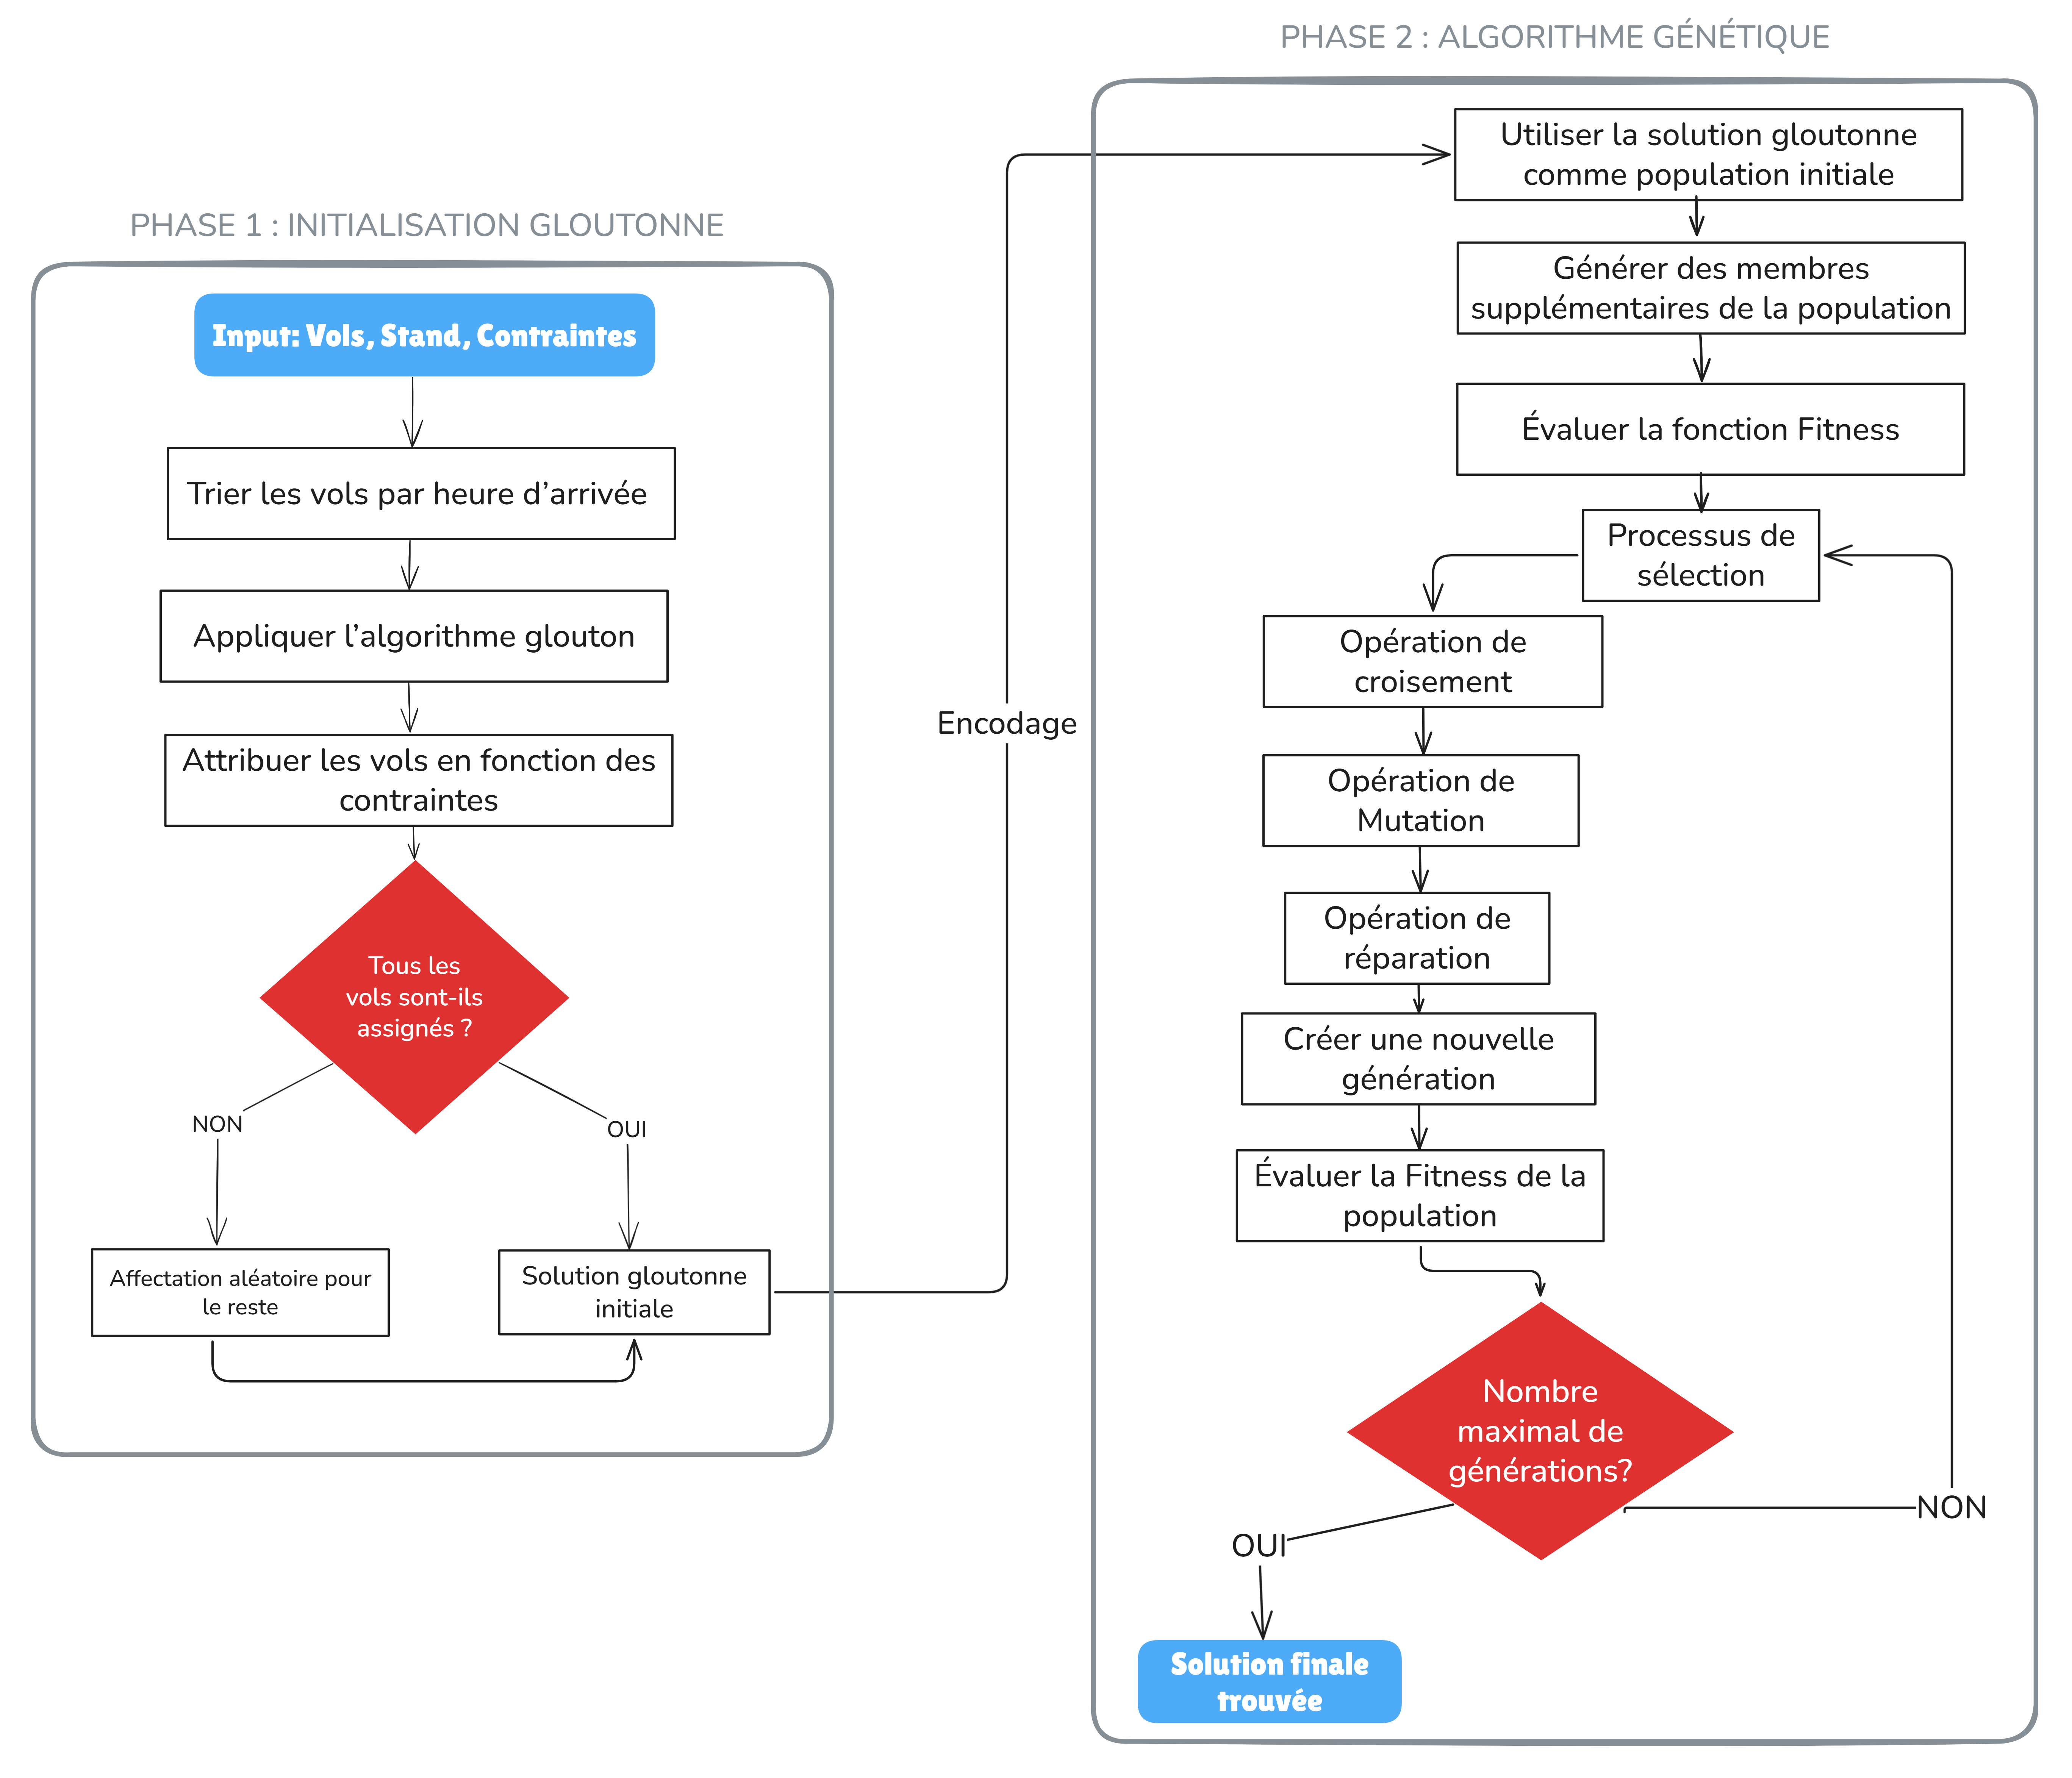
\includegraphics[width=0.9\linewidth]{assets/algo/GA_Algorithm.jpg}
	\caption{Organigramme de l'algorithme génétique}
	\label{fig:GGA}
\end{figure}
		\vspace{-0.7em}     
 Comme illustré dans la Figure~\ref{fig:GGA}, l’approche suit une structure en deux phases : la première utilise un algorithme glouton pour produire rapidement des solutions réalisables proches de l’optimal ; la seconde exploite ces solutions élites pour initialiser l’algorithme génétique, accélérant ainsi la convergence tout en améliorant la qualité des solutions.
 \vspace{-0.7em}
\subsubsection*{Approche d’hybridation}
\label{subsubsec:hybridization}

L’algorithme GGA associe la rapidité des heuristiques gloutonnes à la puissance d’optimisation des algorithmes génétiques.Cette hybridation crée un effet complémentaire dans lequel la composante gloutonne fournit des solutions initiales de qualité, et la composante évolutionnaire explore l’espace des solutions pour obtenir de meilleures affectations.

L’hybridation s’effectue en deux phases : d’abord, un algorithme glouton génère des solutions faisables en triant les vols et en appliquant des règles d’affectation basées sur les contraintes ; ensuite, ces solutions sont utilisées comme individus élites dans la population initiale de l’algorithme génétique, fournissant une base solide pour l’optimisation.
\vspace{-0.5em}
\paragraph{Initialisation par algorithme glouton}
La phase d’initialisation s’appuie sur des heuristiques gloutonnes pour générer des solutions de départ de qualité. Les vols sont triés par heure d’arrivée, et les stands sont affectés en tenant compte de la disponibilité et des contraintes de compatibilité. Cette approche permet à une grande partie de la population initiale de contenir des solutions valides et proches de l’optimum plutôt que des solutions aléatoires.

À l’issue de la première phase, la solution obtenue via l’algorithme glouton est encodée dans un format compatible avec celui attendu par l’algorithme génétique. Le mécanisme d’encodage, qui assure une transition fluide entre la représentation heuristique et celle en chromosomes, est détaillé dans la section~\ref{sssec:chromosome_encoding}.
\vspace{-0.7em}
\subsubsection{Encodage des Chromosomes}
\label{sssec:chromosome_encoding}

La représentation des chromosomes utilise un schéma d'encodage entier direct qui permet de mapper efficacement les vols aux stands.

\vspace{-0.7em}
\paragraph{Structure d’encodage}
Chaque chromosome est représenté par un vecteur d'entiers :

\begin{figure}[H]
	\centering
	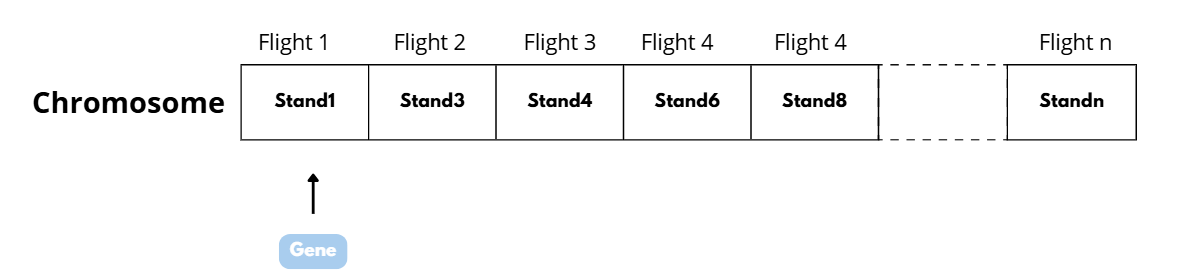
\includegraphics[width=0.9\linewidth]{assets/algo/Encodage.png}
	\caption{Structure de l’encodage}
	\label{fig:enter-label}
\end{figure}

Où :
\begin{itemize}
	\item $n$ = nombre total de vols,
	\item $Stand_i$ = indice du stand affecté au vol $i$ (gène $i$),
	\item La position $i$ correspond au vol $i$,
	\item Les valeurs des gènes vont de $0$ à $|Stands|-1$, selon le mapping (ex : B01 $\rightarrow$ 1, J01 $\rightarrow$ 2).
\end{itemize}

\paragraph{Représentation des gènes}
Chaque gène représente une affectation vol-stand :
\begin{itemize}
	\item \textbf{Indice du gène} : Position dans le chromosome (identifiant du vol),
	\item \textbf{Valeur du gène} : Entier représentant l’indice du stand dans la base,
	\item \textbf{Correspondance} : Association directe entre la valeur du gène et le stand.
\end{itemize}

\paragraph{Exemple d'encodage}
Pour les vols $F = [F_1, F_2, F_3, F_4]$ et les stands $S = [B01, C01, B02, E01, J01]$ :

\text{Chromosome}
\begin{figure}[H]
	\centering
	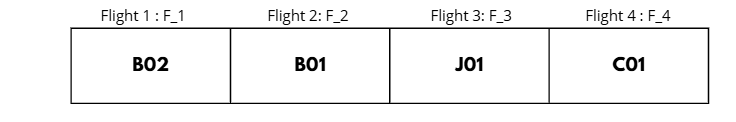
\includegraphics[width=0.7\linewidth]{assets/algo/Chr.png}
	\caption{Exemple d'encodage}
	\label{fig:enter-label}
\end{figure}
\vspace{-2em}
\begin{align}
	\text{Affectation} &= \{F_1 \rightarrow B02, F_2 \rightarrow B01, F_3 \rightarrow J01, F_4 \rightarrow C01\}
\end{align}

Cet encodage permet une efficacité computationnelle via l’indexation directe et prend naturellement en charge les opérations génétiques.

\paragraph{Processus de l’algorithme génétique}
Après l’initialisation, l’algorithme exécute les opérations génétiques standard jusqu’à satisfaction du critère d’arrêt.

\textbf{Critère d’arrêt :} l’algorithme s’arrête lorsque le nombre maximal de générations est atteint.

\paragraph{Sélection}
Les parents sont sélectionnés à l’aide d’une sélection par tournoi avec une probabilité définie, favorisant les individus avec une meilleure aptitude.

\paragraph{Croisement}
Un croisement en un point est appliqué avec une probabilité donnée. Un point de croisement aléatoire divise les chromosomes parents, permettant aux enfants d’hériter de matériel génétique des deux parents. Cela favorise la combinaison de schémas d’affectation efficaces.

\paragraph{Mutation}
La mutation s’applique avec une certaine probabilité, où un gène aléatoire est remplacé par une affectation de stand compatible. Cette opération introduit de la diversité et réduit les risques de convergence prématurée.

\paragraph{Mécanisme de réparation}
Après le croisement et la mutation, une procédure de réparation est lancée pour garantir que chaque individu respecte les contraintes du problème. Les affectations invalides causées par des conflits temporels, des incompatibilités ou des incohérences de zones sont identifiées et corrigées en réaffectant les vols vers le stand compatible le plus proche. Cette étape est essentielle pour assurer la validité des solutions tout au long de l’évolution.

\subsubsection*{Pseudocode de l’Algorithme GGA Hybride}

Le pseudocode suivant résume l’implémentation de l’algorithme génétique-glouton hybride, tel que présenté précédemment.

\begin{algorithm}[H]
	\caption{Algorithme Hybride Glouton-Génétique}
	\label{alg:gga_main}
	\begin{algorithmic}[1]
		\Require Vols $F$, Stands $S$, Contraintes $C$
		\Ensure Meilleure solution et score de fitness associé
		
		\Comment{Phase 1 : Initialisation gloutonne}
		\State Trier les vols par heure d’arrivée
		\State Générer une solution gloutonne à l’aide des règles d’affectation sous contraintes
		\State Créer la population initiale composée de variantes gloutonnes et de solutions aléatoires
		
		\Comment{Phase 2 : Évolution génétique}
		\State Initialiser la population avec les solutions gloutonnes
		\State Évaluer le score de fitness de la population initiale
		
		\While{not TerminationCriterion()}
		\Comment{Sélection}
		\State Sélectionner les parents selon la méthode de tournoi
		
		\Comment{Croisement}
		\State Générer les descendants par croisement à un point
		
		\Comment{Mutation}
		\State Appliquer une mutation pour introduire de la diversité
		
		\Comment{Réparation}
		\State Réparer les solutions non réalisables afin de respecter les contraintes
		
		\Comment{Remplacement}
		\State Remplacer la population par la nouvelle génération (avec préservation de l’élitisme)
		\State Évaluer le fitness de la nouvelle population
		\State Mettre à jour la meilleure solution si amélioration
		\EndWhile
		
		\Return Meilleure solution et valeur de fitness correspondante
	\end{algorithmic}
\end{algorithm}

%--------------------------------------------------

\section{Description des Hyperparamètres de l’Algorithme Génétique}
Cette section présente les principaux hyperparamètres utilisés dans notre approche hybride.

L’hybridation du glouton avec l’algorithme génétique utilise les hyperparamètres standards suivants :

\paragraph{Probabilité de mutation} Contrôle la probabilité d’introduire des modifications aléatoires dans une solution pour maintenir la diversité génétique et éviter la convergence prématurée vers des optima locaux.

\paragraph{Probabilité de croisement} Détermine la fréquence à laquelle le croisement entre deux parents est réalisé, équilibrant l’exploration de nouveaux espaces de solutions et l’exploitation des bonnes solutions existantes.

\paragraph{Taille de la population} Spécifie le nombre d’individus (solutions) maintenus à chaque génération. Une population plus grande améliore la diversité, mais augmente le coût de calcul.

\paragraph{Nombre de générations} Définit le nombre d’itérations de l’algorithme. Plus il y en a, plus l’exploration est profonde, mais cela allonge également le temps de traitement.

\section{Conclusion}
Ce chapitre a présenté la modélisation mathématique du problème d'affectation des vols aux stands, en s'appuyant sur une revue des approches existantes et leurs limites. Une formulation multi-objectifs a été proposée pour équilibrer l'utilisation des ressources et améliorer l'expérience passager. Nous avons également détaillé les paramètres, contraintes, et hyperparamètres associés à l’algorithme hybride glouton-génétique, en justifiant les choix méthodologiques adoptés.

Le prochain chapitre portera sur l’implémentation concrète du modèle proposé, les métriques d’évaluation, ainsi que l’analyse des résultats obtenus comparés aux affectations réelles.
	% \chapter{Implémentation et Déploiement}
\vspace{-1.5em}
\chaptertoc
\vspace{-2.5em}
\section{Introduction}
Ce chapitre présente les résultats obtenus à travers différentes métriques de performance, avant de traiter les aspects pratiques liés au déploiement du système ainsi que les interfaces développées pour en faciliter l’utilisation opérationnelle.
\vspace{-1.2em}
\section{Métriques d’Évaluation}
\vspace{-1em}
L’évaluation des performances des algorithmes d’affectation de stands nécessite un cadre d’analyse complet, intégrant à la fois l’efficacité opérationnelle et la performance algorithmique. Pour atteindre cet objectif, nous définissons deux catégories distinctes de métriques d’évaluation, offrant des perspectives complémentaires sur les performances des solutions proposées.

\subsection{Métriques de Validation des Performances}

La première catégorie regroupe des métriques visant à valider les performances de l’algorithme par rapport aux données opérationnelles réelles du \ac{SOAM}. Ces métriques mesurent à quel point les solutions générées par l’algorithme se rapprochent des décisions et contraintes opérationnelles.

\begin{enumerate}
	\item \textbf{Taux d’affectation des vols} : mesure le pourcentage de vols affectés avec succès à un stand, ce qui reflète la capacité de l’algorithme à gérer l’ensemble du programme de vols.
	\vspace{-1em}
	\begin{equation}
		\eta_{assigned} = \frac{|F_{assigned}|}{|F_{total}|} \times 100\%
	\end{equation}
	\vspace{-1em}
	\item \textbf{Taux de respect des contraintes} : évalue la proportion de contraintes opérationnelles respectées dans la solution finale, garantissant le respect des exigences de sécurité et d’exploitation.
	\vspace{-1em}
	\begin{equation}
		\gamma_{constraints} = \frac{|C_{satisfied}|}{|C_{total}|} \times 100\%
	\end{equation}
	
	\item \textbf{Utilisation des stands de contact} : quantifie l’efficacité d’utilisation des stands de contact, généralement préférés pour le confort des passagers.
	\vspace{-1em}
	\begin{equation}
		\rho_{contact} = \frac{|S_{contact}^{used}|}{|S_{contact}^{total}|} \times 100\%
	\end{equation}
	
	\item \textbf{Utilisation des stands éloignés} : mesure le taux d’utilisation des stands éloignés, fournissant une indication sur la répartition des ressources.
	\vspace{-0.7em}
	\begin{equation}
		\rho_{remote} = \frac{|S_{remote}^{used}|}{|S_{remote}^{total}|} \times 100\%
	\end{equation}
\end{enumerate}

\subsection{Métriques de Comparaison des algorithmes}

La seconde catégorie regroupe des métriques conçues pour comparer de manière systématique les performances relatives de différents algorithmes.

\begin{enumerate}
	\item \textbf{Stabilité des solutions} : évalue la régularité des résultats d’affectation sur plusieurs exécutions de l’algorithme avec les mêmes données d’entrée. Cette métrique est cruciale pour garantir que la solution finale soit fiable et réutilisable en environnement réel.
	\begin{equation}
		\sigma_{stable} = \frac{\text{Nombre d'affectations cohérentes}}{\text{Nombre total d'exécutions}} \times 100\%
	\end{equation}
	
	\item \textbf{Temps de calcul} : mesure la durée réelle d’exécution nécessaire pour obtenir une solution, indiquant l’adaptabilité de l’algorithme aux environnements en temps réel.
	\begin{equation}
		T_{exec} = t_{end} - t_{start}
	\end{equation}
	
	\item \textbf{Complexité temporelle} : représente la complexité computationnelle théorique de l’algorithme en fonction de la taille du problème.
	\vspace{-1em}
	\begin{equation}
		\mathcal{O}(f(n)) \quad \text{où } n = \text{taille du problème}
	\end{equation}
	\vspace{-2em}
	\item \textbf{Utilisation globale des ressources} : évalue l’efficacité de l’utilisation des stands disponibles, reflétant la capacité de l’algorithme à optimiser la gestion des ressources.
	\begin{equation}
		\mu_{\text{utilization}} = \frac{\sum_{g \in G} T_{\text{occupied}}(g)}{\sum_{g \in G} T_{\text{available}}(g)} \times 100\%
	\end{equation}
	
	Cette métrique est approfondie en comparant le nombre de stands utilisés par terminal et par type de vol (International vs Domestique), selon les différents algorithmes et l’affectation réelle observée.
	
	\begin{itemize}
		\item \textbf{Vols internationaux} : majoritairement affectés aux Terminaux 1 et 2, avec une préférence pour les stands proches de ces terminaux.
		\item \textbf{Vols domestiques} : généralement affectés au Terminal 1, avec une flexibilité pour être dirigés vers des stands plus éloignés si nécessaire.
	\end{itemize}
	
	Cette décomposition permet d’évaluer dans quelle mesure l’algorithme respecte les préférences opérationnelles et les schémas spécifiques à chaque terminal.
\end{enumerate}
\vspace{-1em}
\section{Détails de l’Implémentation}
 cette section décrit en détail l’implémentation de notre solution, incluant les choix d’algorithmes, les réglages des hyperparamètres et les considérations techniques liées à l’optimisation des performances.
\vspace{-0.8em}
\subsection{Cadre d’Optimisation des Hyperparamètres}

La méthodologie d’hybridation proposée a nécessité un processus rigoureux de sélection des hyperparamètres afin de garantir des performances algorithmiques optimales. Une stratégie complète de recherche par grille (\textbf{grid search}) a été mise en place pour explorer systématiquement l’espace des hyperparamètres, permettant ainsi d’identifier la configuration maximisant la qualité des solutions sur divers scénarios. Cette approche exhaustive garantit que les paramètres retenus sont statistiquement significatifs et théoriquement fondés.
\vspace{-0.5em}
\subsection{Configuration de l’Algorithme Génétique Glouton}

L’algorithme génétique glouton a été finement réglé à l’aide de \textbf{grid search}. Le processus d’optimisation a considéré quatre paramètres : la probabilité de croisement ($p_c$), la probabilité de mutation ($p_m$), la taille de la population ($N_{pop}$) et le nombre de générations ($N_{gen}$).

\textbf{Grid search} a permis d’identifier la configuration optimale suivante :
\begin{align}
	N_{pop} &= 4 \\
	N_{gen} &= 7 \\
	p_c &= 0{,}7 \\
	p_m &= 0{,}2
\end{align}

Ces paramètres ont été validés à travers des tests sur plusieurs instances du problème, garantissant la robustesse statistique et la généralisabilité de l’approche, tout en assurant un équilibre entre exploration et exploitation.
\vspace{-1em}
\subsection{Configuration du Recuit simulé et de la Recherche Tabou}
L’algorithme Hybridee a été configuré à l’aide de paramètres ajustés, afin d’équilibrer efficacement l’exploration de l’espace de recherche et la convergence vers des solutions de qualité.
\vspace{0.5em}
\textbf{Paramètres du recuit simulé (Simulated Annealing)} :
\vspace{-1em}
\begin{align*}
	\texttt{initial\_temperature}      &= 0.50 \\
	\texttt{cooling\_rate}             &= 0.99 \\
	\texttt{min\_temperature}          &= 0.05 \\
	\texttt{max\_iterations}           &= 5 \\
	\texttt{iterations\_per\_temp}     &= 5 \\
\end{align*}

\vspace{-2em}
\textbf{Paramètres de la recherche tabou (Tabu Search)} :
\vspace{-1em}
\begin{align*}
	\texttt{max\_iterations}           &= 5 \\
	\texttt{tabu\_size}                &= 5 \\
\end{align*}

\vspace{-2em}
Cette configuration assure un compromis raisonnable entre qualité de solution et temps de traitement.

\section{Résultats et Discussion}
\vspace{-0.7em}
Cette section présente une évaluation complète des algorithmes d’affectation de stands, en comparant leurs performances avec les affectations réelles, selon plusieurs métriques d’efficacité.
\vspace{-1em}
\subsection{Validation par Rapport aux Affectations Réelles}
\vspace{-0.5em}
Pour valider les approches algorithmiques, nous comparons tout d’abord les \textbf{algorithmes classiques} aux affectations de stands réelles, puis la \textbf{solution hybride} à l’affectation réelle (SOAM).
\vspace{-2em}
\subsubsection{\textcolor{darkblue}{Algorithmes Classiques vs. Affectations Réelles}}
Nous évaluons quatre approches fondamentales :
\begin{itemize}
	\item Algorithme classique
	\item Programmation linéaire (PL)
	\item Algorithme hongrois
	\item Algorithme glouton
\end{itemize}
\vspace{-0.7em}
\paragraph{Analyse de l’Utilisation des Ressources}



La comparaison des métriques clés est illustrée par les figures~\ref{fig:overall_utilization} et~\ref{fig:contact_and_remote}, qui présentent respectivement l’utilisation globale des ressources, et l’utilisation des stands de contact et éloignés.

\begin{figure}[H]
	\centering
	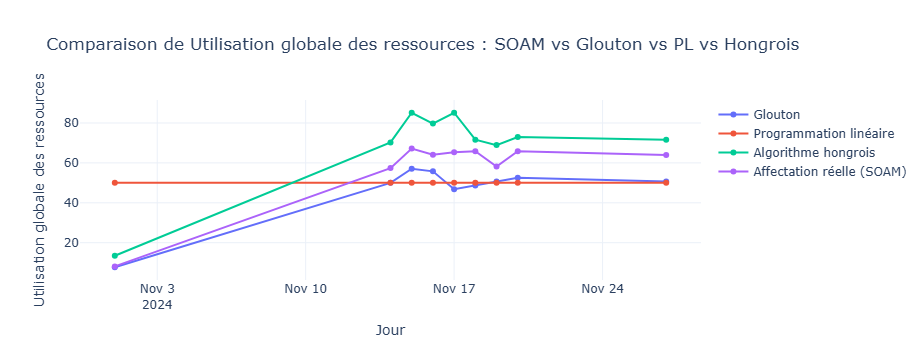
\includegraphics[width=0.8\linewidth]{assets/diagrams/overall_utilisation.png}
	\caption{Utilisation Globale des Ressources}
	\label{fig:overall_utilization}
\end{figure}


\begin{figure}[H]
	\centering
	\begin{minipage}{0.49\linewidth}
		\centering
		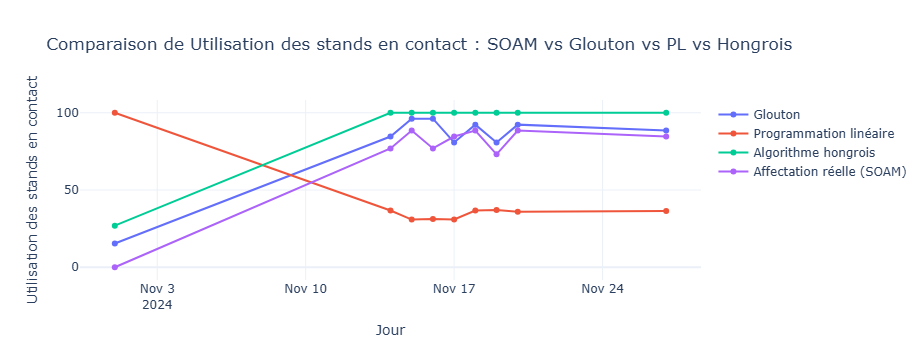
\includegraphics[width=\linewidth]{assets/diagrams/stand_contact.png}
		\caption{Utilisation des stands au contact}
		\label{fig:contact_utilization}
	\end{minipage}
	\hfill
	\begin{minipage}{0.49\linewidth}
		\centering
		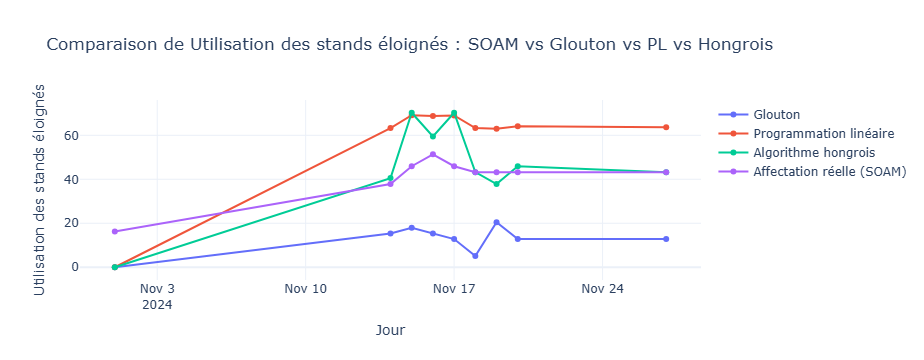
\includegraphics[width=\linewidth]{assets/diagrams/stand_eloigne.png}
		\caption{Utilisation des stands éloignés}
		\label{fig:remote_utilization}
	\end{minipage}
	\caption{Figure~\ref{fig:contact_and_remote}: Utilisation des stands de contact et des stands éloignés}
	\label{fig:contact_and_remote}
\end{figure}

\noindent
\textbf{Analyse :} D’après les figures, les approches algorithmiques – en particulier l’\textit{algorithme glouton} et l’\textit{algorithme hongrois} – surpassent nettement l’affectation réelle du \ac{SOAM} en maximisant l’utilisation des stands de contact. Ces méthodes permettent également une réduction notable de l’utilisation des stands éloignés, ce qui indique une meilleure efficacité des ressources. L’approche par \textit{programmation linéaire} performe également mieux que l’affectation réelle, mais reste en deçà des deux autres en termes d’utilisation optimale.

\paragraph{Répartition de l’Utilisation des Stands}

La figure~\ref{fig:stand_usage} montre la répartition des stands utilisés par terminal et type de vol (international vs. domestique), pour chaque méthode testée et l’affectation réelle.
\begin{figure}[H]
	\centering
	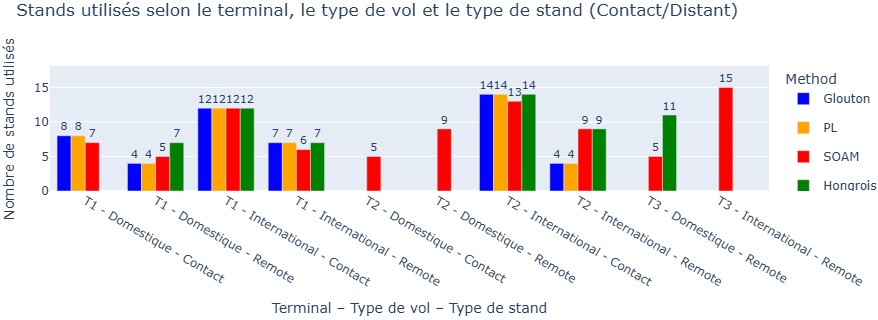
\includegraphics[width=1\textwidth]{assets/diagrams/terminal.jpg}
	\caption{Nombre de stands utilisés par terminal et type de vol selon les différents algorithmes et les affectations réelles.}
	\label{fig:stand_usage}
\end{figure}

\subsubsection{\textcolor{darkblue}{Comparaison Glouton vs. PL vs. Hongrois}}

Le tableau fournit une comparaison détaillée jour par jour en termes de temps d’exécution, coûts et métriques d’utilisation des ressources.
\begin{table}[htbp]
	\centering
	\caption{Comparaison des performances des algorithmes sur l’ensemble des jours de test}
	\label{tab:algorithm_comparison}
	\resizebox{\textwidth}{!}{%
		\begin{tabular}{|c|c|c|c|c|c|c|c|c|c|c|}
			\hline
			\multirow{2}{*}{\textbf{Jour}} & \multirow{2}{*}{\textbf{Vols}} & \multicolumn{3}{c|}{\textbf{Algorithme Hongrois}} & \multicolumn{3}{c|}{\textbf{Algorithme Glouton}} & \multicolumn{3}{c|}{\textbf{Programmation Linéaire}} \\
			\cline{3-11}
			& & \textbf{Temps (s)} & \textbf{Coût Total} & \textbf{Coût Moyen} & \textbf{Temps (s)} & \textbf{Coût Total} & \textbf{Coût Moyen} & \textbf{Temps (s)} & \textbf{Coût Total} & \textbf{Coût Moyen} \\
			\hline
			24-11-01 & 7 & 0.048 & \textbf{-280} & \textbf{-40.00} & \textbf{0.009} & \textbf{-280} & \textbf{-40.00} & 0.260 & \textbf{-280} & \textbf{-40.00} \\
			24-11-14 & 79 & \textbf{0.391} & -2000 & -25.31 & \textbf{0.126} & \textbf{-2420} & \textbf{-30.63} & 12.512 & -615 & -7.78 \\
			24-11-15 & 94 & \textbf{0.454} & -1715 & -18.24 & \textbf{0.172} & \textbf{-2960} & \textbf{-31.49} & 18.975 & -455 & -4.84 \\
			24-11-16 & 93 & 0.456 & -1835 & -19.73 & \textbf{0.156} & \textbf{-2465} & \textbf{-26.51} & 18.584 & -560 & -6.02 \\
			24-11-17 & 97 & 0.483 & -1730 & -17.83 & \textbf{0.153} & \textbf{-2935} & \textbf{-30.26} & 19.132 & -600 & -6.19 \\
			24-11-18 & 79 & 0.385 & -2050 & -25.63 & \textbf{0.151} & \textbf{-2775} & \textbf{-35.13} & 15.922 & -650 & -8.23 \\
			24-11-19 & 73 & 0.347 & -2095 & -28.69 & \textbf{0.099} & \textbf{-2115} & \textbf{-28.69} & 12.627 & -600 & -8.22 \\
			24-11-20 & 78 & 0.380 & -2040 & -26.15 & \textbf{0.128} & \textbf{-2535} & \textbf{-32.50} & 13.825 & -665 & -8.53 \\
			24-11-27 & 77 & 0.374 & -2040 & -26.49 & \textbf{0.114} & \textbf{-2515} & \textbf{-32.66} & 13.895 & -685 & -8.90 \\
			\hline
			\multicolumn{11}{|c|}{\textbf{Résumé de l’utilisation des ressources}} \\
			\hline
			\multicolumn{2}{|c|}{\textbf{Métrique}} & \multicolumn{3}{c|}{\textbf{Algorithme Hongrois}} & \multicolumn{3}{c|}{\textbf{Algorithme Glouton}} & \multicolumn{3}{c|}{\textbf{Programmation Linéaire}} \\
			\cline{3-11}
			\multicolumn{2}{|c|}{Util. Moyenne Stands Contact (\%)} & \multicolumn{3}{c|}{\textbf{91.88}} & \multicolumn{3}{c|}{84.73} & \multicolumn{3}{c|}{40.62} \\
			\multicolumn{2}{|c|}{Util. Moyenne Stands Distance (\%)} & \multicolumn{3}{c|}{\textbf{45.64}} & \multicolumn{3}{c|}{12.47} & \multicolumn{3}{c|}{62.37} \\
			\multicolumn{2}{|c|}{Taux d’Assignation (\%)} & \multicolumn{3}{c|}{\textbf{100}} & \multicolumn{3}{c|}{94} & \multicolumn{3}{c|}{\textbf{100}} \\
			\hline
		\end{tabular}
	}
\end{table}


L’évaluation expérimentale met en évidence les forces et limites de chaque algorithme. \textbf{L’algorithme hongrois} maximise l’usage des stands de contact (91{,}88\%), mais ne parvient pas à respecter tous les contraintes ( surtout la contrainte des stands incompatibles voir Annexe~\ref{tab:incompatibilites_stands}), en raison de sa contrainte de matrice carrée et de traitement par lot. \textbf{L’algorithme glouton} est le plus rapide (0{,}123s) et obtient les meilleurs coûts, mais son approche myope limite le taux d’affectation (94\%). \textbf{La programmation linéaire} assure une affectation complète (100\%) sans violation de contraintes, mais son temps d’exécution élevé (15{,}7s) réduit son applicabilité en temps réel.

Aucun algorithme ne présente un équilibre parfait entre efficacité, complétude d’affectation et utilisation des ressources. Ainsi, deux stratégies Hybridees sont proposées : une initialisation gloutonne rapide suivie d’un raffinement par algorithme génétique \ac{GA}, permettant de pallier les faiblesses individuelles tout en restant adaptée aux environnements dynamiques  et une autre combinant recuit simulé \ac{SA} et recherche tabou (TS), offrant une exploration efficace de l’espace des solutions avec un affinage local robuste.
\vspace{-1.7em}
\subsection{Comparaison Approfondie avec l’Affectation Réelle}

Cette section évalue les performances des approches hybrides combinant plusieurs stratégies d’optimisation.

\begin{itemize}
	\item Approche Hybridee Glouton+GA vs. Recuit simulé + Recherche tabou
	\item Comparaison avec les affectations réelles
\end{itemize}

\paragraph{Analyse de l’Utilisation des Ressources}

Les figures~\ref{fig:contact_and_remote_H} et~\ref{fig:overall_and_rate_H} comparent l’utilisation des stands (contact et éloignés) et la répartition des stands par terminal et type de vol.
\begin{figure}[H]
	\centering
	\begin{minipage}{0.49\linewidth}
		\centering
		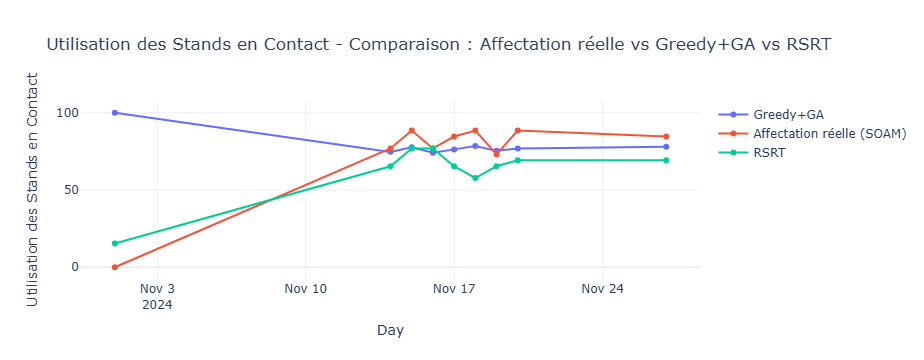
\includegraphics[width=\linewidth]{assets/diagrams/contactgasa.png}
		\caption{Utilisation des stands au contact
		}
		\label{fig:contact_utilization_H}
	\end{minipage}
	\hfill
	\begin{minipage}{0.49\linewidth}
		\centering
		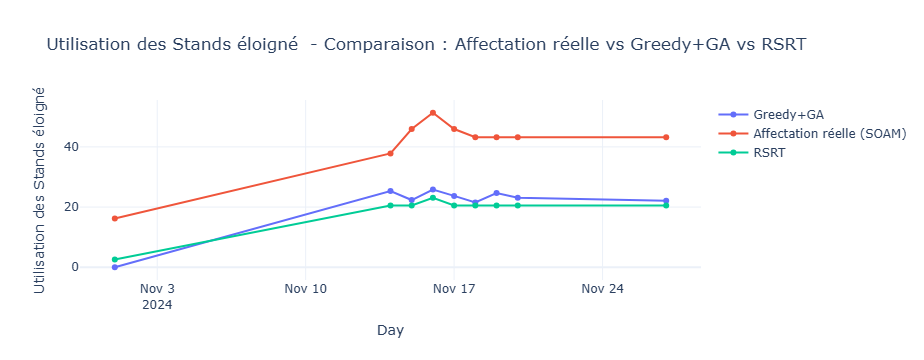
\includegraphics[width=\linewidth]{assets/diagrams/eloignegasa.png}
		\caption{Utilisation des stands éloignés
		}
		\label{fig:remote_utilization_H}
	\end{minipage}
	\caption{Figure~\ref{fig:contact_and_remote_H}: Utilisation des stands de contact et des stands éloignés.}
	\label{fig:contact_and_remote_H}
\end{figure}

\begin{figure}[H]
	\centering
	\begin{minipage}{0.49\linewidth}
		\centering
		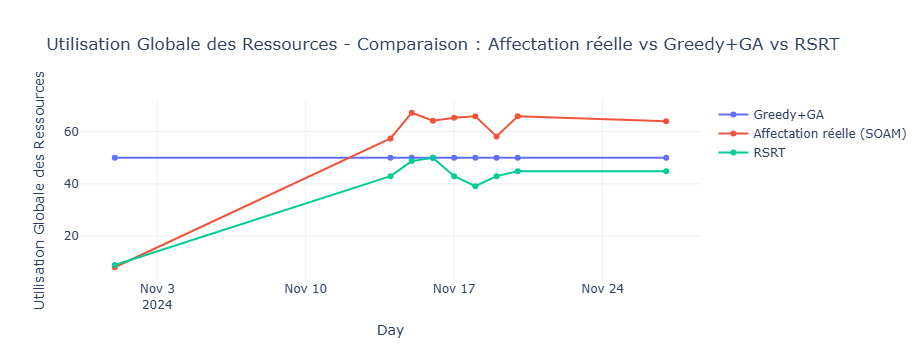
\includegraphics[width=\linewidth]{assets/diagrams/global_uti_gavssa.png}
		\caption{Utilisation globale des ressources}
		\label{fig:overall_utilization_H}
	\end{minipage}
	\hfill
	\begin{minipage}{0.49\linewidth}
		\centering
		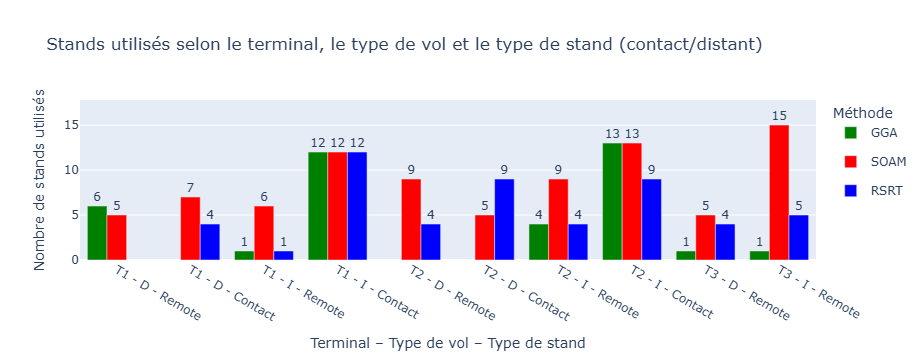
\includegraphics[width=\linewidth]{assets/diagrams/terminal_type.png}
		\caption{Taux d’affectation des vols}
		\label{fig:terminal_H}
	\end{minipage}
	\caption{Figure~\ref{fig:overall_and_rate_H}: Comparaison de l’utilisation globale et du taux d’affectation.}
	\label{fig:overall_and_rate_H}
\end{figure}


\subsubsection{Comparaison Glouton+GA vs. RSRT}

Le tableau~\ref{tab:RSRT_vs_gga} compare les performances de l’approche Hybridee Glouton + \ac{GA} et de l’approche Hybridee Recuit simulé + Recherche tabou .
\begin{table}[htbp]
	\centering
	\caption{Comparaison des performances : RSRT vs. Hybride Glouton+AG}
	\label{tab:RSRT_vs_gga}
	\resizebox{\textwidth}{!}{%
		\begin{tabular}{|c|c|c|c|c|c|c|c|}
			\hline
			\multirow{2}{*}{\textbf{Jour}} & \multirow{2}{*}{\textbf{Vols}} 
			& \multicolumn{3}{c|}{\textbf{RSRT (Recuit simulé + Recherche tabou)}} 
			& \multicolumn{3}{c|}{\textbf{Hybride Glouton+AG}} \\
			\cline{3-8}
			& & \textbf{Coût Total} & \textbf{Coût Moyen} & \textbf{Temps exéc. (s)} 
			& \textbf{Coût Total} & \textbf{Coût Moyen} & \textbf{Temps exéc. (s)} \\
			\hline
			01-11-2024 & 7  & -280   & -40.00  & 0.87       & \textbf{-2030}   & \textbf{-290.00}  & 0.4648 \\
			14-11-2024 & 79 & -2420  & -30.63  & 24.52      & \textbf{-195130} & \textbf{-2470.00} & 5.2960 \\
			15-11-2024 & 94 & -2960  & -31.49  & 25.39      & \textbf{-279650} & \textbf{-2975.00} & 6.7000 \\
			16-11-2024 & 93 & -2465  & -26.51  & 403.01     & \textbf{-273420} & \textbf{-2940.00} & 6.6312 \\
			17-11-2024 & 97 & -2935  & -30.26  & 35.37      & \textbf{-291000} & \textbf{-3000.00} & 7.3665 \\
			18-11-2024 & 79 & -2775  & -35.13  & 23.59      & \textbf{-201055} & \textbf{-2545.00} & 5.5957 \\
			19-11-2024 & 73 & -2115  & -28.97  & 28.26      & \textbf{-174105} & \textbf{-2385.00} & 4.9329 \\
			20-11-2024 & 78 & -2535  & -32.50  & 24.20      & \textbf{-198120} & \textbf{-2540.00} & 5.5983 \\
			27-11-2024 & 77 & -2515  & -32.66  & 20.09      & \textbf{-187110} & \textbf{-2430.00} & 5.3974 \\
			\hline
			\multicolumn{8}{|c|}{\textbf{Résumé de l’utilisation des ressources}} \\
			\hline
			\multicolumn{2}{|c|}{\textbf{Métrique}} 
			& \multicolumn{3}{c|}{\textbf{RSRT (Recuit simulé + Recherche tabou)}} 
			& \multicolumn{3}{c|}{\textbf{Hybride Glouton+AG}} \\
			\hline
			\multicolumn{2}{|c|}{Utilisation moyenne des stands contact (\%)} 
			& \multicolumn{3}{c|}{\textbf{69.43}} 
			& \multicolumn{3}{c|}{\textbf{76.83}} \\
			\multicolumn{2}{|c|}{Utilisation moyenne des stands distants (\%)} 
			& \multicolumn{3}{c|}{\textbf{18.76}} 
			& \multicolumn{3}{c|}{\textbf{22.06}} \\
			\multicolumn{2}{|c|}{Temps d’exécution moyen (s)} 
			& \multicolumn{3}{c|}{\textbf{65.71}} 
			& \multicolumn{3}{c|}{\textbf{5.33}} \\
			\hline
		\end{tabular}
	}
\end{table}

\section{Interprétation des résultats et justification du choix de l’algorithme}

L’analyse comparative entre l’algorithme RSRT (Recuit simulé + Recherche tabou) et l’algorithme Hybride Glouton+GA (GGA) met en évidence plusieurs points clés.

\subsection{Priorité à l’utilisation des stands contact}

L’utilisation moyenne des stands contact, qui représentent une ressource prioritaire pour le traitement rapide et efficace des vols, est significativement plus élevée avec GGA (76,83\,\%) qu’avec RSRT (69,43\,\%). Cette optimisation reflète la capacité de GGA à mieux respecter la priorité accordée aux stands contact par rapport aux stands distants, favorisant ainsi une meilleure qualité de service.

\subsection{Coût total et coût moyen}

Les résultats montrent que GGA permet d’obtenir des coûts totaux et moyens nettement inférieurs, traduisant une meilleure optimisation économique. Les coûts moyens tournent autour de -2500 pour GGA, contre environ -30 pour RSRT, ce qui souligne l’efficacité accrue de GGA dans l’affectation des ressources.

\subsection{Temps d’exécution}

Le temps d’exécution moyen de GGA est de 5,33 secondes, largement inférieur à celui de RSRT, qui est de 65,71 secondes. Cette différence est particulièrement importante dans un contexte opérationnel où la rapidité de prise de décision est essentielle. De plus, RSRT présente des pics de temps d’exécution très élevés, ce qui peut limiter son utilisation en temps réel.

\subsection{Justification du choix de l’algorithme Hybride Glouton + GA}

Compte tenu de ces résultats, l’algorithme Hybride Glouton + GA constitue un compromis optimal entre qualité de solution et efficacité temporelle. Il permet de :

\begin{itemize}
	\item Réduire significativement les coûts opérationnels,
	\item Respecter les priorités d’utilisation des stands, en maximisant l’utilisation des stands contact,
	\item Garantir un temps de calcul réduit, adapté à un environnement aéroportuaire dynamique nécessitant des décisions rapides.
\end{itemize}

Ainsi, GGA est la solution recommandée pour la gestion efficace des stands aéroportuaires, conciliant optimisation économique, respect des contraintes opérationnelles et performance temporelle. \textbf{Cette méthode sera adoptée pour son intégration avec l’interface Digital Twin, afin d’assurer une gestion en temps quasi-réel et optimisée des ressources aéroportuaires.}

\vspace{-1.3em}
\section{Intégration du modèle}
\vspace{-1em}
\subsection*{Informations Générales}
\begin{itemize}
	\item \textbf{Environnement :} \url{http://localhost:8000}
	\item \textbf{Date des tests :} \textcolor{darkblue}{16-06-2025}
	\item \textbf{Outils Utilisés :} \textcolor{darkblue}{FastAPI, Swagger UI}
	\item \textbf{Base de données :}\textcolor{darkblue}{ Fichiers CSV (\texttt{all\_flights.csv}, \texttt{stand.csv})}
	
\end{itemize}
\vspace{0.15cm}
Cette API permet de faire l'affectation des vols aux stands disponibles dans un aéroport en fonction de diverses contraintes et paramètres.Les principaux objectifs de cette évaluation sont :
\begin{itemize}
	\item La performance et le temps de réponse de l'API
	\item La gestion des erreurs et des cas limites :
	\begin{itemize}
		\item Évaluer comment l'API gère les erreurs en cas de saisie incorrecte, de champs manquants ou de valeurs non valides
		\item Assurer que des messages d'erreur clairs et appropriés sont retournés
	\end{itemize}
\end{itemize}

\vspace{-1.3em}
\subsection*{Méthodologie de Test}
Cette partie décrit la méthodologie utilisée pour tester les fonctionnalités de l’API.
\vspace{-1em}
\subsubsection{Entrées du système}

\fcolorbox{black!20}{gray!5}{
	\begin{minipage}{\linewidth}
		\texttt{\textcolor{darkblue}{\{}}\\
		\hspace*{1em}\texttt{\textcolor{darkblue}{"date": "2024-11-01",}}\\
		\hspace*{1em}\texttt{\textcolor{darkblue}{"start\_time": "08:00",}}\\
		\hspace*{1em}\texttt{\textcolor{darkblue}{"end\_time": "18:00"}}\\
		\texttt{\textcolor{darkblue}{\}}}
	\end{minipage}
}
\vspace{0.15cm}

\begin{itemize}
	\item \textbf{date} : La date pour laquelle l’affectation doit être réalisée, au format \texttt{YY-MM-DD} (ISO)
	\item \textbf{start\_time} : Heure de début de la plage horaire au format 24h (\texttt{HH:MM})
	\item \textbf{end\_time} : Heure de fin de la plage horaire au format 24h (\texttt{HH:MM})
\end{itemize}
\vspace{-0.5em}
\subsubsection{Tests fonctionnels des endpoints}
\vspace{-0.7em}
Le tableau~\ref{tab:tests-endpoints} présente une série de tests effectués sur les différents endpoints de l’API. Chaque requête est testée pour valider la réponse attendue, tant sur le contenu que sur le format.
\vspace{-1em}
\begin{table}[H]
	\centering
	\renewcommand{\arraystretch}{0.6}
	\caption{Tests fonctionnels des endpoints principaux de l’API}
	\begin{tabularx}{\textwidth}{p{3.3cm} p{3.5cm} p{3.5cm} p{4.6cm}}
		\toprule
		\textbf{Endpoint} & \textbf{Description} & \textbf{Résultat attendu} & \textbf{Résultat obtenu} \\
		\midrule
		\texttt{GET /} &
		Vérification de la racine de l'API &
		Message de bienvenue &
		\texttt{\{"message": "Welcome to Airport Stand Assignment API"\}} \\
		
		\midrule
		\texttt{GET /available-dates/} &
		Récupération des dates disponibles &
		Liste des dates contenues&
		Liste correctement reçue \\
		
		\midrule
		\texttt{POST /assign-stands/} &
		Affectation des vols pour une journée &
		Résultat JSON avec durée de traitement &
		Réponse structurée avec les données affectées \\
		
		\bottomrule
	\end{tabularx}
	\label{tab:tests-endpoints}
\end{table}

\vspace{-1.7em}


\subsubsection{Tests de performance}

Pour une évaluation approfondie, trois journées aux trafics variés ont été choisies afin de tester le système dans différentes conditions:
\begin{itemize}
	\item nombre de vols minimal \textcolor{darkblue}{(jour avec seulement 1 vol)},
	\item nombre de vols moyen \textcolor{darkblue}{(jour avec 70 vols)},
	\item nombre de vols maximal \textcolor{darkblue}{(jour avec 97 vols)}.
\end{itemize}

Les tests ont été exécutés sur l'ensemble de la journée \textcolor{darkblue}{(de 00:00 à 23:59)} afin de capturer toutes les variations possibles de performance selon les plages horaires.

Le tableau~\ref{tab:tests-performance} résume les résultats obtenus, avec le temps de réponse mesuré pour chaque cas.

\begin{table}[H]
	\centering
	\renewcommand{\arraystretch}{0.9}
	\caption{Performance de l’API en fonction du volume de vols à traiter}
	\begin{tabularx}{\textwidth}{l l l X X}
		\toprule
		\textbf{Date} & \textbf{Heure début} & \textbf{Heure fin} & \textbf{Nombre de vols} & \textbf{Temps de réponse (s)} \\
		\midrule
		24-11-03 & 00:00 & 23:59 & 1 & Pas d'affectation \\
		24-11-01 & 00:00 & 23:59 & 8 & 0.95 \\
		24-11-12 & 00:00 & 23:59 & 70 & 4.95 \\
		24-11-17 & 00:00 & 23:59 & 97 & 8.05 \\
		\bottomrule
	\end{tabularx}
	\label{tab:tests-performance}
\end{table}

\noindent
\textit{Remarque :} Lorsqu'une seule rotation est enregistrée dans une journée, aucune affectation de stand n’est effectuée, car aucune succession n’est possible.

\subsubsection{Tests de validation et gestion des erreurs}
Le tableau~\ref{tab:erreurs-api} illustre une série de cas de test validant la gestion des erreurs par l'API. Il couvre généralement les principaux cas limites.
\vspace{-1em}
\begin{table}[H]
	\centering
	\renewcommand{\arraystretch}{0.5}
	\caption{Exemples de scénarios d'erreurs et messages retournés par l'API}
	\vspace{-0.5em}
	\begin{tabularx}{\textwidth}{l X X}
		\toprule
		\textbf{Scénario} & \textbf{Données en entrée} & \textbf{Message retourné} \\
		\midrule
		Format de date invalide &
		\texttt{\{"date": "14-11-2024", "start\_time": "08:00", "end\_time": "18:00"\}} &
		Format de date invalide. Utilisez le format AA-MM-JJ \textcolor{darkblue}{(ex: 24-11-14)}. \\
		
		\midrule
		Format d'heure invalide &
		\texttt{\{"date": "24-11-14", "start\_time": "8h00", "end\_time": "18:00"\}} &
		Le format de l'heure doit être HH:MM en 24h \textcolor{darkblue}{(ex: 14:30)}. \\
		
		\midrule
		Dates hors plage &
		\texttt{\{"date": "24-10-01", "start\_time": "08:00", "end\_time": "18:00"\}} &
		Les dates suivantes ne sont pas présentes dans le jeu de données : \textcolor{darkblue}{24-10-01}. \\
		
		\midrule
		Date manquante &
		\texttt{\{"date": " ", "start\_time": "08:00", "end\_time": "18:00"\}} &
		La date ne peut pas être vide. \\
		
		\midrule
		Mois invalide &
		\texttt{\{"date": "24-13-01", "start\_time": "08:00", "end\_time": "18:00"\}} &
		Le mois doit être entre 01 et 12, reçu 13. \\
		
		\midrule
		Jour invalide &
		\texttt{\{"date": "24-10-40", "start\_time": "08:00", "end\_time": "18:00"\}} &
		Le jour doit être entre 01 et 31, reçu 40. \\
		
		\midrule
		Heure de début > heure de fin &
		\texttt{\{"date": "24-11-14", "start\_time": "18:00", "end\_time": "08:00"\}} &
		L'heure de début doit être antérieure à l'heure de fin. \\
		
		\bottomrule
	\end{tabularx}
	\label{tab:erreurs-api}
\end{table}


\subsection*{Mécanismes internes du système}

Le système repose sur deux mécanismes clés pour optimiser le traitement.

\begin{itemize}
	\item \textbf{Mécanisme de mise en cache :} Réutilisation directe des résultats précédemment calculés.
	\item \textbf{Traitement temporel :} Affectation journalière suivie d’un filtrage par intervalle.
\end{itemize}
\vspace{-1.5em}
\subsection{Qualité des affectations}

Le tableau~\ref{tab:qualite-affectations} évalue la qualité des affectations pour trois journées à fort trafic, en indiquant la répartition des types de stands et le taux de compatibilité avion/stand.

\begin{table}[H]
	\centering
	\renewcommand{\arraystretch}{1}
	\caption{Qualité des affectations par date : répartition des stands et compatibilité}
	\begin{tabularx}{\textwidth}{l c c c c}
		\toprule
		\textbf{Date} & \textbf{Nb. de vols} & \textbf{Stands Contact} & \textbf{Stands Remote} & \textbf{Compatibilité avion/stand} \\
		\midrule
		24-11-12 & 70 & 18 & 7 & 100\% \\
		24-11-14 & 80 & 20 & 8 & 100\% \\
		24-11-17 & 97 & 16 & 14 & 100\% \\
		\bottomrule
	\end{tabularx}
	\label{tab:qualite-affectations}
\end{table}


\textbf{Chevauchement temporel :} Aucun



L’algorithme d’affectation génère un fichier au format JSON, où chaque vol est associé à un stand en fonction des contraintes opérationnelles et physiques. Un extrait représentatif de ce fichier est présenté ci-dessous.

L’intégralité du résultat d’affectation pour les journées testées est fournie en annexe, accompagnée de la signification de chaque attribut utilisé dans le fichier (cf. Table~\ref{tab:attributs_vols_complet}).

L’API respecte les objectifs fonctionnels fixés. L’algorithme propose des affectations pertinentes, conformes aux contraintes, avec une répartition équilibrée entre stands de contact et éloignés, et un taux de compatibilité avion/stand satisfaisant. 


\section{Réalisation}
Cette section présente les interfaces principales de l'application développée.

\subsection*{Visualisation des indicateurs de performance (KPI)}

Cette capture d'ecran presente 
L’interface développée intègre une section dédiée à la visualisation des \textbf{indicateurs de performance clés} (KPI), permettant de suivre et d’analyser en temps réel l’efficacité opérationnelle de l’affectation des stands avion.

L’image ci-dessous illustre cette interface de pilotage. Chaque encart correspond à un indicateur spécifique, calculé selon des règles métiers définies avec le client. Ces indicateurs ont pour objectif d’aider les décideurs à mieux comprendre l’utilisation des ressources, à identifier les retards ou anomalies, et à prendre des mesures correctives en cas de besoin.
\begin{figure}[H]
	\centering
	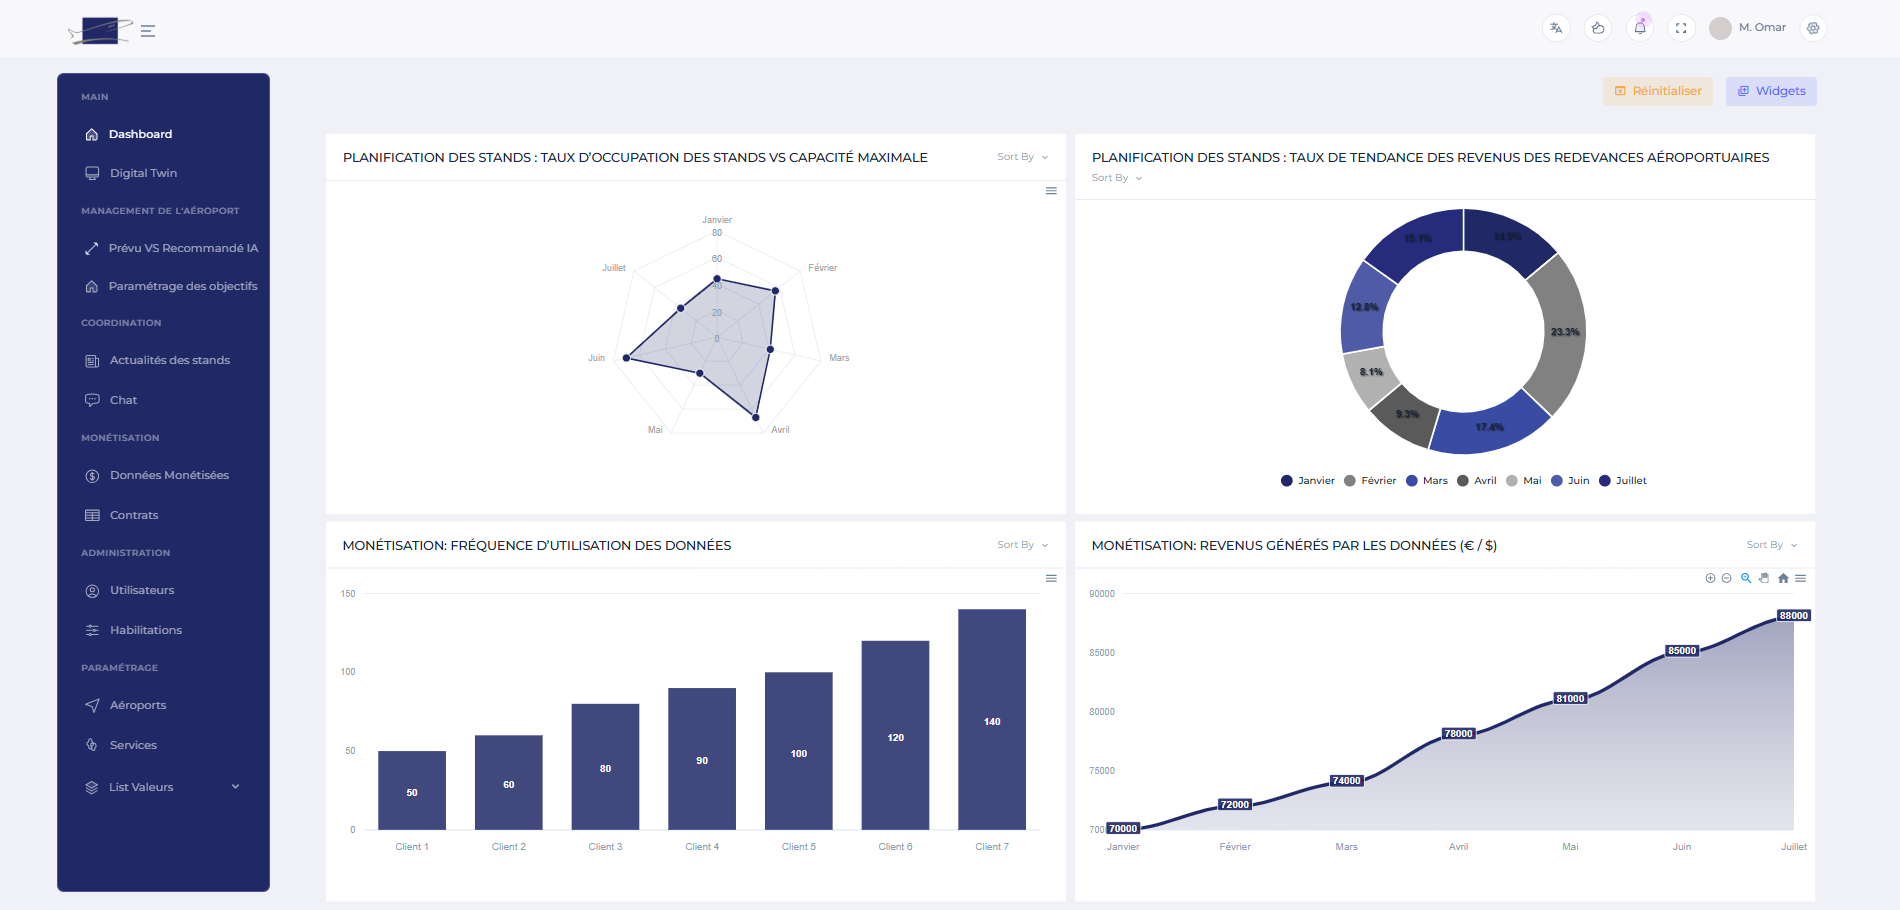
\includegraphics[width=0.95\textwidth]{assets/interfaces/kpi.png} % remplace par ton nom de fichier
	\caption{Interface de visualisation des KPI}
	\label{fig:kpi_interface}
\end{figure}

\subsection*{Fonctionnalité de recherche d’avion ou de stand}

L’une des fonctionnalités du jumeau numérique est la \textbf{recherche d’un avion ou d’un stand}, dans lequel l’utilisateur peut saisir : \textit{un matricule d’avion} ou \textit{un numéro de stand}


\begin{figure}[H]
	\centering
	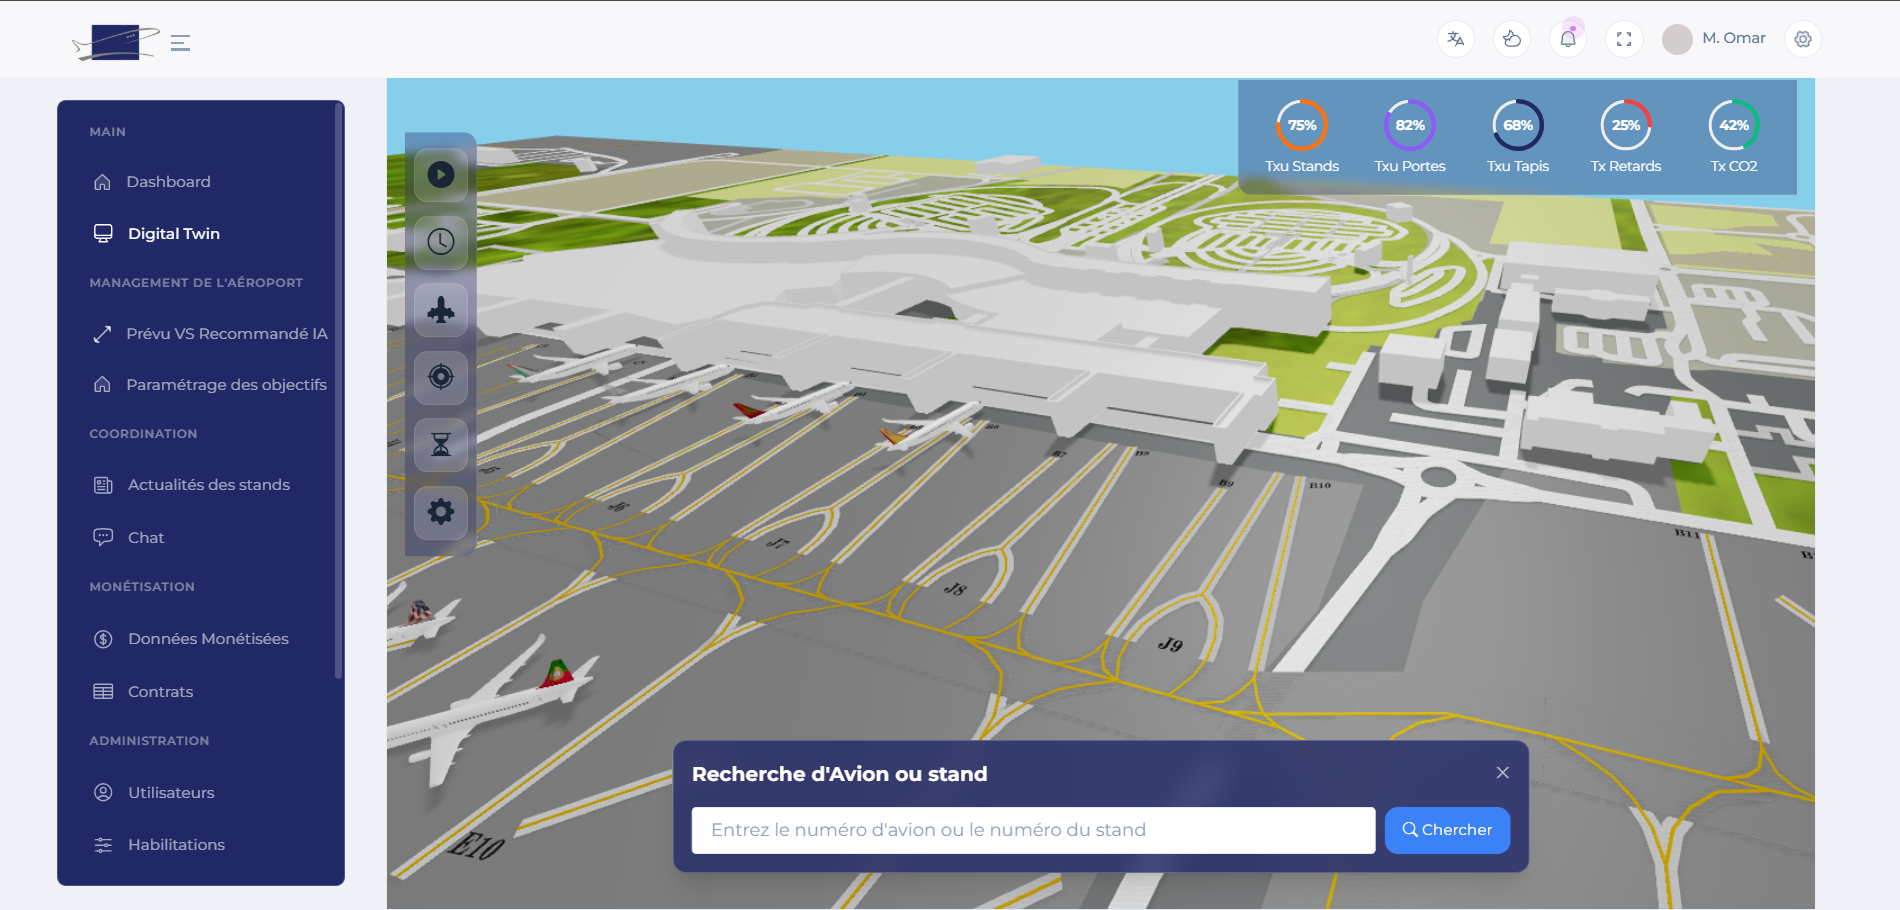
\includegraphics[width=0.95\textwidth]{assets/interfaces/recherche.png}
	\caption{Recherche d’un avion ou d’un stand avec affichage d’informations contextuelles}
	\label{fig:search_avion_stand}
\end{figure}
Une fois la recherche lancée, le système effectue une requête interne qui recentre automatiquement la vue 3D sur l’objet ciblé (avion ou stand) et affiche une fiche d’information contextuelle contenant plusieurs détails : matricule de l’avion, numéro du stand, statut du vol (ex.~: À l’heure), compagnie aérienne (ex.~: Spain Air), provenance (ex.~: New York (JFK)), marque de l’avion (ex.~: Airbus) et nombre de passagers (ex.~: 220).
\begin{figure}[H]
	\centering
	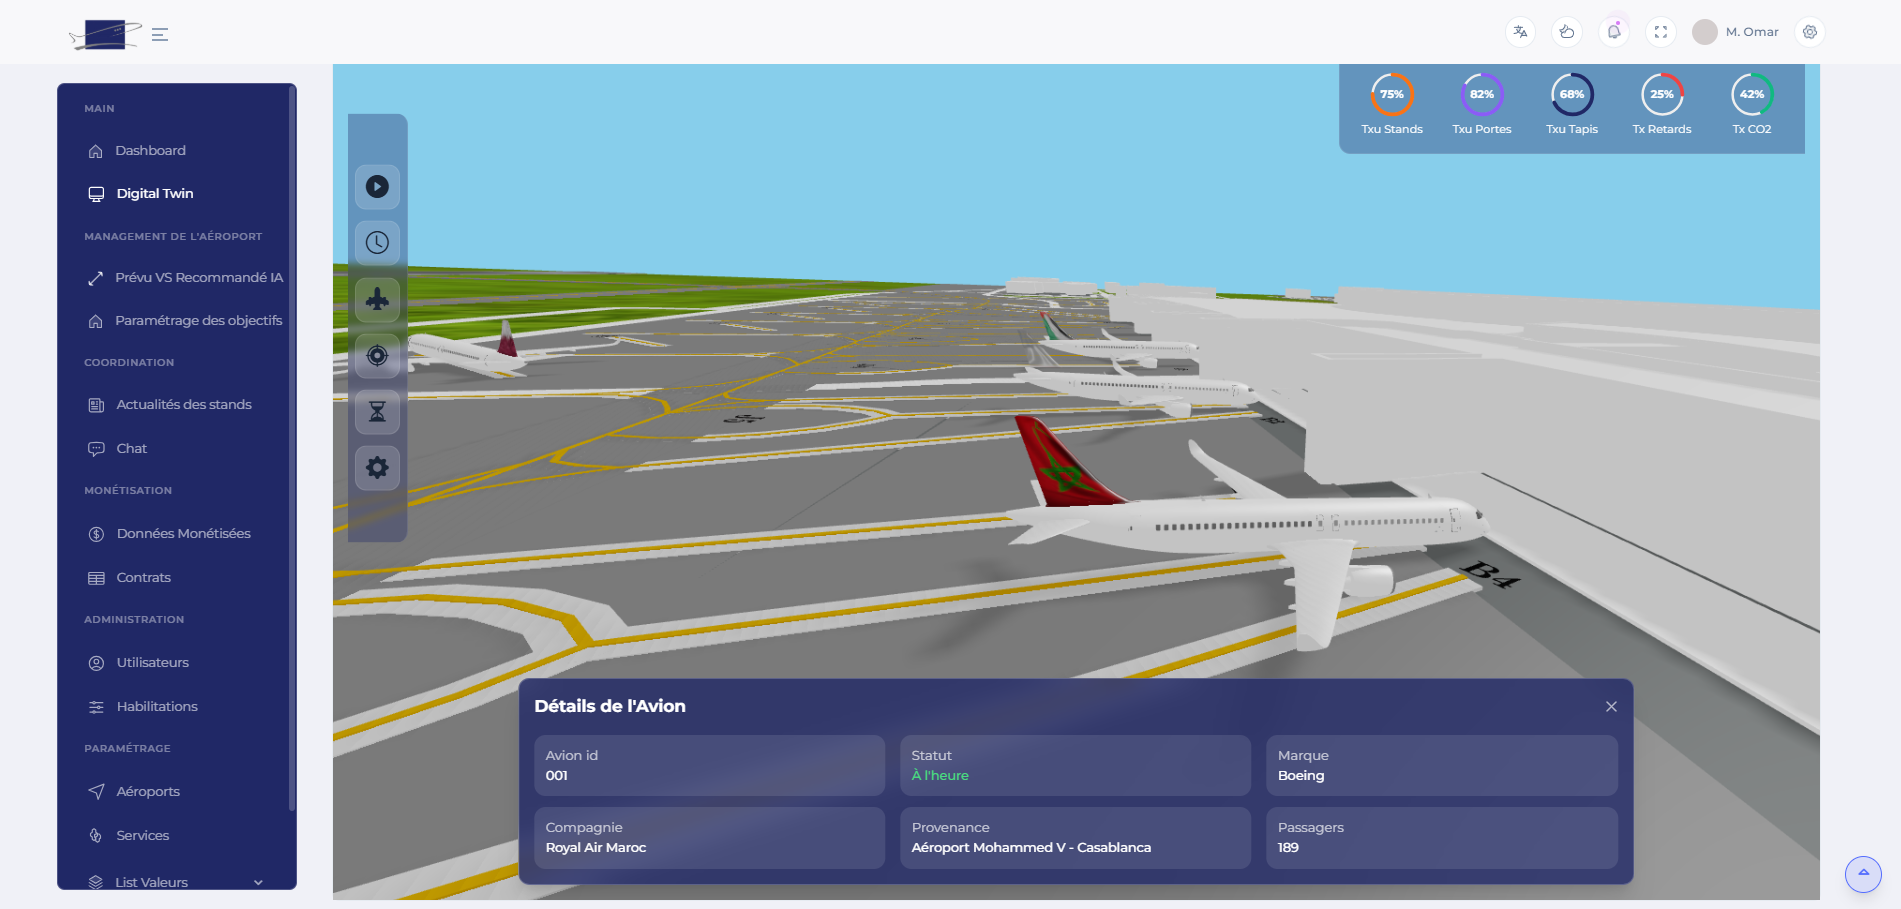
\includegraphics[width=0.85\textwidth]{assets/interfaces/affichageRecherche.png} % Remplace par ton image réelle
	\caption{Recherche d’un avion ou d’un stand avec affichage d’informations contextuelles}
	\label{fig:search_avion_stand}
\end{figure}

\subsection*{Simulation d’une journée d’activité passée}

L’interface du jumeau numérique permet aux utilisateurs de \textbf{simuler une journée d’activité antérieure} afin d’analyser le déroulement des opérations passées, détecter d’éventuelles anomalies, et évaluer la performance globale de l’aéroport.

Cette fonctionnalité se déroule en plusieurs étapes illustrées ci-dessous :

\begin{enumerate}
	\item \textbf{Sélection de la plage horaire}~: l’utilisateur choisit une date et une plage horaire. 
	\begin{figure}[H]
		\centering
		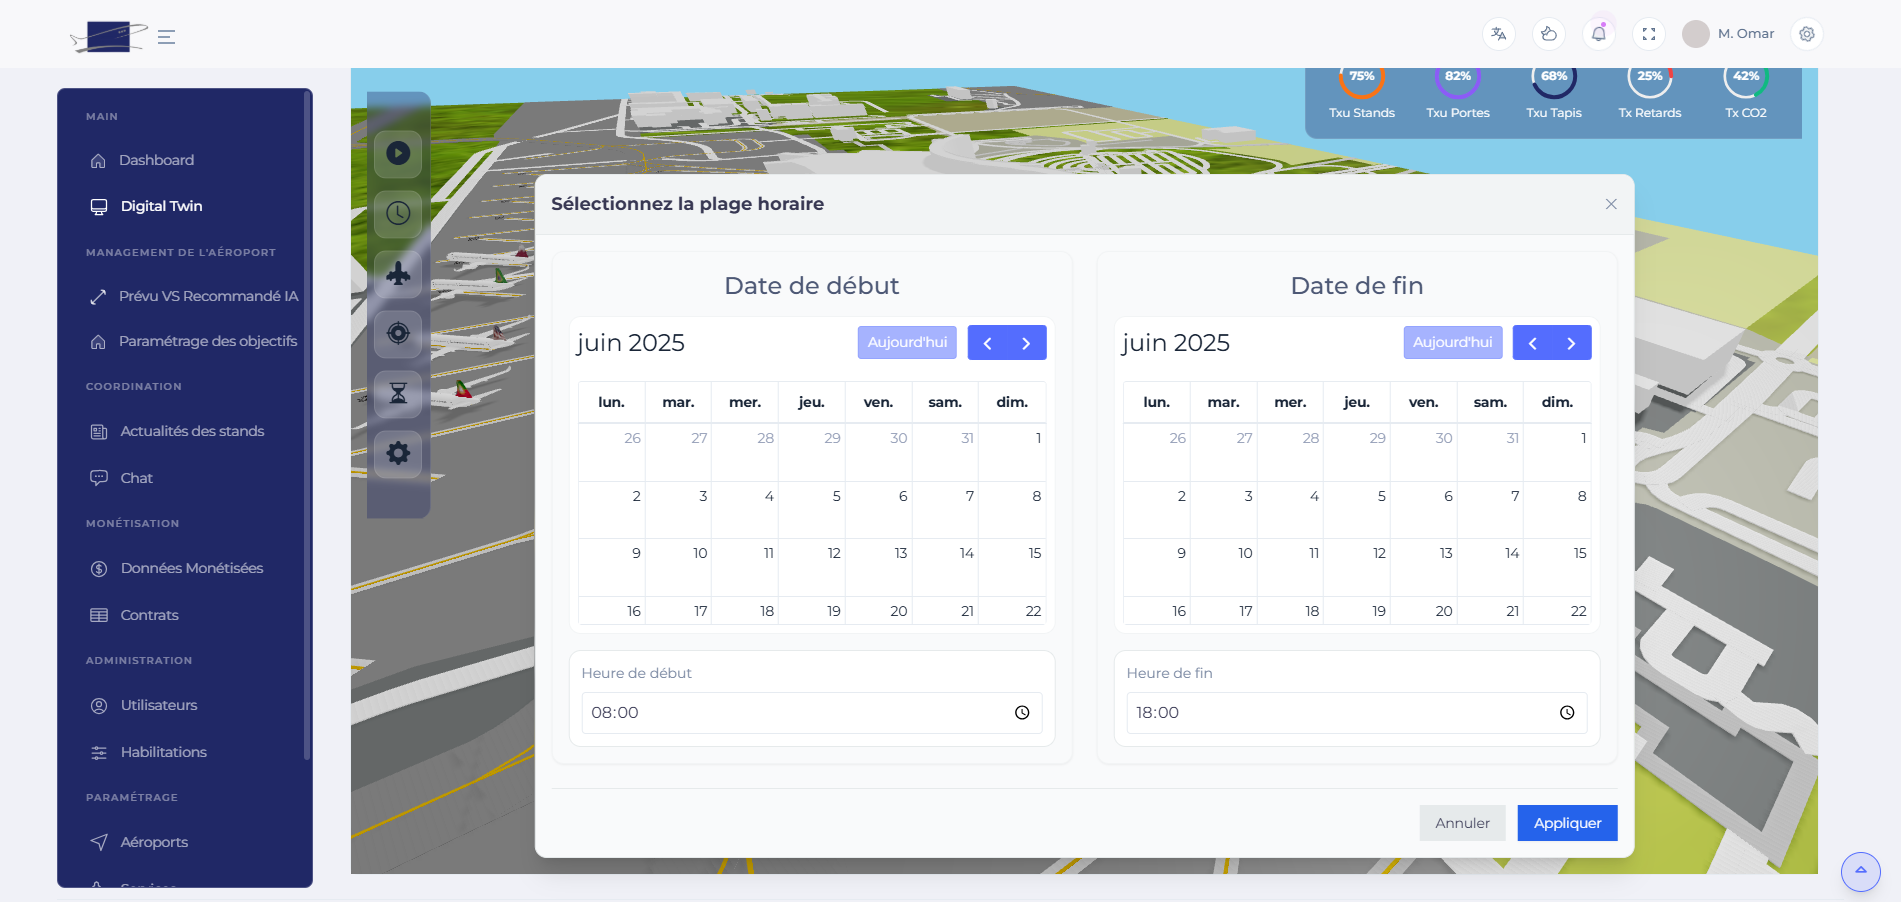
\includegraphics[width=0.95\textwidth]{assets/interfaces/simulation.png}
		\caption{Choix de la plage horaire pour la simulation d'une journée passée}
		\label{fig:simulation1}
	\end{figure}
	
	\item \textbf{Lancement de la simulation}~: une fois les paramètres validés, le système informe l’utilisateur que la simulation est en cours d’exécution.

	
	\item \textbf{Lecture de la simulation}~: l’activité de l’aéroport s’anime dans l’interface 3D sous forme de lecture chronologique. L’utilisateur peut ainsi visualiser l’évolution des vols, les affectations aux stands, les retards, les conflits, ou les événements inattendus.
	

\end{enumerate}

Cette fonctionnalité constitue un outil d’analyse puissant, permettant de \textbf{rejouer des scénarios passés} pour mieux comprendre les dysfonctionnements.
\subsection*{Mise à jour de la planification recommandée}

L’interface du jumeau numérique permet de comparer deux niveaux de planification~:

\begin{itemize}
	\item \textbf{L’affectation prévisionnelle}~: il s’agit de la planification effective des vols et des ressources réalisée par le \ac{SOAM}.
	
	\item \textbf{La planification recommandée}~: elle est générée dynamiquement par le moteur d’optimisation.
\end{itemize}

Une interface dédiée permet aux utilisateurs de visualiser ces deux plannings côte à côte, facilitant ainsi l’analyse des écarts entre le scénario initial et la recommandation opérationnelle.
\begin{figure}[H]
	\centering
	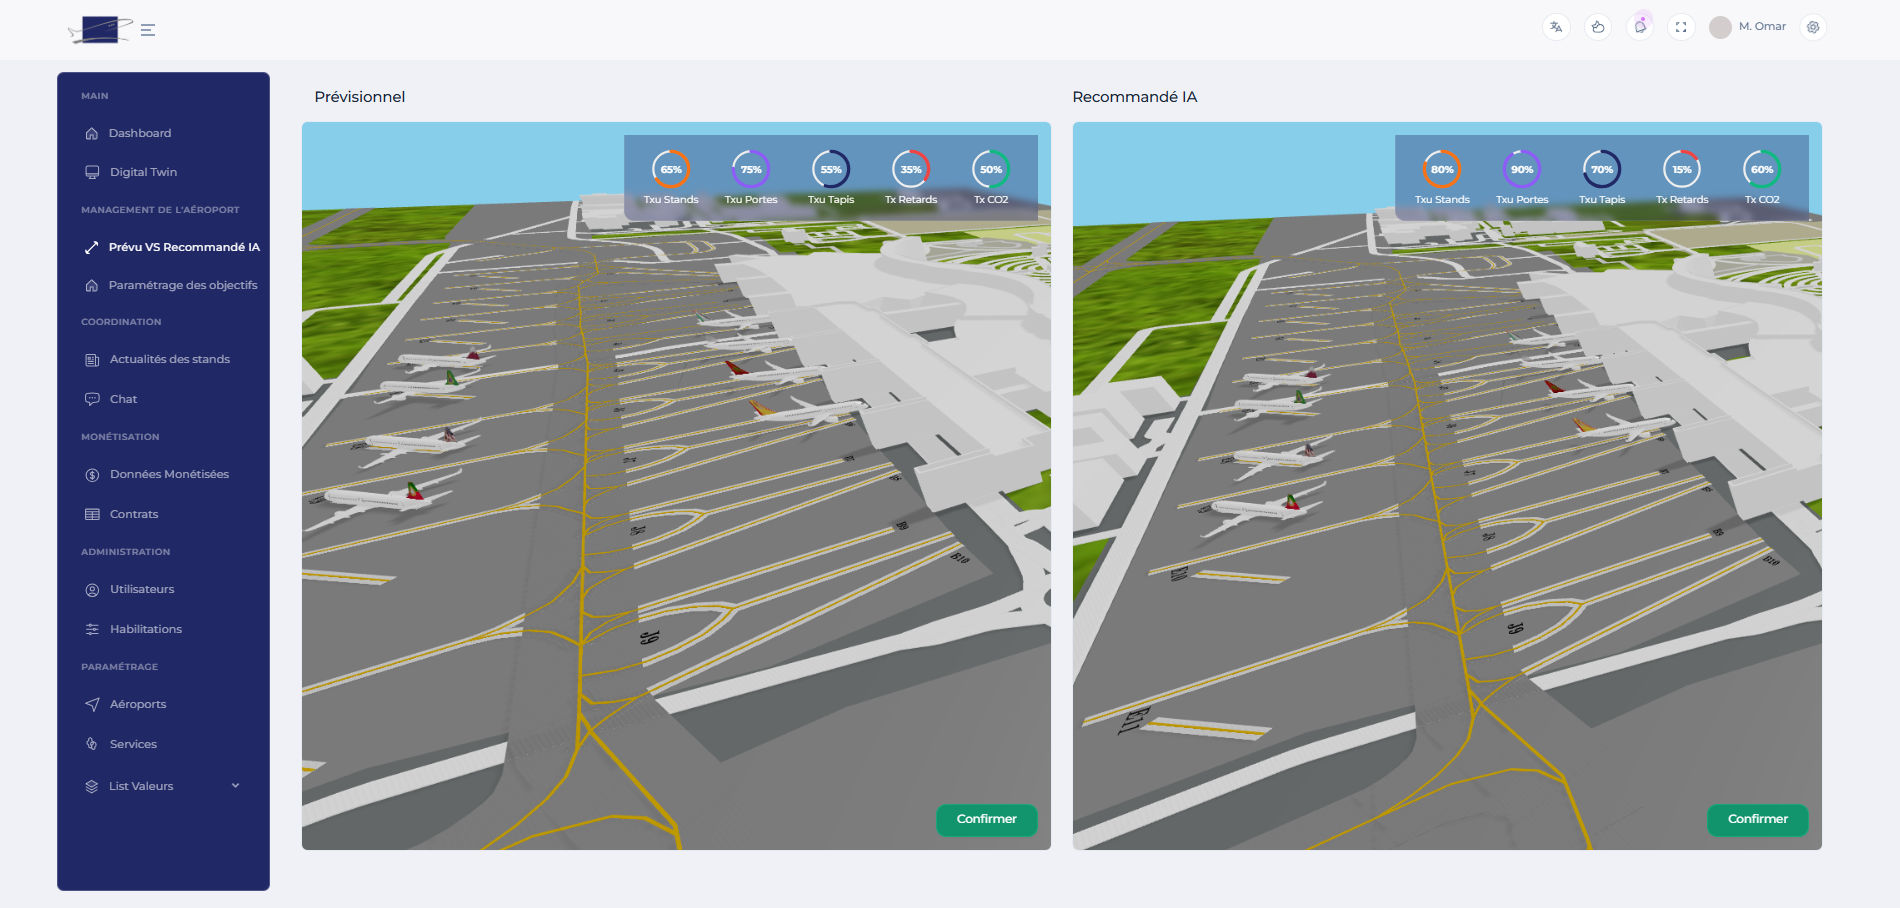
\includegraphics[width=0.95\textwidth]{assets/interfaces/comparaison.png} % Remplacer par ton image réelle
	\caption{Comparaison entre planification prévisionnelle et recommandée dans l’interface}
	\label{fig:planning_comparaison}
\end{figure}

\subsubsection*{Fonctionnalité 4 : Alertes et notifications}

L’interface dédiée au coordinateur intègre un système d’alertes et de notifications permettant d’améliorer la réactivité face aux événements critiques ou aux anomalies.

\begin{figure}[H]
	\centering
	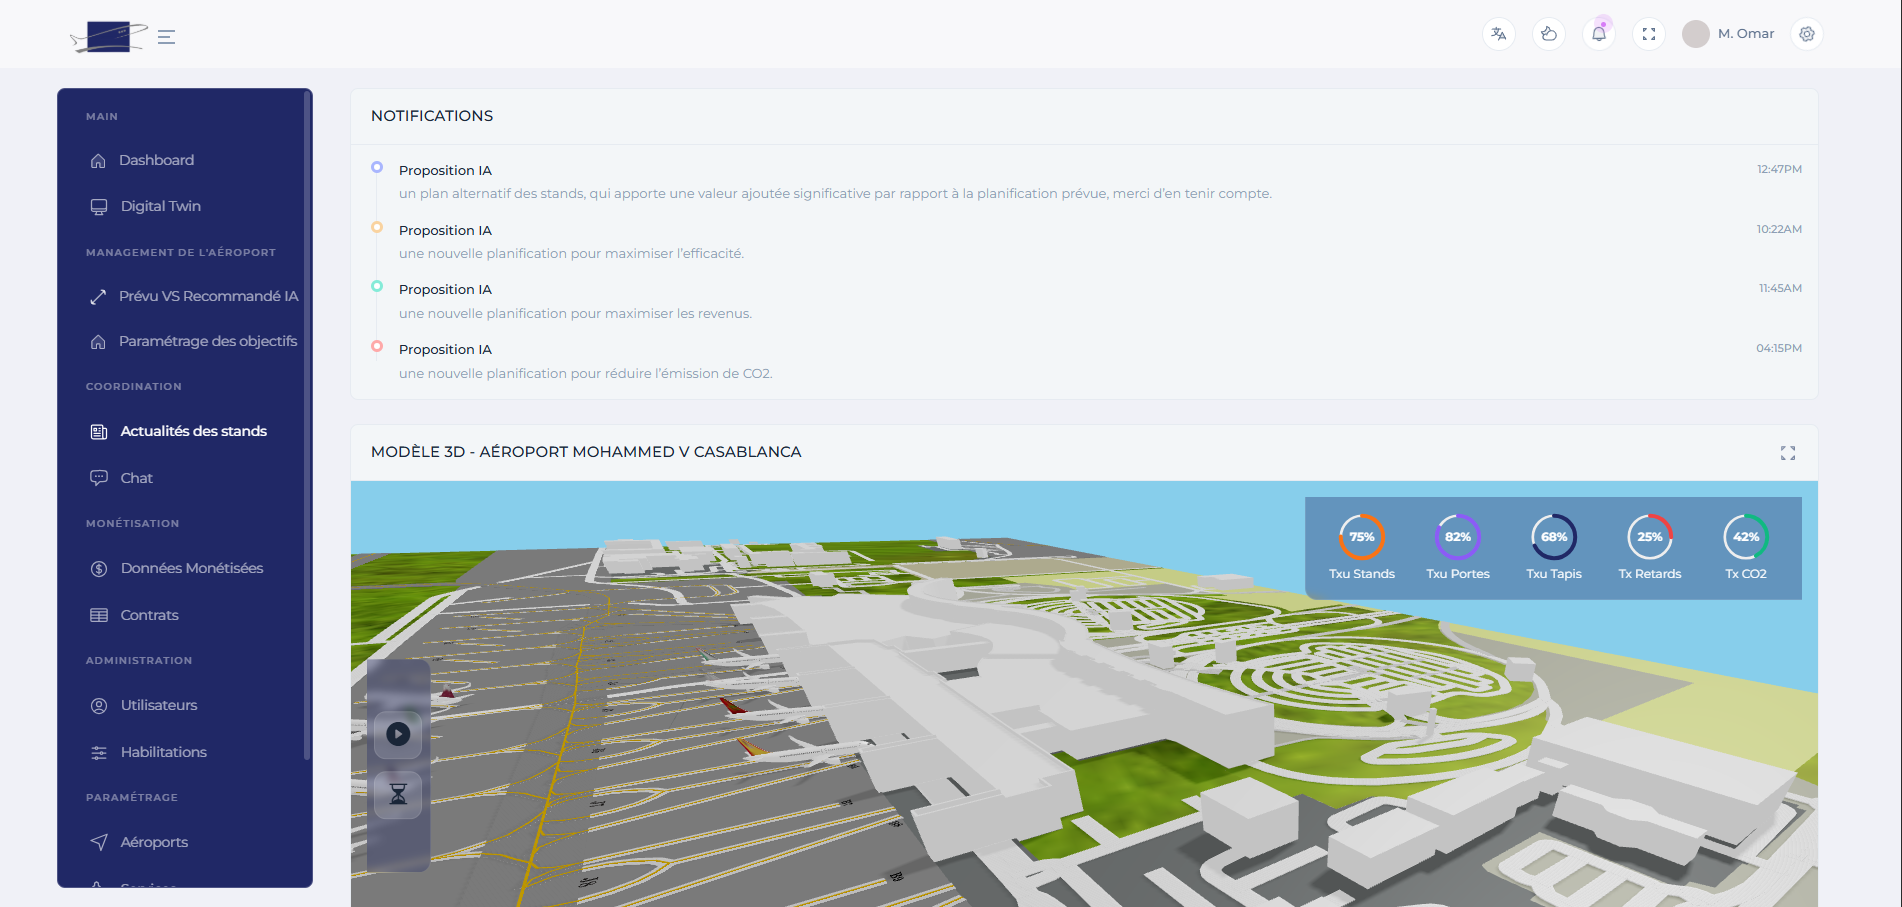
\includegraphics[width=0.95\textwidth]{assets/interfaces/alerte.png} % Remplace par ton image de notification
	\caption{Interface coordinateur : exemple d’alerte en cas de retard critique}
	\label{fig:alertes_notifications}
\end{figure}


\section{Conclusion}

Ce chapitre a présenté l’implémentation et le déploiement de notre solution d’affectation dynamique des stands. Après avoir défini les métriques d’évaluation, plusieurs approches algorithmiques ont été testées, dont le recuit simulé, la recherche tabou, l’algorithme glouton et l’algorithme génétique.

Les résultats ont montré que la combinaison de l’approche gloutonne et de l’algorithme génétique permet d’obtenir un bon équilibre entre coût, occupation optimale des stands contact et temps d’exécution. Cette approche hybride a donc été retenue comme module final du système.

Le modèle a été intégré dans une architecture complète, avec une interface de simulation, fournissant ainsi un outil intelligent d’aide à la décision adapté aux contraintes du domaine aéroportuaire.


	\include{chapters/revue}
	

 	\chapter*{Conclusion Générale}
\addcontentsline{toc}{chapter}{Conclusion Générale}
\vspace{-1.5cm}

Ce projet de fin d’études, réalisé au sein de l’entreprise \textbf{BI NewVision} en partenariat avec l’\textbf{\ac{ONDA}}, s’inscrit dans une dynamique de modernisation des aéroports marocains. Il porte sur le développement d’un \textbf{jumeau numérique} pour optimiser l’affectation des stands avion, en intégrant les contraintes métier et les aléas liés au trafic aérien.


Pour mener à bien ce projet, nous avons commencé par une analyse approfondie du dataset fourni, afin de mieux comprendre les données opérationnelles disponibles et d’en extraire les caractéristiques essentielles pour la modélisation. Cette phase a permis d’identifier des schémas comportementaux et de préparer les données à des fins de simulation et d’optimisation.

Le \ac{SAP} a été modélisé en intégrant plusieurs contraintes réelles telles que la compatibilité avion-stand, les conflits d’occupation et les restrictions d’adjacence. Nous avons défini une fonction objectif multicritère, puis testé différentes approches algorithmiques, exactes et heuristiques, évaluées selon des métriques comme la qualité des affectations, la robustesse et le temps de calcul.

Par la suite, nous avons mis en place une \textbf{architecture microservices}, intégrant un moteur d’optimisation via une API Python, couplé à une interface 3D permettant de simuler les affectations.


Ce projet m’a permis de développer des compétences techniques et méthodologiques variées, notamment en modélisation mathématique, algorithmique, ingénierie logicielle, traitement de données, ainsi qu’en gestion agile de projet au sein d’une équipe interdisciplinaire.

\vspace{1em}

Malgré l’avancement significatif du projet, plusieurs axes d’amélioration restent envisageables pour enrichir et renforcer la solution proposée. Nous envisageons les perspectives suivantes :

\begin{itemize}
	\item Finalisation de l'intégration complète de la solution dans l’environnement client.
	\item Ajout de nouveaux modules fonctionnels comme la gestion des bagages.
	\item Finalisation de l’intégration Cloudera pour l’exploitation directe des données
	\item Enrichissement du dataset pour affiner les performances des algorithmes.
	\item Intégration de contraintes supplémentaires spécifiques aux besoins évolutifs de l’ONDA.
\end{itemize}

Ces perspectives offrent un potentiel réel de développement pour rendre la solution encore plus complète, flexible et adaptable aux futurs besoins du client.

%En conclusion, ce projet de PFE a été une expérience enrichissante et stimulante, nous permettant de développer une application mobile novatrice utilisant la reconnaissance vocale pour guider les touristes à Marrakech. Nous avons relevé plusieurs défis tout au long du processus, tels que le scraping de données pour obtenir des informations précieuses, ainsi que l'adaptation de notre modèle de reconnaissance vocale à plusieurs langues avec de bons résultats.

%L'utilisation de technologies telles que Python, Java et la reconnaissance vocale nous a permis de repousser nos limites et de mieux comprendre les aspects techniques de leur intégration. De plus, nous avons exploré des fonctionnalités hors ligne pour assurer une expérience utilisateur fluide, même sans connexion Internet.  

%\noindent

%Ce projet nous a permis d'acquérir de nouvelles compétences en matière de développement d'applications mobiles avec le machine learning, de travailler avec des technologies émergentes et de résoudre des problèmes complexes. Nous avons également réalisé l'importance de l'encadrement, et nous tenons à exprimer notre profonde gratitude envers nos encadrants pour leur soutien et leurs encouragements tout au long du projet.

%En termes d'impacts potentiels, notre application peut contribuer à améliorer l'expérience touristique à Marrakech en offrant un guide vocal personnalisé et en facilitant la découverte de la ville pour les visiteurs. 

%Grosso modo, ce projet a été une étape importante dans notre parcours universitaire, nous permettant de mettre en pratique nos connaissances et de repousser les frontières de nos compétences. Nous sommes fiers des résultats obtenus.

%Cependant, même avec les fonctionnalités actuelles de notre application, il existe encore plusieurs perspectives intéressantes pour son amélioration. Nous envisageons les perspectives suivantes :
%\begin{itemize}
    %\item Généralisation de l'application pour toutes les villes du Maroc.
    %\item Intégration d'un système de réservation directement dans l'application pour faciliter et centraliser les réservations d'hébergements, de visites guidées, de restaurants, etc.
    %\item Ajout d'une fonctionnalité de chat intégrée permettant aux utilisateurs de contacter directement les responsables des hôtels, des restaurants, et autres établissements pour obtenir des informations, des recommandations ou une assistance personnalisée.
    %\item Intégration d'une carte géographique hors ligne pour permettre aux utilisateurs de naviguer facilement dans la ville de Marrakech sans dépendre d'une connexion Internet constante.
    %\item Mise en place d'un historique des activités pour permettre aux utilisateurs de consulter leurs activités passées, les lieux visités, les commentaires laissés, etc.

%\end{itemize}
 %   Ces perspectives ouvrent la voie à des améliorations futures de notre application et à des fonctionnalités encore plus avancées. Nous sommes impatients de poursuivre notre travail et d'explorer ces possibilités pour offrir aux touristes une expérience de voyage encore plus immersive et pratique à Marrakech.%






















 	% \renewcommand{\bibname}{Références}
 	% \bibliography{references}
 	% \chapter*{Annexes}
\addcontentsline{toc}{chapter}{Annexes}
\vspace{-1.2cm}

\section*{Macroplanning du projet}
Le projet s’étale sur une période de 22 mois et se décline en plusieurs phases successives visant à concevoir et implémenter un système d’optimisation pour la planification des stands avion. À ce jour, le projet est dans sa phase de \textbf{cadrage}, qui vise à affiner les objectifs, analyser les besoins et poser les fondations techniques.

\begin{figure}[H]
	\centering
	
\includegraphics[width=\linewidth]{assets/Annexe/macroplanning.png}
	\caption{Macroplanning global du projet}
	\label{fig:macrolplannning}
\end{figure}



\section*{Plan de l’aéroport CMN}
Le plan ci-dessous illustre la disposition des zones de stationnement à l’aéroport Mohammed V (CMN). Il a été utilisé comme base pour la modélisation des contraintes spatiales dans l’algorithme d’affectation.

\begin{figure}[H]
	\centering
	\rotatebox{90}{% rotation de 90° vers la gauche
		
\includegraphics[width=0.9\textheight]{assets/Annexe/plan.png}
	}
	\caption{Plan des zones de stationnement à l’aéroport Mohammed V (CMN)}
	\label{fig:plan}
\end{figure}




\section*{Contraintes d’incompatibilité entre stands}
Certains stands ne peuvent pas être utilisés simultanément, notamment ceux du type \texttt{J (Julia)}, qui imposent des restrictions sur les stands adjacents afin de garantir la sécurité et d’éviter les conflits opérationnels.

\begin{table}[H]
	\centering
	\renewcommand{\arraystretch}{1}
	\caption{Exemples de relations d'incompatibilité entre les stands}
	\begin{tabular}{|p{4cm}|p{6cm}|}
		\hline
		\textbf{Stand principal} & \textbf{Stands incompatibles} \\
		\hline
		J01 & C01, C02 \\
		J02 & C03, C04 \\
		J03 & C05, C06 \\
		J04 & C07, C08 \\
		J05 & B01, B02 \\
		J06 & B03, B04 \\
		J07 & B05, B06 \\
		J08 & B07, B08 \\
		J09 & B09, B10 \\
		J15 & C24, C25 \\
		\hline
	\end{tabular}
	\label{tab:incompatibilites_stands}
\end{table}


\noindent\textit{Remarque :} Lorsqu’un stand \texttt{J} est occupé, les stands listés comme incompatibles doivent être laissés vacants pour éviter toute interférence.


\section*{Exemple d'affectation de vols}
L’algorithme d’affectation génère un fichier JSON, où chaque vol est associé à un stand selon les contraintes et critères définis. Voici un extrait représentatif :

\begin{lstlisting}[language=json, 
	caption={Extrait du fichier JSON d’affectation}, 
	label={lst:json-result}, 
	basicstyle=\ttfamily\small, 
	breaklines=true,
	frame=single
	]
	"assignments": [{
		"VID": "290850832",
		"FLC": "Transavia France",
		"REG": "FHTVS",
		"DES": "RAK",
		"ORG": "ORY",
		"Aircraft_Type": "Boeing 737-800 (High Gross Weight)",
		"DAY_ARR": "2024-11-01",
		"DAY_DEP": "2024-11-01",
		"AIRCRAFT_SIZE": "Medium",
		"STAND": "C07",
		"Stand_Type": "Contact",
		"Max_Aircraft_Size": "Medium",
		"HEURE_VOL_ARR": "08:04",
		"HEURE_VOL_DEP": "08:49",
		"PXU_DEP": "189",
		"PXU_ARR": "189",
		"TERMINAL": "T1",
		"Vol_Type": "I"
	}]

\end{lstlisting}

\noindent Une visualisation de l’occupation des stands sur trois jours est également générée sous forme de diagramme de Gantt.


\section*{Chronologie d’Affectation des Vols aux Stands – Jour 19}

Le diagramme ci-dessous présente le diagramme de Gantt correspondant aux résultats de l’affectation des vols aux stands pour le jour 19, obtenus à l’aide de l’approche hybride combinant une heuristique gloutonne avec un algorithme génétique. Cette représentation visuelle illustre la répartition temporelle de l’occupation des stands et met en évidence l’efficacité de la méthode proposée pour gérer l’allocation des ressources sous contraintes opérationnelles.


\vspace{-1em}
\begin{figure}[H]
	\centering
	
\includegraphics[width=1.1\linewidth]{assets/Annexe/affectation.png}
	\caption{Diagrammes de gantt des stands}
	\label{fig:ganttStand}
\end{figure}

\section*{Signification des attributs utilisés}
Le tableau ci-dessous décrit les principaux attributs utilisés dans le jeu de données de vols.

\begin{table}[H]
	\scriptsize
	\renewcommand{\arraystretch}{1.3}
	\caption{Description des attributs du fichier d’affectation des vols}
	\begin{tabularx}{\textwidth}{@{} p{3cm} p{2.5cm} X p{3.3cm} @{}}
		\toprule
		\textbf{Catégorie} & \textbf{Attribut} & \textbf{Description} & \textbf{Exemple / Type} \\
		\midrule
		\multirow{2}{*}{Identification du vol} 
		& \texttt{VID} & Identifiant unique du vol & 290850832 \\
		& \texttt{FLC} & Nom de la compagnie aérienne & Transavia France \\
		
		\midrule
		\multirow{4}{*}{Informations temporelles} 
		& \texttt{DAY\_ARR / DEP} & Dates d’arrivée et de départ & 2024-11-01 \\
		& \texttt{HEURE\_VOL\_ARR / DEP} & Horaires du vol & 08:04, 08:49 \\
		& \texttt{VOL\_TYPE} & Type de vol (I/D) & I : International \\
		
		\midrule
		\multirow{3}{*}{Informations avion} 
		& \texttt{REG} & Immatriculation de l’avion & FHTVS \\
		& \texttt{AIRCRAFT\_TYPE} & Modèle commercial & Boeing 737-800 \\
		& \texttt{AIRCRAFT\_SIZE} & Taille de l’aéronef & Medium \\
		
		\midrule
		\multirow{4}{*}{Informations aéroportuaires} 
		& \texttt{ORG / DES} & Aéroports origine/destination & ORY / RAK \\
		& \texttt{STAND} & Stand attribué & C07 \\
		& \texttt{STAND\_TYPE} & Type de stand & Contact \\
		& \texttt{TERMINAL} & Terminal assigné & T1 \\
		
		\midrule
		\multirow{2}{*}{Passagers} 
		& \texttt{PXU\_ARR / DEP} & Nb de passagers à l’arrivée / départ & 189 \\
		& \texttt{MAX\_AIRCRAFT\_SIZE} & Taille max. supportée par le stand & Medium \\
		\bottomrule
	\end{tabularx}
	\label{tab:attributs_vols_complet}
\end{table}



	
%  \renewcommand\refname{Références} % Pour les articles ou rapports avec le titre "References"
%  \bibliography{reference}
\end{document}
